\documentclass[a4paper]{article}
\widowpenalties 1 10000
\usepackage{parskip}
\usepackage{newcent}
\usepackage[scaled=.95]{helvet}
\usepackage{nimbusmononarrow}
\renewcommand{\familydefault}{\sfdefault}
\usepackage[T1]{fontenc}
\usepackage[utf8]{inputenc}
\usepackage{titlesec}
\usepackage{babel}
\usepackage{eurosym}
\usepackage{graphicx}
\usepackage{float}
\usepackage{hyperref}
\hypersetup{
   linkbordercolor={1 1 1},
   pdfborderstyle={/S/U/W 1}
}
\usepackage{fancyhdr}
\usepackage{lastpage}
\usepackage[backend=biber, style=apa, citestyle=apa]{biblatex}
\addbibresource{bibliography/sources.bib}
\usepackage[]{geometry}
\geometry{
    a4paper,
    left=30mm,
    right=30mm,
    bottom=35mm,
    headheight=25mm
}

\usepackage{amsfonts}
\usepackage{subcaption}
\usepackage{listings}
\usepackage[dvipsnames,table]{xcolor}
    \definecolor{gray}{rgb}{0.5,0.5,0.5}
    \definecolor{lightYellow}{RGB}{251, 255, 212}
    \definecolor{lightBlue}{RGB}{56,184,255}
    \definecolor{backgroundColor}{RGB}{248,248,248}
    \definecolor{keywordColor}{RGB}{0,0,255}
    \definecolor{stringColor}{RGB}{163,21,21}
    \definecolor{commentColor}{RGB}{0,128,0}
    \definecolor{textColor}{RGB}{25,25,25}
\usepackage{cancel}
\usepackage{multirow}
\usepackage{array}
\usepackage{rotating}
\usepackage{newfloat}
\usepackage{caption}
\DeclareFloatingEnvironment[fileext=ecc,
                            placement={H},
                            name=Ecuación,
                            listname={Índice de ecuaciones}]
                            {ecuacion}
\captionsetup[ecuacion]{labelfont=normal}
\usepackage{multicol}
\usepackage{pdfpages}
\usepackage{tabularx}
\renewcommand{\tabularxcolumn}[1]{m{#1}}
\newcolumntype{Y}{>{\centering\arraybackslash}X}
\newcolumntype{R}{>{\raggedleft\arraybackslash}X}
\usepackage{tikz}
\usepackage{enumitem}
\newlist{exercises}{enumerate}{1}
\setlist[exercises]{label=\textbf{Ex. \arabic*:}, wide}
\newlist{stack}{enumerate}{6}
\setlist[stack]{leftmargin=*, label=\arabic*.}
\lstdefinestyle{C}{
    language=C,
    basicstyle=\ttfamily\color{textColor},
    numberstyle=\ttfamily,
    frame=none, % draw a frame at the top and bottom of the code block
    tabsize=4, % tab space width
    showstringspaces=false, % don't mark spaces in strings
    numbers=left, % display line numbers on the left
    commentstyle=\color{commentColor}, % comment color
    keywordstyle=\color{keywordColor}, % keyword color
    stringstyle=\color{stringColor}, % string color
    backgroundcolor=\color{backgroundColor},
    captionpos=b,
    morekeywords={bool},
    breaklines=true,
    literate=
            {Á}{{\'{A}}}1
            {É}{{\'{E}}}1
            {Í}{{\'{I}}}1
            {Ó}{{\'{O}}}1
            {Ú}{{\'{U}}}1
            {á}{{\'{a}}}1
            {é}{{\'{e}}}1
            {í}{{\'{i}}}1
            {ó}{{\'{o}}}1
            {ú}{{\'{u}}}1
            {ñ}{{\~{n}}}1
            {Ñ}{{\~{N}}}1
            {ü}{{\"{u}}}1
            {Ü}{{\"{U}}}1
            {¡}{{\char189}}1
            {¿}{{\char190}}1
            {\\\$}{{\$}}1
}
\lstdefinestyle{pseudoCode}{
    language= ,
    basicstyle=\normalfont \rm,
    frame=tb,
    numbers=none,
    commentstyle=\color{lightBlue}, % comment color
    keywordstyle= \bfseries \itshape, % keyword color
    stringstyle=\color{red}, % string color
    backgroundcolor=\color{white},
    captionpos=b,
    morekeywords={if,while,return,for,from,to,in,other,case,TRUE,FALSE,algorithm,equals,not,less,greater,than},
    breaklines=true,
    literate=
            {Á}{{\'{A}}}1
            {É}{{\'{E}}}1
            {Í}{{\'{I}}}1
            {Ó}{{\'{O}}}1
            {Ú}{{\'{U}}}1
            {á}{{\'{a}}}1
            {é}{{\'{e}}}1
            {í}{{\'{i}}}1
            {ó}{{\'{o}}}1
            {ú}{{\'{u}}}1
            {ñ}{{\~{n}}}1
            {Ñ}{{\~{N}}}1
            {ü}{{\"{u}}}1
            {Ü}{{\"{U}}}1
            {¡}{{\char189}}1
            {¿}{{\char190}}1
            {\\\$}{{\$}}1
}
\definecolor{terminalRuler}{RGB}{231,234,237}
\lstdefinestyle{terminalStyle}{
    frame=none,
    numbers=none,
    rulecolor=\color{terminalRuler},
    language={},
    basicstyle=\ttfamily\color{textColor},
    numberstyle=\ttfamily,
    tabsize=4, % tab space width
    showstringspaces=false, % don't mark spaces in strings
    commentstyle=\color{lightBlue}, % comment color
    keywordstyle=\color{green}, % keyword color
    stringstyle=\color{red}, % string color
    backgroundcolor=\color{backgroundColor},
    captionpos=b,
    breaklines=true,
    literate=
            {Á}{{\'{A}}}1
            {É}{{\'{E}}}1
            {Í}{{\'{I}}}1
            {Ó}{{\'{O}}}1
            {Ú}{{\'{U}}}1
            {á}{{\'{a}}}1
            {é}{{\'{e}}}1
            {í}{{\'{i}}}1
            {ó}{{\'{o}}}1
            {ú}{{\'{u}}}1
            {ñ}{{\~{n}}}1
            {Ñ}{{\~{N}}}1
            {ü}{{\"{u}}}1
            {Ü}{{\"{U}}}1
            {¡}{{\char189}}1
            {¿}{{\char190}}1
            {\\\$}{{\$}}1
}
\renewcommand{\lstlistingname}{Program}
\renewcommand{\lstlistlistingname}{List of Programs}
\newcommand{\mod}{\mathop{\mathrm{m\acute{o}d}}}
\newcommand{\division}[1]{\begin{array}{|l}#1\\\hline\end{array}}
\newcommand{\padding}{\phantom{0}}
\newcommand{\centigrade}{°C}
\setcounter{secnumdepth}{5}
\setcounter{tocdepth}{3}
\newcommand{\sectionbreak}{\newpage}
\titleformat{\section}[hang]{\Large \rm \bfseries}{\thesection .}{1em}{}[]
\titleformat{\subsection}{\large \rm \bfseries }{\thesubsection .}{.75em}{}
\titleformat{\subsubsection}{\rm \bfseries }{\thesubsubsection .}{.5em}{}
\titleformat{\paragraph}{\bfseries\rm}{\theparagraph .}{1em}{}
\titlespacing*{\paragraph}{0pt}{3.25ex plus 1ex minus .2ex}{1.5ex plus .2ex}
\titleformat{\subparagraph}{\bfseries\rm}{\thesubparagraph .}{1em}{}
\titlespacing*{\subparagraph}{0pt}{3.25ex plus 1ex minus .2ex}{1.5ex plus .2ex}
\graphicspath{{img/}}
\def \autor{Francisco Rodríguez Melgar}
\def \titulo{Easy manual for C}
\def \organizacion{Computer engineer}
\title{\rm \textbf{\Huge{\titulo}}\normalfont }
\author{\LARGE{\autor}\\ \\ \Large{\organizacion}}
\begin{document}
\pagenumbering{gobble}
\maketitle
\begin{figure}[H]
    \center
    
\includegraphics[width=.5\linewidth]{c_icon}
\end{figure}
\newpage
\cleardoublepage
\begin{flushright}
    \textit{<<Since it is more what you ignore than what you know, do not speak too much.>>}

    \textit{--Raimundo Lulio, scholar and saint from the island of Mallorca, Spain}
\end{flushright}
\cleardoublepage
\pagestyle{fancy}
\fancyhf{}
\fancyhead[C]{
\textrm{\Large\titulo\normalsize}\\
\rule[1mm]{0.3\hsize}{.5pt}\\
\textrm{ÍNDICES}
}
\fancyhead[R]{
\includegraphics[height=2cm]{c_icon}}
\rfoot{\textrm{page \textsc{\thepage{}} of \textsc{\pageref*{startSectionContent}}}}
\fancyfoot[L]{\textrm{\today}}
\renewcommand{\footrulewidth}{0.5pt}
\pagenumbering{roman}
\tableofcontents
\newpage
\listoffigures
\newpage
\listoftables
\newpage
\lstlistoflistings
\label{startSectionContent}
\newpage
\hypersetup{
   linkbordercolor=black,
   urlbordercolor=black,
   pdfborderstyle={/S/U/W 1}
}
\pagenumbering{arabic}
\pagestyle{fancy}
\fancyhf{}
\fancyhead[C]{
\Large\rm\titulo\normalsize\normalfont\\
\rule[1mm]{0.3\hsize}{.5pt}\\
\textrm{\leftmark}
}
\fancyhead[R]{
\includegraphics[height=2cm]{c_icon}}
% El único cambio es que aquí referencio la última página del documento.
\fancyfoot[R]{\textrm{page \thepage{} of \pageref*{LastPage}}}
\fancyfoot[L]{\textrm{\today}}
\renewcommand{\footrulewidth}{0.5pt}

\section{Introduction}
In this document I hope to be able to explain, at least, the basic fundamentals
of the C programming language. Also, I hope to offer reasons to learn it and
I will try to communicate to the reader part of the beauty I find in it.
Under this first header I will explain what is programming, which kinds
of languages do exist and offer an explanation about how we will structure this
document.

\label{section:queEsLaProgramacion}
\subsection{What is programming?}
Since this is a not very advanced manual, it is possible you have never had any
experience programming. If this is the case, I will explain shallowly what
``programming'' is. Programming is, according to the Oxford dictionary: ``the
process of writing and testing computer programs''. I am a simple guy and
have not put a foot in Oxford University but, perhaps naively, I expected a more
enlightening definition. It allows us to start, though, programming is to write
programs, therefore, to know what programming is, we need to know what a program
is.

A program is the set of instructions a computer follows to perform a
concrete task. As an example, if you were a computer, and we made a program to
make you buy a coffee in a vending machine, the program that you as living
computer would follow would be something like this:

\begin{enumerate}
    \item Get up, if you're sit.
    \item Walk to the coffe machine.
    \item Choose the coffe you'd like to have.
    \item Read the price of the coffee.
    \item Put coins up to the price in the slot for coins.
    \item Push the button of the desired variety of coffee.
    \item Wait until it's done.
    \item Pick up the coffee, and be careful no to scorch yourself!
\end{enumerate}

Put that way, it would be wonderful to tell to your computer, or to any
computer, something like ``solve this differential equation'' or ``predict the
weather of tomorrow''. Sadly, this is where the craftiness of the programmer
comes in. Computers do not understand the humans' language. They do not know
what weather is nor what a coffe is. Computers only understand mathematical
operations (and not a lot) and logic operations. If you do not know what logic
is, as a science, do not worry, we will talk about it later.
The programmer must be able to turn a complex
task into a set of instructions a computer understands.

Finally, we could say that programming is ``articulate complex tasks that are
expressed in human language in terms of simple tasks that a computer
understands''.

\subsection{How does one program?}
Now we know \textbf{what} programming is, let's see how it is done, in
general terms. Following the simplification I used before, a ``program'', as we
understand it, is a text file (or several) where those instruction the computer
needs to do something are. As I said before, computers understand a somewhat
small number of instructions, and, as a matter of fact, they only understand
binary code. A computer stores in its memory (what is commonly known
as RAM memory) the instructions that it must execute. That memory only stores
bits, digits in a numeric system that contains only two figures: zero and one.

If we apply the definition of the last chapter, to program, we must write
programs in zeroes and ones. To understand the magnitude of this, the program
Firefox, the web browser, occupies around 500~KB, or, what is the same, half a
million of bytes. A byte is eight bits. This means that the programmer who,
supposedly, wrote Firefox would have had to write a continous file of four
millions of zeroes and ones. It is only logical to think this is not the case.

Since the earliest times of computer science and software development
people have come up with \textbf{formal languages} that explain in a
comprehensible way to the human being how a program must be, but that allow us
to make a program composed of those zeroes and ones. This is where the different
languages you may have heard of come in: C, C++, C\#, Java, Rust...
All those languages differ in that they're different ways (each one with its
pros and cons) to compose a program that, after a process, the computer is able
to understand. This process is \textbf{compilation}. To compile a program is
turning it from that language humans can understand (and that you are going to
learn to write, I hope with my help) into a pure computers' language. The code
written in those languages is called \textbf{source code} because it is the
source from which we will obtain (compile) our programs. In general, I am not
going to make a distinction between the program (compiled program) and the
source code. We will tell them apart by the conext.

So, if we add this information to what we had before, we could say that
programming is: ``to write a file in a programming language that can be
compiled into a program the computer can execute directly''.

\section{Environment set up}
Maybe you're already impatient, or perhaps you stopped reading a long time
ago, But I think that introduction was needed, at least for those that do not
know what programming is at the most basic level. Now we are going to talk about
how to prepare an \textbf{environment} to program. The environment is the set of
tools we are going to use to write and compile our programs.
The problem of C is that it's a language very ``close to the computer'', what
does this mean? That it is more difficult to understand and write for people,
therefore the preparation you will need to do to program in C is a little bit
more complex that if you used other languages. So let's go little by little.

\subsection{Operating system}
If you're reading this manual, or this part, I understand you didn't explore
programming before. Let's start by the beginning. Since C is a language
computers understand more easily, we must know which operating system we have.
If you haven't altered your computer in any way, the most probable thing is
that you have a computer with Windows. Ideally you should install Linux, or
create a virtual machine with it, or use the Windows subsystem for
Linux.

Since explaining all the alternatives would make this manual very long and also
would force me to make distinctions in each one of the following sections, I am
going to suppose you are using the Windows subsystem for Linux, or WSL. The
first step is to install the Windows characteristic that allows us to
do that. Hit the Windows key and the letter R. Write in the little window that
pops up \verb!optionalfeatures! and hit enter. A window will pop up
where you should look for the element ``Windows subsystem for Linux'', check
the box in the left of the option (if it is already checked do not uncheck it)
and click accept. Restart when it is asked for it.
After it, you will go to the Microsoft Store app and will look for ``Ubuntu''.
Go to the first result and install it. After that, go to the start menu and
open the app (Ubuntu). It will take a moment to install. After it completes,
it will ask you to input an username and a password. Just a note: when you start
writing the password you will not see anything, don't worry, it's supposed to
be like that, just write the password, it will ask you to input it twice, if
you did it differently, it will tell you to do it again. Be sure to remember
the username and password. When you are done, you will be looking at a black
screen with a text that will read \verb!{user}@{machine_name}:~$!.
Congratulations, you have installed a Linux you can use in Windows.

This black window that only contains letters is called a terminal, and it is
a way to interact with the computer that has been in use since decades ago.
Instead of clicking icons, you will write commands in the terminal and you
will hit enter. I am going to give you a series of basic commands and
concepts so you can use it. In a terminal, at any given moment you are in a
\textbf{work directory}, for example, if you write \verb!pwd! and you hit enter,
it will tell you in which directory you are in. Directory is just a fancy word
computer people use to say what we call folder when using computers, a place
where other files and folders may be put.
I will show you an example of how it would look.

\noindent
\begin{minipage}[H]{\linewidth}
\mbox{}
\begin{lstlisting}[style=terminalStyle]
john@DESKTOP-U8OA808:~\$ pwd
/home/john
\end{lstlisting}
\end{minipage}

With the command \verb!cd! you move your work directory. Every directory has two
special directories inside, the dot directory (\verb!.!) and dot-dot
(\verb!..!). The first one is the same directory, that is: if you perform
\verb!cd .! you will stay in the same directory. The second is the parent
directory, for example:

\noindent
\begin{minipage}[H]{\linewidth}
\mbox{}
\begin{lstlisting}[style=terminalStyle]
john@DESKTOP-U8OA808:~\$ pwd
/home/john
john@DESKTOP-U8OA808:~\$ cd ..
john@DESKTOP-U8OA808:/home\$ pwd
/home
john@DESKTOP-U8OA808:/home\$
\end{lstlisting}
\end{minipage}

In order to give you a better idea of what a filesystem is, I am going to
explain it to you more thoroughly. In Windows, all your files and directories
are in drives, which have letters assigned and end with a colon (\verb!:!).
For example, the most common path for the desktop is
\verb!C:\users\userName\Desktop! (userName being the name of the user whose
dekstop we're talking about, let's say John). On the contrary, in Linux this is
not this way, all directories come from the root directory (\verb!/!). Note: if
you haven't noticed yet, in Windows directory paths are written with backslashes
(\verb!\!) and in Linux with forward slashes (\verb!/!). Each drive in Windows
tends to be a physical drive: a memory stick, a hard disk, an SSD... In Linux,
when you insert a drive or disk, it will simply \textbf{mount} in a directory
like any other. That is: the files and directories of the new disk will be put
in one point of the directory tree we already had.

These directories work like a series of dots joined by connections. Each
directory or file is a dot, connected to the directory it hangs from, and
having all the directories it has inside hanging from it. This may be drawn
like I'm going to show you now:

\begin{figure}[H]
    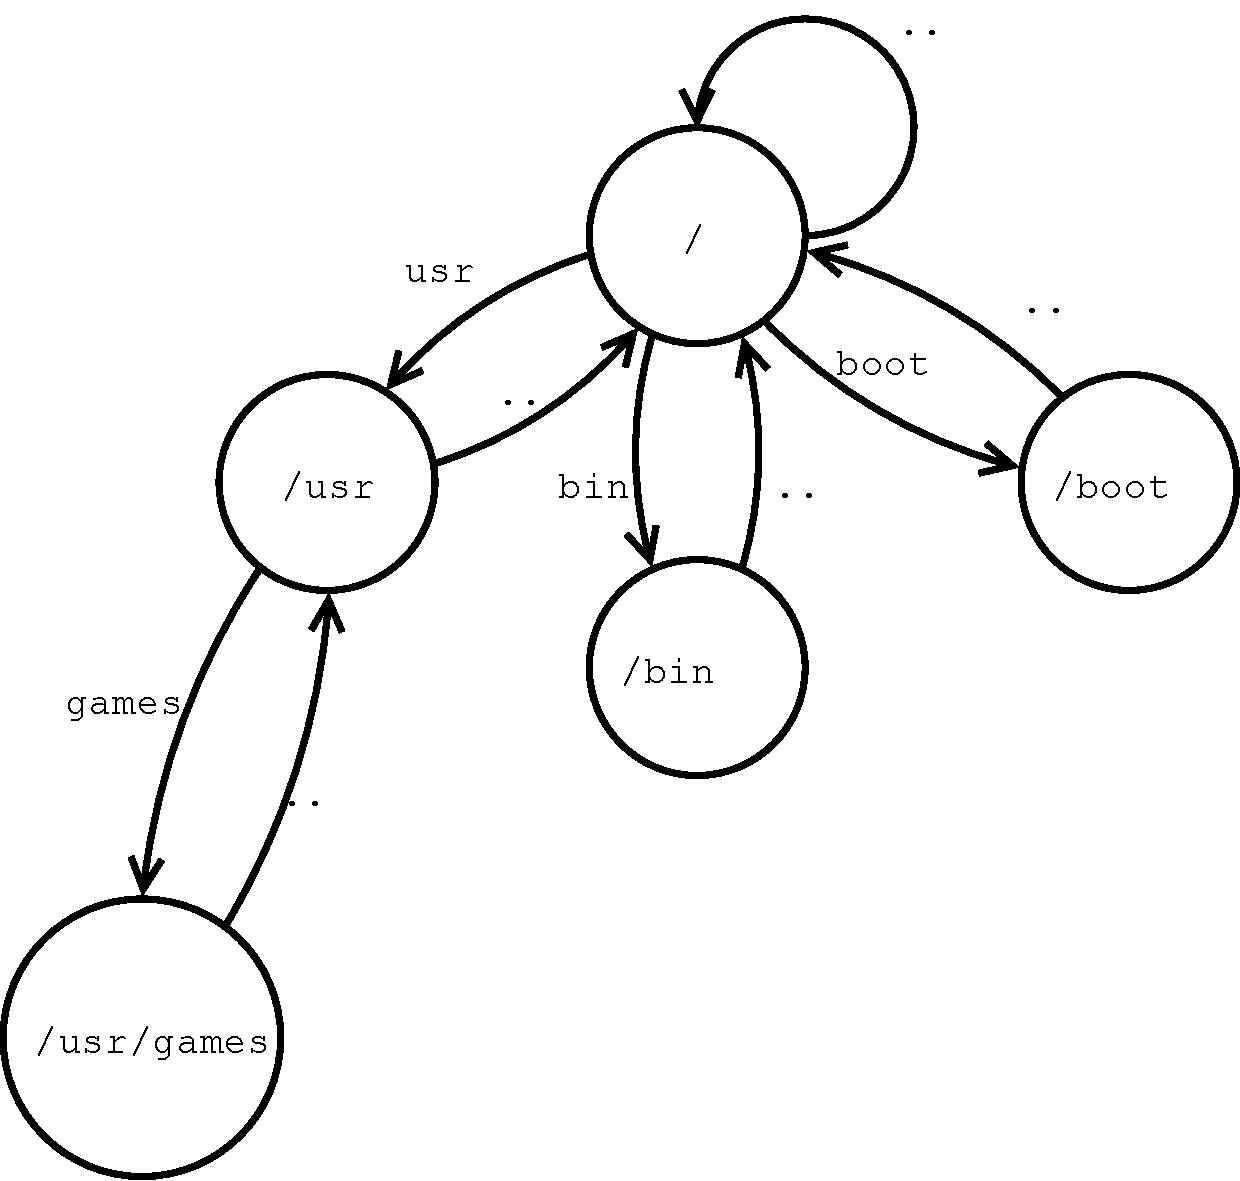
\includegraphics[width=\linewidth]{filesystems}
    \caption{Example of a filesystem}
    \label{img:extensions}
\end{figure}

In this figure, each directory has those inside it linked to it, and all of them
show where the directory \verb!..! which is inside them goes. As you can see, to
reach a path like \verb!/usr/games! we only have to ``hop'' from a directory to
the next. If we wanted to come back, we can use the fictional directories that
point to the parent of the directory we're in (\verb!..!).

The case of the root
directory is special, because its parent directory is the same directory. In
Windows the system is similar, but there is not only one root, there are
several. Those being the different storage drives we have. Also, we do not need
to be all the time hoping in one level jumps, we can use complete paths to
navigate from a place to the other. If you haven't figured it out yet by the
context, a path is simply the succession of directories that go from one to
another. There are two types of paths:
\begin{enumerate}
    \item Absolute paths: Those are the ones that start by slash, and they
    indicate a path from the root directory to a concrete directory or file.
    For example: \verb!/home/john/music/Beethoven_symphony.mp4! would be and
    absolute path.
    \item Relative paths: they are those that do not start from the root
    directory, but from the work directory. For example:
    \verb!music/Beethoven_symphony.mp4! is relative path that will point to
    an existing file only if inside the current work directory there is a
    directory called \verb!music! and, inside it, a file named
    \verb!Beethoven_symphony.mp4!.
\end{enumerate}

The text that shows up everytime you hit enter is called a prompt and, in
general, it shows you your username, the machine where you are and after that,
your working directory, if it fits in the screen. I am going to substitute
the prompt just for a dollar sign in the examples I show you, so it fits better
in the page. When you first started your terminal it showed a tilde (\verb!~!)
because that's an alias of your home directory, which is a route in Linux
systems where the user stores his personal files. Generally speaking, that
route is in \verb!/home/<username>! for example \verb!/home/john!.

Now we are going to learn to see what is inside a directory, the command that
allows us to do so is \verb!ls!, if you type it and hit enter you'd see...
nothing. That's because we have not created any file in our home directory,
the command to create files is called \verb"touch". Write \verb!touch test.txt!
and hit enter, if you now perform \verb!ls!, you would see it will show up.

\noindent
\begin{minipage}[H]{\linewidth}
\mbox{}
\begin{lstlisting}[style=terminalStyle]
\$ touch test.txt
\$ ls
test.txt
\$
\end{lstlisting}
\end{minipage}

\verb!ls! has a lot of options, options of Linux commands are set with a dash
infront of them, so, if you're told ``\verb!ls! with the options a and l'' you
must write \verb!ls -l -a! or, joining all them in the same dash: \verb!ls -la!
Something like this should appear on the screen.

\noindent
\begin{minipage}[H]{\linewidth}
\mbox{}
\begin{lstlisting}[style=terminalStyle]
\$ ls -la
total 8
drwxr-xr-x 1 john john  512 Jul  8 19:05 .
drwxr-xr-x 1 root root  512 Jul  7 22:37 ..
-rw-r--r-- 1 john john  220 Jul  7 22:37 .bash_logout
-rw-r--r-- 1 john john 3771 Jul  7 22:37 .bashrc
drwxr-xr-x 1 john john  512 Jul  7 22:37 .landscape
-rw-rw-rw- 1 john john    0 Jul  8 18:25 .motd_shown
-rw-r--r-- 1 john john  807 Jul  7 22:37 .profile
-rw-rw-rw- 1 john john    0 Jul  8 19:05 test.txt
\end{lstlisting}
\end{minipage}

As you can see, there are many files you have not created. This is because the
\verb!a! option makes \verb!ls! to show us \textbf{all the files}, including the
hidden ones, which are hidden because their name starts with a dot. The option
\verb!l! makes the command to show the files in a list, with more information
about them. If this is a bit intimidating to you, it is normal, and I have good
news. WSL sees the directories you have in you Windows system, so you can create
a folder in your desktop and work with the Windows explorer, to create or delete
files.

\subsection{Installing the compiler}
Now we already have a Linux installed in the computer, let's install the
compiler. To do that, we are going to execute the commands the are shown next.
If while executing any of them you are asked if you want to go ahead, answer
yes.

\noindent
\begin{minipage}[H]{\linewidth}
\mbox{}
\begin{lstlisting}[style=terminalStyle]
$ sudo apt update
#Lots of text will be shown here, don't mind it.
$ sudo apt install build-essential
........
After this operation, 189 MB of additional disk space will be used.
Do you want to continue? [Y/n] y
........
\end{lstlisting}
\end{minipage}

Now you should have the compiler installed, it is called GCC, it is an achronym
meaning GNU Compiler Collection. To see if that is the case, type the following
command. And check the output is similar to the one shown here.

\noindent
\begin{minipage}[H]{\linewidth}
\mbox{}
\begin{lstlisting}[style=terminalStyle]
\$ gcc -v
Using built-in specs.
COLLECT_GCC=gcc
COLLECT_LTO_WRAPPER=/usr/lib/gcc/x86_64-linux-gnu/9/lto-wrapper
OFFLOAD_TARGET_NAMES=nvptx-none:hsa
OFFLOAD_TARGET_DEFAULT=1
Target: x86_64-linux-gnu
Configured with: ../src/configure -v --with-pkgversion='Ubuntu 9.3.0-17ubuntu1~20.04' --with-bugurl=file:///usr/share/doc/gcc-9/README.Bugs --enable-languages=c,ada,c++,go,brig,d,fortran,objc,obj-c++,gm2 --prefix=/usr --with-gcc-major-version-only --program-suffix=-9 --program-prefix=x86_64-linux-gnu- --enable-shared --enable-linker-build-id --libexecdir=/usr/lib --without-included-gettext --enable-threads=posix --libdir=/usr/lib --enable-nls --enable-clocale=gnu --enable-libstdcxx-debug --enable-libstdcxx-time=yes --with-default-libstdcxx-abi=new --enable-gnu-unique-object --disable-vtable-verify --enable-plugin --enable-default-pie --with-system-zlib --with-target-system-zlib=auto --enable-objc-gc=auto --enable-multiarch --disable-werror --with-arch-32=i686 --with-abi=m64 --with-multilib-list=m32,m64,mx32 --enable-multilib --with-tune=generic --enable-offload-targets=nvptx-none=/build/gcc-9-HskZEa/gcc-9-9.3.0/debian/tmp-nvptx/usr,hsa --without-cuda-driver --enable-checking=release --build=x86_64-linux-gnu --host=x86_64-linux-gnu --target=x86_64-linux-gnu
Thread model: posix
gcc version 9.3.0 (Ubuntu 9.3.0-17ubuntu1~20.04)
\end{lstlisting}
\end{minipage}

If you get a similar text, congratulations, you have installed the C compiler.
Now we are going to, finally, start learning the concepts of the language.

\section{Your first program; say hello to the world!}

Let's navigate into that folder you have in the desktop. Units of your Windows
computer (the drives C, D, E...) are presented in the WSL as directories inside
the path \verb!/mnt!. So, \verb!C:! will be under \verb!/mnt/c!. I leave next an
example on how to navigate to a folder called \verb!hello_world! in your Windows
desktop. You can create it as you're used to now.

\noindent
\begin{minipage}[H]{\linewidth}
\mbox{}
\begin{lstlisting}[style=terminalStyle]
\$ cd /mnt/c/Users/John/Desktop/
\$ cd hello_word
\$ pwd
/mnt/c/Users/John/Desktop/hello_world
\$
\end{lstlisting}
\end{minipage}

Now you are already in the folder, open it in the file explorer, because we
have the last configuration left. In the Windows file explorer, in the top of
the window, click on the View tab and check the box next to ``show extensions
of known file types''. Next there is a picture of how it looks.

\begin{figure}[H]
    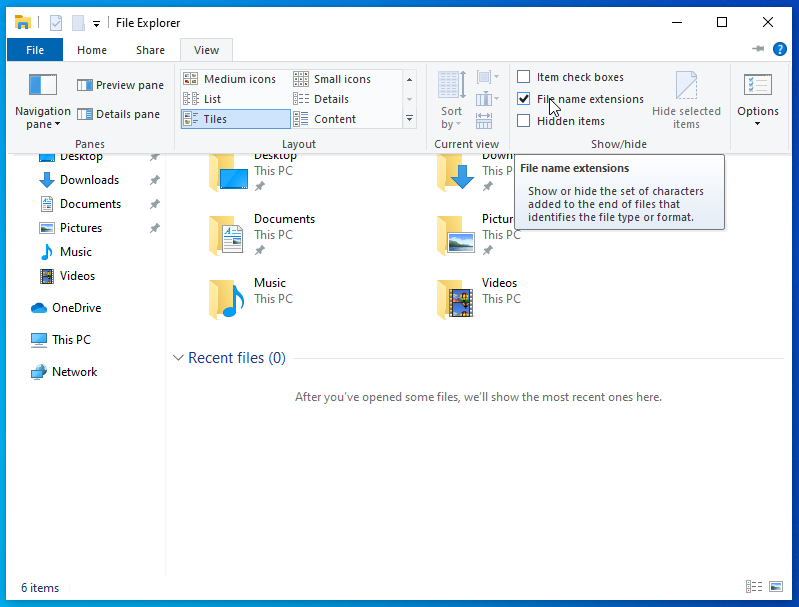
\includegraphics[width=\linewidth]{extensions_en}
    \caption{Configure how to see the extensions of known file types}
    \label{img:extensions}
\end{figure}

Now, in the way you like the most (the terminal or the mouse), create a file
in that folder called \verb!hello_world.c!. Open it with the Windows Notepad,
and I mean the Notepad, I do not mean WordPad, or Word. In that document we are
going to write the following.

\begin{figure}[H]
\begin{verbatim}
#include <stdio.h>

int main(void)
{
    printf("Hello, world!\n");
}
\end{verbatim}
\end{figure}

I want to clarify that the line that is displaced to the right is so because it
has spaces in the left side. You can write two, four or eight, I recommend four
as a general rule. Save the file, and go back to the terminal. You should have
the file in the directory. Make \verb!ls! to check it is in. Also, remember you
need to navigate to the folder if you closed the terminal or changed work
directory. Now we are going to compile our first program. To do that, we will
invoke GCC. I will list the commands and their expected output next.

\noindent
\begin{minipage}[H]{\linewidth}
\mbox{}
\begin{lstlisting}[style=terminalStyle]
\$ ls
hello_world.c
\$ gcc -o hello_world.elf hello_world.c
\end{lstlisting}
\end{minipage}

When doing this, a new file will appear in the directory, called
\verb!hello_world.elf!. Congratulations! that is your first program in C. What
does it do? It prints ``Hello, world!''. If you make double click on it, you
will see that Windows does not know how to open it. That is because it is a
Linux executable. Because of that, in the terminal, write
\verb!./hello_world.elf!. If you remember what I told you before, a path that
does not start with the root directory is a relative path, and the directory
dot \verb!.! is a relative path. When the terminal gets a command from the user,
it looks for a program with that name in a series of directories that are
configured in your operating system. If you want to execute any other program
(or other things you can execute, but I won't get tangled on them) you must
indicate a path, relative or absolute. To make the terminal understand we are
introducing a path and not a command, we start it by dot, that is, this very
directory. When you hit enter, you should see something like this:

\noindent
\begin{minipage}[H]{\linewidth}
\mbox{}
\begin{lstlisting}[style=terminalStyle]
\$ ./hello_world.elf
Hello, world!
\end{lstlisting}
\end{minipage}

You have compiled your first program, maybe you are a bit disappointed,
since you do not understand what it does, or how it does it. Hence it is the
moment we adquire a compromise with each other. That is, if you do not
understand something that appears in the programs we are going to see together,
you will trust I will clarify eventually when the moment arrives, from my side,
my compromise is that I will do it the earliest I can, so you have to put the
least amount of effort in ignoring things you don't know.

For now, I will explain what the command we have issued before is, gcc is, as
I said before, the C compiler, the option \verb!o! (remember that I explain
what options were when I explained you how to use \verb!ls!) indicates that the
next thing we are going to write is the name of the program we want to create
and, finally, the name of our source code file. If you put \verb!main.elf! the
resulting file would be called that, or anything you wanted, I'll be compiling
my programs as to files called \verb!main.exe! mainly.

\subsection{Text editor}
You edited your first program with the notepad, but editing code in that way
is a bit unbearable. Partially this is so because it is usual to use specialized
editors that colorize the words that are important in the concrete programming
language you are using and help you with things like knowing where the bracket
that closes the one your looking at now. I am going to leave here a list of
some common editors used with C code. I will not assume you are using any
concrete one, so choose the one you like. I use the first one, but maybe for
your first steps you may stick to Notepad++, which is simpler, and jump
to another one when you feel more comfortable writing more complex programs.
\begin{enumerate}
    \item Visual Studio Code.
    \item Atom.
    \item Sublime text
    \item Notepad++
\end{enumerate}

\section{First steps}

Now you already know what a source code file is I am going to show you how we
are going to include code fragments in the manual. Let's revisit the program
\verb!hello_world.c!.

\noindent
\begin{minipage}[H]{\linewidth}
\mbox{}
\begin{lstlisting}[style=C, caption={Hello World in C},
label={lst:helloWorld}]
#include <stdio.h>
int main(void)
{
    printf("Hello, world!\n");
}
\end{lstlisting}
\end{minipage}

As you can see, the lines are numbered, and there are words in blue, and others
in red. The blue word are the ones called key words, for now, remember that
all your programs must contain the lines 1, 2, 3 and 5 and that, between the
lines 3 and and 5 you will write the instructions that will make up your source
code files.

\subsection{Variables}

We are getting into business, at last! One of the first things that are needed
in a program are \textbf{variables}, a variable is an abstraction to designate a
space in the memory of the computer in which we store things. When we create a
variable we say to the computer: ``save this space in your memory to store
data''. C is a language of the kind we call typed, that is, each variable has a
type and cannot change that type after it is created. In C there is a set of
basic types that I will show you in a handy table.

\begin{table}[H]
    \centering
    \begin{tabularx}{\linewidth}{|c|c|c|Y|}
        \hline
        \textbf{Name} &\textbf{Size} (in bytes)&\textbf{Range}&\textbf{Ussage} \\\hline
        \texttt{char} & 1 & $[-128, 127]\vphantom{\matrix{1\cr1\cr1\cr}}$ & One text character or a byte\\\hline
        \texttt{short}& 2 & $[-32\,768, 32\,767]\vphantom{\matrix{1\cr1\cr1\cr}}$& Number in that range (generally network ports)\\\hline
        \texttt{int}&   4  & $[-2\,147\,483\,648, 2\,147\,483\,647]\vphantom{\matrix{1\cr1\cr1\cr}}$&General type for integer numbers\\\hline
        \texttt{float}& 4 & $[\pm3.4\cdot{}10^{-38}, \pm3.4\cdot{}10^{38}]\vphantom{\matrix{1\cr1\cr1\cr}}$ & Simple precision decimal numbers\\\hline
        \texttt{double}&8 &$[\pm1.79\cdot{}10^{-308}, \pm1.79\cdot{}10^{308}] \vphantom{\matrix{1\cr1\cr1\cr}}$ & Double precision decimal numbers\\\hline
    \end{tabularx}
    \caption{Basic types of C}
    \label{tab:basicTypes}
\end{table}

A table like that one may be intimidating at first, but it is simple. When we
declare (create) a variable, we must say what type it has. I like to say that
variables are like boxes and that, according to their type, inside that box
some things fit and some others do not. To declare a variable, you write its
type and a name, and do not forget to end the line with a semicolon (;)! Apart
from declaring them, we must learn to give them a value. That is called ``assign
a value'', and it is done with the equal sign (\verb!=!). To give it a value you
write the name of the variable, the equal sign and the value, let's see some
examples and I'll get into some caveats.

Regarding the name: the name of a variable is made out of letters, numbers and
underscores. The name of a variable must not be written all in uppercase, but
it can contain some. It cannot start by a number, and \textbf{you should not start
it with an underscore}. In general, you can use two notations to write variable
names in C (and in any programming language):
\begin{enumerate}
    \item \textbf{Camel case}: if a name contains several words, they must be
    written together, with the first letter of each word in uppercase,
    excluding the first. For example: \verb!betterValue! or \verb!targetNumber!.
    It is called like this
    because the uppercase letters remind of the humps of a camel.
    \item \textbf{Snake Case}: The words are separated by underscores, all in
    lowercase, for example:  \texttt{better\_value} or \texttt{target\_number}. It is
    called like that because the shape of the names written in this fashion
    remind of a snake that has eaten animals and has bulges in its body.
\end{enumerate}

\noindent
\begin{minipage}[H]{\linewidth}
\mbox{}
\begin{lstlisting}[style=C, caption={Declaration and assignment of variables},
label={lst:variableAsignation}]
#include <stdio.h>
int main(void)
{
    char letter = 'a';
    char byte = 120;
    short shorty = 5520;
    int money_i_want;
    float money_i_have = 3.22F;
    double money_you_have = 52.55;

    money_i_want = 450000;
    shorty = 11111;
}
\end{lstlisting}
\end{minipage}

Computers do not understand about letters, only numbers, therefore, when you
tell the computer that \verb!letter! is equal to \verb!'a'!, you tell it it's
equal to the number that letter has assigned. Mind that to assign the value
of a \verb!char! you must use simple straight quotes. The correspondency between
letters and numbers is written in the ASCII table, if you want to read it, I
leave this \href{https://www.ascii-code.com/}{link} to a site where u can
check it up. If you look there, you will see that the letter a has the value
97. After that, we assign to other char a numeric value, in line 7 you can see
we declare a variable without assigning a value to it. That is totally okay, but
beware!, \textbf{a variable to which you have not assigned a value has a random
one}. This is why many teachers would advice you that everytime you declare a
variable you should give it a value immediately. This process (giving value to
a variable for the first time) is called ``initialize'' a variable.

In lines 11 and 12 we give value to variables that we have declared before,
and I want to take some time talking about line 12. At first, it could seem
that when writing \verb!shorty = 5520;! we are enunciating a mathematical
equality, that that is always going to be the same, but in C we do not work with
``laws'', but with instructions, so you shall not read that line as ``the value
of shorty is 5520'' but ``I have assigned the value 5520 to shorty''. That is:
you have put into the ``box'' a 5520, but nothing avoids you to pull that
value out and put another one in as we do in line 12.

The values a programmer writes in the source code are called ``literals''. I
think that the name is pretty much self explanatory. Each literal has a type,
in the same way variables have. Later we will see why that's important. For now,
remember that literal is the name of values the programmer writes
explicitly in the code. That would be, numbers (like 5520) or letters,
(like \verb!'a'!). Apart from literals, we can assign to a variable the
value of an \textbf{expression}, a expression is any text written in the C
language that has a value. For now, we are going to limit ourselves to assign
one variable to other variables.

\noindent
\begin{minipage}[H]{\linewidth}
\mbox{}
\begin{lstlisting}[style=C, caption={Assigning variables to other variables},
label={lst:variableAsignationBetween}]
#include <stdio.h>
int main(void)
{
    int a = 3;
    int b = 2;

    a = b;
}
\end{lstlisting}
\end{minipage}

In line 7 we can see how I assign to the variable \verb"a" the value of the
variable \verb!b!, therefore, it will have a value of 2, now. Since seeing this
is difficult, I am going to include in the next example a series of lines with
the word \verb!printf! in them, you may remember it from our first program.
Later on, I will teach you to use it, but, at the moment, simply copy this
program in your source code file and compile it as we did before. (Copying
things from a PDF tends to be troublesome, therefore type it yourself, also, it
will serve as typing practice.)

\noindent
\begin{minipage}[H]{\linewidth}
\mbox{}
\begin{lstlisting}[style=C, caption={Final example of variable using},
label={lst:variableFinalExample}]
#include <stdio.h>
int main(void)
{
    int a = 3;
    int b = 10;
    printf("a is equal to: %d\n", a);
    a = b;
    printf("b is equal to: %d and a is the same, that is: %d\n", b, a);
    b = 22;
    printf("b is equal to: %d, a still is %d\n", b, a);
}
\end{lstlisting}
\end{minipage}

If you type this program, compile it and execute it, you should see something
like this:

\noindent
\begin{minipage}[H]{\linewidth}
\mbox{}
\begin{lstlisting}[style=terminalStyle]
\$ ./main.exe
a is equal to: 3
b is equal to: 10 and a is the same, that is: 10
b is equal to: 22, a still is 10
\end{lstlisting}
\end{minipage}

As you can see, when \verb!a = b! is written, \textbf{the values of a and b are
not linked together}. Nevertheless, when assigning any value to a variable, you
must be careful. Going back to the methaphor of the boxes, in a box you can fit
things of a certain set of shapes and sizes. If a data is, for instance, a
decimal number (wether it is a float or a double) if it is assigned to an
integer variable it will lose its decimal part. But there is more, if you apply
this logic, what would happen if you assign a number such as 1203 to a
\verb!char!? If you go to the table \ref{tab:basicTypes}:
\nameref{tab:basicTypes}, you will see that 1203 is outside the range of
\verb!char!. What happens is... you do not know what happens. The elegant way of
saying this is: ``undefined behaviour''. The next program is an example of that.


\noindent
\begin{minipage}[H]{\linewidth}
\mbox{}
\begin{lstlisting}[style=C, caption={Erroneous assignments},
label={lst:invalidAssignations}]
#include <stdio.h>
int main(void)
{
    char c = 1500;
    short s = 5555555;
    float f = 3.8e105;

    printf("c: %d\n", c);
    printf("s: %hd\n", s);
    printf("f: %f\n", f);
}
\end{lstlisting}
\end{minipage}

If you compile it, the compiler will throw a series of messages called warnings.
Those warnings warn you that, while something is correct, it seems it contains
some error. For example, if you wrote ``I did not know your Belgian'' the
sentence would be technically correct, it would mean you didn't know a Belgian
thing related in some way to the person you're talking to, regardless, more
probably, you wanted to say  ``I did not know you're Belgian ''. If we compile
and execute, something like the following should appear in the terminal.

\noindent
\begin{minipage}[H]{\linewidth}
\mbox{}
\begin{lstlisting}[style=terminalStyle]
\$ gcc -o main.exe main.c
main.c: In function 'main':
main.c:86:14: warning: overflow in conversion from 'int' to 'char' changes value from '1500' to '-36' [-Woverflow]
   86 |     char c = 1500;
      |              ^~~~
main.c:87:15: warning: overflow in conversion from 'int' to 'short int' changes value from '5555555' to '-15005' [-Woverflow]
   87 |     short s = 5555555;
      |               ^~~~~~~
\$ ./main.exe
c: -36
s: -15005
f: inf
\end{lstlisting}
\end{minipage}

As you can see, neither the \texttt{char} is equal to 1,500 nor the
\texttt{short} is 5,555,555, because they cannot be. The compiler does not say
anything about the \texttt{float} or the \texttt{double}, the reason is that
both data types have a special value called infinity, which symbolizes infinity.
This is because, as we will see later on, they do not represent numbers in a
totally correct way, and that's why they can be positive and negative infinity.

Let's take some time for the problem of decimal numbers. If you know how binary
code works, you would know that a binary number of $n$ digits you can represent
$2^n$ numbers. In the case of decimal numbers, we use one complex system called
IEEE 754. I am not going to go into detail here, but the main problem of this
way of representing numbers is that it is not only not exact (for example,
the number 0.1 cannot be represented exactly), but its precission is not
constant. What does this mean? That if near the zero the float may distinguish
between 1.10 and 1.11, it is possible they cannot distinguish 10000000.10 from
10000000.11. Be careful about that when you use decimal numbers.

As you have seen here, there are allowed assignments and forbidden ones. The
allowed ones (those the compiler does not see as something bad), are called
implicit conversions, the name comes from the fact you do not need to do
anything to make them happen, for example, assigning a char value to an integer
variable. Later on I will teach you to perform conversions between data types
explicitly.

\subsection{Printing things}
Programmers call ``print'' to write things into files and, specially, in the
screen, like your first program that wrote ``Hello, world!''. I do not want to
get ahead of myself, because there are several concepts behind what we use to
print things on the screen, nevertheless, I need you to be able to show things
on the screen to be able to test your own programs.

To print things on the screen you must use the word \texttt{printf}. With a
syntax (syntax just means the way things are suppossed to be written) a little
bit difficult. You must write \texttt{printf}, an opening parenthesis and a thing
called ``format'' which is the text that is going to be printed, surrounded by
double straight quotes (\texttt{"}). To include variables in that printing, you
must put ``specifiers'', which are special texts that signal \textbf{the type}
of the variables you want to print. After the format, we will write the
variables we are going to print, separated by commas, in the order we wrote
their specifiers. Also, there are some special characters you must write in a
special manner: the new lines and the tabulators. This is a bit confusing, so
I will show you two tables where you can see the specifiers and the special
characters.

\begin{table}[H]
\centering
\begin{tabularx}{\linewidth}{|c|Y|}
\hline
\textbf{Specifier} & \textbf{Type it prints}                                                    \\ \hline
\texttt{\%d}& Integers (\texttt{int})                                                           \\ \hline
\texttt{\%f}& \texttt{float}                                                                    \\ \hline
\texttt{\%lf}& \texttt{double}                                                                  \\ \hline
\texttt{\%hd}& \texttt{short}                                                                   \\ \hline
\texttt{\%c}& \texttt{char} as characters (no numbers)                                          \\ \hline
\texttt{\%s}& Text, written as \texttt{\textquotedbl A text\textquotedbl}, quotes included.      \\ \hline
\texttt{\%p}& Pointers, they are an advanced feature of the language, I will explain them later \\ \hline
\end{tabularx}
\caption{Format specifiers}
\label{tab:formatSpecifierC}
\end{table}

On the other hand, the special characters are these, and are written with a
backwards slash (\textbackslash{}) infront of them. In the table I already
included the backward slash. Also, since the specifiers are written starting with
percentage symbol (\verb!%!), if you want to print it, you need to put it twice.

\begin{table}[H]
\centering
\begin{tabularx}{\linewidth}{|c|Y|}
\hline
\textbf{Sequence} & \textbf{Printed character}                       \\\hline
\texttt{\textbackslash{}\textbackslash{}} & Backwards slash          \\\hline
\texttt{\textbackslash{}n}& New line                                 \\\hline
\texttt{\textbackslash{}t}& Tabulator (prints spaces until the next character is aligned with four character column in the terminal) \\\hline
\texttt{\%\%}& Will print just one percentage symbol.                \\\hline
\end{tabularx}
\caption{Sequences to print special characters}
\label{tab:specialCharsC}
\end{table}

This is a bit dry, let's see an example.

\noindent
\begin{minipage}[H]{\linewidth}
\mbox{}
\begin{lstlisting}[style=C, caption={Ejemplo de impresión.},
label={lst:decimalvsintergerDivision}]
#include <stdio.h>
int main(void)
{
    int integer = 654654;
    short shorty = 25254;
    char charty = 'a';
    double decimal = 2.3;
    printf("The integer is:\t%d\nThe short is:\t%hd\nThe char is the letter:\t%c\nThe decimal number is:\t%f\n", integer, shorty, charty, decimal);
}
\end{lstlisting}
\end{minipage}

The line is very long and in this page is it written as many, but you should
write it as a single line. If you look closely, there is only one line number,
that indicates that it's the same line but it is broken so it fits in the page.
The program, once compiled and executed, should print something like this.

\noindent
\begin{minipage}[H]{\linewidth}
\mbox{}
\begin{lstlisting}[style=terminalStyle]
\$ ./main.exe
The integer is: 654654
The short is:   25254
The char is the letter: a
The decimal number is:  2.300000
\end{lstlisting}
\end{minipage}

As a bottom line: \texttt{printf} does not add anything you do not put in it,
like new lines, so if you want to print the next thing in a new line, remember
to write \verb!\n! at the end of the format. Also, it is good that your program
prints a new line character as the last thing, if not, it could leave things
unprinted. That's because the terminal forces itself to print everything you
have ordered it to print when it finds a new line.

\subsection{Operators}
Playing a shell game with the values of the variables you declare in a program
is boring, I know, therefore we are going to learn to perform operations with
them. In C (and in any other programming language) there are the so called
\textbf{operators}. They are symbols that allow us to perform calculations.
Operators are a mathematical concept, and are applied to a set of arguments, or
better put, operands. In math, the symbols $+$, $-$, $\times$ and $\div$ are
mathematical operators for addition, substraction, multiplication and division,
respectively. In the same way we have done with the basic types, I will present
the operators in a table and later on we will see examples on how to use them.

\begin{table}[H]
\centering
\begin{tabularx}{\linewidth}{|c|Y|}
\hline
\bf Operator & \bf Description \\ \hline
\tt + & Addition. Adds integers and decimals together and between them. \\\hline
\tt - & Substraction. Substracts from the left operand the value of the right operand. \\\hline
\tt / & Division. Returns the result of the division of the left operand by the right one. Note that, \textbf{if both operands are integers}, the operator performs integer operation, that is, \textbf{without decimals}. \\\hline
\tt * & Multiply. Asterisk has many functions in C, but this is the first of them you will discover. The type of the multiplication of two integer is always a \textbf{double}.\\\hline
\tt ++ & Increment. Makes a number (either integer or decimal) go up one unit, it can be prefix (before the operand) or postfix (after the operand).\\\hline
\tt -{}- & Decrement. Works as the increment, but it makes the number to go down one unit. \\\hline
\tt \% & Module. Is an operator that return the residue of the division of the left operand by the right operand. \\\hline
\end{tabularx}
\caption{Basic math operators in C}
\label{tab:mathOperators}
\end{table}

In the last section I told you that we could assign a value to a variable.
I also told you that an expression is a fragment of C code with a value, and
that the name of a variable alone is an expression. Now we have operators, we
can write more complex expressions, for example \verb!a+b! would be an
expression whose value would be the addition of a and b.
We can make calculations now!

You must be careful, though, because, as I said before, all expression in C has
a \textbf{type} and, as we saw in the last section, assigning a value of
incorrect type to a variable is error prone. For example, the operator division
behaves differently if the operands (the numbers we're dividing) are integer or
decimal. Let's see and example.

\noindent
\begin{minipage}[H]{\linewidth}
\mbox{}
\begin{lstlisting}[style=C, caption={Integer division vs decimal division},
label={lst:decimalvsintergerDivision}]
#include <stdio.h>
int main(void)
{
    double d1 = 1/3;
    printf("d1: %f\n", d1);

    double d2 = 1.0/3;
    printf("d2: %f\n", d2);
}
\end{lstlisting}
\end{minipage}

If you compile and execute the problem you will see this result:

\noindent
\begin{minipage}[H]{\linewidth}
\mbox{}
\begin{lstlisting}[style=terminalStyle]
\$ ./main.exe
d1: 0.000000
d2: 0.333333
\end{lstlisting}
\end{minipage}

What would look like the same operation gave totally different results, and this
is because the \textbf{type} of the operands was different. In C, a literal
integer number value is an \texttt{int}, and the division operator when it
is operating on two integers, has an integer type. Nevertheless, when
\textbf{any of the two} operands is decimal, the operator performs the decimal
division, and its type is \texttt{double}.

Operators \verb!++! and \verb!--! are special, because they are unary operators.
An unary operator is an operator that is applied only to one operand. For
example, in math you have the operator square root, whose symbol is
$\sqrt{\phantom{2}}$ which, applied to just one number, gives us the number
(or numbers) that squared give us the operand. The operators increment and
decrement are unary and, also, can be written infront or behind the operand.
These are special operantors that do not only give us a value, but also
\textbf{affect the value of the operand they act on}. Simply: if \verb!a! is
equal to three and we make \verb!a++!, \verb!a! will be four, but if we assign
the value of the operation to other variable, that other variable will have
a different value depending on if we write it in the postfix or prefix way,
let's see it in the code.

\noindent
\begin{minipage}[H]{\linewidth}
\mbox{}
\begin{lstlisting}[style=C, caption={Increment and decrement operators},
label={lst:prefixAndPostfixOperators}]
#include <stdio.h>
int main(void)
{
    int a = 3;
    int b = ++a;
    printf("a: %d; b: %d\n", a, b);
    a = 3;
    int c = a++;
    printf("a: %d; c: %d\n", a, c);
}
\end{lstlisting}
\end{minipage}

If you execute it, you'll see the following.

\noindent
\begin{minipage}[H]{\linewidth}
\mbox{}
\begin{lstlisting}[style=terminalStyle]
\$ ./main.exe
a: 4; b: 4
a: 4; c: 3
\end{lstlisting}
\end{minipage}

I want you to understand precisely what is happening here: everytime we apply
the operand increment to a variable, that variable will increment
its value in one unit. Nevertheless; depending on if we write it as prefix
(infront the variable) or postfix (after it) the expression itself will have one
value or another. If we do it prefix, the value
of the expression of the operation
would be the value of \verb!a! \textbf{after} it increments its value, if we
do it as a postfix operator, the value will be \textbf{before the increment}.

Following the line of increment and decrement operators, there are also
operators that put together the assignment with other mathematical operations,
that is, substituting for example \lstinline[style=C]!a = a * 3;! by
\lstinline[style=C]!a *= 3;!. The same style of operators exists for
substraction, addition, division and module.

Finally, we simply must tell that the \textbf{priority} of the operations
is the same than in mathematics: the first expressions to be evaluated are those
inside parenthesis, after them division and multiplication, both have
the same priority, so in case you have several mixed, you will execute them
from left to right. After that, addition and substraction that are, again,
executed from left to right.

\subsubsection{Casting: explicit conversions}
It is usual that one needs to convert one type into another, for example, in the
case we saw before with the division, if you wanted a decimal division, you
would need to make one of them decimal to get the result you want. It is also
common than a variable that is an \texttt{int} gets assigned to a \texttt{char}
because you know its result is inside the range of values a \texttt{char} can
hold. Casting is a word that means the process of putting molten metals inside
a shaped container what will make the metal to retain that shape when it
solidifies, is it a methaphor of what we are doing changing the type of a value.
Nevertheless, it has its limits, laws of logic still apply, and you
cannot make a \texttt{char} to hold more than 127, for example, regardless of
casting.

\noindent
\begin{minipage}[H]{\linewidth}
\mbox{}
\begin{lstlisting}[style=C, caption={Casting example},
label={lst:castingExample}]
#include <stdio.h>
int main(void)
{
    int a = 3;
    int b = 2;
    double result = (double)a / b;
}
\end{lstlisting}
\end{minipage}

In line 6 we need one of the operands to be decimal (either \texttt{float} or
\texttt{double}). We perform cast to that type on the first operand. The syntax
is easy, but I am going to explain it in detail. You must write the name
of the type you want to convert the value to between parenthesis and next to it
the expression you want to cast. I'll leave you a couple examples:
\begin{enumerate}
\item \lstinline[style=C]!(int) (decimal_number / other_decimal)!: here we are
casting to an integer type the result of a division, as you can see, we need
to enclose the whole division in parenthesis so the casting is not applied only
to the first element.
\item \lstinline[style=C]!(char) (number % 128)!: Here you can see one of the
instances in which casting some integer type to a smaller one is ok. If
\texttt{number} is an integer, by casting it to \verb!char! there could be
problems but since we have performed module on 128, the result of the expression
is going to be between 0 and 127, therefore we know it is going to be in range
of the \texttt{char}.
\end{enumerate}
Following there is a table that will tell you which conversions are allowed and which
are not possible.

\begin{table}[H]
\begin{tabularx}{\linewidth}{|c|c|Y|Y|Y|Y|Y|}
\cline{3-7}
\multicolumn{2}{c|}{}&\multicolumn{5}{c|}{\textbf{Destiny type}}\\\cline{3-7}
\multicolumn{2}{c|}{}& \texttt{char}&\texttt{short}&\texttt{int}&\texttt{float}&\texttt{double} \\\cline{1-7}
\multirow{5}{*}[-5em]{\begin{sideways}\textbf{Source type}\end{sideways}}&\texttt{char} &OK&OK &OK &OK &OK \\\cline{2-7}
&\texttt{short} &Casting (overflow)&OK&OK&OK&OK \\\cline{2-7}
&\texttt{int} &Casting (overflow) &Casting (overflow)& OK&OK (precission) & OK (precission)\\\cline{2-7}
&\texttt{float} &Casting (rounding, overflow)& Casting (rounding, overflow)& Casting (rounding, overflow)& OK& OK \\\cline{2-7}
&\texttt{double} &Casting (rounding, overflow)& Casting (rounding, overflow)& Casting (rounding, overflow)& Casting (rounding, overflow)&OK \\\cline{1-7}
\end{tabularx}
\caption{Type conversions in C}
\label{tab:conversions}
\end{table}

Where I write ``ok'' I mean that there is an implicit conversion, but you must
be careful, the range of the integer is big and you may find that the precission
of a \texttt{float} is not good enough in the bigger values to have
problems distinguishing one unit from the next. I am going to be sincere with
you, this does not happen, the \texttt{float} is precise enough in the limits
of the integer to tell whole units apart, but I write it in the table to remind
you that you may look at the precission of the decimals. Where I write casting
and I precise there can be an overflow I mean you're performing cast from
a bigger type to a smaller one, so that is not generally acceptable unless you
check yourself that the value of the casted expression fits into the new type.

\subsubsection{Final example of a program with operators}
At this point, we can make our first program that does ``something'', I am
going to give you an example that calculates the solution to a system of
linear equations, that is:

$$
\left\{\matrix{ax+by = c \cr
               dx+ey = f}
\right.
$$

With a system like that, we can apply substitution:
$$
(1)\; ax+by=c \to x= \frac{c-by}{a}
$$
$$
(2)\; dx+ey=f \to x=\frac{f-ey}{d}
$$
$$
(1) \;\mathrm{and} \; (2) \to \frac{c-by}{a} = \frac{f-ey}{d} \to
y=\frac{af-dc}{ae-db} \to x=\frac{f-e\cdot\frac{af-dc}{ae-db}}{d}
$$

\noindent
\begin{minipage}[H]{\linewidth}
\mbox{}
\begin{lstlisting}[style=C, caption={Linear equation system solving},
label={lst:linealEquation}]
#include <stdio.h>
int main(void)
{
    int a = 1;
    int b = 3;
    int c = 8;
    int d = 2;
    int e = 7;
    int f = 12;

    double y = (a * f - d * c) / (a * e - d * b);
    double x = (f - e * y) / (d);

    printf("%dx+%dy=%d\n", a, b, c);
    printf("%dx+%dy=%d\n", d, e, f);
    printf("x = %f; y = %f\n", x, y);
}
\end{lstlisting}
\end{minipage}

If you copy this program, compile and execute it, you would see that I have
explained about variables and expressions. Nevertheless, the program has a
problem: it only solves one system of equations, to change the system, we need
to change the source code and recompile. This is not practical, and real
programs do not work in this way. For now most of our programs would be like
this one, because I want to explain more fundamental things first. Up until
now our programs have been very boring, they are limited to execute a series of
instructions one after the other. In real life, though, programs execute
one set of instructions or other depending on conditions, or they repeat
certain instructions several times, etc.

Other problem of this program is that we cannot change the behaviour of it
in certain conditions. If you change the value of the numbers in the
program in a way you make the system irresolvable the program will fail.
Test it, change the values of \texttt{a}, \texttt{b} and \texttt{c} to 1 and
\texttt{d}, \texttt{e} and \texttt{f} to 2. This system has infinite solutions
and will make the program to fail. If you compile and execute with the new
values, you should get something like the following:

\noindent
\begin{minipage}[H]{\linewidth}
\mbox{}
\begin{lstlisting}[style=terminalStyle]
\$ ./main.exe
1x+1y=1
2x+2y=2
x = -nan; y = -nan
\end{lstlisting}
\end{minipage}

What in tarnation is a nan? It is one of the special values that decimal numbers
in C can hold (remember IEEE 754). It means ``Not and Number''.
So, the result of that operation is not a number. How is that
possible? Because we have divided by zero. If you know a little about calculus
you'd know that a number divided by zero is an indetermination, that is, we do
not know what it is. That's how C deals with that. And we are lucky, if instead
of a decimal division it were an integer division, the program would simply
close abruptly. It would be interesting to check if the system has a solution,
and, if it had, then calculate it. This is done with control structures, which
will be explained in the next chapter.

\section{Changing the normal flow of the program}
As I introduced in the last section, it is convenient to be able to make the
program do one thing or the other according to a condition. Also, it is possible
(as a matter of fact it's essential) to repeat instructions according to
conditions. This is called altering the flow of the program, because instead
of execute one line after he next, the computer can jump from
a place to another, either forwards or backwards.

\subsection{Conditional sentences}
Conditional sentences are the ones that allow us to make the program flow
to \textbf{diverge}. You are going to understand it easily with the next
diagram.

\begin{figure}[H]
\centering
% generated by Plantuml 1.2022.7
\definecolor{plantucolor0000}{RGB}{34,34,34}
\definecolor{plantucolor0001}{RGB}{241,241,241}
\definecolor{plantucolor0002}{RGB}{24,24,24}
\definecolor{plantucolor0003}{RGB}{0,0,0}
\definecolor{plantucolor0004}{RGB}{17,17,17}
\begin{tikzpicture}[yscale=-1
,pstyle1/.style={color=plantucolor0002,fill=plantucolor0001,line width=0.5pt}
,pstyle4/.style={color=plantucolor0002,line width=1.0pt}
,pstyle5/.style={color=plantucolor0002,fill=plantucolor0002,line width=1.0pt}
]
\draw[color=plantucolor0000,fill=plantucolor0000,line width=1.0pt] (191.176pt,20pt) ellipse (10pt and 10pt);
\draw[pstyle1] (143.9784pt,50pt) -- (238.3736pt,50pt) -- (250.3736pt,62pt) -- (238.3736pt,74pt) -- (143.9784pt,74pt) -- (131.9784pt,62pt) -- (143.9784pt,50pt) -- cycle;
\node at (143.9784pt,55.0283pt)[below right,color=black]{(a * e - d * b) is 0};
\node at (113.0451pt,48.0566pt)[below right,color=black]{true};
\node at (250.3736pt,48.0566pt)[below right,color=black]{false};
\draw[pstyle1] (11pt,101.6055pt) arc (180:270:17.6055pt) -- (28.6055pt,84pt) -- (147.5078pt,84pt) arc (270:360:17.6055pt) -- (165.1133pt,101.6055pt) -- (165.1133pt,101.6055pt) arc (0:90:17.6055pt) -- (147.5078pt,119.2109pt) -- (28.6055pt,119.2109pt) arc (90:180:17.6055pt) -- (11pt,101.6055pt) -- cycle;
\node at (21pt,94pt)[below right,color=black]{Print: it has no solution};
\draw[pstyle1] (185.1133pt,101.6055pt) arc (180:270:17.6055pt) -- (202.7187pt,84pt) -- (385.8719pt,84pt) arc (270:360:17.6055pt) -- (403.4773pt,101.6055pt) -- (403.4773pt,101.6055pt) arc (0:90:17.6055pt) -- (385.8719pt,119.2109pt) -- (202.7187pt,119.2109pt) arc (90:180:17.6055pt) -- (185.1133pt,101.6055pt) -- cycle;
\node at (195.1133pt,94pt)[below right,color=black]{y = ( a * f - d * c ) / ( a * e - d * b )};
\draw[pstyle1] (225.1377pt,156.8164pt) arc (180:270:17.6055pt) -- (242.7432pt,139.2109pt) -- (345.8474pt,139.2109pt) arc (270:360:17.6055pt) -- (363.4529pt,156.8164pt) -- (363.4529pt,156.8164pt) arc (0:90:17.6055pt) -- (345.8474pt,174.4219pt) -- (242.7432pt,174.4219pt) arc (90:180:17.6055pt) -- (225.1377pt,156.8164pt) -- cycle;
\node at (235.1377pt,149.2109pt)[below right,color=black]{x = ( f - e * y ) / ( d )};
\draw[pstyle1] (191.176pt,180.4219pt) -- (203.176pt,192.4219pt) -- (191.176pt,204.4219pt) -- (179.176pt,192.4219pt) -- (191.176pt,180.4219pt) -- cycle;
\draw[color=plantucolor0000,line width=1.0pt] (191.176pt,235.4219pt) ellipse (11pt and 11pt);
\draw[color=plantucolor0004,fill=plantucolor0000,line width=1.0pt] (191.176pt,235.4219pt) ellipse (6pt and 6pt);
\draw[pstyle4] (294.2953pt,119.2109pt) -- (294.2953pt,139.2109pt);
\draw[pstyle5] (290.2953pt,129.2109pt) -- (294.2953pt,139.2109pt) -- (298.2953pt,129.2109pt) -- (294.2953pt,133.2109pt) -- cycle;
\draw[pstyle4] (131.9784pt,62pt) -- (88.0566pt,62pt);
\draw[pstyle4] (88.0566pt,62pt) -- (88.0566pt,84pt);
\draw[pstyle5] (84.0566pt,74pt) -- (88.0566pt,84pt) -- (92.0566pt,74pt) -- (88.0566pt,78pt) -- cycle;
\draw[pstyle4] (250.3736pt,62pt) -- (294.2953pt,62pt);
\draw[pstyle4] (294.2953pt,62pt) -- (294.2953pt,84pt);
\draw[pstyle5] (290.2953pt,74pt) -- (294.2953pt,84pt) -- (298.2953pt,74pt) -- (294.2953pt,78pt) -- cycle;
\draw[pstyle4] (88.0566pt,119.2109pt) -- (88.0566pt,192.4219pt);
\draw[pstyle4] (88.0566pt,192.4219pt) -- (179.176pt,192.4219pt);
\draw[pstyle5] (169.176pt,188.4219pt) -- (179.176pt,192.4219pt) -- (169.176pt,196.4219pt) -- (173.176pt,192.4219pt) -- cycle;
\draw[pstyle4] (294.2953pt,174.4219pt) -- (294.2953pt,192.4219pt);
\draw[pstyle4] (294.2953pt,192.4219pt) -- (203.176pt,192.4219pt);
\draw[pstyle5] (213.176pt,188.4219pt) -- (203.176pt,192.4219pt) -- (213.176pt,196.4219pt) -- (209.176pt,192.4219pt) -- cycle;
\draw[pstyle4] (191.176pt,30pt) -- (191.176pt,50pt);
\draw[pstyle5] (187.176pt,40pt) -- (191.176pt,50pt) -- (195.176pt,40pt) -- (191.176pt,44pt) -- cycle;
\draw[pstyle4] (191.176pt,204.4219pt) -- (191.176pt,224.4219pt);
\draw[pstyle5] (187.176pt,214.4219pt) -- (191.176pt,224.4219pt) -- (195.176pt,214.4219pt) -- (191.176pt,218.4219pt) -- cycle;
\end{tikzpicture}

\caption{Flow diagram: solving an equation system with a conditional}
\label{img:fluxIgEq}
\end{figure}

What you're seeing is called a flow diagram, despite the fancy name, it is very
easy to read. You start in the black dot in the top of the diagram,
and you follow the arrow, a diamond means a \textbf{decision}, according to what
is inside the decision (a condition), one branch or the other will be taken.
If you read the text of the condition inside the diamond, I have written there
what makes our system \textbf{irresolvable}. If you read the text next to the
arrows that come out from the diamond, you will see that if $ae-db=0$, we will
print that the system is not solvable and exit normally. If it is not zero,
we will continue doing what we were doing before.

\subsubsection{Logic operations}

This drawing is nice, but let's see how we do that in C. Now I have to present
to you another set of operators, called boolean operators or logic operators.
In the section \ref{section:queEsLaProgramacion} I mentioned logic as a science.
Concretely we are going to apply propositional logic, or first order logic.
In this logic we have \textbf{facts} that can be only \textbf{true} or
\textbf{false}, and they relate with each other with three operators. Let's see
an example, and then we will hop to the theory.

Imagine a fire extinguishing system that works in this manner: ``If the
temperature is greater than 50\centigrade, the fire sprinklers will start
working, if the temperature is lower, but there is smoke detected, the sprinklers
will start working anyway''. Since this is a science, let's write it in a formal
manner. Each sentence that is conceptually different is a \textbf{proposition},
and they're generally named by letters of the alphabet from p onwards. Let's
see which propositions we have:

\begin{enumerate}
    \item Temperature is greater than 50\centigrade, let's call it $p$.
    \item Smoke is detected, let's call it $q$.
    \item The sprinklers go off, let's call it $r$.
\end{enumerate}


\begin{table}[H]
\begin{tabularx}{\linewidth}{|c|c|Y|}
\hline
$T>50\;{}^{\circ}\mathrm{C}(\mathbf{p})$&Smoke$(\mathbf{q})$&Sprinklers go off$(\mathbf{r})$\\\hline
True  & True  & True  \\\hline
True  & False & True  \\\hline
False & True  & True  \\\hline
False & False & False \\\hline
\end{tabularx}
\caption{Example of logic operations}
\label{tab:logicOperationExample}%
\end{table}

In logic, there are thee basic operators:
\begin{enumerate}
\item Conjunction, commonly known as ``and''. It is written with the symbol $\land$.
\item Disjunction, common knows as ``or''. It is written with the symbol $\lor$.
\item Negation, commonly knows as ``not''. It is written with several symbols,
for example $\sim$ and $\lnot$, but it is written also putting a bar over the
negated expression, for example $\overline{p}$.
\end{enumerate}

\begin{table}[H]
    \centering
    \begin{subfigure}{0.33333\linewidth}
        \centering
        \begin{tabular}{|c|c|c|}
        \hline
        $\mathbf{p}$&$\mathbf{q}$&$\mathbf{p\land q}$\\\hline
        False & False  & False \\\hline
        False & True & False \\\hline
        True& False  & False \\\hline
        True& True & True\\\hline
        \end{tabular}
    \end{subfigure}%
    \begin{subfigure}{0.33333\linewidth}
        \centering
        \begin{tabular}{|c|c|c|}
        \hline
        $\mathbf{p}$&$\mathbf{q}$&$\mathbf{p \lor q}$\\\hline
        False & False  & False \\\hline
        False & True & True\\\hline
        True& False  & True\\\hline
        True& True & True\\\hline
        \end{tabular}
    \end{subfigure}%
    \begin{subfigure}{0.33333\linewidth}
        \centering
        \begin{tabular}{|c|c|}
        \hline
        $\mathbf{p}$&$\mathbf{\sim\!p}, \mathbf{\lnot p}, \mathbf{\overline{p}}$\\\hline
        True & False  \\\hline
        False & True \\\hline
        \multicolumn{2}{c}{\color{white}CIERTOFALSO\normalcolor}\\\arrayrulecolor{white}\hline
        \multicolumn{2}{c}{\color{white}CIERTOFALSO\normalcolor}\\\arrayrulecolor{white}\hline
        \end{tabular}
    \end{subfigure}
\caption{Tables of truth of the basic logic operations}
\label{tab:andTruthTable}
\end{table}

The conceptual meanings of the operations are intuitive, but I will explain it
here to tell some details. The conjunctios is true only when \textbf{both}
of the operand are true, and is like joining two propositions with ``and'' in
English. ``It is raining and it's cold'' is true only if at the same time it's
raining and it's cold. On the other hand, disjunction is when you join two
propositions with ``or''. ``I have twisted my anckle or I have broken it'', but
there is a caveat here, if you look at the truth table you will se that when
\textbf{both members}  are true, the disjunction is true also. It is something
that is not aligned with the spoken language, and you need to keep it in mind.
Finally, negation is when you put ``not'' before the expression or preposition,
``it is not raining'' is true only if ``it is raining'' is false.

And, after this logical detour that would make Aristotle proud, what?
We're almost there, in C the logic operators are written in this way:
\begin{enumerate}
    \item Conjunction is written: \verb!&&!.
    \item Disjunction is written: \verb!||!. (This symbols is called a pipe
    symbol, in the American keyboard you ir get pushing the key over the enter
    and shift.)
    \item Negation is written: \verb"!".
\end{enumerate}

If we go back to the example of the fire sprinklers, let's make a program that
``simulates'' the system, I will write it now.
Up until now I have talked about true and false values, in C that is represented
with an integer type (any of those available). Zero is the false value, and
\textbf{all the other values} are true. Generally the result of a logic
operation will be one if it's true, but you cannot assume that when using
an integer type to store logic values.

\noindent
\begin{minipage}[H]{\linewidth}
\mbox{}
\begin{lstlisting}[style=C,
caption={First program with logic operations},
label={lst:firstLogicProgram}]
#include <stdio.h>
int main(void)
{
    int temperature_greater_than_50 = 1;
    int smoke = 0;
    int sprinklers = temperature_greater_than_50 || smoke;
}
\end{lstlisting}
\end{minipage}

Yes, it looks like the boring programs we were doing up until now, do not worry,
the matter is: if you go back to \ref{tab:logicOperationExample}:
\nameref{tab:logicOperationExample} you're going to see that the program is just
a disjunction, if there is smoke, or the temperature is high, or both, the
sprinklers will go off. Nevertheless, this program is still a bit useless. We
cannot check is the temperature is greater or lower than 50 \centigrade, we have
had to make it up. This leads me to present another set of operators to you,
the comparison operators. This is easy, in C we can check is one variable
(or expression) is equals, greater or less than another. I will write the
table and let's improve the program we had before.
\begin{table}[H]
\centering
\begin{tabularx}{\linewidth}{|c|Y|}
\hline
\bf Operator & \bf Description \\ \hline
\tt < &   True is the left operand is less than the right one, false otherwise.\\\hline
\tt > &   True is the left operand is greater than the right one, false otherwise.\\\hline
\tt <= &  True is the left operand is less than or equal to the right one, false otherwise. \\\hline
\tt >= &  True is the left operand is greater than or equal to the right one, false otherwise. \\\hline
\tt == &  True is both operands are equal, false otherwise. \\\hline
\tt != &   True is both operands are different, false otherwise. \\\hline
\end{tabularx}
\caption{Comparison operators}
\label{tab:logicOperators}
\end{table}

Now you know comparison operators, let's make a program that checks if a given
value is in the interval $\left(a, b\right]$, that is, between $a$ and $b$,
including $b$, without including $a$.

\noindent
\begin{minipage}[H]{\linewidth}
\mbox{}
\begin{lstlisting}[style=C,
caption={First program with comparison operations},
label={lst:firstComparingProgram}]
#include <stdio.h>
int main(void)
{
    int number = 5;
    int a = 0;
    int b = 10;

    int is_in_interval = number > a && number <= b;

    printf("%d is in (%d, %d] is equal to: %d\n",
               number, a, b, is_in_interval);
}
\end{lstlisting}
\end{minipage}

As you can see, there is no need for parenthesis, comparations are executed
before logic operations. I'll take advantage of the fact that I have already
presented three set of operands (mathematical, logical and comparison) to tell
you that there is nothing wrong with declaring variables along the program
to hold partial values of what you want to calculate, specially if a given
expression becomes too big. I would even advise you to do that when you feel
like it and then remove the intermediate variables as an exercise, at least in
your first programs.

\subsubsection{Diverging the flow: the \texttt{if}}
Now we know how to create logic conditions (propositions) that can be either
true or false, we can create our first conditional sentence. In C, a conditional
sentence is made with the key word \lstinline[style=C]!if!. I will present to
you now the basic structure of an \texttt{if}, but this is \textbf{not} a
valid C program.

\noindent
\begin{minipage}[H]{\linewidth}
\mbox{}
\begin{lstlisting}[style=C,
caption={Basic structure of \texttt{if} sentence},
label={lst:ifStructure}]
if(/*condition*/)
{
    //Executes only if condition is true.
}
else
{
    //Executes only if condition is false.
}
\end{lstlisting}
\end{minipage}

Now we can improve our first program that simulates the sprinkler system!
Let's add the comparison and logical operators.

\noindent
\begin{minipage}[H]{\linewidth}
\mbox{}
\begin{lstlisting}[style=C,
caption={Fire sprinkler program with logic and comparison operators},
label={lst:sprinklerLogicComp}]
#include <stdio.h>
int main(void)
{
    int temperature = 25;
    int smoke = 0;

    if (temperature > 50 || smoke)
    {
        printf("Sprinklers activated.\n");
    }
    else
    {
        printf("Sprinklers deactivated.\n");
    }
}
\end{lstlisting}
\end{minipage}

As we have been suffering before, each time you change any value you will have
to recompile and execute. Change the values of the variable \texttt{smoke} and
\texttt{temperature} to make the result of the conditional change. Finally,
we can improve our program of resolution of linear equations, before performing
any of the calculations we will check if the system has a solution. To do that,
we need to check that the divider is not zero. To do that we simply declare more
variables and then divide by them.

\noindent
\begin{minipage}[H]{\linewidth}
\mbox{}
\begin{lstlisting}[style=C,
caption={Linear equation resolution program with conditional},
label={lst:linealSystemConditional}]
#include <stdio.h>
int main(void)
{
    int a = 1;
    int b = 1;
    int c = 1;
    int d = 2;
    int e = 2;
    int f = 2;

    double divider = (a * e - d * b);

    if (divider == 0 || d == 0)
    {
        printf("The system is irresolvable.\n");
    }
    else
    {
        double y = (a * f - d * c) / divider;
        double x = (f - e * y) / (d);
        printf(" %dx+ %dy= %d\n", a, b, c);
        printf(" %dx+ %dy= %d\n", d, e, f);
        printf("x = %f; y = %f\n", x, y);
    }
}
\end{lstlisting}
\end{minipage}

This is more alike to a ``real'' program, we could say that we are already
hands down on the matter. But the conditional has more things to it. You can
chain them. Sometimes we want to check a chain of conditions one after the
other and execute the instructions related to the first true condition. Imagine
a program that receives the temperature and, depending on what it is, throws a
message about the weather.
\begin{enumerate}
\item If it's 40\centigrade{} or more, print ``It's hot.''
\item If it's 35\centigrade{} or more, print ``It's warm.''
\item If it's 25\centigrade{} or more, print ``It's a nice day.''
\item If it's 10\centigrade{} or more, print ``It's a little bit chilly here.''
\item If it's less than 10\centigrade{}, print ``It's very cold.''
\end{enumerate}

I have written the sentences in that way purposely so you realize that, even when
forty degrees is more than ten, we don't want to print that it's hot, it's a
nice day and it's a little bit chilly here, only the condition that arrives
first. To do so C gives us the \texttt{if-else} sentence, in which we ``chain''
an \texttt{if} statement to the \texttt{else} of the other conditional. In
that way, only if the condition before was false, the next one will be checked
and, if it is true, the instructions inside that \texttt{if-else} will be
executed, let's see it with an example.

\noindent
\begin{minipage}[H]{\linewidth}
\mbox{}
\begin{lstlisting}[style=C,
caption={Example program for \texttt{if-else}},
label={lst:ifelse}]
#include <stdio.h>
int main(void)
{
    int temp = 10;
    if (temp >= 40) {
        printf("It's hot.\n");
    }
    else if (temp >= 35) {
        printf("It's warm.\n");
    }
    else if (temp >= 25) {
        printf("It's a nice day.\n");
    }
    else if (temp >= 10) {
        printf("It's a little bit chilly here.\n");
    }
    else {
        printf("It's very cold.\n");
    }
}
\end{lstlisting}
\end{minipage}

As you can see, we have finished the chain of \texttt{if-else} with an
\texttt{else}, this means that in case no condition is true in the chain,
the instructions inside the else will be executed. In this case, print
``It's very cold''.

Now we have seen conditionals, we can revisit our program that solves linear
equation systems. If you remember, in the last revision
(\nameref{lst:linealSystemConditional}) we deemed the problem as insolvable if
$d=0$. Nevertheless, if you remember a little of algebra from high school and
you come back to the equation, you will see that $d$ being equal to zero does
not mean the problem has no solution, but that we should solve for $y$ in both
equations and not $x$. That is:

\begin{figure}[H]
$$
(1)\; ax+by=c \to y = \frac{c-ax}{b}
$$
$$
(2)\; dx+ey=f \to y = \frac{f-dx}{e}
$$
$$
(1) \;\mathrm{and} \; (2) \to \frac{c-ax}{b}=\frac{f-dx}{e}\to
ec - eax = bf-bdx \to x = \frac{bf-ec}{bd-ea}\to y=\frac{c-a\cdot{}\frac{bf-ec}{bd-ea}}{b}
$$
\end{figure}

In case this is not possible, it means that nor $x$ or $y$ are in both
equations, that is, we have one equation that solves for $x$ and other for $y$.
Either we have$\left\{\matrix{ax=c\cr ey=f}\right.$ or we have
$\left\{\matrix{by=c\cr dx=f}\right.$. Simply checking if $a=0$ we will know in
which case we are. Finally, we could be in the case that we had just one
equation, if the terms that multiply $x$ or $y$ in any of them were zero, but
in this case this is not a system and it is not possible to give values to
$x$ and $y$. If we write the code, let's see how it would look.

\newpage
\begin{lstlisting}[style=C,
caption={Program solving a linear equations system with conditionals},
label={lst:linealSystemFinal}]
#include <stdio.h>
int main(void)
{
    int a = 12, b = 2, c = 10, d = 50, e = 11, f = 17;
    int irresolvable = 0;
    double divider, x, y;
    if (a != 0 && d != 0) {
        divider = (a * e - d * b);
        if (divider == 0)
        {
            printf("The system is irresolvable.\n");
            irresolvable = 1;
        }
        else
        {
            y = (a * f - d * c) / divider;
            x = (f - e * y) / (d);
        }
    }
    else if (b != 0 && e != 0) {
        divider = (b * d - e * a);
        if (divider == 0) {
            printf("The system is irresolvable.\n");
            irresolvable = 1;
        }
        else {
            x = (b * f - e * c) / divider;
            y = (c - a * x) / b;
        }
    }
    else if (a == 0 && b == 0 || d == 0 && e == 0) {
        printf("This is not a system.\n");
        irresolvable = 1;
    }
    else {
        if (a != 0) {
            x = (double)c / a;
            y = (double)f / e;
        }
        else {
            x = (double)f / d;
            y = (double)c / b;
        }
    }
    if (!irresolvable) {
        printf(" %dx+ %dy= %d\n", a, b, c);
        printf(" %dx+ %dy= %d\n", d, e, f);
        printf("x = %f; y = %f\n", x, y);
    }
}
\end{lstlisting}

This program is a little long, but I am going to go conditional by conditional.
First of all, let's circle back and rethink which possibilities we have
according to the system. We can be in one of these four cases:
\begin{itemize}
\item $x$ is present in both equations, therefore, we can solve for it in both
equations as we did the first time we solved the problem. In this case, if
the divider we calculated is zero, the problem is not solvable.
\item $y$ is present in both equations, we can solve for it as we did just
before showing this version of the program.
\item In one of the equations, both $x$ and $y$ are multiplied by zero,
therefore this is not a system, and we cannot solve it.
\item We can be in the case we can't solve both equations for one unknown,
because one of them is present in the first equation, and the other in the
second one.
\end{itemize}

In the first lines of the problem I am declaring a bunch of variables, I am
sorry because I didn't teach you to do it in this abbreviated way, but I wanted
the program to fit in one page. We will explain it later. I just declare
the same values as before, and a logic variable called irresolvable, that will
allow me to know if I have solved the problem at the end of it to
print the solutions.
The cases listed before are  present in my program, in the first \texttt{if}
we check if the coefficients that multiply $x$ in both equations are different
from zero. In this case, we try the first solving method: calculate the value
of the divider and applying it. Inside this condition, if the divider is zero,
the system is not solvable, else, we simply solve the system with it.
As you can see, you can put conditionals inside conditionals.

In the next \texttt{if-else} we are checking if the can solve for $y$ in both
equations. This case is basically the same than the other, but applying the
other set of formulas. We calculate the divider of the value of $x$ in this
case, if it is zero, we cannot solve it.
The next conditional checks if in any of the equations the coefficients of
both unknowns are zero. In this case, as we said, this is not a system and we
cannot solve it.
Finally, if we are not in any of the aforementioned cases, that means we're in
the last one: $x$ is in one equation and $y$ in the other. We check if $a$ is
zero, if it is not, we know the first equation gives us the value of $x$ and
the second the value of $y$.

At the end, we simply check the variable irresolvable, that tells us if we have
marked the program as so. If we haven't it means we have solutions, so we just
print them.

\subsection{Code blocks and scopes}
Now you know the first control structure, I must talk to you about \textbf{code
blocks}, a code block is the piece of code that is between two braces (\{...\}).
The main implication of enclosing code between braces in a block is that the
variables declared inside it are not visible outside, but those declared outside
are visible inside the block.
If you remember the basic structure of the conditional, you will see it includes
braces, also, in the first program that I presented to you I told you you will
always have to write a series of lines, those include a single code block.
Inside that block we have put all the instructions in all our programs. Now
we have conditionals, we have nested blocks (blocks inside blocks).

All variable declared in C has a \textbf{scope}, that is the portion of the code
in which the variable can be seen, the scope of a variable is the block in which
it's been declared and all those blocks inside that one.

\noindent
\begin{minipage}[H]{\linewidth}
\mbox{}
\begin{lstlisting}[style=C,
caption={Example of scope of declared variables},
label={lst:scopeVar}]
#include <stdio.h>
int main(void)
{
    int exterior = 0;
    if (exterior == 0) {
        double inner = 1.3;
        exterior = 120; // OK: variable from an outter block
    }
    inner = 10.3; // Error: variable not defined
}
\end{lstlisting}
\end{minipage}

If you try to compile the code I just shown, you will se the compiler says the
variable \texttt{inner} is not declared, even when you declared it ``before''.
Another of the side effects of blocks is that you can define variables that
already existed in outter blocks. Let's see an example.

\noindent
\begin{minipage}[H]{\linewidth}
\mbox{}
\begin{lstlisting}[style=C,
caption={Example of redefinition of variable},
label={lst:varRedefinition}]
#include <stdio.h>
int main(void)
{
    int number = 0;
    int exterior = 3;
    if (number == 0) {
        int exterior = 10;
        printf("%d\n", exterior);
    }
    printf("%d\n", exterior);
}
\end{lstlisting}
\end{minipage}

If you compile an execute this program, you'll see it prints firstly 10 and
later 3. This is because there are two variables with the same name. How is this
possible? How does C to which variable are you referencing? Simply those
variables that are local (those declared in the block you're in) have priority
over those declared in more external blocks. This means you cannot access
external variables if you have declared any with the same name in an inner
block.

Now that you know that the scope is, let's explain some things of those I
couldn't explain before. Firstly I want to tell you that outside the braces of
our first program we can write things. Concretely, we can declare variables,
which are called \textbf{global variables}. They are called like that because
they have a ``global'' scope. That is: any other instruction in your program
has access to them (unless they declared a variable with the same name). I am
not going to take much time in them, at the moment, they're not useful to us,
but I am going to show you an example of how a program with them would look.

\noindent
\begin{minipage}[H]{\linewidth}
\mbox{}
\begin{lstlisting}[style=C,
caption={Example of a program with a global variable},
label={lst:globalVar}]
#include <stdio.h>

int globalVariable = 20;

int main(void)
{
    printf("%d\n", globalVariable);
}
\end{lstlisting}
\end{minipage}

The rule is that variables must be declared at the start of the block. This is
not mandatory, but it is a good practice. I leave it to your election but I
would encourage it.
Also, you must declare them in the most inner block in which you can, for
example in the program \ref{lst:linealSystemConditional} we have declared
the variables \texttt{x} and \texttt{y} in the only block we needed them, we
could have declared them at the start of the program, or as global variables,
but, since it was not necessary, we didn't do it.

\subsection{Other jump instructions: \texttt{switch} and \texttt{goto}}
You know the most important way to make the flow of the program diverge, but
there are other two that still have some utility, I have already named them in
the title: \texttt{switch} and \texttt{goto}. The first one behaves like a
distributor of the flow of the program, given a variable it examines the value
and compares it with a series of cases, according to the case, it jumps to that
line. We could imagine the \texttt{switch} like a factory worker that classifies
products that go out an assembly line, according to the state of the product it
does a thing or another.

\noindent
\begin{minipage}[H]{\linewidth}
\mbox{}
\begin{lstlisting}[style=C,
caption={Example of a program with a \texttt{switch}},
label={lst:switchExample}]
#include <stdio.h>

int main(void)
{
    int day = 3;

    switch (day) {
        case 0:
        printf("Todays is: Monday\n");
        break;
        case 1:
        printf("Todays is: Tuesday\n");
        break;
        case 2:
        printf("Todays is: Wednesday\n");
        break;
        case 3:
        printf("Todays is: Thursday\n");
        break;
        case 4:
        printf("Todays is: Friday\n");
        break;
        case 5:
        printf("Todays is: Saturday\n");
        break;
        case 6:
        printf("Todays is: Sunday\n");
        break;
        default:
        printf("That number is not any day!\n");
        break;
    }
}
\end{lstlisting}
\end{minipage}

If you look the example program, a \texttt{switch} starts in a similar way to
a \verb!if!, but inside the parenthesis there is not a condition, but always a
variable. That variable must be an integer type. After that, in the body
of the \texttt{switch} there is a set of lines that start with \verb!case!,
after that word you must write a literal value (it cannot be a variable) and
then the lines you want to execute in case the variable in the switch has
the value of this case. That set of instructions can end or not with an special
instruction called \lstinline[style=C]!break;!. This instruction makes the
flow of the program to exit the switch. We need this because if we didn't put
it, the instructions in the following cases would be executed also. If you
execute the program as it is written, it will print
only the message of the Thursday, but if you remove the breaks and
recompile, it will print all days from Thursday on.

You would see there is a line that is not a \texttt{case}, but has been created
with the instruction \texttt{default}. This is because this keyword allows us
to tell what would happen if the value does not match any other case. In this
example we will print the number is not assigned to any day. You may have
noticed, or not, that a \texttt{switch} with \texttt{break} in all the cases
is basically a chain of \texttt{if-else}. This is true, a \texttt{switch} can be
always replaced with a chain of \texttt{if-else} (if it has break in every
line). In this case, the code associated with the default would be the code
in the \texttt{else} at the end of the chain.

The \texttt{switch} is an example of jumping to a label. A label is something
special because it stablishes a point in the program to which you can jump with
or without a condition. The other instruction to jump to a label is
\texttt{goto}, let's see a simple example and, later, I will explain its most
common use case. The code example for that case will be introduced in a
later section, because it will be difficult to understand without advancing more
in the contents of the language.

\noindent
\begin{minipage}[H]{\linewidth}
\mbox{}
\begin{lstlisting}[style=C,
caption={Example of a program with \texttt{goto}},
label={lst:gotoExample}]
#include <stdio.h>

int main(void)
{
    printf("Hello, this is the start of the program.\n");

    goto final;

    printf("I am a line that should not be printed.\n");

    final:
    printf("We have ended the program.\n");

}
\end{lstlisting}
\end{minipage}

If you compile the program and execute it, you would see that it prints the
first and last line, but not the second. This is so because we have used the
\texttt{goto} instruction to jump to a later point in the program. The use
of \texttt{goto} is very dangerous, in the sense that it shows you haven't
thought properly your program or you lack tools to make it in a better way.
Therefore, until we haven't gone through other sections of this manual, I
would discourage its ussage. I advise you to save gotos as a novelty more
than a common-use tool.

\subsection{Repeating instructions: loops}
At the start of this section I expalined to you that making the computer to
repeat instructions is necessary to make programs work, and here we're going
to learn how: with \textbf{loops}. There two main kinds of loops:
\lstinline[style=C]!while! and \lstinline[style=C]!for!.
In the same fashion we did with the conditional, we will see firstly the flow
diagram of the structure, later how it is written in C and finally an example on
how to use the loops in some programs.

\subsubsection{The \texttt{while} loop}
This is the most basic kind of loop, and that's why we're going to explain it
firstly, it sets a series of instructions that will be executed as long
(while) a condition is true. Imagine you wanted to print all numbers from
one to 100. You could write 100 lines that print every number or you could
tell the computer to print a variable, add one to it, and then print it again
while it is less than 100.

\begin{figure}[H]
\centering
% generated by Plantuml 1.2022.7
\definecolor{plantucolor0000}{RGB}{34,34,34}
\definecolor{plantucolor0001}{RGB}{241,241,241}
\definecolor{plantucolor0002}{RGB}{24,24,24}
\definecolor{plantucolor0003}{RGB}{0,0,0}
\definecolor{plantucolor0004}{RGB}{17,17,17}
\begin{tikzpicture}[yscale=-1
,pstyle1/.style={color=plantucolor0002,fill=plantucolor0001,line width=0.5pt}
,pstyle4/.style={color=plantucolor0002,line width=1.0pt}
,pstyle5/.style={color=plantucolor0002,fill=plantucolor0002,line width=1.0pt}
]
\draw[color=plantucolor0000,fill=plantucolor0000,line width=1.0pt] (99.7556pt,20pt) ellipse (10pt and 10pt);
\draw[pstyle1] (56.6556pt,67.6055pt) arc (180:270:17.6055pt) -- (74.261pt,50pt) -- (125.2501pt,50pt) arc (270:360:17.6055pt) -- (142.8556pt,67.6055pt) -- (142.8556pt,67.6055pt) arc (0:90:17.6055pt) -- (125.2501pt,85.2109pt) -- (74.261pt,85.2109pt) arc (90:180:17.6055pt) -- (56.6556pt,67.6055pt) -- cycle;
\node at (66.6556pt,60pt)[below right,color=black]{variable = 0};
\draw[pstyle1] (60.0967pt,184.7598pt) arc (180:270:17.6055pt) -- (77.7022pt,167.1543pt) -- (121.8089pt,167.1543pt) arc (270:360:17.6055pt) -- (139.4144pt,184.7598pt) -- (139.4144pt,184.7598pt) arc (0:90:17.6055pt) -- (121.8089pt,202.3652pt) -- (77.7022pt,202.3652pt) arc (90:180:17.6055pt) -- (60.0967pt,184.7598pt) -- cycle;
\node at (70.0967pt,177.1543pt)[below right,color=black]{variable++};
\draw[pstyle1] (47pt,248.499pt) arc (180:270:17.6055pt) -- (64.6055pt,230.8936pt) -- (134.9056pt,230.8936pt) arc (270:360:17.6055pt) -- (152.5111pt,248.499pt) -- (152.5111pt,248.499pt) arc (0:90:17.6055pt) -- (134.9056pt,266.1045pt) -- (64.6055pt,266.1045pt) arc (90:180:17.6055pt) -- (47pt,248.499pt) -- cycle;
\node at (57pt,240.8936pt)[below right,color=black]{print (variable)};
\draw[pstyle1] (62.5798pt,105.2109pt) -- (136.9313pt,105.2109pt) -- (148.9313pt,117.2109pt) -- (136.9313pt,129.2109pt) -- (62.5798pt,129.2109pt) -- (50.5798pt,117.2109pt) -- (62.5798pt,105.2109pt) -- cycle;
\node at (103.7556pt,129.2109pt)[below right,color=black]{true};
\node at (62.5798pt,110.2393pt)[below right,color=black]{variable \textless  100};
\node at (29.1893pt,103.2676pt)[below right,color=black]{false};
\draw[color=plantucolor0000,line width=1.0pt] (24pt,164.2109pt) ellipse (11pt and 11pt);
\draw[color=plantucolor0004,fill=plantucolor0000,line width=1.0pt] (24pt,164.2109pt) ellipse (6pt and 6pt);
\draw[pstyle4] (99.7556pt,30pt) -- (99.7556pt,50pt);
\draw[pstyle5] (95.7556pt,40pt) -- (99.7556pt,50pt) -- (103.7556pt,40pt) -- (99.7556pt,44pt) -- cycle;
\draw[pstyle4] (99.7556pt,202.3652pt) -- (99.7556pt,230.8936pt);
\draw[pstyle5] (95.7556pt,220.8936pt) -- (99.7556pt,230.8936pt) -- (103.7556pt,220.8936pt) -- (99.7556pt,224.8936pt) -- cycle;
\draw[pstyle4] (99.7556pt,129.2109pt) -- (99.7556pt,167.1543pt);
\draw[pstyle5] (95.7556pt,157.1543pt) -- (99.7556pt,167.1543pt) -- (103.7556pt,157.1543pt) -- (99.7556pt,161.1543pt) -- cycle;
\draw[pstyle4] (99.7556pt,266.1045pt) -- (99.7556pt,276.1045pt);
\draw[pstyle4] (99.7556pt,276.1045pt) -- (164.5111pt,276.1045pt);
\draw[pstyle5] (160.5111pt,210.8936pt) -- (164.5111pt,200.8936pt) -- (168.5111pt,210.8936pt) -- (164.5111pt,206.8936pt) -- cycle;
\draw[pstyle4] (164.5111pt,117.2109pt) -- (164.5111pt,276.1045pt);
\draw[pstyle4] (164.5111pt,117.2109pt) -- (148.9313pt,117.2109pt);
\draw[pstyle5] (158.9313pt,113.2109pt) -- (148.9313pt,117.2109pt) -- (158.9313pt,121.2109pt) -- (154.9313pt,117.2109pt) -- cycle;
\draw[pstyle4] (50.5798pt,117.2109pt) -- (24pt,117.2109pt);
\draw[pstyle4] (24pt,117.2109pt) -- (24pt,153.2109pt);
\draw[pstyle5] (20pt,143.2109pt) -- (24pt,153.2109pt) -- (28pt,143.2109pt) -- (24pt,147.2109pt) -- cycle;
\draw[pstyle4] (99.7556pt,85.2109pt) -- (99.7556pt,105.2109pt);
\draw[pstyle5] (95.7556pt,95.2109pt) -- (99.7556pt,105.2109pt) -- (103.7556pt,95.2109pt) -- (99.7556pt,99.2109pt) -- cycle;
\end{tikzpicture}
\caption{Flow diagram: program that prints the numbers from 1 to 100}
\label{img:whileFlux}
\end{figure}

As always, I leave you the code that would produce this result.

\noindent
\begin{minipage}[H]{\linewidth}
\mbox{}
\begin{lstlisting}[style=C,
caption={Example with a \texttt{while} loop},
label={lst:whilePrint}]
#include <stdio.h>
int main(void)
{
    int variable = 0;

    while (variable < 100) {
        variable++;
        printf("%d\n", variable);
    }
}
\end{lstlisting}
\end{minipage}

The \texttt{while} loop is the simplest of them, as you can see. The
instructions that are in the loop are executed only in the condition is true.
This has two implications: is the condition is \textbf{not} true when you arrive
to the \texttt{while} instruction, the loop will never be executed, not even
once. The other is that if there is nothing that changes the value of the
condition of the loop inside it, the loop will execute forever. For example in
this loop we change the value of variable so it reaches 100 and the loop ends.

There is a special kind of loop \texttt{while} that will execute the
instructions always \texttt{at least once}, because the first execution will be
done before evaluating the condition. Let's see an example.

\noindent
\begin{minipage}[H]{\linewidth}
\mbox{}
\begin{lstlisting}[style=C,
caption={Example of a program with a \texttt{do-while} loop},
label={lst:doWhile}]
#include <stdio.h>
int main(void)
{
    int variable;

    do{
        variable = rand();
        printf("Random variable = %d\n", variable);
    }while(variable != 10);
}
\end{lstlisting}
\end{minipage}

This program generates a random number (you must believe it until I explain more
concepts) and prints it, then, if the number is not 10, prints it again and
changes the variable value to another random value. Why would we need to use
\texttt{do-while}? because with it we don't need to initialize the variable
outside the loop, and all the ocurrences of the use a \texttt{rand} will be
inside. This loop is much less used than \texttt{while} and shares with the
switch that is it something that doesn't get used much, but when it does,
it makes things much easier.

\subsubsection{The \texttt{for} loop}
The \texttt{for} loop is a loop that works like the while loop, but that does
two more things: it executes an instruction \textbf{before executing anything
inside the loop} and other \textbf{at the end of each repetition}. Let's see
the flow diagram and how it's written.
\begin{figure}[H]
\centering
% generated by Plantuml 1.2022.7
\definecolor{plantucolor0000}{RGB}{34,34,34}
\definecolor{plantucolor0001}{RGB}{241,241,241}
\definecolor{plantucolor0002}{RGB}{24,24,24}
\definecolor{plantucolor0003}{RGB}{0,0,0}
\definecolor{plantucolor0004}{RGB}{17,17,17}
\begin{tikzpicture}[yscale=-1
,pstyle1/.style={color=plantucolor0002,fill=plantucolor0001,line width=0.5pt}
,pstyle4/.style={color=plantucolor0002,line width=1.0pt}
,pstyle5/.style={color=plantucolor0002,fill=plantucolor0002,line width=1.0pt}
]
\draw[color=plantucolor0000,fill=plantucolor0000,line width=1.0pt] (133.4242pt,20pt) ellipse (10pt and 10pt);
\draw[pstyle1] (92.379pt,67.6055pt) arc (180:270:17.6055pt) -- (109.9844pt,50pt) -- (156.8641pt,50pt) arc (270:360:17.6055pt) -- (174.4695pt,67.6055pt) -- (174.4695pt,67.6055pt) arc (0:90:17.6055pt) -- (156.8641pt,85.2109pt) -- (109.9844pt,85.2109pt) arc (90:180:17.6055pt) -- (92.379pt,67.6055pt) -- cycle;
\node at (102.379pt,60pt)[below right,color=black]{assignment};
\draw[pstyle1] (90.2769pt,166.8164pt) arc (180:270:17.6055pt) -- (107.8823pt,149.2109pt) -- (158.9661pt,149.2109pt) arc (270:360:17.6055pt) -- (176.5716pt,166.8164pt) -- (176.5716pt,166.8164pt) arc (0:90:17.6055pt) -- (158.9661pt,184.4219pt) -- (107.8823pt,184.4219pt) arc (90:180:17.6055pt) -- (90.2769pt,166.8164pt) -- cycle;
\node at (100.2769pt,159.2109pt)[below right,color=black]{instructions};
\draw[pstyle1] (69.066pt,237.0273pt) arc (180:270:17.6055pt) -- (86.6715pt,219.4219pt) -- (180.177pt,219.4219pt) arc (270:360:17.6055pt) -- (197.7825pt,237.0273pt) -- (197.7825pt,237.0273pt) arc (0:90:17.6055pt) -- (180.177pt,254.6328pt) -- (86.6715pt,254.6328pt) arc (90:180:17.6055pt) -- (69.066pt,237.0273pt) -- cycle;
\node at (79.066pt,229.4219pt)[below right,color=black]{end of the iteration};
\draw[pstyle1] (108.9333pt,105.2109pt) -- (157.9152pt,105.2109pt) -- (169.9152pt,117.2109pt) -- (157.9152pt,129.2109pt) -- (108.9333pt,129.2109pt) -- (96.9333pt,117.2109pt) -- (108.9333pt,105.2109pt) -- cycle;
\node at (108.9333pt,110.2393pt)[below right,color=black]{condition};
\node at (10pt,103.2676pt)[below right,color=black]{condition is false};
\draw[color=plantucolor0000,line width=1.0pt] (46.066pt,160.2109pt) ellipse (11pt and 11pt);
\draw[color=plantucolor0004,fill=plantucolor0000,line width=1.0pt] (46.066pt,160.2109pt) ellipse (6pt and 6pt);
\draw[pstyle4] (133.4242pt,30pt) -- (133.4242pt,50pt);
\draw[pstyle5] (129.4242pt,40pt) -- (133.4242pt,50pt) -- (137.4242pt,40pt) -- (133.4242pt,44pt) -- cycle;
\draw[pstyle4] (133.4242pt,184.4219pt) -- (133.4242pt,219.4219pt);
\draw[pstyle5] (129.4242pt,209.4219pt) -- (133.4242pt,219.4219pt) -- (137.4242pt,209.4219pt) -- (133.4242pt,213.4219pt) -- cycle;
\draw[pstyle4] (133.4242pt,129.2109pt) -- (133.4242pt,149.2109pt);
\draw[pstyle5] (129.4242pt,139.2109pt) -- (133.4242pt,149.2109pt) -- (137.4242pt,139.2109pt) -- (133.4242pt,143.2109pt) -- cycle;
\draw[pstyle4] (133.4242pt,254.6328pt) -- (133.4242pt,264.6328pt);
\draw[pstyle4] (133.4242pt,264.6328pt) -- (209.7825pt,264.6328pt);
\draw[pstyle5] (205.7825pt,199.9219pt) -- (209.7825pt,189.9219pt) -- (213.7825pt,199.9219pt) -- (209.7825pt,195.9219pt) -- cycle;
\draw[pstyle4] (209.7825pt,117.2109pt) -- (209.7825pt,264.6328pt);
\draw[pstyle4] (209.7825pt,117.2109pt) -- (169.9152pt,117.2109pt);
\draw[pstyle5] (179.9152pt,113.2109pt) -- (169.9152pt,117.2109pt) -- (179.9152pt,121.2109pt) -- (175.9152pt,117.2109pt) -- cycle;
\draw[pstyle4] (96.9333pt,117.2109pt) -- (46.066pt,117.2109pt);
\draw[pstyle4] (46.066pt,117.2109pt) -- (46.066pt,149.2109pt);
\draw[pstyle5] (42.066pt,139.2109pt) -- (46.066pt,149.2109pt) -- (50.066pt,139.2109pt) -- (46.066pt,143.2109pt) -- cycle;
\draw[pstyle4] (133.4242pt,85.2109pt) -- (133.4242pt,105.2109pt);
\draw[pstyle5] (129.4242pt,95.2109pt) -- (133.4242pt,105.2109pt) -- (137.4242pt,95.2109pt) -- (133.4242pt,99.2109pt) -- cycle;
\end{tikzpicture}
\caption{Flow diagram of a \texttt{for} loop}
\label{img:forLoop}
\end{figure}

\noindent
\begin{minipage}[H]{\linewidth}
\mbox{}
\begin{lstlisting}[style=C,
caption={Structure of a \texttt{for} loop},
label={lst:doWhile}]
#include <stdio.h>
int main(void)
{
    for (/*Assignment*/;/*Condition*/;/*End of iteration*/) {
        /*Instructions*/
    }
}
\end{lstlisting}
\end{minipage}

Where I write assignment is because in that part of the loop you must write
an assignment to a variable, or an assignment and declaration in the same
place. Where I write condition you must write the condition that will control
when the loop will stop executing (or if it executes at all). At the end of
every repetition of the loop (formally we call iterations to the repetitions of
the loop) the instruction you wrote where I wrote end of iteration will be
executed. It's much clearer in the example.

\noindent
\begin{minipage}[H]{\linewidth}
\mbox{}
\begin{lstlisting}[style=C,
caption={Example of a program with a \texttt{for} loop},
label={lst:forStructure}]
#include <stdio.h>
int main(void)
{
    for (int ii = 1; ii <= 100; ++ii) {
        printf("%d\n", ii);
    }
}
\end{lstlisting}
\end{minipage}

This program performs the same task that we did with the \texttt{while} loop.
As you can see, we declare and initialize a variable called \texttt{ii}, with
value one, execute the body of the loop (the body is the block of code that
will repeat itself) and, at the end to every iteration the variable will be
incremented in one. This kind of loop tends to be very used along something
called arrays, which we will see later.

\subsection{Loop interruption}
Sometimes we want to end an execution of a loop in the middle of an it,
in this case we are going to write a program that calculates the power of two
that is greater or equal than a target.

\noindent
\begin{minipage}[H]{\linewidth}
\mbox{}
\begin{lstlisting}[style=C,
caption={Example of interruption of a loop with an auxiliary variable},
label={lst:loopInterruption}]
#include <stdio.h>
int main(void) {
    int steps     = 0;
    int max_steps = 20;
    int number    = 1;
    int target    = 1024;

    while (steps < max_steps && number < target) {
        steps++;
        number *= 2;
    }
    printf("2 to the %d is greater or equal than %d\n", steps, target);
}
\end{lstlisting}
\end{minipage}

This program calculates the lowest power of 2 that is equal or greater than a
target. We also make sure not to calculate any longer than the max number of
steps that we want.
The variables we need are: the counter of the steps we have done
(\texttt{steps}) (the power we
are testing), the maximun number of steps we are allowed to test
(\texttt{max\_steps}), then a
variable called \texttt{number} that allows us to keep multiplying it by two
and, finally, the \texttt{target} we want to check.
So, basically we have a \texttt{while} with this condition:
as long as the steps we have done are less than the max, and number is less than
our target, we multiply number by two and increase the counter of steps.

\noindent
\begin{minipage}[H]{\linewidth}
\mbox{}
\begin{lstlisting}[style=C,
caption={Interrupción de un bucle con la instrucción \texttt{break}},
label={lst:breakExample}]
#include <stdio.h>
int main(void) {
    int steps     = 0;
    int max_steps = 20;
    int number    = 1;
    int target    = 1025;

    while (steps < max_steps) {
        steps++;
        number *= 2;
        if (number >= target) {
            break;
        }
    }
    printf("2 to the %d is greater or equal than %d\n", steps, target);
}
\end{lstlisting}
\end{minipage}

In this case we have moved half of our condition to a conditional inside the
loop, that checks if the number is greater or equal than the target.
Mind that we have had to \textbf{invert} the condition. Before, we checked if
number was strictly less than target, because it was the condition to
\textbf{keep computing}, here we are checking the opposite, if number is greater
or equal than the target, because this new condition \textbf{ends} the
computation.
If the breaking condition is true,
we execute a \texttt{break}, exiting from the loop, printing the result
and ending the program.

This way of writing loops is discouraged, ideally all
the conditions that affect a loop termination should be in the loop, or in a
variable that gets cheked in the loop itself. Hence this is not a good practice
in programming, but this is not a manual about that, but to learn the language,
I put this example to allow you to understand this if you see code where it
appears.

Also: \texttt{break} has its counterpart, which is \texttt{continue}. This
instruction omits \textbf{what is left of this iteration} and jumps directly to
the next. Imagine, for example, we want to print if the years from 1 to 2021 are
leap years or not. A year is a leap year given these conditions.
\begin{enumerate}
    \item It is divisible by four.
    \item It is not divisible by one hundred.
    \item It is, in any case, if it is divisible by four hundred.
\end{enumerate}

If one of those conditions is not true, there is no reason to check any other
one, let's see how it will be written without \texttt{continue}.

\noindent
\begin{minipage}[H]{\linewidth}
\mbox{}
\begin{lstlisting}[style=C,
caption={Example of algorithm of leap year},
label={lst:lapExample}]
#include <stdio.h>
int main(void)
{
    for(int ii = 0; ii < 2021; ++ii){
        int leap = ii % 400 == 0 ||
                          (ii % 4 == 0 && !(ii % 100 == 0));
        if(leap){
            printf("The year %d is a leap year.\n", ii);
        }
    }
}
\end{lstlisting}
\end{minipage}

A somewhat complex condition pops up, but if we write it with \texttt{continue}:

\noindent
\begin{minipage}[H]{\linewidth}
\mbox{}
\begin{lstlisting}[style=C,
caption={Example of algorithm with continue},
label={lst:continueExample}]
#include <stdio.h>

int main(void)
{
    for(int ii = 0; ii < 2021; ++ii){
        if(ii % 4 != 0){
            continue;
        }
        if(ii % 100 == 0 && ii % 400 != 0){
            continue;
        }
        printf("El año %d es bisiesto\n", ii);
    }


}
\end{lstlisting}
\end{minipage}

It uses more lines, but some people may argue it is easier to read, you could
read it as ``if it is not divisible by four, go to the next number, if it is
divisible by one hundred but not by four hundred, go to the next too''.
Also, the printing order is not in a conditional, because if we reach the line,
we already know the number is a leap year.

As it happened with \texttt{break}, this is not a better way to write a program,
but I needed to make up some example with the limited content I have shown up
until now. Again, take \texttt{continue} as a novelty more than something that
will be used often.
\section{Data structures}
Data structures are one of the most important things in programming and
in computer science, up until now the only structure you knew were variables,
each one of a type and with a different name. This is the simplest structure,
but very often we need more complex structures, in this section we will see two
simple data structures that C provides to the programmer: the array and
the struct, or structure. Structure has a generic meaning as the one I used in
the title, and the sepecific one of being the artifact of the C language I am
going to show you. I will try to say structure when I mean any generic data
structure and struct when I mean the C language feature specifically.

\subsection{The array}
Sometimes we want to pack data of the same type together, those packets are
called arrays. An array is an structure in which we declare space for several
variables, which we will reference by the name of the array and its position
inside it. That is: we reference data in the array by ``the fifth element in
array a''. Let's see how they're declared and used.

\noindent
\begin{minipage}[H]{\linewidth}
\mbox{}
\begin{lstlisting}[style=C,
caption={Example of declaration of an array},
label={lst:arrayDeclaration}]
#include <stdio.h>
int main(void)
{
    int list_of_numbers[10];
}
\end{lstlisting}
\end{minipage}

In the example we have declared and array with ten positions of type
\texttt{int}. And here there is the first important thing: the elements in an
array do not start from one, but from zero. That means that an array like this
one with ten positions hasn't got a position number ten, but positions from
zero to nine.
To access any element in an array we must write the name of it and, between
square brackets (\verb![]!), the position we want to access. Inside the brackets
there may be any expresion with an integer value, variables included, which
is the most common.

\noindent
\begin{minipage}[H]{\linewidth}
\mbox{}
\begin{lstlisting}[style=C,
caption={Example of ussage of an array},
label={lst:arrayUse}]
#include <stdio.h>
int main(void)
{
    int list_of_numbers[10];
    list_of_numbers[0] = 30;
    int a = list_of_numbers[0];

}
\end{lstlisting}
\end{minipage}

In this program we are declaring the array, assigning a value to the first
possition and then using that position to assign that value to another
variable, the values of the first position of the array and the variable
are not linked. If you remember what I said in the last section, we will
use a lot of \texttt{for} loops alongside arrays.

\noindent
\begin{minipage}[H]{\linewidth}
\mbox{}
\begin{lstlisting}[style=C,
caption={Example of how to use an array},
label={lst:arrayIteration}]
#include <stdio.h>
int main(void)
{
    int list_of_numbers[10];
    for (int ii = 0; ii < 10; ++ii) {
        list_of_numbers[ii] = ii;
    }
}
\end{lstlisting}
\end{minipage}

We must make several considerations, the variable you have declared in a
\texttt{for} loop when you access an array tends to be called \texttt{i}.
It is just a personal habit of mine to call it \texttt{ii}, you can do it as
you wish, but if you want other programmers to read your code easily, I would
encourage you to use any of those two alternatives; secondly, look carefully
the loop, \texttt{ii} takes values from 0 to 9, which are the positions of
the array, and it assigns to them the values of the variable we are using
to access the array, so we wad number in it with values 0, 1... to 9.

But arrays can have more than one dimension, that is, if we now have arrays of
data, we can have matrixes, or cubes, or even structures of unlimited
dimensions. In general, human beings have problems managing more than two or
three dimensions, so I will show you an example on how to use a bi-dimensional
array.

\noindent
\begin{minipage}[H]{\linewidth}
\mbox{}
\begin{lstlisting}[style=C,
caption={Ejemplo de uso de array bidimensional},
label={lst:bidimensionalArray}]
#include <stdio.h>
int main(void)
{
    int matrix[5][10];
    for (int i = 0; i < 5; ++i) {
        for (int j = 0; j < 10; ++j) {
            matrix[i][j] = 1 + (i * 5 + j);
        }
    }
    for (int i = 0; i < 5; ++i) {
        for (int j = 0; j < 10; ++j) {
            printf("%2d ", matrix[i][j]);
        }
        printf("\n");
    }
}
\end{lstlisting}
\end{minipage}

The first dimension of the array, in this case 5, inficates how many rows
it will have, the second, the columns. You can think of array with two
dimensions as an ``array of arrays''. This is expandable to all the dimensions,
as we said before. You must be careful, if you try to access to an position of
the array that does not exist it is very probable that your program ends
abruptly. If you use nested loops with arrays of several dimensions, the
custom is that the variables that go in the inner loops after \texttt{i} are
called with the following letters (j, k...). This is a mathematical
reminiscence, where big operators like summations or products of series use
indexes with these letters.

\subsection{The struct}
In C a struct is a ``pack'' of data from different types that has a name. It
would be like groupping a series of variables and refer to them as a set.
Which advantage has this got? We can create new types sticking together the
basic ones. If you think about that, it's something very natural, a struct
allows us to use the basic construction blocks of the language, basic types,
and create new concepts with them. In general, we want all the parts of our code
to be able to see these new types, so we will declare them outside all code
blocks, in the same way I told you a global variable is declared.

When we create a variable of this new type, we are \textbf{instantiating} a
struct. In computer science instantiate is creating a variable of a given type.
We could say ``instantiating an integer'' but it is only applied to composed
types, not basic ones. So, firstly we must create our new type and then
variables of said type.

Now I present you the syntax to declare a struct, to create a variable
of that type and use it.

\noindent
\begin{minipage}[H]{\linewidth}
\mbox{}
\begin{lstlisting}[style=C,
caption={Declaration, instantiation and use of a \textit{struct}},
label={lst:structUse}]
#include <stdio.h>
struct my_struct {
    int field1;
    char field2;
    double field3;
};

int main(void)
{
    struct my_struct my_variable;

    my_variable.field1 = 100;
    my_variable.field2 = 'b';
    my_variable.field3 = 3.3;
}
\end{lstlisting}
\end{minipage}

The data that are inside a struct are called \textbf{fields} or
\textbf{members}, and they are
accessed with a dot. If you're thinking that makes the point an operator,
you're right, dot is an operator that accesses the fields in a struct.
Notice that to declare a variables of the new struct type you need to
put the keyword \lstinline[style=C]"struct" before, not only the name you gave
to it.

Let's see an example of an use case of this. Imagine we want to make a program
that calculates the distance between two points, we could do it this way:

\noindent
\begin{minipage}[H]{\linewidth}
\mbox{}
\begin{lstlisting}[style=C,
caption={Example of calculation of distance between points in a plane},
label={lst:pointNoStruct}]
#include <stdio.h>
#include <math.h>
int main(void)
{
    double point1_x = 1.1;
    double point1_y = 3.2;
    double point2_x = 2.3;
    double point2_y = 5.4;

    double diff_x = point1_x - point2_x;
    double diff_y = point1_y - point2_y;
    double distance = sqrt(diff_x*diff_x + diff_y*diff_y);

    printf("P1 : [%f, %f]\n", point1_x, point1_y);
    printf("P2 : [%f, %f]\n", point2_x, point2_y);
    printf("Distance: %f\n", distance);
}
\end{lstlisting}
\end{minipage}

As you can see, the program works and does what it is suppossed to do... but
it is quite confusing, the only thing that ``joins'' together the coordinates
of any point is the name of the variable, also, you need to declare many
variables. I think you can see that the very moment we start managing many
points in a program, this could be something very difficult to understand.
Let's see what would come out of using our new knowledge of the structures.

\noindent
\begin{minipage}[H]{\linewidth}
\mbox{}
\begin{lstlisting}[style=C,
caption={Calculating the distance between two points using structures},
label={lst:pointStruct}]
#include <stdio.h>
#include <math.h>

struct point_s {
    double x;
    double y;
};

int main(void)
{
    struct point_s A;
    struct point_s B;

    A.x = 1.1;
    A.y = 3.2;
    B.x = 2.3;
    B.y = 5.4;

    double diff_x = A.x - B.x;
    double diff_y = A.y - B.y;
    double distance = sqrt(diff_x * diff_x + diff_y * diff_y);

    printf("P1 : [%f, %f]\n", A.x, A.y);
    printf("P1 : [%f, %f]\n", B.x, B.y);
    printf("Distance: %f\n", distance);
}
\end{lstlisting}
\end{minipage}

As you can see, the program is much more clean. Also, I do not have to rely in
the name of the variables to signify that something is a point, but I can
rely in the tools the language offers me.

Note: These two programs use a library (we will speak about them later on)
and need to be compiled with an special option, simply add \texttt{-lm} to the
line you have been using to compile until now, it would end like:
``\texttt{gcc -o main.elf main.c -lm}'' (without the quotes).

\subsection{Initialization lists}
Both arrays an structs have a way to initialize them in a concise way. If you
remember the chapter about variables, initializing a variable is give it
value for the first time. This way of doing so to arrays and structs is the
initialization list. Let's see an example.

\noindent
\begin{minipage}[H]{\linewidth}
\mbox{}
\begin{lstlisting}[style=C,
caption={Initializing with brackets},
label={lst:initializationLists}]
#include <stdio.h>
struct point_s {
    double x;
    double y;
};
int main(void)
{
    struct point_s point1 = {1.1, 2.3};
    int my_array[10] = {1,2,3,4,5,6,7,8,9,10};
}
\end{lstlisting}
\end{minipage}

In the case of the struct, the members are initialized in the order we declared
when creating the new struct type. So in the example the x coordinate will be
1.1 and the y 2.3. In the case of the array we have filled all the
positions, if we put only some, the remaining will be initialized to zero.
Be careful, because the initializers with brackets are good only to initialize,
if we added to the program a line such as:
\lstinline[style=C]!point1 = {2.2, 4.6}! the
compiler wouldn't let you compile. The same would happen with the array. With
the struct we can do something, initialize only the fields we want, omitting
some, etc. This is done with a little confusing syntax. Let's use an example
with an struct that stores a date. One of its variables is logic, tells if it
is a leap year. It's something we can calculate, but it is common to
store data calculated of an struct on itself so you don't have to do it
all the time.

\noindent
\begin{minipage}[H]{\linewidth}
\mbox{}
\begin{lstlisting}[style=C,
caption={Initializing a struct with brackets and field selection},
label={lst:dateStruct}]
#include <stdio.h>
struct date_s {
    int isLapYear;
    char day;
    char month;
    short year;
};
int main(void)
{
    struct date_s moonLanding = {.month=7, .year=1969, .day = 20};
    moonLanding.isLapYear = moonLanding.year % 4 == 0;
}
\end{lstlisting}
\end{minipage}

As you can see, firstly we have initialized the fields we wanted and later we
calculated what was remaining. Since we have said whose fields we wanted to
assign values to in the initialization list, we didn't even have to worry about
the order. As we saw before the rule to know if a year is a leap year is more
complex but this is just an example.

I want to add as a conclusion that it is posible (and common) to declare arrays
of structs and have structs that have arrays as fields. For example.

\noindent
\begin{minipage}[H]{\linewidth}
\mbox{}
\begin{lstlisting}[style=C,
caption={Combinación \textit{struct} con array},
label={lst:exampleArrayStruct}]
#include <stdio.h>
struct point_s {
    double x;
    double y;
};
struct triangle_s{
    struct point_s points[3];
};
int main(void)
{
    struct point_s points[2] = {{1.1, 2.3}, {4.5, 6.6}};
    struct triangle_s triangly = {{{1.1, 2.2},{3.3, 4.4}, {5.5, 6.6}}};
    triangly.points[0].x = 1.6;
    triangly.points[0].y = 3.4;
}
\end{lstlisting}
\end{minipage}

Pay attention to the initialization list in line 12, in it the most external
brackets indicate that we are initializing the struct \texttt{triangly}, after it,
there is another level of brackets because we're initializing the member
\verb"points", which is an array and, finally, for each element of that array
we use an initialization list, one for each point. A clearer but longer way to
write it would be:

\noindent
\begin{minipage}[H]{\linewidth}
\begin{lstlisting}[style=C]
struct triangle_s triangly = { .points = {{.x = 1.1, .y = 2.2},
                                          {.x = 3.3, .y = 4.4},
                                          {.x = 5.5, .y = 6.6}} };
\end{lstlisting}
\end{minipage}

I have to warn you about one thing, when you initialize an array with an
initialization list you cannot define its size with a variable, that is:
you must do it with a literal value. This has a very clear reason: if you
initialize an array with a variable as its size, for example:
\verb!int array[var] = {1,2};!, the list will indicate that the array is at
least, two positions long, but the compiler does not know how much var will be.
If it's two or more, it is ok, but if it's less, what would the compiler do?
Make an array of that length indicated by \verb"var" and drop values from the
list or ignore \verb!var! and use the elements on the list? Mind you that
the compiler cannot predict the value of a variable until the program is
executed. You may think that in simple programs it may do it, and yes, it could,
but even then, it would be very chaotic to have a rule about how to create
arrays that applies only in certain conditions that are not clear. So, keep this
in mind, if you want an array with a concrete size, determined by a variable,
do not initialize it with an initialization list. In any case, the compiler
would tell you that it's wrong.

\subsection{Exercises of the section}
Now you already have significant knowledge I will propose some exercises to you
to check you understood the concepts presented so far.
\begin{exercises}
\item Write a program that declares a struct that defines a circle in two
dimensions (center and radious). Make a program that declares a variable of
that type and calculates its area.
\item Write a program that, using the struct point presented in the example,
declares an initializes an array of them and prints the directions you must
follow from a point to the next, for example, if the points were:
$(1, 2), (3, 4), (2, 5), (2, 1)$ this will be printed:
\begin{verbatim}
Right, Up
Left, Up
Still, Down
\end{verbatim}

\item Make a program that declares a bidimensional array and prints the
sum of its rows and columns in this way:

\begin{verbatim}
1 2 3 = 6
1 4 2 = 7
5 3 4 = 12
-----
7 9 9

\end{verbatim}

If you put numbers with a different length the columns will be
misaligned, you must not worry about this.

\item Write a program that does the following for the number from one to 100,
both included: if the number is divisible between two, you must print ``fizz'',
if it is divisible by five, ``buzz'', and if its divisible between the two:
``fizzbuzz'', it shall not print anything otherwise.
I leave here an example with the first ten numbers.
\begin{verbatim}
fizz
fizz
buzz
fizz
fizz
fizzbuzz
\end{verbatim}
\end{exercises}

\section{Functions}
\label{funciones}
We are arriving to one of the most important parts of the manual. As you
have read in the title of the section, we are going to talk about functions.
In programming, a function is almost a direct translation of what a function
is in mathematics. Let's start there, in mathematics a function is an object
that receives a series of arguments from certain domains and gives a result
that is in some codomain. In other words, it receives a set of mathematical
objects each one from a type (numbers, vectors, matrixes...) and gives you a
result of some type of mathematical items.
$$
f(x) : \mathbb{R} \longrightarrow \mathbb{R}_{\ge 0}
$$
$$
x \to x^2
$$

That thing up there is basically a very formal way of writing $f(x) = x^2$
and $x$ is a real number. We have defined the domain (the real numbers) and the
codomain (the \textbf{possitive} real numbers) and the transformation you need
to make to the arguments to get the result. A function in C is the same, it is
a piece of code that receives a series of arguments and ``returns'' a result.
I am going to explain it in yet another way: a function is like a ``black box''
that receives ingredients and gives us a result, without the need to know what
is inside.

After that introduction, let's see how they are declared, defined and used.
The declaration is written as it follows:
\begin{enumerate}
\item Data type of return of the function, that is, the codomain, el data type
the function is going to give us. For example, \lstinline[style=C]{double}.
\item Name of the function, in the same fashion than variables, functions have
to have a name. For example: \verb!power!
\item Opening parenthesis (\texttt{(})
\item List of parameters (arguments) of the function, with their type, separated
by a comma each one. In this case as example, two integers: \verb!base! and
\verb!exponent!.
\item Closing parenthesis (\texttt{)})
\item As always, end the line with semicolon.
\end{enumerate}

Following the examples we set before, it would be like:

\noindent
\begin{minipage}[H]{\linewidth}
\mbox{}
\begin{lstlisting}[style=C, label={lst:functionDeclaration},
caption={Function declaration in C}]
double power(int base, int power);
\end{lstlisting}
\end{minipage}

But this function cannot be used, because we haven't defined it. Defining a
function is in a way like initializing a variable. And it is saying
\textbf{what the function actually does}. To do that, we copy the definition of
the function (without the semicolon) and we write a block of code. Which would
look like this:

\noindent
\begin{minipage}[H]{\linewidth}
\mbox{}
\begin{lstlisting}[style=C, label={lst:functionDefinition},
caption={Definition of a function in C}]
double power(int base, int exponent)
{
    //Here you would put instructions
}
\end{lstlisting}
\end{minipage}

If you have been paying atention, you may have seen a similarity between that
last fragment of code and the first program we wrote. This is not by chance,
when you wrote \verb!int main(void)!... what you were doing was \textbf{declare
and define} a function called \verb!main!. What you may be wondering now is why.
This is because in the Linux operating system and in most operating systems
the way programs start is by the operating system calling their \texttt!main!
function. That is why I had to make you write all those lines without telling
you what they were. Finally, the ``shape'' of a function (return type and
type of arguments) is called signature of a function.

Let's come back to the function \verb!power!, now we have it ready to be written,
we can define its behaviour. In a function, the block of code that goes after
the argument list is called \textbf{body}. Inside the body the arguments can
be used as local variables. With this you can calculate the value you want the
function to \textbf{return} and make C do so with the
\lstinline[style=C]{return} (makes sense, doesn't it?) keyword.
When you use this word, the function ends executing (you go out of it).
Let's see how we can implement the function of the example that, if you
didn't guess it by the name, calculates
the power \verb!base! to \verb!exponent!. It would end up like this:

\noindent
\begin{minipage}[H]{\linewidth}
\mbox{}
\begin{lstlisting}[style=C, label={lst:functionExample},
caption={Example of a function in C}]
double power(int base, int exponent)
{
    double res = 1;
    int ii = 0;
    while (ii != exponent) {
        if (exponent < 0) {
            res /= base;
            ii--;
        }
        else {
            res *= base;
            ii++;
        }
    }
    return res;
}
\end{lstlisting}
\end{minipage}

The function does this: declares a variable called \verb!res! which will be
where we will save the power we calculate. After that, we will use a
\verb!while! loop to multiply or divide (according to if the exponent is
possitive or negative) as many times as it's needed. At the end, we will return
the result.

All right, now we have defined the function let's see how you use it. To use
a function you will ``invoke'' it. To do so we will simply write its name and
the arguments it needs. Let's see an example, if before in our program we
have defined the function, this fragment of code will print several powers.
If you think about this, using a function in a programming language is like
writing the concrete value of a function in mathematics, if $f(x) = x^2$
then you know writing $f(3)$ is the name as writing a nine.

\noindent
\begin{minipage}[H]{\linewidth}
\mbox{}
\begin{lstlisting}[style=C, label={lst:functionInvocation},
caption={Function call in C}]
#include <stdio.h>
// Paste here definition of power
int main(void)
{
    double powers[3];
    powers[0] = power(2, 10);
    powers[1] = power(2, 0);
    powers[2] = power(10, -3);
    for(int ii = 0; ii < 3; ++ii){
        printf("%f\n", powers[ii]);
    }
}
\end{lstlisting}
\end{minipage}

As you can see, the values returned by functions are used as those returned by
operators, you can save them in arrays or assign them to variables. And, now
we're here, let's explain another thing, as you may have already guessed,
\verb!printf! is a function. What is particular about it is that it's an special
function, its first argument (the format) is a pointer, which is a new type I
haven't explained to you before and it receives a variable number of arguments.
At this level, all the functions we write will
have a fixed number of arguments, which is the more common thing, though.

And, lastly, the keyword \lstinline[style=C]{void}. Void means and empty space.
This is the word we use when we want to indicate that a function doesn't need
any argument, for example, \verb!main!, or that it does not return any value.
One second, what is a function that doesn't return anything good for? Well,
while functions in C are very much like mathematical functions, they're not
exactly the same, because functions in C can manipulate other things that are
not their arguments, the global variables. The most common example is
\verb!printf!, that does a thing which is not returning anything, but
manipulating the terminal, which is symbolized as a global variable of a concrete
type. I told you when I mentioned them that they weren't useful for us ``yet''.
When you have several functions, sometimes you need to use global variables
because they will be available in all the functions, but, as I told you, it is
not the best thing to do.

Finally, one precission: I have said to you that inside the body of the function
the arguments behave like local variables, and that may have led you to this
question: if you change the value of any argument, is that variable changed
outside the function? No, the arguments of a function are \textbf{copies} of
those that were given to the function in the call.
Let's see it with an example:

\noindent
\begin{minipage}[H]{\linewidth}
\mbox{}
\begin{lstlisting}[style=C, label={lst:functionByValue},
caption={Demonstration that a function receives copies of the arguments}]
#include <stdio.h>

void doble(int a){
    a = a * 2;
}
int main(void)
{
    int number = 3;
    printf("%d\n", number);
    doble(number);
    printf("%d\n", number);
}
\end{lstlisting}
\end{minipage}

If you compile and execute this you'd see that both times the program prints
a three. This is because, as I said, the arguments are copies of the ones
you passed them.

\subsection{Separation between declaration and definition}
I have already explained to you how to declare and define a function
separatedly, but in all the examples I have always included only the definition.
This is because in the definition we include the declaration. There are two
reasons to do both things separatedly, the first one is that you want to
separate your code in several files, which we will do later on, but the second
is that you need to define all the functions because they use each other, let's
see an example of two functions, whose target is to print always
``Duck season'', and ``Rabbit season'', depending on which was called first,
the order will be one or the other. The code would be something like this:

\noindent
\begin{minipage}[H]{\linewidth}
\mbox{}
\begin{lstlisting}[style=C, label={lst:cyclicFunctions},
caption={Declaration separated from definition}]
#include <stdio.h>

void ducks(void){
    printf("Duck season!\n");
    rabbits();
}

void rabbits(void){
    printf("Rabbit season!\n");
    ducks();
}

int main(void)
{
    ducks();
}
\end{lstlisting}
\end{minipage}

But if you try to compile this, the compiler will say that the function
\verb!rabbits! is not declared when you use it inside the function \verb!ducks!,
and, as you can see, it is not, because it is defined below that point. The
program, nevertheless, works, but it is not, again, sensible, using functions
without defining them before.
How could we solve this? Putting the declaration of both functions
\textbf{before} of their definitions. That is:

\noindent
\begin{minipage}[H]{\linewidth}
\mbox{}
\begin{lstlisting}[style=C, label={lst:cyclicFunctions},
caption={Declaration separated of definition}]
#include <stdio.h>

void ducks(void);
void rabbits(void);

void ducks(void){
    printf("Duck season!\n");
    rabbits();
}

void rabbits(void){
    printf("Rabbit season!\n");
    ducks();
}

int main(void)
{
    ducks();
}
\end{lstlisting}
\end{minipage}

If you execute this, your program will be executing forever, so hit control key
and C at the same time to end it.

\subsection{The functions and the arrays}
The arrays are a special question when they're mixed with functions for two
reasons: when you pass an array as an argument to a function, \textbf{you can
modify the contents of it}. This is because arrays that are passed to a function
turn into \textbf{pointers}. As you can see, I have mentioned them several
times. They're one of the most central elements of the language and where its
power is, hence I will explain them later on, but its presence is felt
in an invisible way in all we are learning up until now, as you will see when we
reach that point. At the moment, just remember that when an array is an argument
of a function, you can modify its elements. Let's see an example of two
functions, one modifies the elements of an array passed as argument and the
other does not.

\noindent
\begin{minipage}[H]{\linewidth}
\mbox{}
\begin{lstlisting}[style=C, label={lst:arraysAndFunctions},
caption={Array use with functions}]
#include <stdio.h>

void print_array(int array[], int array_size) {
    for(int ii = 0; ii < array_size; ++ii){
        printf("%d ", array[ii]);
    }
    printf("\n");
}

void add_one_to_each(int array[], int array_size){
    for(int ii = 0; ii < array_size; ++ii){
        array[ii]++;
    }
}

int main(void)
{
    int my_array[] = {1,2,3,4,5,6,7,8};
    print_array(my_array, 8);
    add_one_to_each(my_array, 8);
    print_array(my_array, 8);
}
\end{lstlisting}
\end{minipage}

As you can see, if you execute this, you would print first the original array
and later the array with its elements incremented in one. This shows you that
elements in an array can be modified by functions. May be you wonder if you can
modify structures. \textbf{No}, you cannot modify struct fields when you pass
them as arguments. I also want you to see that when you pass an array to a
function in the list of arguments you must write: \verb!type name[]!, for
example in both functions shown before: \verb!int array[]!. Also, a function
\textbf{cannot return an array}, this is for reasons I will explain when we go
deeply into topics of pointers. Finally, functions cannot receive bidimensional
pointers, for similar reasons.


\subsection{Exercises of the section}
In this section I will ask you to write several functions, needed to say that,
even when it is not asked for in every exercise, you should check
you have done it right, \textbf{testing} the functions calling them in your
function \verb!main! with values and printing the results.

\begin{exercises}[resume*]
\item Write a function that tells if a number is prime or composed. Note: a
number is prime only if it is divisible only by itself and the unit (1). One
itself is not composed nor prime.

\item Write a function that calculates the distance between two point structures
in the last section. To calculate the square root of a number you must use
the function \verb!sqrt!, to be able to use it you should include at the
begining of your program (just right under the line that says:
\verb!#include stdio.h>!) the line \verb!#include <math.h>! and add \verb!-lm!
to the command to compile the programs, that would be:
\verb!gcc -o main.elf main.c -lm!
\item Write a function that receives an array of integers and a separator char
that will print the elements in the array separated by that char, for example,
to the array \verb!{1,2,3,4}! and the char \verb!'\n'!, it will print:

\begin{minipage}[H]{\linewidth}
\mbox{}
\begin{verbatim}
1
2
3
4
\end{verbatim}
\end{minipage}

\item Write a function that encapsulates the program
\ref{lst:linealSystemFinal}: \nameref{lst:linealSystemFinal}. The function must
receive the coefficients of the equations ($a$, $b$, $c$, $d$, $e$ y $f$). It
can receive them separatedly or in an array. To return the result you can create
a struct that has two \verb"doubles".
\item Write a function that normalizes the elements of an array of
\verb!double!. Normalizing is expressing all the elements in terms of the unit,
so to normalize it you must divide all elements by the biggest element.
\end{exercises}

\section{The Memory}
This is one of the most important sections of the manual. Even when this is a
manual about C programming, it is very difficult, if not impossible, to program
in C in a sophisticated way without understanding, at least partially, the
memory of a computer. Up until now I have said that the variables that you
declare, both of basic types and arrays or structs are stored in ``memory'',
but, what is exactly a computer's memory? Well, let's start from the most
evident thing, how does it look?
\begin{figure}[H]
    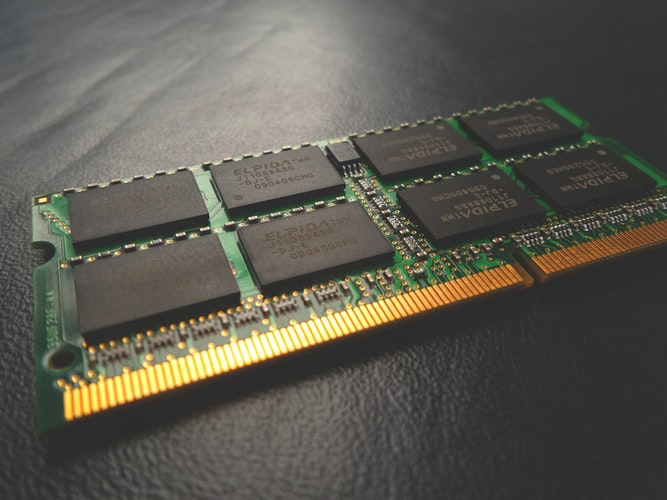
\includegraphics[width=\linewidth]{ram}
    \caption{RAM memory module}
    \label{img:ram}
\end{figure}

Here you can see a module of memory of a computer. This module is a circuit
board with memory chips soldered to it. The chips are the black rentangles.
In them it is stored
the information in binary code. A memory is a system from which you ask for a
portion of information and it deposits the value in a set of ``cables'' that
are in the computer, from which the values travel to the CPU, the processor,
the memory is \textbf{addressed}. This means that each portion of the memory
is referenced by a number.

Using an analogy, imagine that the memory is a notebook with a grid, in each
cell you can store a figure or a letter, to be able to fill or read the
cell, what we will do is assign a number to each one. We will start
with the number zero and after that the one, two...

\begin{table}[H]
    \centering
    \begin{tabular}{|c|c|c|c|c|c|c|c|c|c|c|c|c|c|c|}
        \hline
f&a&3&7&J&n&c&C&H&r&y&D&s&b&z\\\hline
a&y&y&4&c&B&W&D&x&S&2&2&J&j&z\\\hline
h&M&a&i&R&r&V&4&1&m&t&z&x&l&Y\\\hline
v&K&W&r&O&7&2&t&K&0&L&K&0&e&1\\\hline
z&L&O&Z&2&n&O&X&p&P&I&h&M&F&S\\\hline
v&8&k&P&0&7&U&2&0&o&0&J&9&0&x\\\hline
A&0&G&W&X&I&I&w&o&7&J&4&o&g&H\\\hline
F&Z&Q&x&w&Q&2&R&Q&0&D&R&J&K&R\\\hline
E&T&P&V&z&x&l&F&r&X&L&8&b&7&m\\\hline
t&K&L&H&I&G&h&I&h&5&J&u&W&c&F\\\hline
    \end{tabular}
    \caption{Example of a grid with values}
    \label{tab:notebookSimulation}
\end{table}

In the table you can see an emulation of this notebook, imagine that I tell
you ``tell me what is in the cell number 24''. Keeping in mind that it is
a table of 15 columns and that \textbf{we start counting from zero}, you'd have
to say ``S'', because the \textbf{address} 24 is the nineth position of the
second row. In general, computer memories are \textbf{addressed by bytes}, this
means that for each byte there is a number (an address). You may have noted that
it is absurd to draw this in a table if we are assigning simply numbers, this
should be a continous list, a table of a single column. If you have thought
that, you're right, because that's how memory is usually represented.

To sum it up: the memory in computers is a continous succession of bytes
numerated from zero and on, to which we can reference by that number
both to read and write.

\subsection{Positional numerical systems: decimal, binary, hexadecimal}
\label{numericSystems}
As we said in the introduction, the computer only understands binary code,
and this is applicable both to the addresses of the memory and its contents.
Due to this, I am compelled to teach you how the binary code works. The binary
code is a positional numerical system. In a positional system, numbers are
composed by figures, each one of those figures has a value depending on which
\textbf{position} they occupy in the number. The more to the left they are in
the number, the more they add to it. Remember when we learnt how numbers work,
you had units, tens, hundreds, thousands... and so on and so forth. The system
we use to write numbers is, therefore, positional, and decimal, because we have
ten figures (from zero to nine). In binary it's the same, but with only two
figures.

A positional numerical system works in this way: if the numeric base (number of
different figures available, in the case of our system, 10) is $n$, each figure
adds to the number the value of the figure multiplied by $n$ to the power of
how many figures remain to the right of this one. As always, let's see it with
and example: if we write the number 34,789, the calculation we perform to
know how much it adds up is this one (remember that any number that is not zero
powered to the zero power equals one):
$$
3\cdot10^4+4\cdot10^3+7\cdot10^2+8\cdot10^1+9\cdot10^0
$$
$$
3\cdot10000+4\cdot1000+7\cdot100+8\cdot10+9\cdot1
$$

Again, we can express it like tens, hundreds, units... which are the names
we have to those concrete powers of ten.

So, if you had a binary number, you'd make the same calculation, but instead of
unit, tens, hundreds and thousands, etc. you'd have to use units, couples,
quartets, octets and groups of 16 (there is no word for that). Given the binary
number 1110101, the calculation would be:
$$
1\cdot2^6+ 1\cdot2^5+1\cdot2^4+0\cdot2^3+1\cdot2^2+0\cdot2^1+1\cdot2^0
$$
$$
1\cdot64+ 1\cdot32+1\cdot16+0\cdot8+1\cdot4+0\cdot2+1\cdot1=117
$$

Now you already know how to read a binary number, you need to see how a decimal
number is converted to binary. To do so, you do the following:
\begin{enumerate}
\item Divide the number by two, calculating the residue.
\item If the division leaves no residue, you write a zero on the left side of
the resulting number, if it has residue (it can only be one), you write one.
\item Repeat until the \textbf{result} of the division is zero.
\end{enumerate}

Let's see an example of this, given the number 253, if you apply the procedure,
you should have something like the operations below. If you note the residues of
the divisions in the direction of the arrow in the bottom of the diagram you
could compose finally the binary number: 11111101.


$$
\matrix{
253                   &\division{2}                 &&&&&& \cr
\padding5\padding     &126                          &\division{2}                 &                      &                      &                             &                             &                             &                 \cr
\padding\underline{13}&\padding0\padding            &\padding63                   &\division{2}          &                      &                             &                             &                             &                 \cr
\padding\padding1     &\padding\padding\underline{6}&\padding0\padding            &\padding31            &\division{2}          &                             &                             &                             &                 \cr
                      &\padding\padding0            &\padding\padding\underline{3}&\padding1\padding     &\padding\underline{15}&\division{2}                 &                             &                             &                 \cr
                      &                             &\padding\padding 1           &\padding\underline{11}&\padding\padding1     &\padding\padding\underline{7}&\division{2}                 &                             &                 \cr
                      &                             &                             &\padding\padding1     &                      &\padding\padding1            &\padding\padding\underline{3}&\division{2}                 &                 \cr
                      &                             &                             &                      &                      &                             & \padding\padding1           &\padding\padding\underline{1}&\division{2}     \cr
                      &                             &                             &                      &                      &                             &                             & \padding\padding1           &\padding\padding0\cr
\padding\padding1     &\padding\padding0            &\padding\padding 1           &\padding\padding1     &\padding\padding1     &\padding\padding1            & \padding\padding1           & \padding\padding1           &                 \cr
}
$$
$$
\overleftarrow{\hphantom{\matrix{
		253                   &\division{2}                 &&&&&& \cr
		\padding5\padding     &126                          &\division{2}                 &                      &                      &                             &                             &                             &                 \cr
		\padding\underline{13}&\padding0\padding            &\padding63                   &\division{2}          &                      &                             &                             &                             &                 \cr
		\padding\padding1     &\padding\padding\underline{6}&\padding0\padding            &\padding31            &\division{2}          &                             &                             &                             &                 \cr
		&\padding\padding0            &\padding\padding\underline{3}&\padding1\padding     &\padding\underline{15}&\division{2}                 &                             &                             &                 \cr
		&                             &\padding\padding 1           &\padding\underline{11}&\padding\padding1     &\padding\padding\underline{7}&\division{2}                 &                             &                 \cr
		&                             &                             &\padding\padding1     &                      &\padding\padding1            &\padding\padding\underline{3}&\division{2}                 &                 \cr
		&                             &                             &                      &                      &                             & \padding\padding1           &\padding\padding\underline{1}&\division{2}     \cr
		&                             &                             &                      &                      &                             &                             & \padding\padding1           &\padding\padding0\cr
}}}
$$

If you are an user of computers, you may have heard sentences like
``this computer is a 32 bit computer'' or ``this computer is compatible with
64 bit software''. That numbers of bits is the size of, between other things,
the memory addresses. A computer of 32 bits has 32 bit memory addresses, hence
it can address 2\textsuperscript{32} bytes. Nowadays most computers are 64 bit,
so most of them can address 2\textsuperscript{64} bytes of information
theoretically. Of course, a computer will be always limited by the actual amount
of memory it has which, in normal computers, is usually around a handful of
gigabytes.

The problem is that 64 binary digits are too many to be read easily, look at
this binary number:
1101001001010101001010100101101010101010101110100100111010010101. It's too long.
Because of that, when memory addresses are written, they are written in a
different numerical system. This numerical system is the \textbf{hexadecimal}.
Is a system with base 16, with figures from zero to F. Yes, to F, you have read it
right. Since numbers in our normal system have base 10, we haven't got symbols
to represent a figure that has value 10, 11, 12... up to 15, so we use letter of
the latin alphabet. Otherwise, it works in the same way than binary or
decimal. A hexadecimal numbers is usually written with ``0x'' infront of it
to tell the reader that what follows is a number in that base. Let's see an
example, given the hexadecimal number 0xF2A.
$$
\mathrm{0xF2A} = 15\cdot16^2 + 2\cdot16^1 + 10\cdot16^0 = 3882
$$

To turn a decimal number into hexadecimal you must follow these steps:
\begin{enumerate}
\item Convert the number to binary
\item Divide the number in groups of four bytes \textbf{begining on the right
side}.
\item Turn each one of the groups to decimal and write the corresponding
hexadecimal digit.
\end{enumerate}

Let's go back to the example of the number we converted to binary before, 253,
in binary it is 11111101, if we wanted to convert it to hexadecimal we would
need to divide it in groups of four: 1111~1101. the number 1111 is 15, so it'd
be F, and the number 1101 is a 13, so it would be D, therefore 253 would be
equal to 0xFD. If the leftmost group is not a 4 byte group, you must put zeroes
on the left side. By the way, to convert from hexadecimal to binary, simply take
every hexadecimal digit and convert it to binary again but, remember, each
digit is a four byte binary number, so 0x33 would be 0011~0011. no 1111, that
would be a different number entirely. You're prepared to start learning how the
memory of a computer works.

\subsection{The memory map}
One of the most common ways to represent the memory of a computer is with a
\textbf{memory map}, that is a drawing it in the shape of a column in which the
contents of the memory are explained, indicating on the side the relevant
addresses. Look at the following figure:

\begin{figure}[H]
    \center
    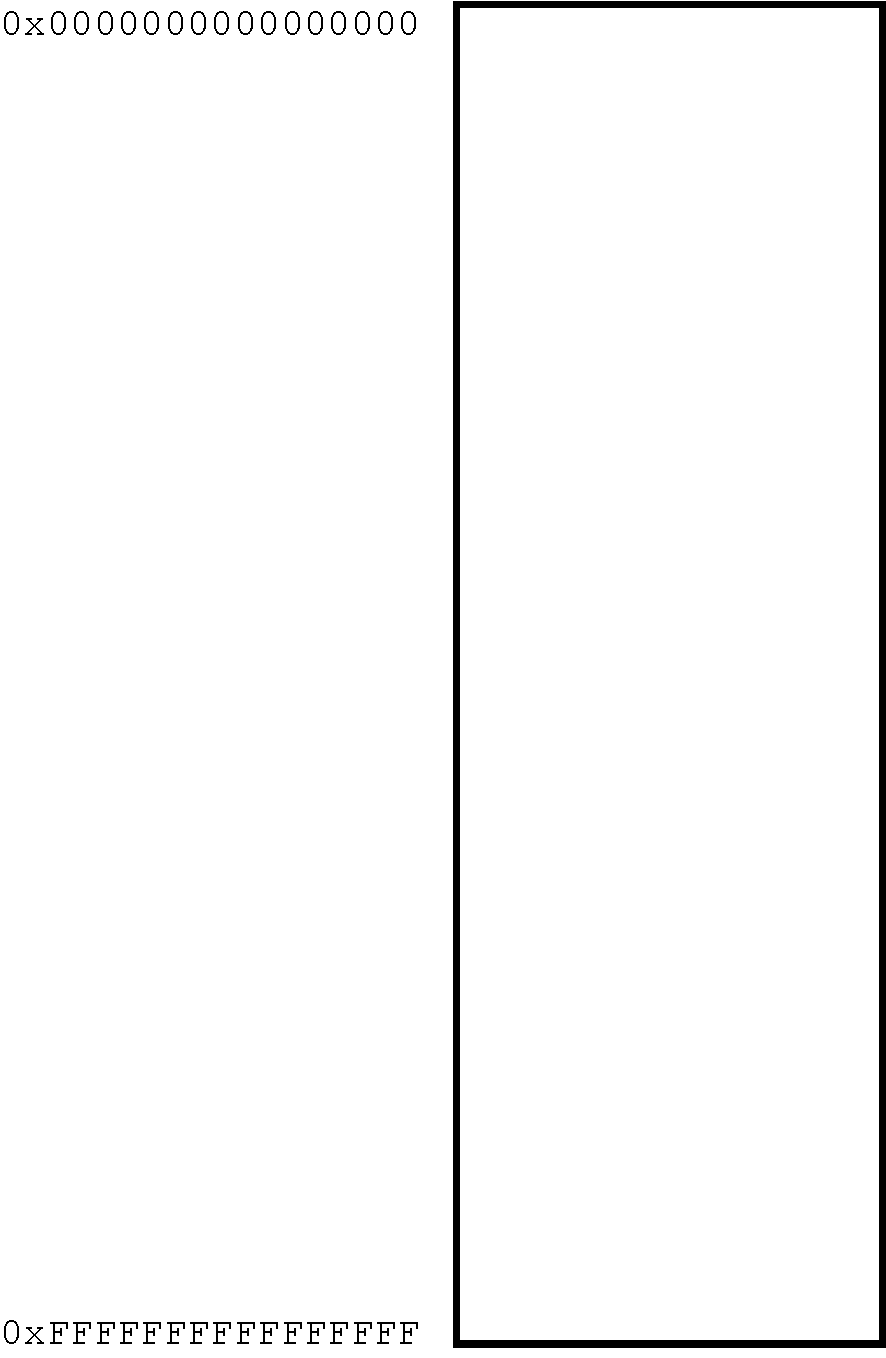
\includegraphics[width=0.5\linewidth]{emptyMemoryMap}
    \caption{Mapa de memoria vacío}
    \label{img:emptyMemoryMap}
\end{figure}

In that figure we have drawn the whole computer memory in a column, with
the lower addresses (near zero) in the top and the higher ones (closer to
0xFF...) in the bottom. Generally I like more this representation, but in
many sources and literature you'd see the map drawn in the other direction.

If your programs were the only software that executed in the computer, you'd
have the whole map available for you and you wouldn't have to do anything to
write on memory, simply... do it. But this is not the case, because your
programs are executed thanks to the operating system. The operating system has
many functionalities: it coordinates the programs that are executed in the
machine, manages file systems, allows the CPU to understand devices such as
keyboards and controllers... but one of its most basic functions is \textbf{
memory management}. First of all: when a program is executed, its contents are
loaded from where it is stored (your hard disk mainly) to your RAM memory, and a
\textbf{process} is created. A process is the actual program running in memory,
you could see the program as the blueprints of a car and the process as an
instance of a car, concrete, that is working in the world.
The OS gives processes memory blocks on which these can
write or not, and \textbf{ensures} that they do not go out of their assigned
memory.

In the section in which I talked about arrays I told you that if you accessed to
a position of an array that didn't exist, your program would end abruptly, test
it. Make a program that declares an array of, for example, 10 positions and
afterwards writes something in position 2,500. You'd see how the program writes
a message like this one when executed:

\noindent
\begin{minipage}[H]{\linewidth}
\mbox{}
\begin{lstlisting}[style=terminalStyle]
\$ ./main.exe
Segmentation fault (core dumped)
\end{lstlisting}
\end{minipage}

It is possible that it does not throw the message, due to how the computer
manages the memory internally. Anyway, for a C programmer, memory management
(and specially checking that he does not write to or reads from memory blocks he
shouldn't) is one of the most important tasks, if not the most. In this task,
the operating system decieves our programs. To our program, you have an
available memory that is the whole map (the 2\textsuperscript{64} bytes), even
when the computer may have, for example, 8~GB which is several thousand times
less. By the way, in general terms, each level in the prefixes of multiplication
of 1,000 is not 1,000, but 2\textsuperscript{10}, 1,024, when you're talking
about bytes, if we were exhaustive,
we should write GiB, MiB and so on, which is the correct way to indicate those
prefixes that multiply by 1,024. What the operating system does is to allocate
what we ask from it in the \textbf{physical} memory and gives us addresses of
that map of memory we think we have, and translates it. This process is the
\textbf{memory virtualization}, and is one of the most important features of an
operating system. Thanks to it, the programmer doesn't need to manage where the
memory is physically allocated. Also, it allows each process to be isolated,
the programmer has no idea which other processes are doing in their memory map,
and other processes have no information about what we're doing with ours.

In this map of virtualized memory, which is efectivelly the one we're going to
use, the operating system creates a set of \textbf{memory regions}, which are
used to alocate different types of information of each process executing in a
computer.
Now I will show you a memory map with the most important regions, and I will
explain what they are and why we care about them.
\begin{figure}[H]
    \center
    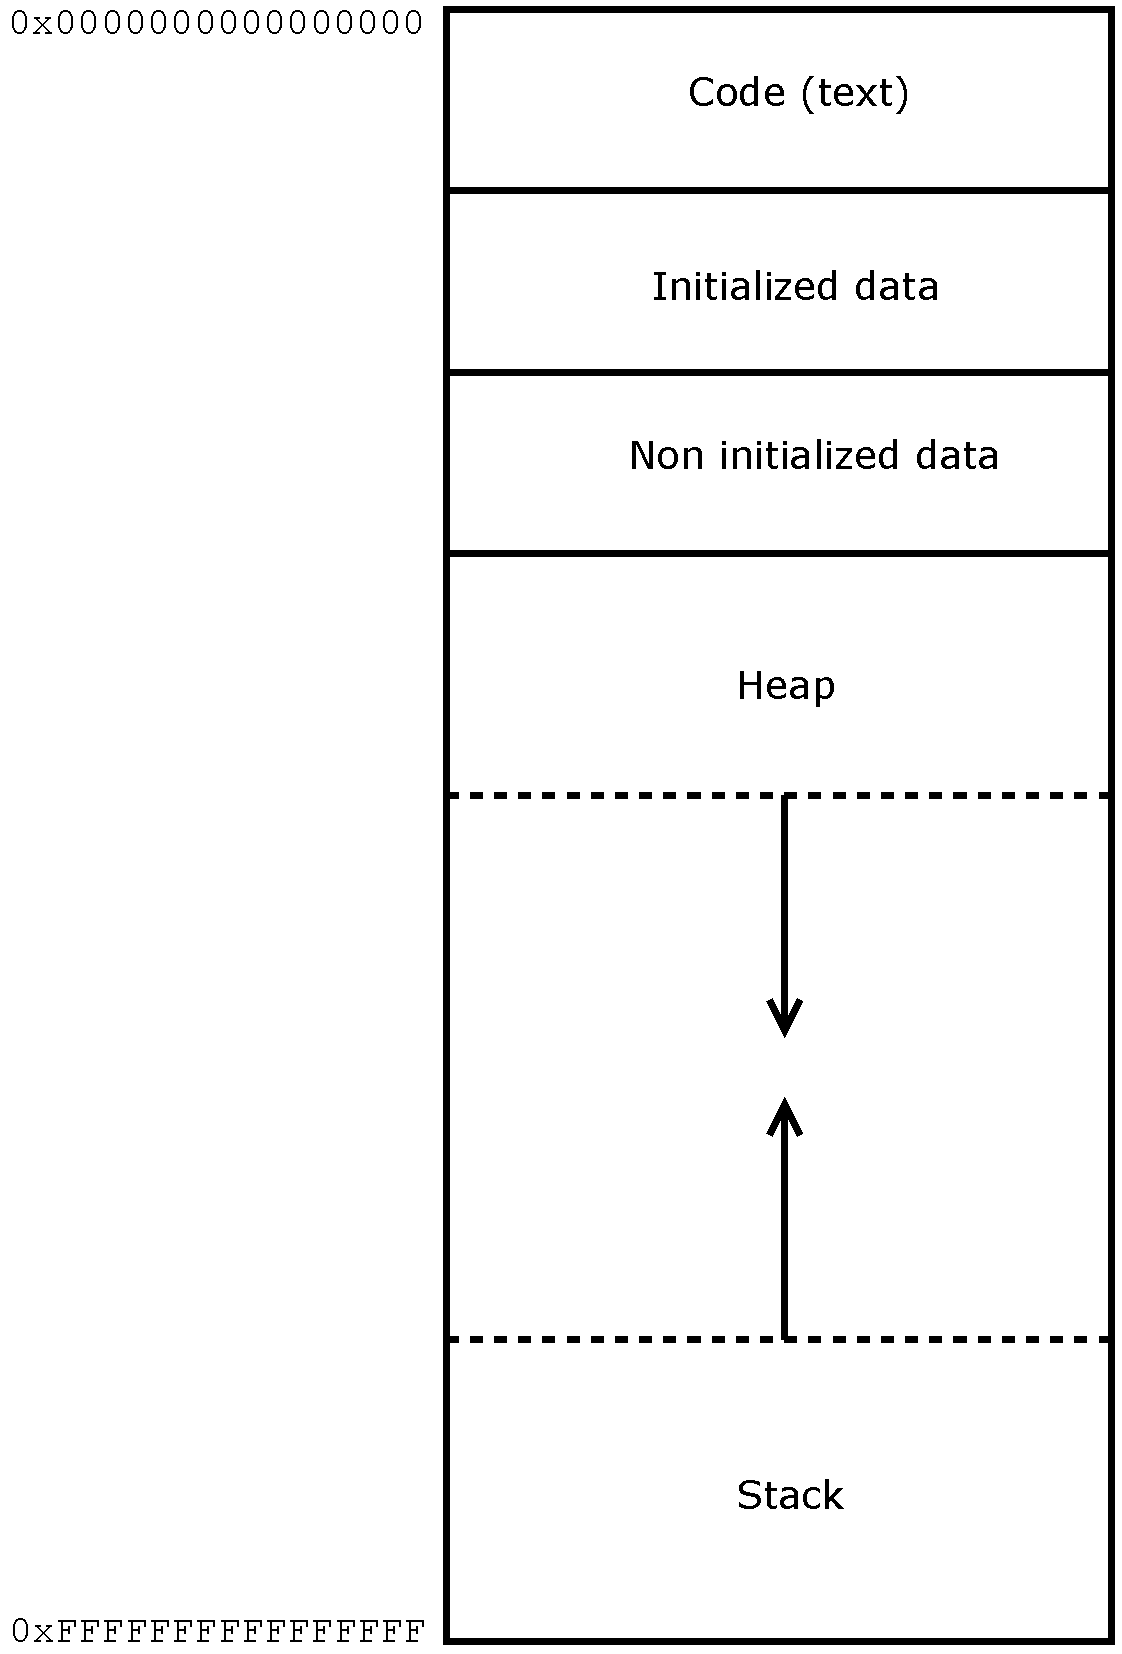
\includegraphics[width=0.5\linewidth]{regionsMemoryMap_en}
    \caption{Regions of the memory map of a process}
    \label{img:regionsMemoryMap}
\end{figure}

The text region is easy, it is were the instructions that your program is going
to execute are stored. When I explained you what compilation was I told you we
were going to transform our instructions into a binary the computer can execute.
This is the section where it is stored. To generate a program, those
instructions in binary are stored in the disk in the executable. When they load
in memory, they go in this section. This section can't be directly read or
changed by the program itself.

The next one starts to be interesting. This sections stores the value of the
global variables, either of basic types, arrays, or structs that you write
initialized in the code (initializing the variables from a function or other
block of code won't count). This is because the values you store in them will
exist before your program starts executing, in the very moment the process is
created. The next section stores those \textbf{global} variables you haven't
initialized. Why only the global ones in both cases? Because the function
\verb!main! is a function and the variables declared in functions (or any other
block of code) are not stored here, but in the next section, the stack.

Look at the map, this section is at the bottom (towards the higher addresses),
but I am going to explain it now because it is one of the most important. The
variables you declare in a block of code: functions, loops, conditionals, etc.
are stored. Why? Because in this section of memory data can go in and out, or
better said, the memory of old data can be reused to write new ones. To explain
how this is done, firstly I need to explain you how a stack (in general terms)
works.

A stack is a data structure, like arrays or structs, which works in this way:
when you put something in the stack, that element is on top, and when you pull
out something from the stack, you can only pull out the last element, the one
in the top of the stack. I am going to set a physical example: a can of the
famous Pringles\textsuperscript{®} potato chips. The only chip that you can
pull out is the top one, if you want get more, you can, but always in the
reverse order from how they were put in the can. Any stack works the same. The
way this stack is applied to C programming is this way: when the execution flow
goes into any code block, the variables declared inside it are \textbf{added}
to the stack. This includes arrays and structs. When the flow goes out of the
block, those variables are \textbf{pulled out} of the stack, that is, they're
lost because it is understood they were already used. This is the very reason
\textbf{functions cannot return arrays}. Because those array would cease
existing once the function has returned.

Maybe you're wondering why you can declare basic types variables or structs
inside functions and return them, if they're going to be destroyed once the
function is finished executing. That is because, in the same way the arguments,
the return value when it is not an array gets copied. Concretely is left in the
top part of the stack so the \textbf{code which called} the function can
copy it with an assignation. With array \textbf{we cannot use the assignment
operator}, it is not how arrays are copied. As a matter of fact the compiler
would throw an error if you tried assigning an array to another.

Let's see an example of how the stack would look in the case of executing some
of the example programs we've written. We're going to use the program
\ref{lst:arraysAndFunctions}: \nameref{lst:arraysAndFunctions}.
In this example you're going to see that in the stack there two names
(\verb!my_array! and \verb!array!), but remember they \textbf{point to the same
array}. They only copy the address it starts in, not the elements.
\begin{table}[H]
\centering
    \begin{subfigure}{0.33333\linewidth}
        \centering
        \begin{tabularx}{.9\linewidth}{|Y|}
        \hline
        \textbf{The stack starts empty}\\\hline
         \\\hline
        \multicolumn{1}{c}{\color{white}CIERTOFALSO\normalcolor}\\ \arrayrulecolor{white}\hline
        \multicolumn{1}{c}{\color{white}CIERTOFALSO\normalcolor}\\ \arrayrulecolor{white}\hline
        \multicolumn{1}{c}{\color{white}CIERTOFALSO\normalcolor}\\ \arrayrulecolor{white}\hline
        \end{tabularx}
    \end{subfigure}%
    \begin{subfigure}{0.33333\linewidth}
        \centering
        \begin{tabularx}{.9\linewidth}{|Y|}
        \hline
        \textbf{Going into \texttt{main}}\\\hline
        my\_array\\\hline
        \multicolumn{1}{c}{\color{white}CIERTOFALSO\normalcolor}\\ \arrayrulecolor{white}\hline
        \multicolumn{1}{c}{\color{white}CIERTOFALSO\normalcolor}\\ \arrayrulecolor{white}\hline
        \multicolumn{1}{c}{\color{white}CIERTOFALSO\normalcolor}\\ \arrayrulecolor{white}\hline
        \end{tabularx}
    \end{subfigure}%
    \begin{subfigure}{0.33333\linewidth}
        \centering
        \begin{tabularx}{.9\linewidth}{|Y|}
        \hline
        \textbf{Going into \texttt{print\_array}}\\\hline
        array\\\hline
        array\_size\\\hline
        my\_array\\\hline
        \multicolumn{1}{c}{\color{white}CIERTOFALSO\normalcolor}\\ \arrayrulecolor{white}\hline
        \end{tabularx}
    \end{subfigure}%


    \begin{subfigure}{0.33333\linewidth}
        \centering
        \begin{tabularx}{.9\linewidth}{|Y|}
        \hline
        \textbf{Going into \texttt{for}}\\\hline
        ii \\\hline
        array\\\hline
        array\_size\\\hline
        my\_array\\\hline
        \multicolumn{1}{c}{\color{white}CIERTOFALSO\normalcolor}\\ \arrayrulecolor{white}\hline
        \end{tabularx}
    \end{subfigure}%
    \begin{subfigure}{0.33333\linewidth}
        \centering
        \begin{tabularx}{.9\linewidth}{|Y|}
        \hline
        \textbf{We exit the \texttt{for}}\\\hline
        array\\\hline
        array\_size\\\hline
        my\_array\\\hline
        \multicolumn{1}{c}{\color{white}CIERTOFALSO\normalcolor}\\ \arrayrulecolor{white}\hline
        \multicolumn{1}{c}{\color{white}CIERTOFALSO\normalcolor}\\ \arrayrulecolor{white}\hline
        \end{tabularx}
    \end{subfigure}%
    \begin{subfigure}{0.33333\linewidth}
        \centering
        \begin{tabularx}{.9\linewidth}{|Y|}
        \hline
        \textbf{We exit \texttt{print\_array}} \\\hline
        my\_array\\\hline
        \multicolumn{1}{c}{\color{white}CIERTOFALSO\normalcolor}\\ \arrayrulecolor{white}\hline
        \multicolumn{1}{c}{\color{white}CIERTOFALSO\normalcolor}\\ \arrayrulecolor{white}\hline
        \multicolumn{1}{c}{\color{white}CIERTOFALSO\normalcolor}\\ \arrayrulecolor{white}\hline
        \multicolumn{1}{c}{\color{white}CIERTOFALSO\normalcolor}\\ \arrayrulecolor{white}\hline
        \end{tabularx}
    \end{subfigure}%

    \begin{subfigure}{0.4\linewidth}
        \centering
        \begin{tabularx}{.9\linewidth}{|Y|}
        \hline
        \textbf{Going into \texttt{add\_one\_to\_each}} \\\hline
        array\\\hline
        array\_size\\\hline
        my\_array\\\hline
        \multicolumn{1}{c}{\color{white}CIERTOFALSO\normalcolor}\\ \arrayrulecolor{white}\hline
        \multicolumn{1}{c}{\color{white}CIERTOFALSO\normalcolor}\\ \arrayrulecolor{white}\hline
        \end{tabularx}
    \end{subfigure}%
    \begin{subfigure}{0.2\linewidth}
        \centering
        \begin{tabularx}{\linewidth}{|Y|}
        \hline
        \textbf{Going into \texttt{for}} \\\hline
        ii\\\hline
        array\\\hline
        array\_size\\\hline
        my\_array\\\hline
        \multicolumn{1}{c}{\color{white}CIERTOFALSO\normalcolor}\\ \arrayrulecolor{white}\hline
        \end{tabularx}
    \end{subfigure}%
    \begin{subfigure}{0.4\linewidth}
        \centering
        \begin{tabularx}{.9\linewidth}{|Y|}
        \hline
        \textbf{We exit the \texttt{for}}\\\hline
        array\\\hline
        array\_size\\\hline
        my\_array\\\hline
        \multicolumn{1}{c}{\color{white}CIERTOFALSO\normalcolor}\\ \arrayrulecolor{white}\hline
        \multicolumn{1}{c}{\color{white}CIERTOFALSO\normalcolor}\\ \arrayrulecolor{white}\hline
        \end{tabularx}
    \end{subfigure}%


    \begin{subfigure}{0.33333\linewidth}
        \centering
        \begin{tabularx}{.9\linewidth}{|Y|}
        \hline
        \textbf{We exit \texttt{add\_one\_to\_each}} \\\hline
        my\_array\\\hline
        \multicolumn{1}{c}{\color{white}CIERTOFALSO\normalcolor}\\ \arrayrulecolor{white}\hline
        \multicolumn{1}{c}{\color{white}CIERTOFALSO\normalcolor}\\ \arrayrulecolor{white}\hline
        \multicolumn{1}{c}{\color{white}CIERTOFALSO\normalcolor}\\ \arrayrulecolor{white}\hline
        \multicolumn{1}{c}{\color{white}CIERTOFALSO\normalcolor}\\ \arrayrulecolor{white}\hline
        \end{tabularx}
    \end{subfigure}%
    \begin{subfigure}{0.33333\linewidth}
        \centering
        \begin{tabularx}{.9\linewidth}{|Y|}
        \hline
        \textbf{Going into \texttt{print\_array}}\\\hline
        array\\\hline
        array\_size\\\hline
        my\_array\\\hline
        \multicolumn{1}{c}{\color{white}CIERTOFALSO\normalcolor}\\ \arrayrulecolor{white}\hline
        \multicolumn{1}{c}{\color{white}CIERTOFALSO\normalcolor}\\ \arrayrulecolor{white}\hline
        \end{tabularx}
    \end{subfigure}%
    \begin{subfigure}{0.33333\linewidth}
        \centering
        \begin{tabularx}{.9\linewidth}{|Y|}
        \hline
        \textbf{Going into the \texttt{for}}\\\hline
        ii \\\hline
        array\\\hline
        array\_size\\\hline
        my\_array\\\hline
        \multicolumn{1}{c}{\color{white}CIERTOFALSO\normalcolor}\\ \arrayrulecolor{white}\hline
        \end{tabularx}
    \end{subfigure}%


    \begin{subfigure}{0.33333\linewidth}
        \centering
        \begin{tabularx}{.9\linewidth}{|Y|}
        \hline
        \textbf{We exit the \texttt{for}}\\\hline
        array\\\hline
        array\_size\\\hline
        my\_array\\\hline
        \multicolumn{1}{c}{\color{white}CIERTOFALSO\normalcolor}\\ \arrayrulecolor{white}\hline
        \end{tabularx}
    \end{subfigure}%
    \begin{subfigure}{0.33333\linewidth}
        \centering
        \begin{tabularx}{.9\linewidth}{|Y|}
        \hline
        \textbf{We exit \texttt{print\_array}} \\\hline
        my\_array\\\hline
        \multicolumn{1}{c}{\color{white}CIERTOFALSO\normalcolor}\\ \arrayrulecolor{white}\hline
        \multicolumn{1}{c}{\color{white}CIERTOFALSO\normalcolor}\\ \arrayrulecolor{white}\hline
        \multicolumn{1}{c}{\color{white}CIERTOFALSO\normalcolor}\\ \arrayrulecolor{white}\hline
        \end{tabularx}
    \end{subfigure}%
    \begin{subfigure}{0.33333\linewidth}
        \centering
        \begin{tabularx}{.9\linewidth}{|Y|}
        \hline
        \textbf{We exit \texttt{main}} \\\hline
        \\\hline
        \multicolumn{1}{c}{\color{white}CIERTOFALSO\normalcolor}\\ \arrayrulecolor{white}\hline
        \multicolumn{1}{c}{\color{white}CIERTOFALSO\normalcolor}\\ \arrayrulecolor{white}\hline
        \multicolumn{1}{c}{\color{white}CIERTOFALSO\normalcolor}\\ \arrayrulecolor{white}\hline
        \end{tabularx}
    \end{subfigure}%
\caption{Example of the state of the stack in an execution}
\label{tab:stackExample}
\end{table}

Now you know how the stack works and the implications it has in the arrays
saved in it, we can see the last region and maybe the most important, the heap.
This region stores the memory you ask for from the operating system using a series of
functions we're going to see. And you may be thinking: why would you do that if
you can declare an array? Simple, this memory you ask the operating system for
is always available to you \textbf{until you free it}. That means that,
contrary to the arrays, it's your duty to worry about freeing it. Is one of the
most important tasks of a C programmer, but to do so, you need to learn first
what pointers are.

\subsection{Pointers}
Now you know that the memory is addressed by bytes, you must know how we use
addresses in the C language. We do it with a new type (for us) called pointer.
A pointer is a variable that stores a memory address, and allow us to
communicate to functions or other parts of the program \textbf{a memory block}.
You have already used pointers, but you didn't know what they were because I
have chosen to explain other things first, although I have been anticipating
its use.

I told you before that when a function receives an array as an argument it
decays to a mere pointer. This means we do not copy the arrays functions
receive, what we do is tell the function where the elements of the array are in
memory. In this way, if it is necessary to perform a copy, we can do it, if
not, the function can chose to manipulate or read them directly.

If a pointer symbolizes a memory address, you can think only one type for memory
addresses is needed, but this is not the case. Each datatype (either basic or
struct) has its own pointer, that is, there are not only pointers, but pointers
to \texttt{double}, \verb!char!, to this or that struct... Why is that? Because
when using pointers with associated types, we know \textbf{what is} in the
memory the address points to. For example, if we have a pointer to \verb!int!
that is 0xFB455DE, we know we must take that byte and the three next ones and
decode them as an integer. Let's see it in the code.

\noindent
\begin{minipage}[H]{\linewidth}
\mbox{}
\begin{lstlisting}[style=C, label={lst:pointers1},
caption={Pointer declaration}]
#include <stdio.h>

int main(void)
{
    int a = 2;
    int *ptr_to_a;
    ptr_to_a = &a;
    printf("a is in address %p and it is %d\n", ptr_to_a, a);
}
\end{lstlisting}
\end{minipage}

In line 7 we declare a pointer variable for the first time, this is done with
an asterisk that you see between the type of the variable and the name. This is
where it is stablished that this pointer is associated to an \texttt{int}. In
the next line we're assigning to this pointer the value of the address where
\verb!a! is located. We use the operator \verb!&!. The name of the operator
is ampersand. Said operator, infront of an expression, gives us the pointer to
its type with the address said expression is stored in. Mind that, for this to
work, this expression must be stored somewhere. That is, the temporal values
would throw an error, for example: \verb!&(a * 2)! would throw an error, because
\verb!a*2! hasn't been stored in any place. If you execute the program that uses
the pointer, the output will be something like this:

\noindent
\begin{minipage}[H]{\linewidth}
\mbox{}
\begin{lstlisting}[style=terminalStyle]
\$ ./main.exe
a is in address 0x7fffde738b6c and it is 2
\end{lstlisting}
\end{minipage}

Then, let's see a practical case of what pointers are useful for, for example:
we have said several times that a function receives a copy of the arguments but,
what if we wanted to save that effort? If, for example, you wanted a function
that multiplies a number by another, maybe you do not want to copy it, the
function returning the result and copying that result again in the variable,
simply \textbf{leave the function work for you}. If we pass the pointer to our
variable the function will be the one changing the value, let's see it.

\noindent
\begin{minipage}[H]{\linewidth}
\mbox{}
\begin{lstlisting}[style=C, label={lst:pointers1},
caption={Pointer ussage example}]
#include <stdio.h>
void multiply(int* ptr, int b) {
    (*ptr) *= b;
}
int main(void)
{
    int a = 2;
    int* pointer_to_a;
    pointer_to_a = &a;
    printf("a is in address %p and it is %d\n", pointer_to_a, a);
    multiply(pointer_to_a, 4);
    printf("a is in address %p and it is %d\n", pointer_to_a, a);
}
\end{lstlisting}
\end{minipage}

Here you can see you we declare a function that received a pointer to integer
(the variable we want to multiply) and an integer (the number we want it to
be multiplied by). In this function you'd see a new use of the asterisk
operator, (\verb!*!), which is the one for \textbf{dereferencing} a pointer.
What is that? It is accessing the value that pointer is referencing (hence the
name). Remember that, as a pointer, \verb!ptr! stores the memory address, so we
need a way to tell C to store in that address the multiplied number. To do so,
we use the asterisk before the pointer. In simple words, the asterisk turns the
\verb!int*! into the \verb!int! that pointer points to. It ``follows the
pointer''. After that, we use the operator
\verb!*=! to multiply and assign. In line 11 you see how we simply call the
function, without having to store what it returns (in fact, we have defined it
as \verb!void! so it does not return anything) and we avoid copying the integer
we wanted to multiply.

Apart from the asterisk operator, there is another operator that is used with
pointers that you must know, this is the arrow opeator \verb!->!. It is used to
access the fields of a pointer to a struct. This may be a little confusing, but
I am going to take my time. Imagine we have the point struct we wrote in the
section about structs. If, for any reason, we were using a pointer to it and
wanted to access its fields, we should use the operator asterisk to dereference
the pointer and then the operator dot to access the field. For example, let
\verb!point_ptr! be a pointer to \verb!struct point_s!, to access its value
\verb!x!, we had to write \verb!(*point_ptr).x!. It is not a problem, but I warn
you that it is very common to have structs with pointers to other structs and so
on... it can become pretty illegible in three or four times. That is why we have
the arrow operator, to make that earlier code turn into simply:
\verb!point_ptr->x!. I want to clarify that this operator accesses to the field,
does not gives us a pointer to said field. That is, following the example,
\verb!point_ptr->x! would be a \verb!double!, not a \verb!double*!. Later on we
will see this operator in real use.

\subsubsection{Pointer arithmetic}
Arrays are in certain aspect (but \textbf{not} all) equivalent to pointers, due
to this, pointers can be dereferenced with the square bracket operator. As a
matter of fact, you can turn an array into a pointer explicitly in your program.
As always, let's see how it is done:

\noindent
\begin{minipage}[H]{\linewidth}
\mbox{}
\begin{lstlisting}[style=C, label={lst:pointers2},
caption={Arrays as pointers}]
#include <stdio.h>

int main(void)
{
    int my_array[10] = {0,1,2,3,4,5,6,7,8,9};
    int* pointer_like_array = my_array;
    for (int ii = 0; ii < 10; ++ii) {
        printf("array[%d] = %d\n", ii, my_array[ii]);
    }
    puts("========");
    for (int ii = 0; ii < 10; ++ii) {
        printf("array[%d] = %d\n", ii, pointer_like_array[ii]);
    }
}
\end{lstlisting}
\end{minipage}

What you see in the program \ref{lst:pointers2} is what happens without
you noticing it when a function receives an array, it's turned into a pointer
and you can use it with the same operators of an array. This, nevertheless; is
only valid for one dimension array, for a reason we will see later on.
Exhaustively speaking, the square brackets operator is a \emph{shortcut}. Actually
what it does is add to the pointer and use the asterisk to dereference. When you
add an integer type to a pointer, the pointer arithmetic starts to play, let's
see an example and I'll show you how it works.

\noindent
\begin{minipage}[H]{\linewidth}
\mbox{}
\begin{lstlisting}[style=C, label={lst:pointers3},
caption={Aritmética de punteros}]
#include <stdio.h>

int main(void)
{
    int my_array[10] = { 0,1,2,3,4,5,6,7,8,9 };
    int* pointer_like_array = my_array;
    for (int ii = 0; ii < 10; ++ii) {
        printf("In address %p there is a %d\n",
            pointer_like_array + ii,
            *(pointer_like_array + ii));
    }

}
\end{lstlisting}
\end{minipage}

If you execute the program you would see that the addresses are four units
apart. This is because when you add an integer to a pointer, even when said
pointer is a memory address of a memory addressed by bytes, due to being a
pointer to \textbf{integer}, that expression of adding an integer to it is
translated into adding the integer multiplied by the size of an \verb!int!
(four bytes). After this, we use the asterisk operator so this pointer we have
added a number is dereferenced. Using pointer arithmetic is useful when
you want to pass to a function the pointer of a position of an array. For
example:

\noindent
\begin{minipage}[H]{\linewidth}
\mbox{}
\begin{lstlisting}[style=C, label={lst:pointers4},
caption={Practical example of pointer arithmetic}]
#include <stdio.h>
void multiply(int* number, int other) {
    *number *= other;
}

void multiply_array(int* array, int array_length, int other) {
    for (int ii = 0; ii < array_length; ++ii) {
        multiply(array + ii, other);
    }
}

void print_array(int array[], int array_size) {
    for (int ii = 0; ii < array_size; ++ii) {
        printf(" %d ", array[ii]);
    }
    printf("\n");
}

int main(void)
{
    int array[] = { 1,2,3,4,5,6,7,8,9,10 };
    print_array(array, 10);
    multiply_array(array, 10, 10);
    print_array(array, 10);
}
\end{lstlisting}
\end{minipage}

%%%%%%%%%%%%%%%%%%%%%%%%%%%%%%%%%%%%%%%%%%%%%%%%%%%%%%%%%%%%%%%%%%%%%%%%%%%%%
As an instance, if we use the function that multiplies a number without having
to return it, we can write a function that does the same with an array (here
you can appreciate how functions are a way to reuse code and avoid duplicating
it). We can also see how, using pointer arithmetic, you do not need to have into
account the size of each data type, the language does it for you. There is an
alternative way to do this that you may see because it is more compact, and it
is using the square brackets operator to get the element and then use the
ampersand to retrieve the address, doing so, line 8 would turn into
\lstinline[style=C]{multiply(&array[ii], other);}. In those cases, using one
or the other is choice of the programmer.

\subsubsection{The \texttt{char} pointer}
Finally I am going to unveil uno of the misteries that I have been hiding from
you for the most time (against my will, for the record) about the programs we
have written up until now. This mistery is: what are those texts between double
quotes, for example: \verb!"Hello, world!"!. I got a bit ahead of myself in the
title because I wrote the answer there, but they're an abbreviated way to write
\textbf{arrays of \texttt{char}}. You know that a \verb!char! is a letter, and
that an array is a succession of data. The logic conclusion is that, in C, texts
are \verb!char! arrays. If they're \verb!char! arrays, where is their
declaration and why are they there between quotes. To sum it up: because we
write texts in our program so often, the creators of C decided to add a
\textbf{constant expression} to be able to declare arrays of \verb!char!
where it is needed, this expression is putting the text in quotes.
There are expressions to declare arrys of other types, but they're not so
important so we will see them in later sections.

Nevertheless; there is a differente between a \verb!char! array (or pointer when
it is passed to a function) and an array of another data type. The function
\verb!printf!, but in any place we say the size of the array, the number of
elements on the memory the pointer points to. The functions that receive it must
have some mechanism to know how many there are. That way is that every text
chain (called strings in programming) in C finishes in a \verb!char! with
value zero. That is, when it is written \verb|"Hola, mundo!"| we are creating
in a quick way an array of \verb!char! that contains \textbf{fourteen}
\verb!char!, the letters you can see and a \verb!char! with value zero at the
end. I am going to demonstrate this is the case with a little program:

\noindent
\begin{minipage}[H]{\linewidth}
\mbox{}
\begin{lstlisting}[style=C, label={lst:sizeofArraysPointers}, caption={Charr array}]
#include <stdio.h>

int main(void)
{
    char correct_string[] = "I like choccy milk.\n";
    char incorrect_string[] = {'I', ' ', 'l', 'i', 'k', 'e', ' ',
                               'c', 'h', 'o', 'c', 'c', 'y', ' ',
                               'm', 'i', 'l', 'k', '.', '\n'};
    printf(correct_string);
    printf(incorrect_string);
}
\end{lstlisting}
\end{minipage}

The first string will be printed correctly, but the second will print and,
with all probability, after it, other characters will be printed, probably
nonsense (execute the program a couple times, it may work well the first time).
This is because since the second string is not ended in a char with
value \verb!zero!, \verb!printf! doesn't know where to stop printing. Aside from
this way of working with them, \verb!char! arrays work like any other array and,
when they're turned into pointers, like any other pointer. In later sections
I will show how to manipulate text strings in more advanced ways.
\subsubsection{The null pointer}
There is an special value for all the types of pointer, which is the null
pointer, or, as it is written in the language: \verb!NULL!. It is a \verb!void!
pointer that is equal to zero. If you remember, the memory map that address
would correspond to the text section, our program can't modify itself or read
the binary instructions, among other things because part of that section is not
our code, but the code of operating system which inserts itself in processes to
allow us to do certain things. Hence the designers of the language used this
value to symbolize a pointer that is in a special state.

One of the most important uses of this pointer is that it is used to express if
an operation has gone well or not. For example, when we open a file with a
function called \verb!fopen!, this returns a pointer to a struct, if the file
does not exist, or the program hasn't got permissions to open it, the pointer
will be \verb"NULL". Many functions that receive a pointer use \verb!NULL! to
express an special behaviour. For ecample, let's write a function that
encapsulates the functionality of the program \ref{lst:pointNoStruct}, this has
been an exercise, so if you didn't do it yet, do it now; but we're going to
give it a twist: instead of receiving the structs, let's receive pointer to the
structs. First, because as I said you, we save ourselves copying the structs and
we can use \verb!NULL! to indicate special values.

\noindent
\begin{minipage}[H]{\linewidth}
\mbox{}
\begin{lstlisting}[style=C, label={lst:nullPointers},
caption={Use of pointers to \texttt{NULL}}]
struct point_s {
    double x; double y;
};

double distance(struct point_s *a, struct point_s *b) {
    double res = 0.0;
    struct point_s origin = { .x = 0.0, .y = 0.0 };
    if(NULL == a){
        a = &origin;
    }
    if(NULL == b){
        b = &origin;
    }
    double diff_x = a->x - b->x;
    double diff_y = a->y - b->y;
    res = sqrt(diff_x * diff_x + diff_y * diff_y);
    return res;
}

int main(void)
{
    struct point_s a = {.x = 3, .y = 4};
    double d = distance(&a, NULL);
    printf("Distance: %f\n", d);
}
\end{lstlisting}
\end{minipage}

If you look at the function we have written, inside it we declare a point that
symbolizes the \textbf{origin of coordinates}. What we do is that if one of the
pointers to the structs is \verb!NULL!, we understand that such point is
the origin of coordinates. What we do is assigning to our arguments (which
are pointers) the address to this local variable we have declared. Remember:
the arguments that a function receives are \textbf{copies} of the values. In
this case, our argument is a pointer to a struct. Assigning to our argument
other value \textbf{we are not altering the original structure}, because we
haven't changed the value our argument points to, but the argument itself. Once
this is done, we can calculate the distance in the same way we would do if they
weren't pointers. What is the use of writing a function in this way? Finding
the distance to the origin of coordinates is a common operation, doing things
this way, we allow the program to call the function to do such calculation
without declaring an extra struct to symbolize the origin.

\subsection{Allocate and free memory}
Now we have learnt what a pointer is, and to manage them, we can ask the
operating system for memory of the kind that is stored in the heap and we can
manage in a more flexible way than arrays. To do so we use two functions:
\verb!malloc! and \verb!free!. The names of the functions are very descriptive,
the first means ``memory alloc'' and the second frees the memory. When you need
to reserve memory in the heap, you call \texttt{malloc} and ask for a contiguous
memory block of $n$ bytes. The function \verb!malloc! returns a \verb!void!
pointer. That same pointer should, at some time, be freed passing it to
\texttt{free}.

Talking about pointers to \verb!void!, I told you that \verb!void! means that
the functions either don't receive anything or don't return anything. The
meaning of a \verb!void! pointer is related to that: it is a pointer that you do
not know what it is, \verb!malloc! has no way to know what you are going to do
with the memory, therefore it returns a \verb!void! pointer. A pointer to
\verb!void! is also useful when we want to write functions or structs that are
compatible with different data types. Let's see first a simple example on how to
use \verb!malloc! and \verb!free!.

One of the advantages of dynamic memory allocation occurs when other part of
the program performs a calculation whose result has an unknown size. For
example, imagine a function that, given an array of number, returns a vector
with an instance of every distinct number, that is, erases repetitions, let's
call it \verb!erase_reps!. Functions cannot return arrays, that's something we
already know, but the person that calls \verb!erase_reps! could declare an array
and pass it to the function, a problem arises nevertheless: we do not know
the size that array will have. Is it true that we have an \textbf{upper bound},
if we give to this function an array of $n$ positions, the result can only have,
at most, $n$ positions. So we could declare an array of $n$ positions
and tell the function to leave there the results. But there is a problem, how do
we know which part is solution and wich part is excess? The only thing you could
so is to return from \verb!erase_packets! the size of the solution. In this case
you'd have to an array of $n$ positions of which you'd use a lesser amount.
You'd be wasting memory and, even when it does not look like a problem, it may
become one very quickly.

\noindent
\begin{minipage}[H]{\linewidth}
\mbox{}
\begin{lstlisting}[style=C, label={lst:mallocAndFree},
caption={Example of dynamic allocation}]
#include <stdio.h>
#include <stdlib.h>

int *erase_reps(int* array, int array_length, int* final_length) {
    *final_length = 0;
    int preliminary_array[array_length];
    for (int ii = 0; ii < array_length; ++ii) {
        int unique = 1;
        for (int jj = 0; jj < ii; ++jj) {
            if (array[ii] == array[jj]) {
                unique = 0;
                break;
            }
        }
        if (unique) {
            preliminary_array[*final_length] = array[ii];
            ++(*final_length);
        }
    }

    int* result = malloc(*final_length * sizeof(int));

    for (int ii = 0; ii < *final_length; ++ii) {
        result[ii] = preliminary_array[ii];
    }
    return result;
}


int main(void)
{
    int array[] = { 20,1,2,3,4,5,8,7,8,9,6,6,5,4,1,2,3,8,5,4,4,5,6};
    int length;
    int* result = erase_reps(array, 23, &length);
    for (int ii = 0; ii < length; ++ii) {
        printf("%d\n", result[ii]);
    }
    free(result);
}
\end{lstlisting}
\end{minipage}

In the line 2 of code we see how the line \verb!#include <stdlib.h>! makes its
appearance, it is needed to use \verb!malloc! and \verb!free!. After it we have
the declaration of the function, we have made it return the pointer to the
result and receive three arguments: the array from which we're erasing
repetitions, the length of such array and a pointer to integer that will allow
us to \textbf{indicate the length of the solution}. This pattern is very used in
C programs, when you need the function to calculate a lot of things, you receive
pointers to those things and write the results there. In the body of the
function we assign 0 to \verb!final_length! to start. After it, we declare a
preliminar array to save the unique numbers, why an array? Because this is not
the result, but an array we will use to save the numbers until we know how many
there are, so we will assign to this array the upper bound I mentioned before,
the list of unique numbers in an array can't be longer than the array itself.
This is also a common pattern: using an auxiliary data structure that we will
copy to another with a more proper size and definitive.

The next loop simply checks, for any element of the array, is that number
appears before. Pay attention to the inner loop, for each $i$ element of the
array, we look at the elements before it (elements from 0 to $i$ not including
$i$). If it is equal to the one we're examining now,
we use the variable \verb!unique! to indicate if the number has
been found before and, therefore, is not unique, so we assign this variable
value 0. After that, once we have checked all the elements before the current
one, we increment the final length and copy this number to the preliminar array.
When the length is already calculated and all the numbers are in the preliminary
array, we can use \verb!malloc! to create the final solution.

The \verb!malloc! return, as we have said, a pointer that indicates the start of
the memory zone it has reserved for us. To do so, it receives the \textbf{size in
bytes} we want. And you'll see here the \lstinline[style=C]{sizeof} operator.
Yes, I have said operator, not a function. As a matter of fact, you may have
noticed that no function is in blue in the code examples, and \verb!sizeof!
is. This is because it is a \textbf{unary} operator that gives us the size in
bytes of a type we write next to it between parenthesis. It is also capable of
calculating the size of complex expressions, but we will see that later on.
For now, just remember that \verb!sizeof(int)! is equal to the size in bytes of
an integer. As you can see, I simply multiply the size of the integer by the
number os positions that I know that are unique. The next loop, simply, copies
from the preliminary solution to the definitive. Finally, we return the pointer
allocated with \verb!malloc!.

In \verb!main! function we simply declare an array with several random numbers
with repetitions, we call the function on them and show the result on the
screen. You'd see that it works as it is intended. Note the use we make of the
operator ampersand to pass to the function \verb!erase_reps! the pointer to
a normal variable.

As a note, I have been using and mixing vector and array in this section and
I didn't do it casually: a vector is a contiguous memory block that stores data,
which is susceptible or growing and shrinking and that, consequently has been
reserved dinamically. An array is that data type I explained to you on its own
section. They're alike, and they share many characteristics, as a matter of
fact, but they're not exactly the same.

And now we're talking about vectors and arrays, there is a fundamental diference
between vectors or pointers and arrays. We \textbf{can ask for the size of an
array} but not of vectors. And, if we can know the
size of arrays, why have we been using a literal value? Because I didn't want to
show you this until we could compare arrays and vectors. Before, I told you that
\verb!sizeof! gives us the size in bytes of a data type or
\textbf{an expression}. The size in bytes of an array is what one would expect:
if it contains ten integers of four bytes, the size would be 40. But the size of
a pointer \textbf{is always the same}. Furthermore, the size of a pointer to any
datatype is always the same. Let's see how to use \verb!sizeof! to get the size
of an array.

\noindent
\begin{minipage}[H]{\linewidth}
\mbox{}
\begin{lstlisting}[style=C, label={lst:sizeofArraysPointers},
caption={Difference of \texttt{sizeof} between pointers and arrays}]
#include <stdio.h>
#include <stdlib.h>

int main(void)
{
    int array[] = { 12,42,53,85,45,54,11,26,21,13 };
    int array_size = sizeof array / sizeof array[0];

    for(int ii = 0; ii < array_size; ++ii){
        printf("%d\n", array[ii]);
    }

}
\end{lstlisting}
\end{minipage}

The fact that \verb!sizeof! is a operator and not a function comes into play
here. If you look at line 7, we use the operator \verb!sizeof! to get the size
of the array and divide it by the size of the first element. Mind you that
\verb!sizeof! doesn't need to know what is \textbf{inside} the first position,
just the type of the expression (\verb!array[0]!) which would be an \verb"int".
You could use \verb!sizeof! like this over memory that is not accessible and
it won't give you any problem, because it does not read the content but only
evaluates the type of the expression.
This way, we can calculate
easily the number of positions. Here I have assigned it to a variable so you
can see it more clearly, but you could have put this expression directly in the
\verb!for! loop. Well, knowing this, maybe you are wondering why we always
passed the lenght of array to functions if we could know it. The answer is that
we do not know it, because you must remember that, when a function gets an array
passed as argument, this decays to be a mere pointer. The good side of vectors,
nonetheless, is that since we reserve them using their size, you can assign it
to a variable before doing the allocation to use it later several times.

And I still have another trick to teach you about this operator, and it is
that allows us to write the calls to \texttt{malloc} in a way that favours some
changes in the code. Imagine this call to malloc:
\lstinline[style=C]{int *vector = malloc(length * sizeof(int));}.
It is like the one we did before, but it presents a little problem, if we change
the type of the vector we must be very careful to also change the type that
is inside the \texttt{malloc}, because, if not, we would be allocating less
memory than we want. Nevertheless: let's remember that \verb!sizeof! allows us
to calculate the size of expressions, so we can change the call to something
like this: \lstinline[style=C]{int *vector = malloc(length * sizeof *vector);}.
Pay attention to it, if \verb!vector! is a pointer to \verb!int!, \verb!*vector!
would be the first element, an integer, and \verb!sizeof! will hence give us
the size of an integer (4). The advantage of this style of call is that, if we
change the type of the vector, we do not have to remember changing anything
inside \verb!malloc!.

\subsection{Pointer composition}
Now you already know the basic mechanisms of pointers, we can see some of the
examples of more complex structures made with them. For example, one of the most
interesting cases that you may encounter when programming is the pointer to
pointer to a given data type. It is equivalent to a bidimensional array, but
with dynamic memory allocation. Let's write a program in C that creates this
structure, I encourage you to compare it with the program
\ref{lst:bidimensionalArray}: \nameref{lst:bidimensionalArray}, in which we
saw the creation and use of a bidimensional array.

\noindent
\begin{minipage}[H]{\linewidth}
\mbox{}
\begin{lstlisting}[style=C,
caption={Reserva, uso y liberación de un vector de vectores},
label={lst:bidimensionalVector}]
#include <stdio.h>
#include <stdlib.h>

int main(void)
{
    int rows = 10;
    int columns = 5;
    int** matrix = malloc(rows * sizeof(*matrix));

    for (int ii = 0; ii < rows; ++ii) {
        matrix[ii] = malloc(columns * sizeof(*matrix[ii]));
        for (int jj = 0; jj < columns; ++jj) {
            matrix[ii][jj] = ii * columns + jj + 1;
        }
    }

    for (int ii = 0; ii < rows; ++ii) {
        for (int jj = 0; jj < columns; ++jj) {
            printf("%2d\t", matrix[ii][jj]);
        }
        printf("\n");
    }

    for (int ii = 0; ii < rows; ++ii) {
        free(matrix[ii]);
    }
    free(matrix);
}
\end{lstlisting}
\end{minipage}

In line 8 of the example program you can see that we declare a pointer with two
asterisks, this is because it is a pointer to pointer to integer. The pointers
can be chained indefinitely and, actually, there is no reason for it not to be
that way. If a pointer is a memory address, nothing avoids me from making this
to point to a place in memory where another address is, and so on and so forth.
Also, you can see that we allocate memory for \verb!rows! pointers to integer.
The rule to understand pointers is that the number of asterisks in the
declaration is compensated by the number of asterisks used to dereferencing, in
this way, if we declare \verb!matrix! as an \verb!int**!, \verb!*matrix! is
an \verb!int*! (two asterisks in declaration minus one in dereferencing).
Look at the simmetry, or simply count the asterisks.

In line 10 we start a \verb!for! that allocated the memory for each row of
\verb!matrix!, later, once we have allocated the memory, we fill those positions
with a value in the loop in line 12. Here simply we're making each position to
be equal to its overall position (starting in one, for a change). As you
can see, we're using square brackets to index this double pointer, with brackets
it's the same that with asterisks, if we have \verb!matrix! that is an
\verb!int**!, doing \verb!matrix[ii][jj]! we are getting an \verb"int". The two
nested loops simply print the matrix.

Finally, we must free the matrix, note that this is also simmetrical with the
allocating process, if firstly we did a \verb!malloc! of \verb!row! pointers and
then each one of those was allocated with a malloc of \verb!columns! integers,
here we liberate the pointers in the reverse order, firstly we free each row and
later the matrix itself.

Since this can be confusing the first time you see it, I am going to draw the
memory map of this situation, so you have a visual image of what is happening.
Pointers are a very abstract concept, so don't worry if you do not understand
them at the first glance.

\begin{figure}[H]
    % Lo centramos
    \center
    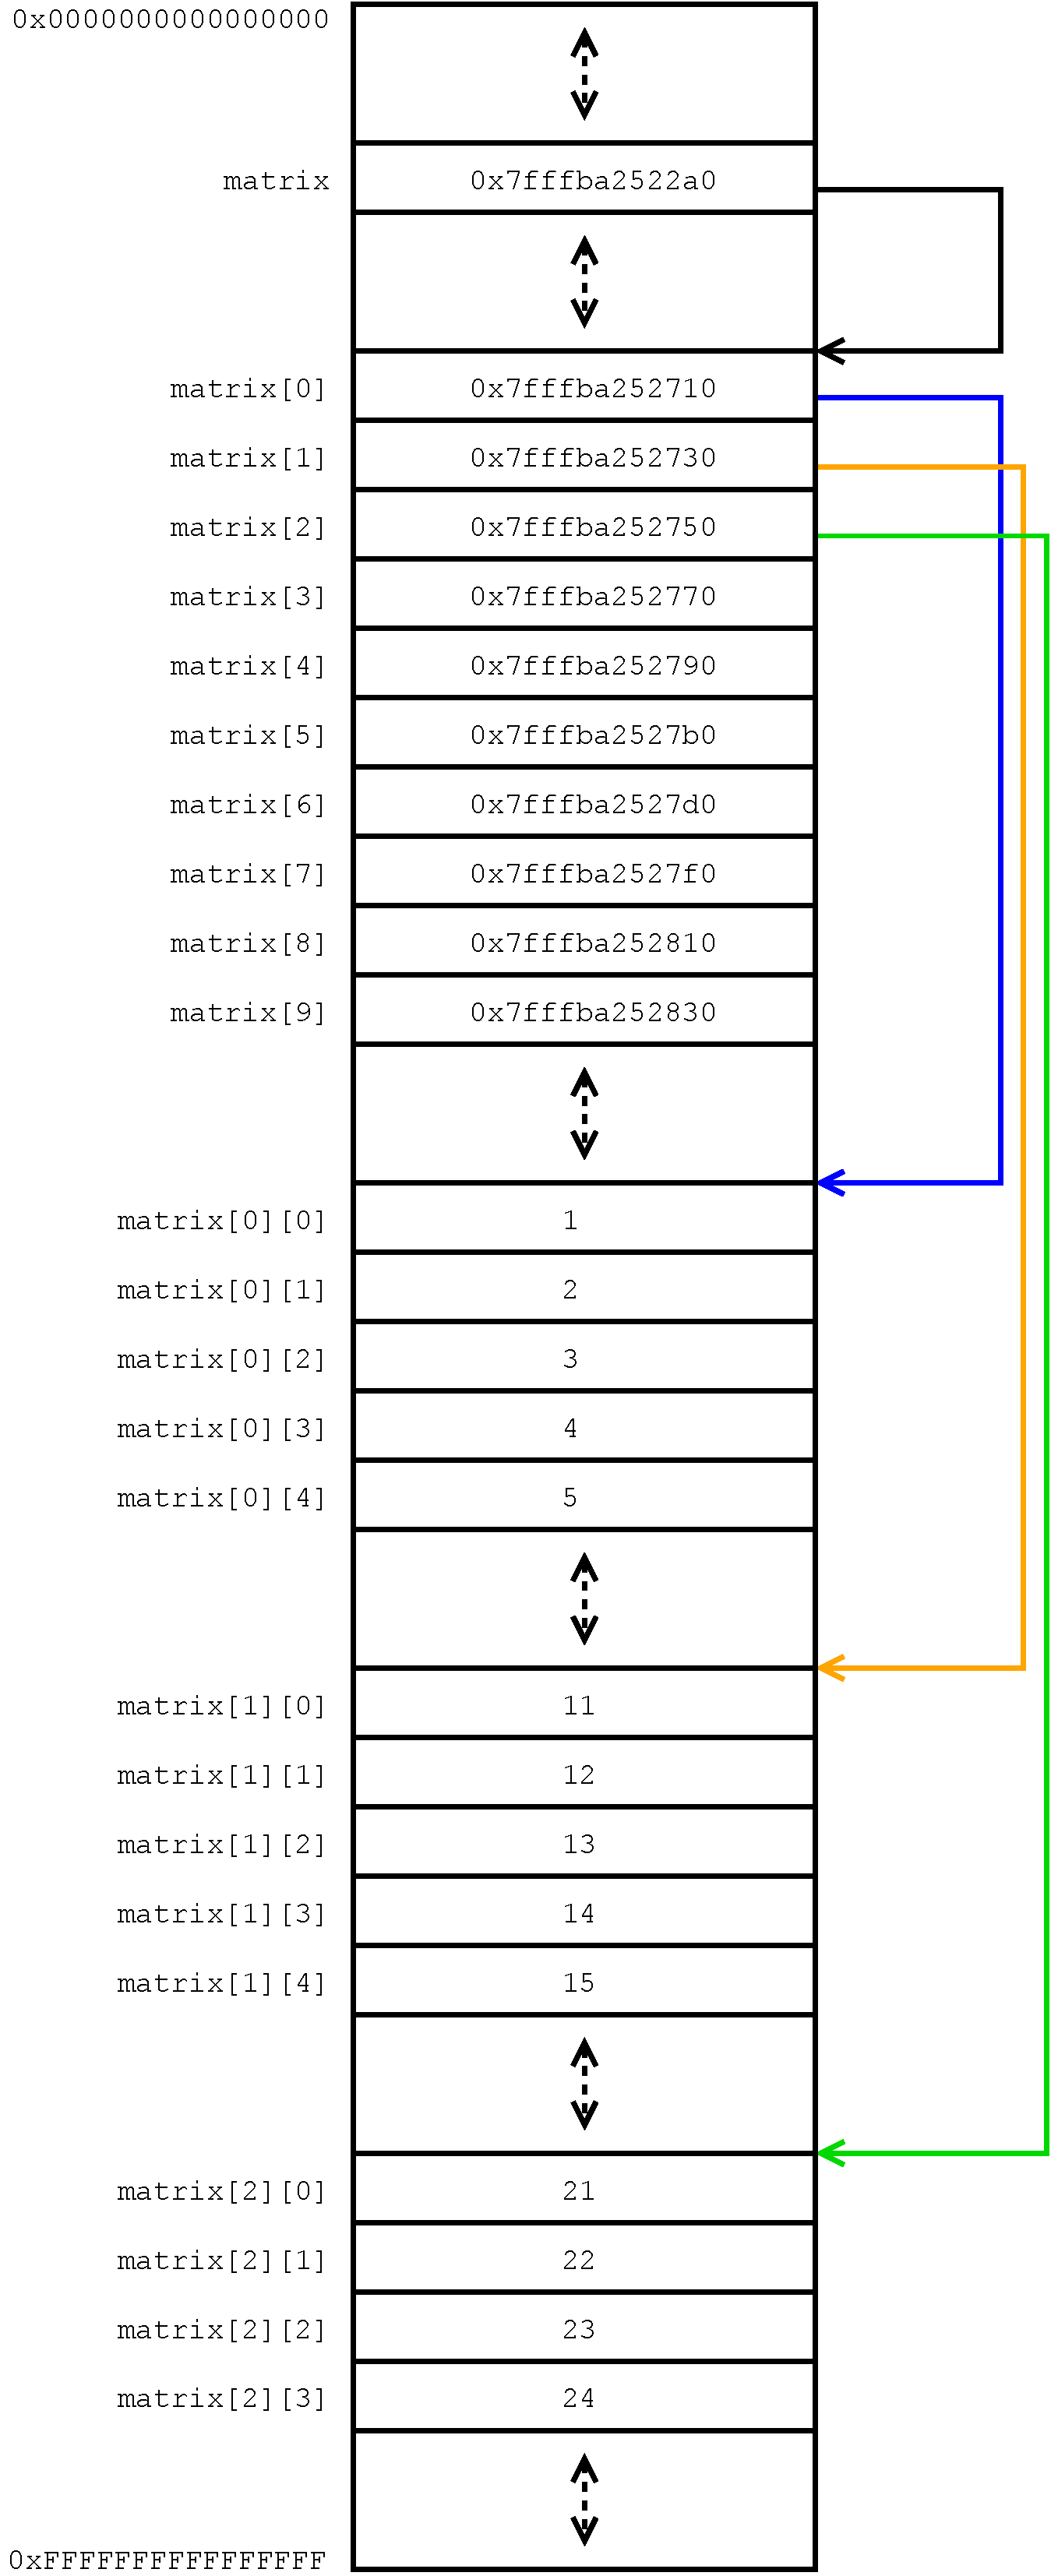
\includegraphics[height=225mm]{double_pointer_map}
    \caption{Mapa de memoria de un vector de vectores (doble puntero)}
    \label{img:double_pointer_map}
\end{figure}

In the figure I present the memory map, on the left there are the names those
locations have in the program, and in the rectangle I write their contents.
Arrows on the right side of the image represent the references of the pointers
to those memory addresses. Colors simply allow you to follow the different
arrows more easily. Well, if you look at where I put the tag \verb!matrix!,
you'd see it contains a memory address, this address references to a
\textbf{vector of pointers}, that is, \verb!rows! pointers together. Each one of
those pointers, to a contigous memory region in which the is an antire row
saved. I have only represented the first three rows, because otherwise the image
would be too big.

Now I am going to draw the figure on how would the map be in the case of a
double array, I don't include the code bcause it would be simply:
\lstinline[style=C]!int matrix[10][5]!.

\begin{figure}[H]
    % Lo centramos
    \center
    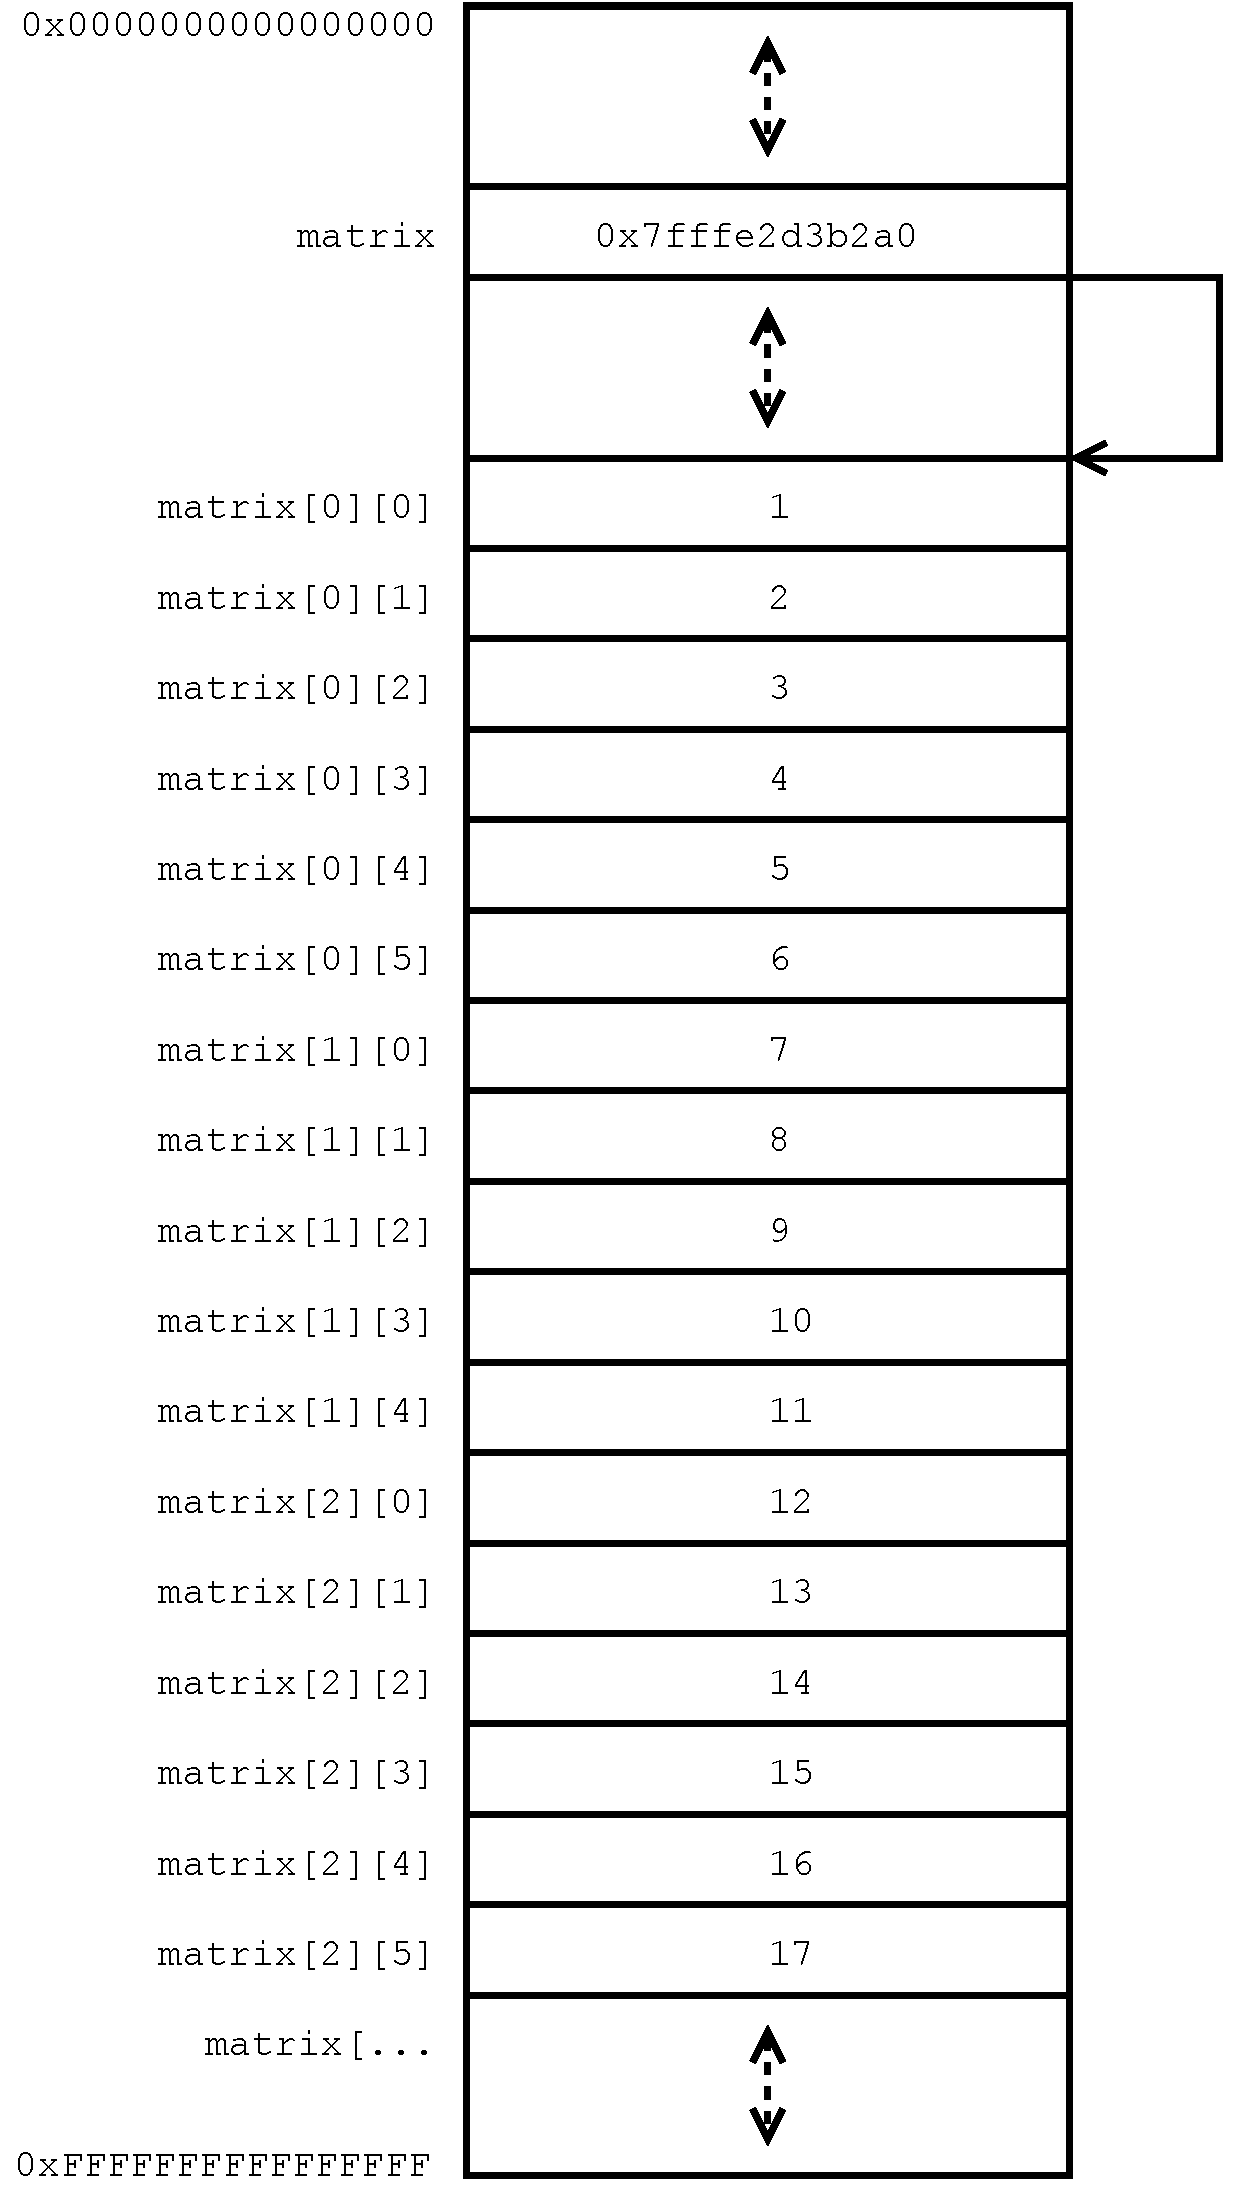
\includegraphics[width=.5\linewidth]{double_array_map}
    \caption{Memory map of a double array}
    \label{img:double_array_map}
\end{figure}

As you can see, even when the array have been declared with two dimensions,
there is not dereferenciation. That is: there is no moment in which you follow a
second pointer. How is this possible? If you look to the map, you'd see the
array is stored in a contigous memory region. This meand that C only needs to
adquiere the start address of the array and, later, add what the indexes
inside the square brackets tell you. It's here where a problem arises when we
try to pass a bidimensional array to a function. When the array reached the
function, C doesn't know if that pointer is a bidimensional array or a vector
of vectors, that is why, if you passed this array to a function that receives a
double pointer (\verb!int**!), when performing, for example \verb!matrix[1][2]!
what it would try to do is accessing it like it's a pointer, and would do:
\verb!*((*(matrix + 1))+2)!. That is, it would firstly add one to the base
address (remember pointer arithmetic) and then \textbf{it would interpret the
content as a pointer} to another vector and it would try to add 2 to that
address to dereference it. The problem is that \verb!*(matrix+1)!
\textbf{is not} a pointer, it is directly a number.

C can do this because, in the same that I explained you how the operator
\verb!sizeof! works, we can see the C knows the size of an array as long as this
does not decay to pointer, that is, you can know the size of an array in any
scope inner to the one it was declared in.

The logic conclusion of what we have just learnt is that maximun number of
dimensions of an array that any function can get is one, because it is the one
that behaves as a pointer without problems. The fact that an array, by being
declared in a unique order, is contiguous, makes arrays able to be accessed
always a one dimensional structures. For example, in the next code we declare and
fill up an array of two dimensions and, nevertheless, we can access it like if
it had just one dimension.

\noindent
\begin{minipage}[H]{\linewidth}
\mbox{}
\begin{lstlisting}[style=C,
caption={Using a bidimensional array like a one-dimension structure},
label={lst:bidimensionalArrayAsOneDimension}]
#include <stdio.h>
#include <stdlib.h>

int main(void)
{
    int rows = 10;
    int columns = 5;
    int matrix[10][5];

    printf("matrix = %p\n", matrix);

    for (int ii = 0; ii < rows; ++ii) {
        for (int jj = 0; jj < columns; ++jj) {
            matrix[ii][jj] = ii * columns + jj + 1;
        }
    }

    for (int ii = 0; ii < rows * columns; ++ii) {
        printf("%d\n", (*matrix)[ii]);
    }

}
\end{lstlisting}
\end{minipage}

As you can see, once we have reached the contiguous memory region
(\verb!(*matrix)!), we only have to iterate over it like if it were a one
dimension array.

\subsection{Section exercises}
\begin{exercises}[resume*]
\item Fill up this table with different numeric bases:
\begin{table}[H]
\begin{tabularx}{\linewidth}{|R|R|R|}
\hline
\multicolumn{1}{|Y|}{\textbf{Decimal}}& \multicolumn{1}{Y|}{\textbf{Binary}} & \multicolumn{1}{Y|}{\textbf{Hexadecimal}} \\\hline
73&  &  \\\hline
   &00100110& \\\hline
&&0x12F       \\\hline
128&&         \\\hline
\end{tabularx}
\end{table}
\item Return to the code of the 9\textsuperscript{th} exercise and reproduce
the content of the stack in all the code blocks of the program. Use as code the
solution I propose in the solution section.
\item Write a program that creates a pointer of three levels of type \verb!int!,
allocates memory for it correctly and fills it up with correlative values
\textbf{starting in one} and later on it prints it in an understandable way.
Finally, free it also in a way that the is no left unfreed memory at the end of
the program.
\item Using the last program as base, create two functions, one to create a
tridimensional matrix with dynamic memory given its three dimensions and another
one to free it.
\end{exercises}
\section{Type modifiers: const and sign}
\label{sec:typeModifications}
Up until now we have only used basic types, but you can add \textbf{modifiers}
to those types, which are qualities that create a slightly different type based on
the original one. The first and most important is the \lstinline[style=C]!const!
modifier. This allows us to indicate that the value of a variable is
\textbf{read only}, that is, once we give it value, and we must do so when
declaring it, we couldn't modify it. This is very useful to make sure we do not
introduce errors in the code when we use data that shouldn't be changed.

For example, imagine a program that uses the number $\pi$. Let's say to
calculate the area of a circle, we would need to write
\verb!surface = PI * r * r!, but imagine we make an error and write
\verb!surface = PI *= r * r!, this error would be difficult to catch because
the first time the surface would be correctly calculated, but \verb!PI! would
have a different value because we have unwillingly used the operator \verb!*=!,
and all the later calculations would be erroneous. If we declare \verb!PI! as
a constant, the compiler could notify us about those errors.

\noindent
\begin{minipage}[H]{\linewidth}
\mbox{}
\begin{lstlisting}[style=C,
caption={Uso de una constante numérica},
label={lst:constantUsage}]
#include <stdio.h>
#include <stdlib.h>

const double PI = 3.141592;

double surface_circle(double radius) {
    return PI * radius * radius;
}

double perimeter(double radius) {
    return 2 * PI * radius;
}

int main(void)
{
    double r = 3.5;
    printf("A circle with a radious of %.3f has a perimeter of %.2f and an area of %.2f\n", r, perimeter(r), surface_circle(r));
}
\end{lstlisting}
\end{minipage}

In line four you can see how we declare \verb!PI! as a constant of type
\verb!double!. You can see, also, we are declaring it as a global variables. If
you remember when I explained the scope and what global variables are, I told
you they would be useful once we had functions. Here you can see one of the most
common uses of them, when you define universal contants, as $\pi$, $e$ or the
gravitational constant $G$. But coming back to the constant, if you try to write
an instruction that modifies the constant, the compiler would throw an error
like this one:

\noindent
\begin{minipage}[H]{\linewidth}
\mbox{}
\begin{lstlisting}[style=terminalStyle]
\$  gcc -o main.exe main.c
main.c: In function 'main':
main.c:17:8: error: assignment of read-only variable 'PI'
   17 |     PI = 1.1;
      |        ^
\end{lstlisting}
\end{minipage}

But the \verb!const! modifier is applied in other place, it is used in the
declaration of arguments of functions to indicate that those cannot be modified.
Again, arguments of functions are copies of their values, so, knowing this,
it wouldn't make any sense to say we can't modify them, the core matter about
this is that the \verb"const" modifier is applied to pointers, indicating that
their content can't be modified, and this is where it is tremendously useful
when joined with functions. For example, let's go back to the function that
calculates the distance between two points using pointers, since we do not want
the structure to be modified by the function, we can do this:

\noindent
\begin{minipage}[H]{\linewidth}
\mbox{}
\begin{lstlisting}[style=C,
caption={Uso de punteros constantes como argumentos de función},
label={lst:constantArguments}]
#include <stdio.h>
#include <stdlib.h>
#include <math.h>

struct point_s {
    double x; double y;
};

double distance(const struct point_s* a, const struct point_s* b) {
    double res = 0.0;
    struct point_s origin = { .x = 0.0 , .y = 0.0 };
    if (NULL == a) {
        a = &origin;
    }
    if (NULL == b) {
        b = &origin;
    }
    double diff_x = a->x - b->x;
    double diff_y = a->y - b->y;
    res = sqrt(diff_x * diff_x + diff_y * diff_y);
    return res;
}

int main(void)
{
    struct point_s a = { .x = 3 , .y = 4 };
    double d = distance(&a, NULL);
    printf(" Distance : %f\n", d);

}
\end{lstlisting}
\end{minipage}

If you look at the program, the only difference is that in the declaration we
put \verb!const! before the data type. This avoids that we modify the content
of that pointer inside the function. If you try to perform for example:
\verb!a->x++;! the compiler will throw an error. This is very useful for the
programmer that uses the function if he hasn't written it, because that
declaration is a way to tell him that the function does not modify the data at
all. When we reach the point of writing our programs in different source files,
we will see this in more depth.

Also, the modifier \verb!const! adds the concept of \textbf{const correctness},
this concept means the programmer needs to respect the quality of constance of
variables and arguments. This means that you must define your functions
carefully, indicating everything you can as constant. For example, in the
case of the function that calculated the distance between two points, both
arguments must be constant. But there is more, the function \textbf{can return a
constant}. This is useful when you create structs that you do not want the user
to modify, but only with the functions you provide for that.

We will talk about this further later on, but I am going to set a basic example:
imagine a struct that saves data of a person. In this struct we would have
several pointers to \verb!char!: the name, the first surname and the second
surname (I wrote this example for Spanish names, which have two surnames). What
we will do is to create a function that receives three texts, will allocate the
necessary memory and we are going to create functions that replace those vectors
when the user of the functions needs to do so. Let's go:

\noindent
\begin{minipage}[H]{\linewidth}
\mbox{}
\begin{lstlisting}[style=C,
caption={Struct with const pointers -- Managing functions},
label={lst:structConstPointers}]
#include <stdio.h>
#include <stdlib.h>
#include <string.h>

struct person_s {
    char* name;
    char* last_name_1;
    char* last_name_2;
};

struct person_s person_create(const char* name,
                              const char* last_name_1,
                              const char* last_name_2) {
    struct person_s res;

    res.name        = malloc(strlen(name) + 1);
    res.last_name_1 = malloc(strlen(last_name_1) + 1);

    for (int ii = 0; ii < strlen(name) + 1; ++ii) {
        res.name[ii] = name[ii];
    }

    for (int ii = 0; ii < strlen(last_name_1) + 1; ++ii) {
        res.last_name_1[ii] = last_name_1[ii];
    }

    if (NULL != last_name_2) {
        res.last_name_2 = malloc(strlen(last_name_2) + 1);
        for (int ii = 0; ii < strlen(last_name_2) + 1; ++ii) {
            res.last_name_2[ii] = last_name_2[ii];
        }
    }
    else {
        res.last_name_2 = NULL;
    }
    return res;
}

void person_set_name(struct person_s* person, const char* name){
    free(person->name);
    person->name = malloc(strlen(name)+1);
    for(int ii = 0; ii < strlen(name) + 1; ++ii){
        person->name[ii] = name[ii];
    }

}

void destroy_person(struct person_s *person){
    free(person->name);
    free(person->last_name_1);
    free(person->last_name_2);
}
\end{lstlisting}
\end{minipage}

\noindent
\begin{minipage}[H]{\linewidth}
\mbox{}
\begin{lstlisting}[style=C,
caption={Struct with const pointers -- Functions to retrieve information},
label={lst:structConstGetters}]
const char* person_get_name(const struct person_s* person) {
    return person->name;
}

const char* person_get_last_name_1(const struct person_s* person) {
    return person->last_name_1;
}

const char* person_get_last_name_2(const struct person_s* person) {
    if (NULL == person->last_name_2) {
        return "";
    }
    else {
        return person->last_name_2;
    }
}

\end{lstlisting}
\end{minipage}

\noindent
\begin{minipage}[H]{\linewidth}
\mbox{}
\begin{lstlisting}[style=C,
caption={Struct with const pointers -- \texttt{main} function},
label={lst:structConstMain}]
int main(void)
{
    struct person_s myself = person_create("Francisco", "Rodríguez", "Melgar");

    printf("Esta persona es: %s %s %s\n", person_get_name(&myself),
            person_get_last_name_1(&myself),
            person_get_last_name_2(&myself));

    person_set_name(&myself, "José");

    printf("Esta persona es: %s %s %s\n", person_get_name(&myself),
           person_get_last_name_1(&myself),
           person_get_last_name_2(&myself));

    destroy_person(&myself);
}
\end{lstlisting}
\end{minipage}

In this code you can see how we ``hide'' the user how we manage these pointers.
To avoid him from chaging its content without using our functions, the functions
that return the pointers to be able to use them, for example to print them,
return constant pointers. If you tried to do, for example:
\lstinline[style=C]!person_get_name(&myself)[3] = 'a'! the compiler would throw
and error. This is a tool to avoid the user of the struct from forgetting to
free the memory when replacing a text by other.

If you're paying attention, you may have noticed that all of this is a little
bit useless when the use can simply write something like:
\verb!myself.name[0] = 'a'! and you'd be right. In later sections we would see
ways to avoid this. But, even with this problem, doing this is a good way to
save work to the user of the struct.

Another modifier I want to present to you is the sign, or better said, the
absence of sign. The keywork \lstinline[style=C]!unsigned! allows us to
declare variables and arguments of the same types of the basic types, but that
can only contain positive integers. If you do not see at first sight why this is
useful, this resides in that making a type unsigned you get a range doubled in
the possitive side. If a \verb"char" has a range of $[-127, 128]$, an unsigned
char has a range of $[0, 255]$. Also, this allows to add meaning to your
variables.

For example, a variable that stores the size of something, for example an array,
or a vector, shouldn't have a sign, because it can never be negative. A variable
that stores a month, shouldn't either, for instance. In the case of sizes of
vectors it is important to make the variable that stores their size unsigned,
because this allows us to get vectors and arrays of double the size. There are
not types without sign for floating point numbers (\verb!float! and
\verb"double"). Let's see an example on how to use the modifier \verb!unsigned!
to declare variables, arguments and return types.

\noindent
\begin{minipage}[H]{\linewidth}
\mbox{}
\begin{lstlisting}[style=C,
caption={Use of unsigned types},
label={lst:unsignedTypes}]
#include <stdio.h>

unsigned int factorial(unsigned int n) {
    unsigned int res = 1;
    for (unsigned int ii = 0; ii < n; ++ii) {
        res *= n - ii;
    }
    return res;
}

int main(void)
{
    unsigned int number = 10;
    printf("%d! =%d\n", number, factorial(number));
}
\end{lstlisting}
\end{minipage}

I know it looks a bit cumbersome to write unsigned each time, later on we will
see how to solve this.
\subsection{Exercises of the section}
The most appropiate exercise is for you to revise all the exercises we have done
and rewrite the code having into account the const quality and the sign.

\section{Communicating your program}
At last, we're reaching the part of the manual where you can communicate your
program with things outside it, up until now, all the data we have introduced in
the program are written as literals. This is very impractical, generally, a
program will read, either from the terminal or from a concrete file, the data
it is going to use. There are three sources of external information for a
program we're going to see in this manual (there are many more):
\begin{enumerate}
    \item Arguments from the command line.
    \item Input from the terminal.
    \item Files
\end{enumerate}

The first thing is something you do not know yet, but it's going to be very
useful. Up until now, \verb!main! function wasn't receiving any argument, but
how can it do so? If \verb!main! is the function that only acts as the entry
point for our program, who can call it with arguments? Basically these arguments
come from the command line we have executed our program with. To be able to
access them inside the program, we must declare the function \verb!main! in this
new way:

\noindent
\begin{minipage}[H]{\linewidth}
\mbox{}
\begin{lstlisting}[style=C,
caption={Declaration of a \texttt{main} function that receives arguments},
label={lst:mainArguments}]
int main(int argc, const char** argv) {
// ...
\end{lstlisting}
\end{minipage}

Of these two arguments of the function, the first one is the number of arguments
the program has
received, and the second is a vector of vectors of \verb!char! that is sent to
us as a two-level pointer. The arguments that a program receives come in text
format so, if they're numbers, you must use some functions to turn them into
those data types. Let's make a program that receives an undeterminated number
of arguments and prints them, each one in a new line.

\noindent
\begin{minipage}[H]{\linewidth}
\mbox{}
\begin{lstlisting}[style=C,
caption={Ussage of the arguments or a program},
label={lst:argumentProgram}]
#include <stdio.h>

int main(int argc, char const *argv[])
{
    for (int ii = 0; ii < argc; ++ii) {
        printf("%s\n", argv[ii]);
    }
}
\end{lstlisting}
\end{minipage}

Maybe you're wondering how can we pass those arguments to the program, after the
path of the executable, you write all the arguments separated by spaces, for
example:
\begin{lstlisting}[style=terminalStyle]
\$./main.exe argument1 argument2 argument3
\end{lstlisting}
If you compile the program and execute it with those arguments, it will print
this:

\begin{lstlisting}[style=terminalStyle]
./main.exe
argument1
argument2
argument3
\end{lstlisting}

And yes, as you can see, the first argument is the command you called the
program with, and this is important because, as you may deduct, this means
that your programs always receives at least one. This first argument changes
according to the order you executed your program with, for example, if instead
of with that path you'd execute it with an absolute path, you'd get the
following.

\begin{lstlisting}[style=terminalStyle]
\$ /home/usuario/test/project/main.exe arg1 arg2 arg3
/home/usuario/test/project/main.exe
arg1
arg2
arg3
\end{lstlisting}

As a last note, if the space is the character that separates the arguments, how
do we write arguments with spaces in them? Simply surround the argument between
straight quotes (like C strings). Let's see an example.
\begin{lstlisting}[style=terminalStyle]
\$ ./main.exe "This is a double quote: \"" \"\"\" "Sentence with spaces"
./main.exe
This is a double quote: "
"""
Sentence with spaces
\end{lstlisting}

If we need to read a number, we must use, as we said before, a function that
turns the text into a number. The basic function to do this is \verb!atoi!
(from ASCII to integer). For example, let's create a program that receives a
series of numbers and adds them up.

\noindent
\begin{minipage}[H]{\linewidth}
\mbox{}
\begin{lstlisting}[style=C,
caption={Program that adds its arguments},
label={lst:sumArgs}]
#include <stdio.h>
#include <stdlib.h>

int main(int argc, char const* argv[])
{

    int total = 0;

    for (int ii = 1; ii < argc; ++ii) {
        total += atoi(argv[ii]);
    }

    printf("The addition of the arguments is: %d\n", total);
}
\end{lstlisting}
\end{minipage}

Mind that we start adding from the second argument (position one in the vector)
because the first one is not a number. This leads me to warn you that
\verb!atoi! is a very basic function and that if you pass something to it that
is not a number, it will return nonsense values, many times zero. So be careful
about this. Anyway, in other sections we will see ways to manipulate text
strings that are more complex and would allow us to check it. It would be an
interesting exercise that you made a program that checks if a text string is a
number or not. Finally, there is also \verb!atof! that does the same, but for
floating point numbers.

Another option is to allow the user to write things into the program once
it has started. For example, we could write a program that is a 2.0 version of
our first \textit{Hello, World}. This version would firstly ask the name of the
user and then say hello to him personally. You can use the function \verb!scanf!
to do so. This function is the twin of \verb!printf! because it behaves in the
same way, you specify a format and pass the variable you need to it where it
will store the data. For example, let's make this \textit{Hello World 2.0}

\noindent
\begin{minipage}[H]{\linewidth}
\mbox{}
\begin{lstlisting}[style=C,
caption={\texttt{scanf} basic example},
label={lst:basicScanf}]
#include <stdio.h>
#include <stdlib.h>

#define NAME_LENGTH ((size_t)1024)

int main(int argc, char const* argv[])
{

    char name[NAME_LENGTH] = "";
    printf("Hello, what's your name?\n");
    scanf("%s", name);
    printf("Nice to meet you, %s.\n", name);
}
\end{lstlisting}
\end{minipage}

As you can see, it's easy, but you must be aware that if you read basic types
you must pass the pointers to the variable your want to store them in to
\texttt{scanf}. With this \verb!char! pointer it's less evident. Also, unless
you call other functions to change how the terminal behaves, \verb!scanf! will
only read up until the first whitespace character. That is, until the first
space. This means that if you want to read several words at the same time you
must call \verb!scanf! several times or call it with several format specifiers.
Let's see a bit more complicated example.

\noindent
\begin{minipage}[H]{\linewidth}
\mbox{}
\begin{lstlisting}[style=C,
caption={\texttt{scanf} advanced example},
label={lst:scanfExample}]
#include <stdio.h>
#include <stdlib.h>

#define NAME_LENGTH ((size_t)1024)

int main(int argc, char const* argv[])
{

    char name[NAME_LENGTH] = "";
    int age = 0;
    double height = 0.0;
    printf("Hello, I want to get to know you, tell me your name, age and how tall are you in meters.\n");
    scanf("%s %d %lf", name, &age, &height);
    printf("Nice to meet you, %s. So you're %d years old and are %f m tall.\n", name, age, height);
}
\end{lstlisting}
\end{minipage}

As we said, \verb!scanf! stops reading in the first space, so your can write
each data and hit enter or write the three answers separated by spaces and hit
enter just once. Also, note that, as you want to read a \verb!double! we must
use the specifier \verb!%lf!, the
compiler would warn us this is not right if we used \verb!%f!. This function
\textbf{blocks} the program until is receives \textbf{all} the arguments we're
asking for with the specifiers. Also, what is written in the terminal and does
not get used (is read with \verb!scanf!) stays there pending to be used. That
is, if instead of writing our example with just one call to \verb!scanf! we
wrote three calls, each one with one specifier and variable, the effect would be
the same. You could still write the three things separated by spaces and hit
enter. In the same way that \verb!atoi!, if the specifiers expects a number and
the input is not a number, the function will fail throwing values with little to
no sense.

Finally, the files. Programs can delete, create, write and read from files.
To do this, there are several ways, some more simple than others, because some
are more standard and other depend on the operating system. In opposition to the
other methods, files have a more complex life cycle. Life cycle in this context
refers to the description of when something starts to exist, exists and ceases
to do so. For example, the life cycle of a dynamically reserved memory block is
from the moment of their allocation to the moment it's freed, the one of an
array goes from the moment you go into the block of code it's declared to the
moment the program stops executing in that block.

Files are a concept that, again, the operating system manages, therefore we have
to use functions to open, write, read from them and, finally, close them. If you
have been paying attention, you may have seen the parallelism between this and
memory allocation. The function to open a file is \lstinline[style=C]!fopen!,
let's see its declaration.

\noindent
\begin{minipage}[H]{\linewidth}
\mbox{}
\begin{lstlisting}[style=C,
caption={\texttt{fopen} function declaration},
label={lst:callocSignature}]
FILE *fopen(const char *pathname, const char *mode);
\end{lstlisting}
\end{minipage}

It returns a pointer to a type called \verb!FILE!, this type is \textbf{opaque},
this a word that it is used in computer science to say that you can't know what
is inside, that is, it is the system who manages it and you only interact with
it calling the functions it provides you. The arguments this functions receives
are two \texttt{char} pointers. The first one is the path to the file. This path
takes as origin \textbf{the working directory} of the terminal where we
executed the program. That is, if you pass to the function the path
\verb!./file.txt!, it will look for it (or create it, depending on how the
function was called), in your working directory, no in the one the program is
in, unless they're the same.

The second argument is interesting, it is, as its name says, the mode in which
we're opening the mode. In this argument you tend to write a literal that
contains a series of letters, these letters are the attributes of the way you're
going to open the file. Let's see which options we have.
\begin{enumerate}
    \item \verb!r!: Open the file just to read it, the reader head (more on this
    later) is at the
    start of the file. If the file does not exist, an error occurs and the
    function returns \verb!NULL!.
    \item \verb!r+!: Same as before, but it allows to write too.
    \item \verb!w!: \textbf{Empties} the file or creates it if it doesn't exist.
    The reading head is at the start, logically.
    \item \verb!w+!: Like the last one, but allows to read too.
    \item \verb!a!: Open the file to write in it, but \textbf{it does not empty
    it}. It creates it if it doesn't exist, the head start at the end of the
    file, to \textbf{append} data to it.
    \item \verb!a+!: The file is created if it does not exist, data will be
    written to the end of the file. It also allows reading.
\end{enumerate}

In the description of the options I talk about something called the reading or
writing head, also called read/write pointer. It is not a C pointer or anything
like that. It is a concept inherent to files. The read/write head is an abstraction
of a physical device that is in a point of the file and writes or reads to it.
Files are just a stream of bytes, and this head would write or read from the
position it is in, and advance as many bytes as it read or wrote. The methaphor
that was used was a video tape. If you put a tape in a video player, the head
would start at the begining of the tape, if you watched let's say ten minutes
of it, you could pause it, go do something and come back, it will be where you
left it. You could rewind it, fast forward it, etc. Also, playing the video
makes the head move forwards, that is: reading makes you rewind if you want
to read the same thing again.
All this being said, the read/write header is unique \textbf{per
file and process}, this means that two programs can be reading or writing from
the same file at the same moment but in different positions.
When you reach the end of the file you can't
read more (logically) but if you're writing, the file would grow seamlessly.

Now you already know how to open a file, let's see how to write or read to and
from it. The functions that are used to do this are these two: \verb!fwrite!
and \verb!fread!

\noindent
\begin{minipage}[H]{\linewidth}
\mbox{}
\begin{lstlisting}[style=C,
caption={\texttt{fread} function signature},
label={lst:freadSignature}]
size_t fread(void *ptr, size_t size, size_t nmemb, FILE *stream);
\end{lstlisting}
\end{minipage}

\noindent
\begin{minipage}[H]{\linewidth}
\mbox{}
\begin{lstlisting}[style=C,
caption={\texttt{fwrite} function signature},
label={lst:fwriteSignature}]
size_t fwrite(const void *pt, size_t size, size_t nmemb, FILE *stream);
\end{lstlisting}
\end{minipage}

The two functions behave more or less the same, they receive a pointer, a size,
another number a finally the pointer to the struct that symbolizes the file.
The first pointer is the input to write and the output to read. It is where we
will put our data, or the memory so the function can write the content
of the file in it. It is a \verb!char! pointer, which is the kind of pointer
used when you want to manage a generic stream of bytes. Both functions are
written with the idea of managing a number of items of a certain size in
bytes, that's why we have \verb!size! and \verb!nmemb!. The first one is the
size of the items we're writing or reading and the second the number
of said items we're reading or writing. The function returns the number of
\textbf{items} written or read, not the number of bytes, mind this when
using the functions.
More on this in the examples later on.

Finally, after doing what you want with the files you have opened, you must
close it. Closing the files makes all the changes you have done to it to be
written with the underlying storage device. This is important, if you forget to
close a file you may see the changes you've done in your program are not
in the real file. The function to close files is called \verb!fclose! and its
signature is like this:

\noindent
\begin{minipage}[H]{\linewidth}
\mbox{}
\begin{lstlisting}[style=C,
caption={\texttt{fclose} signature},
label={lst:fcloseSignature}]
int fclose(FILE *stream);
\end{lstlisting}
\end{minipage}
As you can see, it only receives the pointer to the file we can to close.

Now we have shown the functions that are needed, let's an example on how to use
files. A very usual program is one that copies a files from one directory to
another, like the command \verb!cp!, which is the one used in Linux to do so.
Let's make a program that receives two arguments, the first one would be the
file we want to copy and the second the folder we want to copy it to. The Linux
command allows the use to specify a folder as destiny, but to make things
simpler we will make this program to ask for a full path (name of the destiny
file) included.

\noindent
\begin{minipage}[H]{\linewidth}
\mbox{}
\begin{lstlisting}[style=C,
caption={Example of basic file management},
label={lst:fileBasic}]
#include <stdio.h>
#include <stdlib.h>

int main(int argc, char const* argv[])
{

    FILE *origin_file  = NULL;
    FILE *destiny_file = NULL;
    char byte          = 0;

    if (argc < 3) {
        printf("Use: main.exe <origin> <destiny>\n");
        return EXIT_FAILURE;
    }

    origin_file = fopen(argv[1], "r");

    if (NULL == origin_file) {
        printf("ERROR: The origin file doesn't exist.\n");
        return EXIT_FAILURE;
    }

    destiny_file = fopen(argv[2], "w");

    if (NULL == destiny_file) {
        printf("ERROR: The destiny file doesn't exist.\n");
        fclose(origin_file);
        return EXIT_FAILURE;
    }

    while (0 != fread(&byte, sizeof(char), 1, origin_file)) {
        fwrite(&byte, sizeof(char), 1, destiny_file);
    }

    fclose(origin_file);
    fclose(destiny_file);
    return EXIT_SUCCESS;
}

\end{lstlisting}
\end{minipage}

As you can see, we have declared two variables of the pointer type to
\verb!FILE!, we initialize them to \verb"NULL" and start the program. When you
receive arguments it is adviceable to parse them first, because if they are not
correct, there is no purpose in continuing with the program. After that, we try
to open the origin file, note that we open it just to read it and without
emptying it, logically. If that call fails, the value it return would be
\verb!NULL! and we check this is not the case before continuing. We do the
same with the destiny
file, but this one is opened with the option \verb!r! that will empty the file
if it exists and create it if it does not.
Notice that, in case of error, we need to close the first file we
opened before exiting the program (returning from function \verb!main! ends the
program). Finally, we use a loop to read byte by byte the origin file and write
it in the destiny. As you can see, the loop condition is that it will keep
looping as long as the reading function returns anything that is not zero.
This is like so because both \verb!fwrite! and \verb!fread! return the number of
items they have written or read. In this case, when \verb!fread! returns zero it
is there is no more to read.

I am going to take some time explaining the return value of the functions, as
we said before, we pass to both \verb!fread! and \verb!fwrite! a size and a
number of items we want to read or write. This would allow us for example to
write or read a certain number of structs whose size we could know with
\verb!sizeof!. The return value is the number os \textbf{items} read, not the
number or bytes. When writing a stream of bytes directly, simply indicate that
the size is one and \verb!nmemb! is the numbers of bytes.

You may be thinking that writing a program like this that reads one byte at a
time is a bit inefficient, and you're right. Each call to a function that
manages things that are handled by the operating system is relatively costly,
so it is intelligent to minimize them. In this case, we could read all the
first file in memory and then close it and write it in the second, in just one
order. The problem with this is that if you tried to cpy a 12~GB file it's
probable that you fill all the memory in the computer, in which case it simply
hangs or closes the program. To avoid both extremes, what is done often is to
read a block of a sensible size (for example 100~MB) and write it, and repeat
until the process is done.

\noindent
\begin{minipage}[H]{\linewidth}
\mbox{}
\begin{lstlisting}[style=C,
caption={Example of file copying with a buffer},
label={lst:readWithBuffer}]
#include <stdio.h>
#include <stdlib.h>

int main(int argc, char const* argv[])
{

    const size_t BLOCK_SIZE   = (size_t)(1024 * 1024);
    FILE*        origin_file  = NULL;
    FILE*        destiny_file = NULL;
    char*        buffer       = malloc(BLOCK_SIZE);
    size_t       bytes_read   = 0;

    if (argc < 3) {
        printf("Use: main.exe <origin> <destiny>\n");
        return EXIT_FAILURE;
    }

    origin_file = fopen(argv[1], "r");

    if (NULL == origin_file) {
        printf("ERROR: The origin file does not exist.\n");
        return EXIT_FAILURE;
    }

    destiny_file = fopen(argv[2], "w");

    if (NULL == destiny_file) {
        printf("ERROR: The destiny file does not exist.\n");
        fclose(origin_file);
        return EXIT_FAILURE;
    }

    while (0 != (bytes_read =
                     fread(buffer, sizeof(char), BLOCK_SIZE, origin_file))) {
        fwrite(buffer, sizeof(char), bytes_read, destiny_file);
    }

    fclose(origin_file);
    fclose(destiny_file);
    free(buffer);
    return EXIT_SUCCESS;
}
\end{lstlisting}
\end{minipage}

The only change is that instead of a single \verb!char! we declare a vector of
them with the size defined in a const variable and, later on, in the copy loop,
instead of copying always one byte, we try to read the block size and, when
writing it, we use the value returned from the read operation. I want to take a
moment in this line because it's a bit different from what we have seen up until
now. An assignment is an expression with a value. This is what allows us to do
things like: \verb!a = b = c!. Thanks to this property, you can compare the
result of an assignment to another value. In this case we could save writing the
comparison because putting a number in an if is the same that checking it is not
zero.

This is a basic use of reading and writing, but anochet thing that is done often
is \textbf{move the read/write pointer} without reading or writing. For example,
imagine that we want to print a file in reverse order. We are in the same
predicament as before, we could read all the file and then invert it, but it is
a problem again if the file is too big. We could do the same we did before, read
the file piece by piece, invert the pieces and then put them all together, also
in a reverse order. This is complicated, thanks to the fact we can move the
read/write pointer, we can read directly the blocks in reverse order.

\noindent
\begin{minipage}[H]{\linewidth}
\mbox{}
\begin{lstlisting}[style=C,
caption={Example of use of functions to move the read/write pointer},
label={lst:fseek}]
#include <stdio.h>
#include <stdlib.h>
#include <string.h>

#define BLOCK_SIZE ((long) 100)

void invert_bytes(char* stream, int length)
{
    for (int ii = 0; ii < length / 2; ++ii) {
        char temp = stream[ii];
        stream[ii] = stream[length - 1 - ii];
        stream[length - 1 - ii] = temp;
    }
}
int main(int argc, char** argv)
{
    long  current_pos = 0;
    FILE* file = NULL;
    if (argc != 2) {
        printf("Uso del comando: main.exe <archivo>\n");
        return EXIT_FAILURE;
    }
    file = fopen(argv[1], "r");

    if (NULL == file) {
        return EXIT_FAILURE;
    }

    fseek(file, 0, SEEK_END);
    current_pos = ftell(file);
    while (current_pos != 0) {
        char block[BLOCK_SIZE + 1] = {};
        long next_pos = 0;
        long block_size = 0;
        if (current_pos - BLOCK_SIZE < 0) {
            next_pos = 0;
            block_size = current_pos;
        }
        else {
            next_pos = current_pos - BLOCK_SIZE;
            block_size = BLOCK_SIZE;
        }
        fseek(file, next_pos, SEEK_SET);
        fread(block, 1, block_size, file);
        fseek(file, -block_size, SEEK_CUR);
        invert_bytes(block, block_size);
        printf("%s", block);
        current_pos = ftell(file);
    }
    fclose(file);
    printf("\n");
}
\end{lstlisting}
\end{minipage}

The program is a bit complicated, but, as always, we will explain it little
by little. The first thing we do is to define a function that can reverse the
bytes of a vector. It is not the main matter in this example, but remember the
algorithm because it is a classic. What we want to do starts right after, it is
a bit complex, but I am interested in you seeing what the functions that move
the head do. Up until line 27 the only thing we do is something you're already
used to see: we process the arguments and open the file, checking everything has
gone well. After that we use the function \verb!fseek! that allows us to
\textbf{move the read/write pointer}, concretely, we move it to the end of the
file. Let's see how it work.

This function allows us to move the head to a point in the file with an offset.
There are three points you can use as reference for the offset.
\begin{enumerate}
\item \verb!SEEK_SET!: The start of the file.
\verb!fseek(100, SEEK_SET);! would set the head to be in the
100\textsuperscript{th} byte of the file. When using this point, you cannot use
negative offsets, logically.
\item \verb!SEEK_CUR!: It is the current position, you can use negative of
positive displacements For example: \verb!fseek(100, SEEK_CUR);! could be used
in a loop to read the bytes 100\textsuperscript{th},
the 200\textsuperscript{th}, the 300\textsuperscript{th}...
\item \verb!SEEK_END!: It is the end of the file, for example if you wanted to
go to the third byte from the end you'd perform: \verb!fseek(-3, SEEK_END);!
\end{enumerate}

In line 29 what we do is going directly to the end of the file. After that,
we use another function called \verb!ftell!. This functions give us the current
position in the file as a number. That is how we know where we are. After that
we check if there is a whole block of data left. If we can, we use that block
size, if not, we use what we can. After that, we displace the head to the
position we have calculated, and read the amount of bytes we calculated. We read
and \textbf{displace the pointer back again} as many bytes as we read. After
that we call the function that inverts the bytes we have read. After that,
we update the variable that tell us where we are. Once we arrive to the first
position of the file, we know we have finished. You must be careful,
\verb!fseek! only works when it is possible to move the pointer to the place you
tell it to. When it is not possible, it doesn't move the pointer and gives an
error (returns -1). Finally, we close the file and print a new line so the
prompt shows in the next line.

We haven't used it in the example, but you can \textbf{delete} files. To do so
we use the function \verb!remove!, whose signature is:

\noindent
\begin{minipage}[H]{\linewidth}
\mbox{}
\begin{lstlisting}[style=C,
caption={\texttt{remove} function signature},
label={lst:signatureRemove}]
int remove(const char *pathname);
\end{lstlisting}
\end{minipage}

As you can see, it simply receives a path. Let's see an example of a simple
program that makes use of it: one that receives as an argument a path and
deletes it.

\noindent
\begin{minipage}[H]{\linewidth}
\mbox{}
\begin{lstlisting}[style=C,
caption={Example of a program that uses \texttt{remove}},
label={lst:exampleRemove}]
#include <stdio.h>
#include <stdlib.h>

int main(int argc, char const *argv[]) {
    if (argc != 2) {
        printf("Usage: ./main <path to the file>");
    }

    int error = remove(argv[1]);

    if (error == 0) {
        return EXIT_SUCCESS;
    } else {
        return EXIT_FAILURE;
    }
}
\end{lstlisting}
\end{minipage}

The program is very simple, I call remove with the first
argument (after the name of the program) and check is it has gone well.

\subsection{Exercises of the section}
\begin{exercises}[resume*]
\item Write a program that receives a set of number as arguments and prints
their decomposition in prime factors, for example, if the arguments were:
10, 8, 55 and 103, the result would be:

\noindent
\begin{minipage}[H]{\linewidth}
\mbox{}
\begin{verbatim}
Factors of
10: 2, 5
8: 2, 2, 2
55: 11, 5
103: 103
\end{verbatim}
\end{minipage}

It is recommended to make error control, checking the arguments are numbers
before using them, etc. Also, the order of the factors is not important.
\item Write a program that reads \textbf{from terminal} a series of words and
that only stops reading when you introduce ``!!'' as a word. After that, it
must print said words in a random order. The function \verb!rand! returns a
random number between zero and the biggest possitve integer, you need it to
generate random numbers. If you want the random numbers to be different from
one execution to the other, simply put this line: \verb!srand(time(NULL));! at
the begining of your program. If you decide to do this too, you need to add
the line \verb!#include<time.h>! just after the \verb!#include<stdio.h>! line.

\item Make a function that reads two files and \textbf{swaps} their content,
write said program in such a way that there is no need to store any of the files
in memory completely. To do this you may follow these steps.
\begin{enumerate}
    \item Copy the contents of the first file to an auxiliary file in
    \verb!/tmp/!.
    \item Close the file you have copied.
    \item Open it again with a mode that deletes the contents.
    \item Copy the contents of the second file to the first.
    \item Close the second file.
    \item Open it again with a mode that deletes its content.
    \item Copy the content of the auxiliary file to the first file.
    \item Delete the auxiliary file from \verb!/tmp/!.
\end{enumerate}

\item Write a function that receives a word as an argument and indicates
in which position (in bytes) a word is in a file. Return just the position of
the first ocurrence, if the word does not exists, return a negative number.
Write a program that, with that function, receives a path and a word as
arguments and prints the result of searching for the word in the file.
\end{exercises}

\section{How to write readable and clear programs}
All programming languages have a different degree of \textbf{readability}. This
is the easily a programmer would be to read the code written by another one, and
understand what it is doing without a high level of effort. The language is not
the only thing that affects the readability, the way one writes the code affects
it at least as much, if not even more. Some advices to write more readable code
are:
\begin{enumerate}
\item Use significative variable names, that is, instead of \verb!a!, call
variables things like \verb!length!, \verb!days!, or something that had anything
to do with their meaning, with what they are.
\item Use function names that explain what the function is doing, in the same
way, use names for the arguments that tell what they are, also.
\item Write the code indenting each new code block. More on this later.
\end{enumerate}

Also, in C there are two tools of vital importance to increase the readability
of code and that I am going to present to you now. One is the keyword
\lstinline[style=C]!typedef!. This keyword allows us to \textbf{give an alias
to a datatype}. That is, it allows to give other names to datatypes. One of the
most practical uses to this is that it allows us to refer with a single word to
refer to a struct, so we save the fact of writing \verb!struct mystruct_s!,
you can't avoid to tell me it's a relief after writing so many programs full of
the word \verb!struct!. Let's an example of this.

\noindent
\begin{minipage}[H]{\linewidth}
\mbox{}
\begin{lstlisting}[style=C,
caption={Definition of a type from a struct},
label={lst:structTypeDefinition}]
#include <stdio.h>

struct point_s {
    double x;
    double y;

};

typedef struct point_s point_t;

int main(void)
{
    point_t p = {.x = 3.3, .y = 1.1};
    struct point_s q = { 1,3 };
}
\end{lstlisting}
\end{minipage}

This would be the most explicit way to do this. There is another alternative
that we will see later on. From lines 1 to 4 there is nothing new, we simply
declare the struct, it is line 6 that is the key, as you can see, we use the
word \verb!typedef! to define the type \verb!struct point_s! is going to be
called also \verb!point_t!. Notice that, as you can see in line 14, we can keep
using the old name of the types. All this being said, unless you want to
symbolize something different to express a different meaning, it is better to
use always the same name for the types. There is a more abbreviated way to do
this, as a matter of fact, two, you can combine the sentence \verb!typedef! with
the struct creation in the same line. Doing this, you can choose to set a name
for the struct or not, because its ``real'' name would be the one you define
with \verb!typedef!. Let's see it:

\noindent
\begin{minipage}[H]{\linewidth}
\mbox{}
\begin{lstlisting}[style=C,
caption={Different combinations of \texttt{struct} with \texttt{typedef}},
label={lst:structTypeCombo}]
#include <stdio.h>

typedef struct point_s {
    double x;
    double y;

} point_t;

typedef struct {
    point_t center;
    double radius;
} circle_t;

int main(void)
{
    struct point_s p = { 1.1, 2.3 };
    point_t        q = { 1.2, 3.4 };
    circle_t  origin = { .center = {.x = 0, .y = 0}, .radius = 1 };
}
\end{lstlisting}
\end{minipage}

The two declarations of these two structs are equivalent in the fact that they
add a simple name to the structs, but with a nuance: the point struct keeps its
struct name, so it could still be used to declare variables of this type as it
is shown. The circle struct hasn't got an struct name, we have only used it
to define a type. This is simpler but it presents a problem, when you do this
and the compiler needs to tell you
there's been an error, they would be different depending on the technique we
use. With the struct \verb!circle_t!, if we declare one function that receives
an argument of this type and cell it with a different type, creating an error,
the message would be:
\begin{lstlisting}[style=terminalStyle]
main.c:14:18: note: expected 'circle_t' {aka 'struct <anonymous>'} but argument is of type 'int'
   14 | int foo(circle_t c){
\end{lstlisting}

As you can see, it sayd to you the name the type had, and then it tries to
explian to you what it was originally, the problem is that, since we have
defined the struct without a proper name, it has nothing to tell us, is an
anonymous struct. And you may be wondering how can that be possible, well it is
because in C you can declare structs without name like a variable to use them
and throw them away. I am going to show it to you, but it is something I haven't
seen in proffesional code so, like \verb!goto!, keep in mind it exists, but
it would be better if you do not use it.

\noindent
\begin{minipage}[H]{\linewidth}
\mbox{}
\begin{lstlisting}[style=C,
caption={Anonymous struct},
label={lst:anonymousStruct}]
#include <stdio.h>


int main(void)
{
    struct { double x; double y; } temporal_point = { .x = 1, .y = 2 };
    printf("This is a temporal point which is in [%1.2f, %1.2f]\n", temporal_point.x, temporal_point.y);
}
\end{lstlisting}
\end{minipage}

This is why we are able to define structs that have no name and and use this
anonymous struct to define a type. My advice is that you always put a name
to the struct to avoid the compiler to throw confusing errors. Compare this
error of the compiler with the other error for the struct point that has a
struct name regardless of \verb"typedef".

\begin{lstlisting}[style=terminalStyle]
main.c:13:18: note: expected 'point_t' {aka 'struct point_s'} but argument is of type 'int'
   13 | void foo(point_t p){
      |          ~~~~~~~~^
\end{lstlisting}

Finishing this with this topic: if you look closely, everytime I have put name
to a struct I have ended it with \verb!_s!, and each time I have written a
\verb!typedef!, I have ended it with \verb!_t!. This is a convention, that is,
it is something programmer do because of tradition, but it is not mandatory,
not the compiler would throw an error or warning. Es suffix \verb!_s! is less
important, but I strongly encourage you to end all the types you define with
\verb"typedef" with \verb!_t!, firstly: because it is very common, almost
everybody does it and, secondly: because editors understand that any
identificator (name, nasically), ends with a \verb!_t! is a type, and they use
it to give hints about what each thing is, for example, editor will colorize
that word in the color that editor colorizes types automatically if it ends with
\verb!_t!.

Aside from this very practical use for us, there is another, it allows us to
rename basic types, for example, we can rename the unsigned \verb!char! as
\verb!byte_t!. In that way if we use our program to manage lists of bytes we can
use this type and reader of our code will know what we're talking about.

\noindent
\begin{minipage}[H]{\linewidth}
\mbox{}
\begin{lstlisting}[style=C,
caption={Redefining basic types},
label={lst:typedefBasicType}]
#include <stdio.h>

typedef unsigned char byte_t;

void print_byte(byte_t b) {
    byte_t current_byte = 128;
    for (int ii = 0; ii < 8; ++ii) {
        printf("%d", (b & current_byte) != 0);
        current_byte /= 2;
    }
    printf("\n");
}

int main(void)
{
    print_byte(110);
}
\end{lstlisting}
\end{minipage}

Perhaps you do not understand all the code, the line 8, concretely, but simply
look at how using a concrete type makes everything more readable. Also, it
saves us to write unsigned several times. In the same way we did with the sign,
we can define types with the const modifier, for example:
\verb!typedef const char letter_t!.

\noindent
\begin{minipage}[H]{\linewidth}
\mbox{}
\begin{lstlisting}[style=C,
caption={Example of definition of a type with const modifier},
label={lst:typedefConstType}]
#include <stdio.h>

typedef const char letter_t;

letter_t dictionary[] = { 'a', 'b', 'c', 'd', 'e', 'f', 'g', 'h', 'i', 'j', 'k', 'l', 'm', 'n', 'o', 'p', 'q', 'r', 's', 't', 'u', 'v', 'w', 'x', 'y', 'z' };

int pos_of_letter(letter_t l){
    for(unsigned int ii = 0; ii < sizeof(dictionary); ++ii){
        if(l == dictionary[ii]){
            return ii + 1;
        }
    }
    return -1;
}

int main(void)
{
    letter_t l = 'f';
    printf("%c is letter number %d in the alphabet.\n", l, pos_of_letter(l));
}
\end{lstlisting}
\end{minipage}

Even when this is posible, it is better to leave the const modifier as explicit,
that is, define types for what u need, but write the modifier \verb!const! when
it is needed, instead of hiding it behind a typedef. It is a common practice
to define unsigned types, but it is recommended that, unless the meaning of the
type implies it can't be negative (for example a length), putting some prefix in
the name of the type. For example, you may see, if you read some code, types
like \verb!uint32_t! which is a 32-bit integer (4 bytes) without sign.

And for final trick, with \verb!typedef! this final trick is that, like arrays
of different positions are in a way different types, you can define a type from
an array. What is thif useful for? Sometimes a set of things of a certain size
is a concept itself. Eight bits are a byte, seven days is a week and a hand has
five fingers. Syntax for this is a bit different from what you may think at
first instance.

\noindent
\begin{minipage}[H]{\linewidth}
\mbox{}
\begin{lstlisting}[style=C,
caption={Definición de un tipo personalizado a partir de un array},
label={lst:typedefArrayType}]
#include <stdio.h>

typedef unsigned char pixel_t[3];

int main(void)
{
    pixel_t pixel = { 125,33,129 };
    printf("This pixel has these values: Red = %hu, Green = %hu, Blue = %hu\n", pixel[0], pixel[1], pixel[2]);
}
\end{lstlisting}
\end{minipage}

As you can see, \verb![3]! is on the right of the name of the new type, instead
of on the left, which would be the untuitive. Simply remember if you want to do
this. Anyway, in the same way that with contance, a type that is an array is
something that is better to leave explicit.

The other tool to add meaning to our programs, semantics, is the \verb!enum!, or
enumerated type. This is a type in C that allows us to assign correlative
numbers to a set of names, the classic examples (so classic they are almost
hackneyed) are the following: days of the week, months in the year, colors of
the rainbow... The utility of this is that we can codify easily sets of names
like those to names and use them to iterate a loop, index arrays, etc. Let's the
example of the days of the week.

\noindent
\begin{minipage}[H]{\linewidth}
\mbox{}
\begin{lstlisting}[style=C,
caption={Basic example of enumerated type},
label={lst:BasicEnum}]
#include <stdio.h>

enum week_days {
    MONDAY,
    TUESDAY,
    WEDNESDAY,
    THURSDAY,
    FRIDAY,
    SATURDAY,
    SUNDAY
};

int main(void)
{
    printf("Todays it is: %d\n", SATURDAY);
}
\end{lstlisting}
\end{minipage}

If you compile and execute this you will see that it prints: ``Today it is: 5''.
This is because when we write an \verb!enum! like that, the first element gets
the value zero, the next one, and so on... in this case from zero to six. And
the enumerated types can be more useful if you couple them with arrays of types
that help us to add meaning.

\noindent
\begin{minipage}[H]{\linewidth}
\mbox{}
\begin{lstlisting}[style=C,
caption={Enum used alongside name array},
label={lst:EnumWithNames}]
#include <stdio.h>

enum week_days {
    MONDAY,
    TUESDAY,
    WEDNESDAY,
    THURSDAY,
    FRIDAY,
    SATURDAY,
    SUNDAY
};

const char* WEEK_DAYS_NAMES[] = { "Monday","Tuesday","Wednesday","Thursday","Friday","Saturday","Sunday" };

int is_today_weekend(int day){
    return day == SUNDAY || day == SATURDAY;
}

int main(void)
{
    for(int ii = MONDAY; ii <= SUNDAY; ++ii){
        printf("Today it is: %s and\n", WEEK_DAYS_NAMES[ii]);
        if(is_today_weekend(ii)){
            printf("it's weekend!\n");
        }else{
            printf("it is not weekend.\n");
        }
    }
}
\end{lstlisting}
\end{minipage}

Having an enumerated type allows us to write much more readable
programs, which is what we wanted, because as you can see, the loop can read
as: ``For a \verb!ii! from MONDAY to SUNDAY, if \verb!ii! is in the weekend,
print is it, otherwise, print it is not''. Also, when printing the days, we can
know the name of each simplt accessing the array of names. You may have noticed
that both in the declaration of \verb!ii! and in the body of the function I use
the type \verb!int!. This is because ``inside'' an enumerated type is an
integer, but to write things more clearly, we can define an anumerated type
in the same wat we defined an struct.

To see that the legibility of the code has improven, look at how the checking
in the function may be read as: ``if a day is SATURDAY, or SUNDAY, it's
weekend''. But the \verb!enum! has more flexibility, we can define a value for
each tag, or, this is more useful, define the value of the first, and the
following ones will would take a correlative value. I am going to write a
program with an example of both things, days of the week and months of the
year. The next program shows all the alternatives.

\noindent
\begin{minipage}[H]{\linewidth}
\mbox{}
\begin{lstlisting}[style=C,
caption={Ejemplo final de enumerados},
label={lst:finalEnums}]
#include <stdio.h>

typedef enum week_days_e {
    MONDAY = 2, TUESDAY = 4, WEDNESDAY = 6, THURSDAY = 8, FRIDAY = 10, SATURDAY = 12, SUNDAY = 14
} week_days_t;

typedef enum months_e {
    JANUARY = 1, FEBRUARY, MARCH, APRIL, MAY, JUNE, JULY, AUGUST, SEPTEMBER, OCTOBER, NOVEMBER, DECEMBER
} months_t;

typedef enum seasons_e {
    SPRING, SUMMER, FALL, WINTER
} seasons_t;

const char* season_names[] = { "Spring", "Summer", "Autumn", "Winter" };
const char* month_names[] = { "NOT USED", "January","February","March","April","May","June","July","August","September","October","November","December" };
int is_today_weekend(week_days_t day) {
    return day == SUNDAY || day == SATURDAY;
}

seasons_t season(months_t m) {
    if (m >= MARCH && m <= MAY) {
        return SPRING;
    }
    else if (m >= JUNE && m <= AUGUST) {
        return SUMMER;
    }
    else if (m >= SEPTEMBER && m <= NOVEMBER) {
        return FALL;
    }
    else {
        return WINTER;
    }
}

int main(void)
{
    for (months_t ii = JANUARY; ii <= DECEMBER; ++ii) {
        printf("It's %s and the season is: %s\n", month_names[ii], season_names[season(ii)]);
    }
}
\end{lstlisting}
\end{minipage}

I have had to declare the \verb!enum! in one line so it fitst in this pafe, but
this has no effect whatsoever. Pay attention to how in the case of week days I
have made each one to be an arbitrary value. Also, I have started months with
one, I haven't defined the value of the rest, so they will take the next values:
two, three... This definition has an implication, though, in the case of the
days of the week I can't write the same loop to iterate over them
\textbf{because now the values are not correlative}, but arbitrary. Also, if you
look at the array of names for the months of the year, I have had to write in
the start of the array a position that is not used, but it is needed so the
indexes of the array names correspond to the enum values.

Opposing to \verb!typedef!, the \verb!enum! are somewhat situational, although,
like the \verb!do-while! or the \verb!switch!, when u find that situation
they're good for, they're very good for it.
\subsection{Code style}
Now we have talked about many tools of the language, it's time that we stablish,
some rules to write our programs that I have left implicit and I'd like to write
here. In this section we are going to see how the programs should be written
beyond how they word, even, regardless of how efficient they are. When one works
in programming, there are several moments in which you're going to be more time
reading other programmer's code that writing new code. Consequently you must
write your programs with the intent that they are readable for other programmers
to read. Let's see an example of a code fragment that could be trivial or
undecipherable depending on how it is written.

\noindent
\begin{minipage}[H]{\linewidth}
\mbox{}
\begin{lstlisting}[style=C,
caption={Example of a program with a bad style},
label={lst:badStyle}]
#include <stdio.h>
#include <stdlib.h>
int main(void)
{
int** a=malloc(10*sizeof*a);
for(int ii=0;ii<10;++ii){
(*(a+ii))=malloc(5*sizeof**a);
for(int jj=0;jj<5;++jj){
(*(a+ii))[jj]=10*ii+jj;
}
}
for(int ii=0;ii<10;++ii){
for(int jj=0;jj<5;++jj){
printf("%d ",(*(a+ii))[jj]);
}printf("\n");
}
for(int ii=0;ii<10;++ii){
free(*(a+ii));
}
free(a);
}
\end{lstlisting}
\end{minipage}

Try to read the program \ref{lst:badStyle} and tell me if you know what it does.
It is probable that, after five or ten minutes you can figure out it allocates
a vector of vector, fills it up, prints it and frees it. As you can see, without
spaces, without indenting them (indenting a line is putting space infront of it
so they're displaced to the right), without whitelines between control
structures and writing some lines next to the braces, it is almost impossible
to read. Also, we haven't declared variables or constants that allow us to
understand if the same value is like that by chance or symbolizes the same.
I have also mixed arbitrarily different operators to access the vector. If
we apply a series of improvements to how this is written, it will result in
this:

\noindent
\begin{minipage}[H]{\linewidth}
\mbox{}
\begin{lstlisting}[style=C,
caption={Ejemplo de programa escrito con un buen estilo},
label={lst:goodStyle}]
#include <stdio.h>
#include <stdlib.h>

typedef unsigned int uint_t;

int main(void)
{
    const uint_t ROWS    = 10;
    const uint_t COLUMNS = 5;
    int** matrix = malloc(ROWS * sizeof(*matrix));

    for (uint_t ii = 0; ii < ROWS; ++ii) {
        matrix[ii] = malloc(COLUMNS * sizeof(**matrix));
        for (uint_t jj = 0; jj < COLUMNS; ++jj) {
            matrix[ii][jj] = ROWS * ii + jj;
        }
    }

    for (uint_t ii = 0; ii < ROWS; ++ii) {
        for (uint_t jj = 0; jj < COLUMNS; ++jj) {
            printf("%d ", matrix[ii][jj]);
        }
        printf("\n");
    }

    for (uint_t ii = 0; ii < ROWS; ++ii) {
        free(matrix[ii]);
    }
    free(matrix);
}
\end{lstlisting}
\end{minipage}
\newpage

As you can see, we have introduced several improvements: operators are
surrounded by spaces, \verb!sizeof! is always used with parenthesis so they're
more clear, we have used two constants to simbolize the size of the vector
instead of repeating five or ten all the time, we hace used always the same
way to access the vectors and, finally, we have written each instruction in
a line with the correct indentation. Let's see which steps must be followed
to write readable code.
\subsubsection{Indentation}
In the introduction to this section we have talked about indentation, and I have
said to you that is it to precede some lines with spaces so they appear
displaced to the right. This is one of the things you must do if you want to be
taken seriously as a programmer, but there are several things about how to do
it. The first decission you have to take is if you indent with tabulators or
with spaces. A tabulator is a special caracter that indicates the text editor to
align things to the next column in the display. The avantage of this is that
tabulating with them you can make the editor you're using to take the columns to
which the tabulators align as any size of spaces. This character is inserted
with the tabulator key, which is the one that has this symbol:
\tiny
$
\matrix{
    \left|\leftarrow\right.\cr
    \left.\to\right|
}
$
\normalsize or has the legend ``tab'' in it.
Another option is to indent with spaces, that is, instead of using that special
character, you use a set number of spaces. In general, you do not hit space
several times, but yo configure your editor in such way that when you hit the
tabulator key, it inserts the spaces you have configured as ``tab size'' or
``indent size''.

This is one of things that would make programmer fight each other like religious
zealots or hooligans of a football team, so the decission is yours.
Nevertheless; my honest opinion is that spaces are better since they give you
more liberty to align longer lines that must be broken. Also, ansures that the
code is going to be shown correctly in all the editors, since there is not
configuration about how a space must be shown, but people may have different tab
size configured.

The general rule is that code blocks must have their instructions indented a
level more than where they are define. You can see how I did this in the
programs I have shown up until now. Each tabulation level must be the same as
the others, that is, if you have chosen four spaces, you must indent always with
four spaces, never mix. Also, if you're using tabulator characters, an
indentation level shouldn't be more than a tabulator.

Indentation is also important when a line is very long. You may be wondering
what sense does it make to limit the lenght of the lines of code is we're using
editors that allow us to make them as long as we want. This is so for several
reasons: when lines are too long they tend to be more difficult to read, they
avoid you from having several files opened at the same time and, also, in the
improbable, but possible case you need to print your code, it would be difficult
to do it properly. The last case does not affect you, but had affected me
personally in several of the programs I have written as examples. The length of
line of code in C is generally around 80 characters, ideally always less than
that. To allow you to have in image, the lines I have inserted in the manual
have around 71.

And what to do when the line is simply too long? There arw ways to write the
lines in different styles. This way changes depending on how in a program you
have the problem, so let's see some examples on how to fix it in several places.

The first case is when you use functions with many arguments, or when the names
of those arguments are too long. A classic example of this are the calls to
\verb!printf!, but you can see it with other functions. For example, imagine
a program that prints a somewhat long message for the user, it could be like
this:

\noindent
\begin{minipage}[H]{\linewidth}
\mbox{}
\begin{lstlisting}[style=C,
caption={Long printing instruction},
label={lst:longprint}]
#include <stdio.h>
int main(void)
{
    printf("This is an important message, stay hydrated, drink water and avoid extreme heat situations.\n");
}

\end{lstlisting}
\end{minipage}

As you can see, the line does not fit in the screen, what tends to be done in
these cases is to split the constant in several. As long as you write them
together or separated only by whitespaces (both spaces, tabs or newlines), C
will see them as just one. Let's see the result:

\noindent
\begin{minipage}[H]{\linewidth}
\mbox{}
\begin{lstlisting}[style=C,
caption={Splitting a long printing instruction},
label={lst:longprint}]
#include <stdio.h>
int main(void)
{
    printf("Este es un mensase importante, "
           "por favor, mantente hidratado,"
           " bebe agua");
}
\end{lstlisting}
\end{minipage}

Notice that, although we are splitting it, we must include the spaces between
words. Also, then you split strings in this way you tend to write them all
in the same level of indentation.

The next example is a function with several arguments, or with very long ones,
let's image a program like this one:

\noindent
\begin{minipage}[H]{\linewidth}
\mbox{}
\begin{lstlisting}[style=C,
caption={Example of a call with several arguments},
label={lst:manyArgs}]
int main(int argc, char** argv)
{
    int list[] = {};
    int the_position = 10;
    int* res = insert_at(list, ARRAY_SIZE(list), 0, rand());
    print_array(res, ARRAY_SIZE(list) + 1);
    free(res);
}
\end{lstlisting}
\end{minipage}

Since I am not interested in what the program does, but only in the format, I am
not going to include the function definition, but the function \verb!insert_at!
creates a new array with the element given as last argument in the position that
the second argument indicates. If we wanted that the line where that call occurs
were separated in several ones, we could do do in these styles:

\noindent
\begin{minipage}[H]{\linewidth}
\mbox{}
\begin{lstlisting}[style=C,
caption={Splitting of call with several arguments},
label={lst:manyArgsShorting}]
//1
int* res = insert_at(list, ARRAY_SIZE(list),
                                        0, rand());

//2
int* res = insert_at(list,
                     ARRAY_SIZE(list),
                     0,
                     rand());

//3
int* res =
    insert_at(list, ARRAY_SIZE(list), 0, rand());
\end{lstlisting}
\end{minipage}

In the first example we make a cut in only one argument and we write the rest in
a new line one indentation level to the left of where it would be if we wrote it
in the same line. This method is useful when we surpass the character limit by
just a few lines. The next is my preferred one and basically we write each
argument in a new line and on the same level. In the last one, we take advantage
of the fact that we are assigning the result of the call, we use this operation
to perform the split, with a new line and an indentation level to the left.
The three could be combined, but I like the second because it disallows weird
alignments and also saves the more space. Some people may think it's overdoing
things.

The next place where you may need to split a line is the declaration of a
function with several argument, for example, a function that prints a date given
the year, the date and the month and an argument that tells us if we want
DD-MM-YYYY format or YYYY-MM-DD.

\noindent
\begin{minipage}[H]{\linewidth}
\mbox{}
\begin{lstlisting}[style=C,
caption={Splitting of function declaration},
label={lst:functionShorting}]
void print_date(unsigned short day,
                unsigned char  month,
                unsigned int   year,
                int            order);
\end{lstlisting}
\end{minipage}

In these cases you tend to write all the arguments in a different line, also,
I have taken the effort in alignining the names and the type of the arguments to
create a species of table, which facilitates the reading. This is merely
stylistic and optional.

In other places where you can encounter these situations is in lists of several
types, I am applying here the word list in a loosely way, I am referring to the
successions of things separated by commas that are between braces:
initialization lists specially, in general you can apply the same techniques
that with the first method when we split the call of a function.

\subsubsection{Spacing symbols}
In general terms most of the whitespaces what we write in our programs are to
make it easier to read, because C is a language designed so the whitespaces
don't matter as much. Normally, mathematical operators, logic, or of any kind
should be surrounded by spaces, that is: it is preferred
\lstinline[style=C]!a = b + 10;! to \lstinline[style=C]!a=b+10;!, it surrounds
the assignment operator and the plus operator with spaces. Also, in declarations
the asterisk must be always next to the data type, or to the name of the
variables. It is a question of style, but I recommend to stick them to the
name of the variable or argument. What is important is to do it in the same
way everytime inside the same project.
For example:
\begin{enumerate}
\item Space operators: \lstinline[style=C]!int var = a * 3 + ii!
\item Asterisks should be next to the name of the variable or argument in
declarations or to the one they're dereferencing:
\begin{enumerate}
\item \lstinline[style=C]!double *var1;!
\item \lstinline[style=C]!int function(int *arg1, void **arg2);!
\item \lstinline[style=C]!int a = *ptr1 + *ptr2;!
\end{enumerate}
\end{enumerate}

Also, after all the commas in initialization lists, the semicolons in the
\verb!for! loop or the arguments of a function there must be an space and spaces
must also surround the parenthesis of control structures, (note, function calls
are not a control structure), that is:
\begin{enumerate}
\item \lstinline[style=C]!for (int i = 0; i < 10; ++i)!\verb! {!
\item \lstinline[style=C]!int list[] = {1, 2, 3, 4, 5, 6};!
\item \lstinline[style=C]!int res = pow(var1, var2);!
\end{enumerate}

\subsubsection{Brace style}
There are several combinations of style between the braces that define code
blocks that make the body of functions, loops conditionals and other control
structures. There are two fundamental styles: braces K\&R and Allman. The first
ones are in the same line that the structure whose body they are opening, and
the second ones in the next line.

\noindent
\begin{minipage}[H]{\linewidth}
\mbox{}
\begin{lstlisting}[style=C,
caption={Example of braces in K\&R style},
label={lst:KRBrackets}]
int main(void) {
    return 0;
}
\end{lstlisting}
\end{minipage}

Braces in Allman style look like this:

\noindent
\begin{minipage}[H]{\linewidth}
\mbox{}
\begin{lstlisting}[style=C,
caption={Example of braces in Allman style},
label={lst:AllmanBrackets}]
int main(void)
{
    return 0;
}
\end{lstlisting}
\end{minipage}

There are other styles that combine the indentation and the braces in a
different way, but they're not relevant at this level. A way that is common is
to use Allman style in the function declaration (that is a code block of the
first level) and K\&R in the rest of the blocks. The most important thing is to
use one style or the other, or a combination of them and maintain them in all
the project. In case of adding code to an existing codebase, apply the old rule
of ``when in Rome, do as Romans do'', that is, follow the style that is already
in place in existing code of the project.

\subsubsection{Declarationf of struct, variables or enums}
Up until now, each variable declaration has been written in a single line, and
each member of the structure. This is not needed, you can declare all the
variables of the same type in the same line, even initialize them. Let's see a
simple example. We are going to rewrite the program
\ref{lst:bidimensionalVector}: \nameref{lst:bidimensionalVector}
but I am going to skip part of it that hasn't changed.

\noindent
\begin{minipage}[H]{\linewidth}
\mbox{}
\begin{lstlisting}[style=C,
caption={Declaration of variable in the same line},
label={lst:singleLineDeclaration}]
#include <stdio.h>
#include <stdlib.h>

int main(void)
{
    int rows = 10, columns = 5, **matrix = NULL;
    matrix = malloc(rows * sizeof(*matrix));

    for (int ii = 0; ii < rows; ++ii) {
    //resto del programa...
\end{lstlisting}
\end{minipage}

As you can see in line 6, we can declare variables in the same type in the same
line, separating their names with commas. Also, we can even initialize them.
If you're going to declare pointers in the same line of other variable that are
not, the asterisk that indicates the variable is a pointer goes next to the name
of the variable, as you can see with \verb!matrix!. In the case of initializing
the pointer, it could be in the same line, but I have moved it to another
because otherwise it would have been too long.

With the structs you can do the same, that is, declare all the member of the
same type in the same line, with the enumerated types it is the same, although
it is convention that each member of a struct is in its own line.

\noindent
\begin{minipage}[H]{\linewidth}
\mbox{}
\begin{lstlisting}[style=C,
caption={Declaration of member of a \textit{struct} in a single line},
label={lst:singleLineDeclarationStruct}]
struct point_s {
    double x, y;
}

enum week_days {
    MONDAY,
    TUESDAY,
    WEDNESDAY,
    THURSDAY,
    FRIDAY,
    SATURDAY,
    SUNDAY
}
\end{lstlisting}
\end{minipage}

\subsubsection{Name convention}
One of the most important things you must avoid is the use of so called
\textbf{magic numbers}. Those are the literal values that are included in the
code and are not explained, they are assigned to a variable and, in the worst
case, they're used in several parts of the code. If you rescue the example of
bad code of the program \ref{lst:badStyle}, you will see that I never define
variables to define the rows or columns of the matrix. I did this intentionally,
because it is a bad thing to do. As you can see in the example of good code,
the first thing I do is to define variables for these concepts. In general, we
must define variables for all the concepts or values that in your code
\textbf{specially if it appears several times}.

Also, there is a series of conventions that we are going to gather here about
names. When I explained the name that a variable can have, I told you that they
could be written in camel case or snake case. In C it is usual to use the
second, that is: \verb!my_var!, so it will be the one I'll use in the examples,
and that I have used up until now. On the other hand, constant should be written
in uppercase, that is:  \lstinline[style=C]!const int LENGTH = 10;! is better
than \lstinline[style=C]!const int length = 10;!.

In general, the types end in \verb!_t!, as we commented, either if they're
renaming of basic types or creation of structs. It is normal to omit the name
of the enums, that is, it is usual to write:

\noindent
\begin{minipage}[H]{\linewidth}
\mbox{}
\begin{lstlisting}[style=C,
caption={Example of a enum with typedef},
label={lst:typedefEnum}]
typedef enum {
    MONDAY,
    TUESDAY,
    WEDNESDAY,
    THURSDAY,
    FRIDAY,
    SATURDAY,
    SUNDAY
}week_days;
\end{lstlisting}
\end{minipage}

Function must have descriptive names, for example, it is better to write:

\noindent
\begin{minipage}[H]{\linewidth}
\mbox{}
\begin{lstlisting}[style=C,
caption={Example of descriptive function},
label={lst:descriptiveFunction}]
int multiply_array_scalar(int *array, int array_size, int scalar);
\end{lstlisting}
\end{minipage}

than

\noindent
\begin{minipage}[H]{\linewidth}
\mbox{}
\begin{lstlisting}[style=C,
caption={Example of non-descriptive function},
label={lst:nonDescriptiveFunction}]
int multi(int *a, int s, int n);
\end{lstlisting}
\end{minipage}

In the first case it is clear what the function does and that each argument is,
at first sight. In the second you'd have to go to the implementation to see what
it does.

\section{What is behind compilation}
Up until now we hace said that creating a binary from a source code file is
compiling. Although this is correct, is it not totally true. There are several
processes involved in what we call compilation:
\begin{enumerate}
\item Preprocessing: Prepares the code to be compiled, this includes deleting
comments, expand macros, execute directives and delete whitespaces. More about
macros, directives and comments later on.
\item compiling: Creates the binary of each source code file that is used in
the project.
\item Linking: It generates the executable binaries properly said, to do so it
uses the binaries generated in the last step and creates links between them,
regardless it being joining them in the same file or simply linking one to the
other indicating were it is.
\end{enumerate}

This intorduces a series of new concepts I will explain now, but the fundamental
here is that this is the section in which you're going to learn how to make
programs with more than a source code file. This is useful because, as you saw,
just when a program a bit complex, going up and down over the file starts to be
confusing, specially to modify things. Because of this, every serious project
in the C language contains several source code files. Some projects may reach
the tens of thousands of files. Let's see the three steps described before.

\subsection{Preprocessing}
% El preprocesado es la etapa que se realiza más discretamente, porque todo
% archivo de código fuente que se compile pasa primero por ella sin que tengamos
% que hace nada. En la introducción de esta sección he comentado que se realizan
% varias tareas, siendo la primera la eliminación de comentarios. Ya es hora de
% que te explique qué son los comentarios. Un comentario es una herramienta que
% nos permite introducir cualquier texto dentro del códido de tal modo que podamos
% explicar cosas, apuntar datos o cosas así. Veamos un ejemplo. Voy a incluir
% comentarios en el código del
% programa \ref {lst:pointStruct}: \nameref{lst:pointStruct}

Preprocessing is the most discrete step of the compilation process, because
every source code file that is compiled passes through it and we do not have to
do anything. In the introduction of this section I have said that several tasks
are performes, first of those being the deleting of comments. It is time I
explain to you what those are. A comment is a tool that allow us to introduce
any arbitraty text in our code so we can annotate things, explain the code or
things like that. Let's see an example. I am going to include comments in the
program \ref {lst:pointStruct}: \nameref{lst:pointStruct}.


\noindent
\begin{minipage}[H]{\linewidth}
\mbox{}
\begin{lstlisting}[style=C,
caption={Example of program with comments},
label={lst:comments1}]
#include <stdio.h> //for printf
#include <math.h>  //for sqrt

//We define a bidimensional point
struct point_s {
    double x;
    double y;
};

int main(void)
{
    struct point_s A;
    struct point_s B;

    A.x = 1.1;
    A.y = 3.2;
    B.x = 2.3;
    B.y = 5.4;

    double diff_x = A.x - B.x;
    double diff_y = A.y - B.y;
    /*Remember that the distance
    between two points is the square
    root of the addition of the substraction
    of their coordinates squared*/
    double distance = sqrt(diff_x * diff_x + diff_y * diff_y);

    printf("P1 : [%f, %f]\n", A.x, A.y);
    printf("P1 : [%f, %f]\n", B.x, B.y);
    printf("Distance: %f\n", distance);
}
\end{lstlisting}
\end{minipage}

As you may have guessed, the green texts are the comments. It is clear that they
can be any text you may want, and that they have nothing to do with C code.
The preprocessor will delete them before passing the code to the compiler.
There are two kinds of comments:
\begin{enumerate}
\item One line comments: they start with \verb!//!, they're comments that
make the processor to delete everything after the slashes, these included, up
until the end of the line. You can put several in correlative lines.
\item Multiline comments: they start with \verb!/*! and \textbf{end with}
\verb!*/!. The preprocessor ignores the new lines and any character that is
written up until the end of the comment, as you can see in the example.
\end{enumerate}

In general, you can put the comments you deem necessary, specially, it is
recommended to comment functions that are very difficult or thins that are not
evident.

The next step is the expasion of macros, and you may be wondering that a macro
is. A macro is a symbolic contant that we define in the code and preprocessor
will substitute it by its value where we write it, let's see an example.

\noindent
\begin{minipage}[H]{\linewidth}
\mbox{}
\begin{lstlisting}[style=C,
caption={Macro creation},
label={lst:defineDirective}]
#include <stdio.h>

#define LIST_LENGTH 100

int main(void)
{
    int list[LIST_LENGTH];
    for(int ii = 0; ii < LIST_LENGTH; ++ii){
        list[ii] = ii;
    }
}
\end{lstlisting}
\end{minipage}

In line 3 you can see the only nnew thing we have here, the directive
\verb!define!. Directive start with a ound sign (\verb!#!). And we're about to
unveil one of the misteries in our programs, the lines that start with
\verb!#include! are directives, but let's avoid getting ahead of ourselves.
This directives defines (I know, shocker) a symbol that the preprocessor will
substitute with the one we have set in the definition of the macro. In this
case, the symbol \verb"100". A common use of this is, like in the example,
defining the size of arrays. Does this mean that every array must have its
corresponding macro? No, only if it's going to be used in several places or has
a meaning, for example the size of a list of tests.

Since macros are substituted \textbf{before} compilation, you can, indeed,
define the size of the array and initialize it at the same time. This has and
advantage: when you initialize an array, but you do not use all the elements,
the remaining are initialized to zero automatically, so you can write your
programs like this:

\noindent
\begin{minipage}[H]{\linewidth}
\mbox{}
\begin{lstlisting}[style=C,
caption={Macro use with arrays},
label={lst:defineArray}]
#include <stdio.h>

#define LIST_LENGTH 65536

int main(void)
{
    int list[LIST_LENGTH] = {};
    for(int ii = 0; ii < LIST_LENGTH; ++ii){
        if(list[ii] != 0){
            printf("There are elements that aren't  0.\n");
            break;
        }
    }
}
\end{lstlisting}
\end{minipage}

I explained to you that you cannot use a variable to define the size of an array
that you want to initialize with an initialization list. This is the case
because the compiler, which would need to know if the initialization list is too
big or too small, cannot do so because the values of a variables is unknown
until we execute the program. You may be wondering if a variable with the
\verb!const! modifier would be an alternative. No, it will not compile with a
variable also, because while it is marked as a read only variable, there are
some mechanisms which can modify the value, some totally normal and others as
consequences of abuses of the language or bad practices. Regarding the fact
that when the initialization list is smaller than the size of the array the
remaining positions are initialized to zero, you can make a test. Compile that
last program an execute it a couple times, you'd see it never prints the
message, now, delete the initialization of the array, leaving line 7 as
\verb!int list[LIST_LENGTH];!, compile and execute again, and you'll see most
often than not it prints the message.

Macros have an incredible power, because they can receive arguments. You may
have noticed that there are things we do very often, like for example square a
number, we use the function \verb!pow! for that, but it needs to compile with
the math library in the same way that \verb!sqrt!, or writing \verb!var*var!,
with a macro, we can do that more legible and without using functions.

\noindent
\begin{minipage}[H]{\linewidth}
\mbox{}
\begin{lstlisting}[style=C,
caption={Macro with arguments},
label={lst:macroWithArguments}]
#include <stdio.h>

#define SQUARE(a) a*a

int main(void)
{
    for (int ii = 0; ii < 10; ++ii) {
        printf("%d^2 = %d\n", ii, SQUARE(ii));
    }
}
\end{lstlisting}
\end{minipage}

As you can see, this program works as intended. Being this so practical, why
aren't macros used for everything? The reason is that they can become a very
difficult thing to understand or fix if there is an error. They're just a
symbolic substitution, if you created a set of macros that repeated a block of
code a set of times, in the fashion a loop would do, in case you got an error
you'd have to look for it in lines that you cannot see because they haven't been
substituted yet, and you'd have to compile each time to catch the marcro whose
substitutiones is creating the error. Also, there may be problems because macros
do not understand about types or priotity of operations, let's see an example of
the risks.

\noindent
\begin{minipage}[H]{\linewidth}
\mbox{}
\begin{lstlisting}[style=C,
caption={Example of error because of a macro},
label={lst:macroError}]
#include <stdio.h>

#define SQUARE(a) a*a

int main(void)
{
    for(int ii = 0; ii < 10; ++ii){
        printf("%d^2 = %d\n", ii, SQUARE(ii+1));
    }
}
\end{lstlisting}
\end{minipage}

If you read this program, you may expect that it prints: 1, 2, 4, 9... but
it is not what it happens, it prints: 1, 3, 4, 7, 9... and this is like that
because this macro is not properly written, make the mental exercise to
substitute \verb!a! in the macro by \verb!ii+1!, you'd get that the result is
\verb!ii+1*ii+1!. This is not what we intended. The solution for this is writing
the argument of the macro between parenthesis, that is:
\verb!#define SQUARE(a) (a)*(a)!, but even when it is an easy fix in this case,
let this example server as a warning on how dangerous macros can be when used
recklessly.

Also, there is a version of the macros that allows to write a text string the
argument that is put inside it. Let's see how it is done and used.

\noindent
\begin{minipage}[H]{\linewidth}
\mbox{}
\begin{lstlisting}[style=C,
caption={Use of macros with strings},
label={lst:macroText}]
#include <stdio.h>

#define PRINT_INT(a) printf(#a"=%d\n", a);

int main(void)
{
    for(int ii = 0; ii < 10; ++ii){
        PRINT_INT(ii);
    }
}
\end{lstlisting}
\end{minipage}

As you can see, when you write \verb!#a! inside the definition of the macro,
we're asking it to substitute \verb!a! by \verb!"a"!. As we saw in the program
\ref{lst:longprint} when we write several string literals separated only by
whitespaces, they're effectivelly treated as a single one. Later we have written
\verb!a! so it is substituted normally.

This is an application of macros that transform the arguments in strings, in
general, when you use that feature in a program intensively you may want to
create a macro that stringifies (converts to string) the arguments, and, most
importantly, allows to write the value of macros that are not strings (numbers)
as strings.

\noindent
\begin{minipage}[H]{\linewidth}
\mbox{}
\begin{lstlisting}[style=C,
caption={Macro to stringify},
label={lst:stringifyMacro}]
#include <stdio.h>

#define STR_HELPER(a) #a
#define STR(a) STR_HELPER(a)
#define PRINT_INT(integer) printf(STR(integer)" = %d\n", integer)

int main(void)
{
    for (int ii = 0; ii < 10; ++ii) {
        PRINT_INT(ii);
    }
}
\end{lstlisting}
\end{minipage}

Here it is shown how the macros are used to print firstly the name of the
variable and then then the value. This is, also, useful when you have macros
with numeric values you want to turn into a string, a case would be this:

\noindent
\begin{minipage}[H]{\linewidth}
\mbox{}
\begin{lstlisting}[style=C,
caption={Converting numeric macros to string},
label={lst:stringifyMacroAndMacro}]
#include <stdio.h>

#define STR_HELPER(a) #a
#define STR(a) STR_HELPER(a)

#define ARRAY_SIZE 10

int main(void)
{
    int array[ARRAY_SIZE];
    printf("The size of the array is "STR(ARRAY_SIZE)".\n");
}
\end{lstlisting}
\end{minipage}

The detail I want you to pay attention to is the fact that, in this case, since
it is a macro and not a variable what is passed to \verb!STR!, it is substituted
by its \textbf{value} and not its name. You can use this to define strings,
regardless of its use alongside \verb!printf! or not.

The next directive we're going to look into is, at last, \verb!include!. This is
the directive we have used to be able to use a variety of functions, like
\verb!printf! or \verb!malloc!. This is what the directive does: it embeds the
content of one file into other. Yes, you have read it well, when you write
\verb!#include <stdio.h>!, the only thing you're doing is to paste in this file
the contents of another file, in this case \verb!stdio.h!. It is weird it is a
file with \verb!.h! extension, if all the other programs we have written are
in a file ended in \verb!.c!. This is because this files is a \textbf{header}
file, in this kinf of files, of which we will see more later on, only
definitions are written, that is: function declarations, global variables, new
types...

Nevertheless, at the moment, you can experiment with this directive writting
these two files: \verb!main.c!, which we already had, and \verb!other.c!. In the
first one, write this:

\noindent
\begin{minipage}[H]{\linewidth}
\mbox{}
\begin{lstlisting}[style=C,
caption={Example of \texttt{include} directive, main file},
label={lst:include1}]
//main.c
#include <stdio.h>
#include "other.c"

int main(void)
{
    int a = 10;
    printf("a is now: %d\n", a);
    multiply(&a, 2);
    printf("a is now: %d\n", a);
}
\end{lstlisting}
\end{minipage}

As you can see, when including \verb!other.c!, we're using quotes instead of the
less than and greater than sign we used with the other include directives. This
is because when the directive receives the name of a file surrounded by less
than and greater than, the C preprocessor looks for the file in certain
directories the system has configured where header files go. When you use
quotes, it looks for them in the directory where the source file is. Because of
that, when you use files that are not in those special directories, you must
take this into account. The file \verb!other.c! must have this content.

\noindent
\begin{minipage}[H]{\linewidth}
\mbox{}
\begin{lstlisting}[style=C,
caption={Example of \texttt{include} directive, included file},
label={lst:include2}]
//other.c
void multiply(int* a, int b){
    *a *= b;
}
\end{lstlisting}
\end{minipage}

If you look at the content of both files, we're simply ``putting out'' the
function to other file and we have used the include directive from the main file
so all the content of the secondary file gets written in the main one.
Nevertheless; a golden rule is that you should never include source code files,
only header files. But, to do so, we must discuss fristly the next two steps
of compilation.

Before arriving there, nonetheless; I want you to see a couple of very
interesting directives, \verb!ifndef!, \verb!ifdef! and \verb!endif!, that go
together. Their names is more or less self explanatory, but they do this: these
directives check if a macro is defined and, according to it being defined or
not, the code between \verb!ifdef/ifndef! and \verb!endif! will be included or
not. Let's see an example.

\noindent
\begin{minipage}[H]{\linewidth}
\mbox{}
\begin{lstlisting}[style=C,
caption={Uso de directivas \texttt{ifdef} e \texttt{ifndef}},
label={lst:ifdefAndIfndef}]
//main.c
#include <stdio.h>

int main(void)
{
#ifndef MY_MACRO
    printf("Hello, world!\n");
#else
    printf("Good bye, world!\n");
#endif
}
\end{lstlisting}
\end{minipage}

Here you can see that we use \verb!ifndef!, verb!else! and \verb!endif!, I think
itis easy to see, but simply, when \verb!MY_MACRO! is \textbf{not} defined,
the code resulting from the preprocessing will print ``Hello, World!''; when is
is defined, it will print ``Good bye, world!''. Macros can be defined from the
command line when compiling (mind that we are not interested in their value,
just if they're defined or not) so this allows us to shape our compilation to
different environments. To define a macro in the compilation command with GCC
simply add \verb!-DMACRO_NAME=value!, for example, in the case I have just
shown: \verb!-DMY_MACRO=0!. Test it, compile the program with this command:
\verb!gcc -o main.exe main.c! and execute it, it will print ``Hello, world!'',
if you compile it with \verb!gcc -o main.exe main.c -DMY_MACRO=0! it will print
``Good bye, world!''. If, instead of \verb!ifndef!, we used \verb!ifdef! the
behaviour would be the opposite.

For example, it is used to make some printing orders to exist or not depending
on how we compile the program, to make some messages to appear when compiling
the program to test it, but making them not to appear in the program version
that would get sold, for example. These directives are important for something
we will see in the next section.

\subsection{Object compilation}
The next step is the compilation, \textit{stricto sensu}. It is a very simple
step, but with very interesting implications. What you have been done up until
now is compiling a program with just a source file. But if you executed the
compilation command in another way:
\begin{lstlisting}[style=terminalStyle]
\$ gcc -c <source code file>
\end{lstlisting}

This will generate a file with the same name of the source file, but with the
\verb!.o! extension. This is \textbf{Compiled Object File}, or object file for
shorts. These files are an intermediate point between the source code in C and
the executable, it is so because these files still have information about
symbols (variables, functions...). If you compile with thisoption the program
Hello World we wrote the first time, you'd see you \textbf{cannot} execute
this object file, but those files are the ingredients we will use in our
crucible to build an executable with several files.

To do so I want you to remember the files \verb!main.c! and \verb!other.c! and
\textbf{delete} the lines where you included \verb!other.c!. If now you try to
compile to file \verb!main.c! with the order \verb!gcc -c main.c! the compiler
will throw a warning like this one:

\begin{lstlisting}[style=terminalStyle]
main.c: In function 'main':
main.c:8:5: warning: implicit declaration of function 'multiply' [-Wimplicit-function-declaration]
    8 |     multiply(&a, 2);
      |     ^~~~~~~~
\end{lstlisting}

It tells to us that we have declared implicitly the function \verb!multiply!,
that means that the compile hasn't found the definition of the function in the
source code, that is, it warns you that this functions is pending on existing
as it has been used (name, return type and arguments). Maybe this looks like
madness, but it is true, in C you can declare functions simply by calling them
because it is expected that they \textbf{they are in other object files}.
That's the reason that object files still save information about names of
functions, because in that way, when you stick them all together, you get
the whole puzzle, the executable.

Now, we must create the object code of the other file, simply executing the same
command, but with \verb!other.c!. Now you will have two files: \verb!main.o! and
\verb!other.o!. We already have all the pieces, but to assemble them together,
you would simply execute:
\begin{lstlisting}[style=terminalStyle]
\$ gcc -o main.exe main.o other.o
\end{lstlisting}

This will generate an executable that you can execute normally and you will see
that, effectivelly, it works. As you may have guessed, it is a very bad idea
that when you compile a source code file in which there are several functions
the compiler cannot tell you if you're using them correctly and they exist.
If you have experimented with the exercises, you would have seen it is very easy
to commit errors and use functions with the wrong arguments or misspell the name
of a function. The compiler is your best ally to find them. Is in solving this
where the header files and the source code files come in place. As we saw in
section \ref{funciones}, you can declare functions in a place and define them in
another, and this is where that is very useful. All function can be declared in
a header file, in such a way that the compile \textbf{knows} the signature of
the functions and can generate the code checking againt those definitions.
To do so, we're going to write the header file that goes with \verb!other.c!,
that is, \verb!other.h!. It's very easy, as we only have one function, the file
would be like this:

\noindent
\begin{minipage}[H]{\linewidth}
\mbox{}
\begin{lstlisting}[style=C,
caption={Header file},
label={lst:headerFile}]
//other.h
void multiply(int* a, int b);
\end{lstlisting}
\end{minipage}

You need to change \verb!other.c!, simply \textbf{including} the header. We do
things like this because, if we make a mistake defining the function, for
example, imagine that we forget the asterisk, the compiler will tell us that
we have redefined the function because we have declared it with a set of
arguments but defined it with another, that would be like two functions with
the same name, which is not permitted.

\noindent
\begin{minipage}[H]{\linewidth}
\mbox{}
\begin{lstlisting}[style=C,
caption={Definition file with included header},
label={lst:fileCofHeader}]
//other.c
#include "other.h"
void multiply(int* a, int b) {
    *a *= b;
}
\end{lstlisting}
\end{minipage}

Finally, in \verb!main.c!, we will include the header file too:

\noindent
\begin{minipage}[H]{\linewidth}
\mbox{}
\begin{lstlisting}[style=C,
caption={Main file with included headers},
label={lst:fileCofHeader}]
//main.c
#include <stdio.h>
#include "other.h"

int main(void)
{
    int a = 10;
    printf("a is now: %d\n", a);
    multiply(&a, 2);
    printf("a is now: %d\n", a);
}
\end{lstlisting}
\end{minipage}

Now, to generate the binary, we simply have to generate both objects and later
on the executable with these orders:

\noindent
\begin{minipage}[H]{\linewidth}
\mbox{}
\begin{lstlisting}[style=terminalStyle]
gcc -c main.c
gcc -c other.c
gcc -o main.exe main.o other.o
\end{lstlisting}
\end{minipage}

If you pay attention, you'd see the the compiler no longer throws the warning
about the use of the function without defining it. But there is a problem, the
code \verb!other.h! would be embeded in all the files that use the function,
because in all of them the directive would be present. If we leave this like
it is, we couldn't use the function in another files, because the compiler would
see this as a redefinition. I will include here all the files of an example of
this.

\noindent
\begin{minipage}[H]{\linewidth}
\mbox{}
\begin{lstlisting}[style=C,
caption={Redefinition example -- \texttt{point.h}},
label={lst:redefInclude}]
//point.h
struct point_s{
    double x;
    double y;
};

typedef struct point_s point_t;

double distance(const point_t* a, const point_t* b);
\end{lstlisting}
\end{minipage}
\noindent
\begin{minipage}[H]{\linewidth}
\mbox{}
\begin{lstlisting}[style=C,
caption={Redefinition example -- \texttt{point.c}},
label={lst:redefInclude}]
//point.c
#include "circle.h"
#include <math.h>
#include <stddef.h>

double distance(const struct point_s* a, const struct point_s* b) {
    double res = 0.0;
    struct point_s origin = { .x = 0.0 , .y = 0.0 };
    if (NULL == a) {
        a = &origin;
    }
    if (NULL == b) {
        b = &origin;
    }
    double diff_x = a->x - b->x;
    double diff_y = a->y - b->y;
    res = sqrt(diff_x * diff_x + diff_y * diff_y);
    return res;
}
\end{lstlisting}
\end{minipage}
\noindent
\begin{minipage}[H]{\linewidth}
\mbox{}
\begin{lstlisting}[style=C,
caption={Redefinition example -- \texttt{circle.h}},
label={lst:redefInclude}]
//circle.h
#include "point.h"

#define PI ((double)3.141592)

struct circle_s {
    point_t center;
    double  radius;
};

typedef struct circle_s circle_t;

double area(const circle_t* c);

double diameter(const circle_t* c);
\end{lstlisting}
\end{minipage}

\noindent
\begin{minipage}[H]{\linewidth}
\mbox{}
\begin{lstlisting}[style=C,
caption={Redefinition example -- \texttt{circle.c}},
label={lst:redefInclude}]
//circle.c
#include "circle.h"
double area(const circle_t* c) {
    return c->radius * c->radius * PI;
}

double diameter(const circle_t* c) {
    return 2 * PI * c->radius;
}
\end{lstlisting}
\end{minipage}

\noindent
\begin{minipage}[H]{\linewidth}
\mbox{}
\begin{lstlisting}[style=C,
caption={Redefinition example -- \texttt{main.c}},
label={lst:redefInclude}]
//main.c
#include <stdio.h>
#include "point.h"  //for using points
#include "circle.h" //for using circles


int main(void)
{
    point_t a = {1.1, 2.3};
    point_t b = {4.1, 3.3};
    printf("Distance between a and b is: %f\n", distance(&a, &b));

    circle_t circle = {a, 1};
    printf("The circle has an area of: %f\n", area(&circle));
}
\end{lstlisting}
\end{minipage}

% Si intentas generar los objetos de todos los archivos de código fuente con
% estas órdenes (los archivos de cabeceras no se compilan):

If you try to build the object files with these commands (remember, header
files are not compiled):

\noindent
\begin{minipage}[H]{\linewidth}
\mbox{}
\begin{lstlisting}[style=terminalStyle]
gcc -c point.c
gcc -c circle.c
gcc -o main.exe main.c circle.o point.o -lm
\end{lstlisting}
\end{minipage}

You can see that in the last command we have created the executable indicating
the name of the source code file for \verb!main.c! instead of creating firtly
and object, this is a way to save the step of creating the object for the main
file (the one that contains the \verb!main! function) you will see that the last
step throws error about redefinitions. This is because, if you follow the
``trail'' of includes, you'd see that \verb!main.c! includes \verb!circle.h! and
that it includes \verb!point.h!. On the other hand, the very \verb!main.c!
includes \verb!point.h!, this makes that the content of the later to be
duplicated. In this example it could be very well solved simply deleting the
inclusion of the point header in the main file, but we can't do that, because
deleting the inclusion would make impossible to use the structures defined there
in the main file unless we include again \verb!point.h!, making mandatory to
keep tracking any change in the includes for consequences. Also, it is
adviceable that each file includes all it needs even when the headers are
included in other ones already in use so it is clear what it is related with.
When a project is very big, tracking this kind of duplicate includes is almost
impossible, this is when the so called \textbf{include guards} come in.

These are simply the use of directive of the kind \verb!ifndef endif! to make
that, if a header file is included more than once, the repetitions of the file
would be empty files. It is customary that header files in the project have one,
so when you use several files for your programs I advice your to start using
them now. Let's see how to add an include guard to \verb!point.h!.

\noindent
\begin{minipage}[H]{\linewidth}
\mbox{}
\begin{lstlisting}[style=C,
caption={Example of include guard},
label={lst:includeGuard}]
//point.h
#ifndef POINT_H
#define POINT_H

struct point_s{
    double x;
    double y;
};

typedef struct point_s point_t;

double distance(const point_t* a, const point_t * b);

#endif
\end{lstlisting}
\end{minipage}

As you can see, what is done is to enclose all the content of the file in a
preprocessor conditional. If the macro \verb!POINT_H! if not defined, we will
define it and, with it, all the code of the header. In this way, when the file
is included the second time, since said macro is already defined, the
\verb!ifndef! wouldnt be true and, to the compiler, this file will be empty.
The name of the macro tends to be the name of the file, substituting the dots
by underscores, if you used directories inside your project, ideally the macro
should have the complete path from the root of the project, for example, if the
file is in \verb!project/lib/math/geometry/include!, the name of the macro for
the include guard should be: \verb!LIB_MATH_GEOMETRY_INCLUDE_POINT_H!.


\subsection{Linking}
Linking is the final step to create an executable. In it, what it is done is to
assemble all the object files and different \textbf{libraries} needed for the
creation of the executable. You already know what object files are, and you have
already used several of them to create an executable, now we're going to take a
deep look into libraries.

A library is, from a conceptual point of view, a set of functionalities that are
compiled and distributed as a whole in a packet that the programmer that wants
to use it can incorportate to his programs. The main advantage is that source
code of a library is practically impossible to recover from the library itself,
and, specially, in a comprehensible manner. This is an advantage because the
source code is subject of intellectual property and, if it is common to have
open source projects, many commercial libraries are distirbuted without access
to the code.

Also, libraries move the responsibility of the code inside them to the vendor,
relieving the user of them of the workload of creating the binary once the code
there fails. They're an esential tool to distribute software. As a matter of
fact, you have already used libraries, all the functions you have used up until
now that came simply from using the include directive (\verb!malloc!,
\verb!printf!...) are located in different libraries that \textbf{are
distributed as part of your operating system}. When the operating system
updates, these libraries may change and therefore their functionality may change
also. This may implicate you need to recompile your programs to see those
changes or not, depending on which type of libraries you use, there are two
kinds:

\begin{enumerate}
\item Dynamic libraries: Those are the ones that are loaded into memory when
the program executes, hence the name, since they are only loaded when they're
needed.
\item Static libraries: Those are the ones that combine with the binary in
compilation (linking) time. This implicates that when a library of this kind
changes, the binaries that use it need to be recompiled to update themselves.
\end{enumerate}

The libraries, like the executable, \textbf{are managed by the operating
system}, that is, the executables that use libraries would ask the operating
system (without the programmer neded to do anything in the source code) to load
them when it is needed. Also, it is the one that manages the versions, allowing
the programmers of a binary to indicate that their executable would only work
with certain versions of the libraries it uses.

In general, when libraries are involved, either created or used, the programmers
use certain toold that automate the creation of the object files and the
libraries themselves. Nevertheless, I am going to show you how it would be done,
``by hand''.

Let's suppose we want to create a library with our point struct and our circle
struct and that we're going to call it \verb!libGeometry!. It is convention that
all libraries start by \verb!lib!. The first step is to generate the object
code, because we use it both for creating executable and libraries.
\begin{lstlisting}[style=terminalStyle]
\$ gcc -c point.c
\$ gcc -c circle.c
\end{lstlisting}

Once you have done that, we create the library, to do so we will use this
command:
\begin{lstlisting}[style=terminalStyle]
\$ gcc -shared -o libGeometry.so point.o circle.o
\end{lstlisting}

We use the option \verb!shared! to indicate that we're building a dynamic
library. This will create our library file: \verb!libGeometry.so!, now we
can build the executable using the library instead of the object code directly.
You can do so with this command:
\begin{lstlisting}[style=terminalStyle]
\$ gcc -L. -Wl,-rpath=. -o main.exe main.o -lGeometry -lm
\end{lstlisting}

This command is a bit complicated, the option \verb!-L! allows us to indicate in
what directory are the libraries for the compilation, this is done indicating
the dot directory \verb!.!, that means this very directory. On the other hand,
the option \verb!-Wl,-rpath=! allows us to indicate where the library file must
be looked for in \textbf{execution time}, in the same fashion, we write a dot.
The rest of the command is the same, but we add the linking of the libraries:
our own and the math library, with option \verb!-lm!. Now, if you execute the
program with the command \verb!./main.exe!, it will work correctly. You can
check that the library links dynamically, to do so, delete the file, you can do
it with the command \verb!rm libGeometry.so!. If you try to execute the program,
it will not work, because it will try to load the library when executing the
program.

In the case of a static library, these are created in a simpler way, compile the
the object like before and create the static library:
\begin{lstlisting}[style=terminalStyle]
\$ ar rvs libGeometry.a point.o circle.o
\end{lstlisting}

Now we can compile including the libraty (we need to keep adding the \verb!-lm!
because we use the function \verb!sqrt! that is in the mathematical library):
\begin{lstlisting}[style=terminalStyle]
\$ gcc -o main.exe main.o libGeometry.a -lm
\end{lstlisting}

To check it is static, delete \verb!libGeometry.a! and you will see that the
executable keeps working. This is because the library is embeded in the
executable when you create it. This makes the result similar to use all the
object files, but it still allows the easy \textbf{distribution} of software.
Also, this allows us to create conceptual software units that are bigger in
object files and that are conviniently in a single file, simplifying our
processes of creating and distributing programs.

\section{Standard library functions}
The standard library of C is a library that is included in all the programs that
are compiled in C in Linux. This is like that because it contains most of the
functions that are needed to perform basic tasks, for example: \verb!malloc! and
\verb!free! are in it. Although there is a header called \verb!stdlib.h!, most
of functions that can be used without linking additional libraries are in the
standard library. We're going to talk about some of these functions and
show why they're needed even in the most basic programs.

\subsection{Memory management}
Although we have seen the most basic functions for memory management:
\verb!malloc! and \verb!free!, there are other functions that are useful and
it's good to know them. These are \verb!calloc!, \verb!realloc! and
\verb!memset!. The first two enable us to allocate memory and the last one
is useful to set the same value of all the bytes in a memory zone. They're used
often in programs with several memory operations.

The first of them: \verb!calloc! is a function that allows us to indicate the
memory allocation os several blocks of a concrete size, that will be allocated
in a contiguous zone. To start, let's see the signature of the function:

\noindent
\begin{minipage}[H]{\linewidth}
\mbox{}
\begin{lstlisting}[style=C,
caption={Signature of function \texttt{calloc}},
label={lst:callocSignature}]
void *calloc(size_t nmemb, size_t size);
\end{lstlisting}
\end{minipage}

As you can see, in the same way that its ``sibling'' \verb!malloc!, it returns
a pointer to \verb"void", that can be assigned to any type of pointer.
Nevertheless, it receives two arguments: the numbers of elements you are going
to allocate space for and the size of the elements. If you're thinking that a
call to this function is equivalent to calling \verb!malloc! multiplying both
arguments, you'd be right, be there is a \textbf{caveat}: the memory reserved
with \verb!calloc! will be initialized with \textbf{zeroes}. This makes some
programmers to use a call to \verb"calloc" with the first argument being one to
allocate a memory zone that is initialized to zero.

The next function, \verb!realloc!, is more interesting, it is a function that
allow us to \textbf{resize} and, automatically move, if needed, a memory zone,
the signature is as it follows:

\noindent
\begin{minipage}[H]{\linewidth}
\mbox{}
\begin{lstlisting}[style=C,
caption={Signature of function \texttt{realloc}},
label={lst:callocSignature}]
void *realloc(void *ptr, size_t size);
\end{lstlisting}
\end{minipage}

As you can see, it receives a pointer as first argument, this is a pointer to
the memory zone we want to resize and, as second arguments, the new size,
\textbf{in bytes} of the memory zone. In this case there are two possibilities,
you are either enlarging the zone or shrinking it. The function gives no
guarantee in any case that the memory region is going to stay in the same place,
so you must check it hasn't returned \verb!NULL! and save the value again
because it may have changed. Also, if the pointer that the function receives is
a null pointer, it simply behaves as \verb"malloc", this is useful then you use
them in loops without needed to use \verb!malloc! before starting the loop.
To show the use of this function we will write with it the program
\ref{lst:mallocAndFree} where we showed the fisrt use of dynamic memory.

\noindent
\begin{minipage}[H]{\linewidth}
\mbox{}
\begin{lstlisting}[style=C, label={lst:reallocExample},
caption={Utilización de \texttt{realloc}}]
#include <stdio.h>
#include <stdlib.h>

int* erase_reps(int* array, int array_length, int* final_length) {
    *final_length = 0;
    int* result = realloc(NULL, sizeof(*result) * array_length);
    for (int ii = 0; ii < array_length; ++ii) {
        int unique = 1;
        for (int jj = 0; jj < ii; ++jj) {
            if (array[ii] == array[jj]) {
                unique = 0;
            }
        }
        if (unique) {
            result[*final_length] = array[ii];
            ++(*final_length);
        }
    }

    return realloc(result, *final_length * sizeof(*result));
}


int main(void)
{
    int array[] = { 20,1,2,3,4,5,6,5,8,7,9,6,6,5,4,1,2,3,8,5,4,4,5,6 };
    int length;
    int* result = erase_reps(array, 24, &length);
    if (NULL == result) {
        printf("There's been an error with memory\n");
        return -1;
    }
    for (int ii = 0; ii < length; ++ii) {
        printf("%d\n", result[ii]);
    }
    free(result);
}
\end{lstlisting}
\end{minipage}

If you compare both programs, you'd see that in the first version we had to
declare an array to have a place to save the the data until we knew the real
size. The disadvantage of this is that later we had to copy data to the new zone
we were going to return and that we allocated with \verb"malloc" before.
In this case we leave the memory manager of the operating system shrink the
memory block for us and, being sensible, it is not very probably that when
shrinking a memory block it gets moved, although it is possible, so you will
save the computational effort to do so in many cases.

The next function is also interesting, \verb!memset! is a function that is
declared in header \verb!string.h!. This makes sense because, since it puts
every byte to the same value in a memory block, it gets used a lot alongside
strings, to fill it with the same letter. The function has this signature:

\noindent
\begin{minipage}[H]{\linewidth}
\mbox{}
\begin{lstlisting}[style=C,
caption={Signature of function \texttt{memset}},
label={lst:memsetSignature}]
void *memset(void *s, int c, size_t n);
\end{lstlisting}
\end{minipage}

The first argument is the pointer where you are going to write the changes, the
second is the value we are going to write in \textbf{each byte} of the memory
zone and the last argument is the number of bytes you're going to write. A very
typical example of this is when putting al bytes in memory to zero, this is
often done when you reserve memory for some structs whose values you need to
initialize or that requieres to be initialized with that value. In later
examples we will see them. The example that I am going to show now is a bit more
original. Imagine that you want to show a progress bar like this one:
\begin{verbatim}
[#############################.....................]
\end{verbatim}

I think you are guessing where I want to get to. To print this bar with a
pleasing aesthetic I have to show you a new special character, called carriage
return, which is introduce in strings with this sequence: \verb!\r!. This
character takes the printing back to the start of the line, allowing you to
overwrite it. Also, I am going to use a function called \verb!usleep!, that
allows us to pause the program for some time, otherwise, the program would make
all the priting so quickly we won't be able to see the effect.

\noindent
\begin{minipage}[H]{\linewidth}
\mbox{}
\begin{lstlisting}[style=C,
caption={Use of the function \texttt{memset}},
label={lst:memsetExample}]
#include <stdio.h>
#include <stdlib.h>
#include <string.h>
#include <unistd.h>

#define ARRAY_SIZE(array) ((sizeof((array)))/(sizeof((array)[0])))
#define BAR_LENGTH ((size_t)100)

void print_bar(int progress) {
    //all the other chars will be initialized to zero
    char bar[BAR_LENGTH + 3] = { '[' };
    //we leave space at the end for the last null char
    bar[ARRAY_SIZE(bar) - 2] = ']';
    //we write the punds signs that symbolize the completed part
    memset(bar + 1, '#', progress);
    //we write the dots that symbolize the pending part
    memset(bar + 1 + progress, '.', BAR_LENGTH - progress);
    //we print and go back to the start of the line
    printf("%s\r", bar);
    //this function makes the terminal to update all instantly
    fflush(NULL);
}

int main(void)
{
    for (int ii = 0; ii <= 100; ++ii) {
        print_bar(ii); //we wprint the bar
        usleep((unsigned int)(2.50 * 100000)); //we wait
    }
    /*
      we print a new line to the prompt shows
      in the next line
    */
    printf("\n");
}
\end{lstlisting}
\end{minipage}

As you can see, the function that prints the bar given a certain percentage is
very simple. Due to the fact there are several things I haven't explaing before,
I have commented the code exhaustively.

Another useful function is one that allows us to \textbf{copy} what is in one
memory region to another. This is specially useful because it allows us to copy
any kind of data without using a loop, when an algorithm copies several things
sometimes the loops that need to be added make the function more complex.
Let's see its signature:

\noindent
\begin{minipage}[H]{\linewidth}
\mbox{}
\begin{lstlisting}[style=C,
caption={Signature of function \texttt{memcpy}},
label={lst:memcpy}]
void *memcpy(void *dest, const void *src, size_t n);
\end{lstlisting}
\end{minipage}

It receives three arguments, the first one is the memory zone where you want to
copy the data, the second is the memory zone from which we will copy the data
and the third argument is the amount of data in bytes you want to copy. To
remember which arguments goes first (the destiny or the origin) I use the trick
of saying to myself that it works like an assignment, that is, the destiny goes
first. Let's see an example, imagine a function that allows u to insert an
element in the position we want in an array.

\noindent
\begin{minipage}[H]{\linewidth}
\mbox{}
\begin{lstlisting}[style=C,
caption={Utilización de la función \texttt{memcpy}},
label={lst:memcpyExample}]
int *insert_at(int *list,
               int  list_size,
               int  position,
               int  element)
{
    int *res = malloc(sizeof(*res) * (list_size + 1));
    memcpy(res, list, sizeof(*res) * position);
    memcpy(res + position, &element, sizeof(*res));
    memcpy(res + position +1,
               list + position,
               sizeof(*res) * (list_size - position));
    return res;
}
\end{lstlisting}
\end{minipage}

The function is very simple, it simply copies from the first position to the
position we want to insert the element, then copies the element, which we could
do simply with an assignment, and then we copy the elements after the one we
wanted to insert.

\subsection{Managing strings}
Maybe you have noticed that, due to the fact the strings in C are simply char
vectors or arrays and that some things are not easy to do with them, managing
text is a bit difficult more often than not. If you didn't come to this
realization I can tell you that indeed, managing text in C is a bit more
difficult than in other languages. But there are several functions to make our
life easier. Let's see some of the functionality we have available:
\begin{enumerate}
\item Comparate texts strings and order them alphabetically.
\item Get the lenght of a string.
\item Duplicate a string.
\item Create new strings with format.
\end{enumerate}

As you can see, we have a very big number of functionality available to us to
manipulate strings. These functions are all in the headers \verb!string.h! and
\verb!stdio.h! (the same one than \verb!printf!). Let's see function by
function.

In general, variables of basic types are compared with the operator \verb!==!,
but strings in C are pointers. If you compared with this operator, you'd be
comparing simply the memory addresses in which both strings are stored, and,
unless they're the same, they wouldn't be equal. I guess that with that you know
of the language you could write a function that compares to strings and checks
if they're equal. Simply write a loop that checks if both strings are equal char
by char and checks that the length is the same. The function that does this for
us is \verb!strcmp!.

In general, when you compare things in programming, you invoke an operator or
a function that return true if the operands are equal or false if they're
different. For example \verb!a == b!. But in this case, \verb!strcmp! returns a
negative number is the first string goes before in alphabetical order, zero if
they are equal, and a possitive number if the first chain goes later in
alphabetical order. Let's see an example of its use, let's make a program that
indicates if a set of strings in is alphabetical order.

\noindent
\begin{minipage}[H]{\linewidth}
\mbox{}
\begin{lstlisting}[style=C,
caption={Signature of function \texttt{strcmp}},
label={lst:strcmp}]
#include <stdio.h>
#include <stdlib.h>
#include <string.h>

int main(int argc, char const* argv[])
{

    if (argc < 3) {
        printf("We need at least two words.\n");
        return EXIT_FAILURE;
    }


    for (int ii = 1; ii < argc - 1; ++ii) {
        if (0 < strcmp(argv[ii], argv[ii+1])) {
            printf("The words introduced as argument are not"
                   " in alphabetical order.\n");
            return EXIT_FAILURE;
        }
    }
    printf("ok\n");
    return EXIT_SUCCESS;
}
\end{lstlisting}
\end{minipage}

The conditional is a bit confusing, but it tends to happend when we use
\verb!strcmp!, we want the arguments that have come before to be less than the
one we are examining now, so we have to check if the result of performing
\verb!strcmp! is greater than zero (or, as it is written in the code, if zero is
less than the result of calling the function) because it would indicate that
the word in the next position goes before this one, that is, they're not in
order. Also, look at the loop, we start in position one because position zero is
the name of the program and we stop before the last one, because inside the loop
we check the next position, and there is no next position to the last one.

Next function we're going to look into is \verb!strlen!, which tells us the
length of a string, \textbf{without counting the null chacracter}. For starters,
before writting the signatrue of the function, let's make the exercise of
making our own function that does the same as a simple task:

\noindent
\begin{minipage}[H]{\linewidth}
\mbox{}
\begin{lstlisting}[style=C,
caption={Propia versión de \texttt{strlen}},
label={lst:ownStrlen}]
size_t my_own_strlen(const char* string)
{
    size_t res  = 0;
    char   iter = string[res];

    while ('\0' != iter) {
        ++res;
        iter = string[res];
    }

    return res;
}
\end{lstlisting}
\end{minipage}

The function is very simple, but I want you to notice something that is very
evident in this function, if the string does not contain any null character,
this function would read the next thing in memory without stopping, which,
as you already know, tends to make the programs fail and close. Because of this,
be careful when using the function, because calling it over a string without
a null character would make any program fail.

The signature of the real \verb!strlen! is like this:

\noindent
\begin{minipage}[H]{\linewidth}
\mbox{}
\begin{lstlisting}[style=C,
caption={Signature of function \texttt{strlen}},
label={lst:memcpy}]
size_t strlen(const char *s);
\end{lstlisting}
\end{minipage}

Briefly, the function that duplicates the strings is \verb!strdup! and its
signature is as follows:

\noindent
\begin{minipage}[H]{\linewidth}
\mbox{}
\begin{lstlisting}[style=C,
caption={Definición de \texttt{strdup}},
label={lst:ownStrlen}]
char *strdup(const char *s);
\end{lstlisting}
\end{minipage}

It is simply a function to which you pass as an argument the pointer to the
string you want to duplicate and return a pointer to the memory block in which
it copied the same content. Nevetherless, you must free both zones, if the first
one was reserved with dynamic allocation, because this function does not move,
it copies.

For example, a common use of this function is when you are creating a struct
that stores strings as we saw in the program \ref{lst:constantArguments}:
\nameref{lst:constantArguments}, it us useful that certain structs are managed
only with functions. You can come back to the program and change the call to
malloc for the string and the copy by a call to \verb!strdup!.

We reach the most important point of this section, the formatting of a string
from a set of variables. This is what we have been doing with \verb!printf!.
To do this, there are several functions:
\begin{enumerate}
\item \verb!sprintf!: Allows to make the same than \verb!printf!, but prints to
a char pointer (array or vector) instead than to the terminal.
\item \verb!fprintf!: It is the same idea, but with files, it just receives a
\verb"FILE" pointer instead of a \verb"char" pointer.
\end{enumerate}

Again, this is a C manual, and I want it to be continue being more or less
strictly that, but is convinient for me to set you an example of the use of
these functions. In computer science, sometimes, to transmit information we
perform a process called \textbf{serialization}. This process is the conversion
of data from how it is stored in memory to text format. This is done because
different computers may use different ways to store things in memory, for
example, there are computers that store byte ``backwards''. This means that for
the number 10.669 which in hexadecimal is: 0x29AD is composed of two bytes
(remember, each byte is two hexadecimal digits), in the memory of some computers
it would be saved as 0x29~AD and in others it would be 0xAD~29. To avoid this
type of confusions, we convert them to text strings.

Coming back to the example in the program \ref{lst:constantArguments}. We could
create a function that creates this serialization of the struct, for example,
in the case of a person called José Pérez Martínez, we would like to serialize
it like this (again, remember that Spanish names have two surnames):
\begin{verbatim}
{
    "name":"José",
    "last_name_1":"Pérez",
    "last_name_2":"Martínez"
}
\end{verbatim}

Let's see how this function could be written (remember that it must be added to
the program I have quoted before) and we will call it \verb!person_to_string!.
This function would be like this:

\noindent
\begin{minipage}[H]{\linewidth}
\mbox{}
\begin{lstlisting}[style=C,
caption={Basic example of \texttt{sprintf}},
label={lst:sprintfExample}]
char* person_to_string(const person_t *p){
    char preliminar[1024] = {};

    sprintf(preliminar,
            "{\n"
            "\t\"name\":\"%s\",\n"
            "\t\"last_name_1\":\"%s\",\n"
            "\t\"last_name_2\":\"%s\"\n"
            "}",
            p->name, p->last_name_1,
            p->last_name_2);

    return strdup(preliminar);
}
\end{lstlisting}
\end{minipage}

I have written all the arguments of the function in a different line and I have
divided the format (the second argument) in several lines, if you look closely
you'd see there is no comma between those lines. Again, remember than string
literals separated just by whitespaces are just one. Also, look at how we use
an array to format the text because, as it is common already, we do not know
how long it is, once we have formated it, we use \verb"strdup" to return a
string of the correct size.

Nevertheless, this use of the function is very simple, there is a left out
detail I want to mention, that is the value returned by the function. Both
\verb!printf! and \verb!sprintf! and all the functions of this family return an
integer that is the \textbf{number of characters printed} (not counting the
null character at the end of the string). This is very useful when you want to
print several things in the same string. Let's see an example, imagine a
program that, in a similar way, would serialize an array, if the array is
{1,2,3,4,5} the serialization would be:

\begin{figure}[H]
\begin{verbatim}
[
    1,
    2,
    3,
    4,
    5
]
\end{verbatim}
\end{figure}
The most immediate solution would be to use \verb!sprintf! to print all the
integers, but we have a problem, we do not know how many numbers there are,
so we cannot write the format that the function needs. That's why we're going
to print on a loop in the return value of the function.

\noindent
\begin{minipage}[H]{\linewidth}
\mbox{}
\begin{lstlisting}[style=C,
caption={Example of an advances use of \texttt{sprintf}},
label={lst:sprintfExample}]
#include <stdio.h>
#include <stdlib.h>
#include <string.h>

#define MAX_STRING_SIZE ((size_t) 65536)
#define ARRAY_SIZE(array) ((sizeof((array)))/(sizeof((array)[0])))

char* integer_array_to_string(const int* array, size_t array_size)
{
    char res[MAX_STRING_SIZE] = {};
    int  printed_chars        = 0;

    printed_chars += sprintf(res + printed_chars, "[\n");
    for (size_t ii = 0; ii < array_size; ++ii) {
        char* separator;
        if (ii != array_size - 1) {
            separator = ",\n";
        }
        else {
            separator = "\n";
        }
        printed_chars += sprintf(res + printed_chars,
                                     "\t%d%s", array[ii], separator);
    }
    printed_chars += sprintf(res + printed_chars, "]");

    // overflow
    if(printed_chars >= MAX_STRING_SIZE){
        return NULL;
    }

    return strdup(res);
}

int main(void)
{
    int list[] = {1,2,3,4,5,6};
    char *serialization = integer_array_to_string(list,
                                                  ARRAY_SIZE(list));
    printf("%s\n", serialization);
    free(serialization);
}
\end{lstlisting}
\end{minipage}

If you see how I have written the function, we use thir return value from
\verb!sprintf! to concatenate the strings, the mechanism is very simple, if we
have printed a certain numbers of characters we must add to the pointer the
number of characters printed. Also, we use a conditional inside the loop to
avoid printing the last comma in the last element. After the loop, we print the
closing bracket and, finally, a conditional checks that we haven't printed more
characters that the ones we provisioned for. Notice that we use \verb!>=!
because we have to provision for the last null characters.

Nonetheless, we have a problem, although we can know when the space has been
overflown, that is, when we have used more characters than the ones we had, we
can't \textbf{avoid} this from happening. This has very serious implications,
because once you write in a memory zone, you do not know what can happen.
Luckily, there is a variation of the function we're using that will help us to
avoid such predicament. it is called \verb!sprintf!, and has the same signature
that the last one, but it adds an argument: the \textbf{maximun} number of
character that you want to print, in this way, it will never overflow our
memory. Let's see how this could be used in the same program.

\noindent
\begin{minipage}[H]{\linewidth}
\mbox{}
\begin{lstlisting}[style=C,
caption={Ejemplo de uso de \texttt{snprintf}},
label={lst:snprintfExample}]
#include <stdio.h>
#include <stdlib.h>
#include <string.h>
#define MAX_STRING_SIZE ((size_t) 65536)
#define ARRAY_SIZE(array) ((sizeof((array)))/(sizeof((array)[0])))

char* integer_array_to_string(const int* array, size_t array_size)
{
    char res[MAX_STRING_SIZE] = {};
    int  printed_chars        = 0;

    printed_chars += snprintf(res + printed_chars,
                              MAX_STRING_SIZE,
                              "[\n");
    for (size_t ii = 0;
         ii < array_size && printed_chars < MAX_STRING_SIZE - 2;
         ++ii)
    {
        char* separator;
        if (ii != array_size - 1) {
            separator = ",\n";
        } else {
            separator = "\n";
        }
        printed_chars += snprintf(res + printed_chars,
                                  MAX_STRING_SIZE - printed_chars,
                                  "\t%d%s",
                                  array[ii],
                                  separator);
    }
    printed_chars += snprintf(res + printed_chars,
                             MAX_STRING_SIZE - printed_chars,
                             "]");
    // overflow
    if(printed_chars >= MAX_STRING_SIZE){
        return NULL;
    }
    return strdup(res);
}

int main(void)
{
    int list[24] = { };
    char* serialization =
                    integer_array_to_string(list, ARRAY_SIZE(list));
    if (serialization != NULL) {
        printf("%s\n", serialization);
    }else{
        printf("Error: límite excedido\n");
    }
    free(serialization);
}
\end{lstlisting}
\end{minipage}

As you can see, the second argument of the function is the limit of characters
that we can keep printing. We calculate this substracting from the length of the
array what we have already printed, in that way, if we have alrady printed
100 characters, we have 65536--100 available. On the other hand, take into
account that \verb!snprintf! return always the number of characters that
\textbf{would be} printed regardless of the limit of characters set by the
second argument of the function. When printing, the null character at the end
of the string counts, that is, if a call to \verb!snprintf! receives as limit
three and you tring to print \verb!abc!, it would return 3, but it won't write
the last letter, because it always write the null character (unless the limit
is zero).

Be careful, you need to check that the argument for the limit is not negative,
because it is defined as an unsigned integer, therefore if you pass a negative
number, it will a random positive integer. In this code, we check it in the
loop condition.

\subsubsection{Positional specifiers}
In the start of the manual I taught you to print things so you could test your
programs, but I did so in a very concise way to avoid consufing you.
Nevertheless; I take this chance of coming back to printing functions to
develop something I left on the table then. This is positional specifiers,
we already know what a specifier is, they indicate, inside the format, which
data type has the argument we're going to print in that operation. The problem
of this system, which is simple, is that it creates problems when you cant to
print something several times in the same printing operation.

If, for instance, we need to print several times the same variable, there is
no use in passing it as argument several times. For example, imagine a function
that simulates a birth certificate, including the name of the parent, for a
father called Fernando García Pérez and a mother called María Fernández López,
if the name of the child were Federico, his name would be Federico García López
and the thee names would be included in the printing. The function is trivial,
let's write it applying what we know up until now.

\noindent
\begin{minipage}[H]{\linewidth}
\mbox{}
\begin{lstlisting}[style=C,
caption={Example of printing with repeated argument},
label={lst:repeatedMessages}]
#include <stdbool.h>
#include <stdio.h>
#include <stdlib.h>
#include <string.h>

typedef struct person_s {
    char *name;
    char *last_name_1;
    char *last_name_2;
} person_t;

char *son_name(const person_t *father, const person_t *mother,
               const char *first_name) {
    const int STRING_LENGHT = 65536;
    char res[STRING_LENGHT];
    char *format = "===BIRTH CERTIFICATE===\n"
                   " - Nombre del Padre: %s %s %s\n"
                   " - Nombre de la madre: %s %s %s\n"
                   " - Nombre del hijo: %s %s %s\n";
    snprintf(res, STRING_LENGHT, format, father->name,
             father->last_name_1, father->last_name_2, mother->name,
             mother->last_name_1, mother->last_name_2, first_name,
             father->last_name_1, mother->last_name_1);
    return strdup(res);
}

int main(void) {
    char* text = NULL;
    person_t father = {"Fernando", "García", "Pérez"};
    person_t mother = {"María", "Fernández", "López"};
    text = son_name(&father, &mother, "Federico");
    printf("%s\n", text);
    free(text);
}
\end{lstlisting}
\end{minipage}

The function is simple, but we repeat arguments, as we introduced before,
this is not only inefficient, but also error prone, because you have to keep
count of the position of the arguments. When there are not many, less than five
for instance, it is easy, but, the moment the number starts to be bigger than
that, getting lost is a real possibility. Hence, telling the function
to print in that place the argument in certain position is a nice solution,
because it allows us to pass each argument just once to the function.

\noindent
\begin{minipage}[H]{\linewidth}
\mbox{}
\begin{lstlisting}[style=C,
caption={Example of positional specifier},
label={lst:repeatedMessagesPos}]
typedef struct person_s {
    char *name;
    char *last_name_1;
    char *last_name_2;
} person_t;

char *son_name(const person_t *father, const person_t *mother,
               const char *first_name) {
    const int STRING_LENGHT = 65536;
    char res[STRING_LENGHT];
    char *format = "===PARTIDA DE NACIMIENTO===\n"
                   " - Nombre del Padre: %s %s %s\n"
                   " - Nombre de la madre: %s %s %s\n"
                   " - Nombre del hijo: %s %2$s %5$s\n";
    snprintf(res, STRING_LENGHT, format, father->name,
             father->last_name_1, father->last_name_2, mother->name,
             mother->last_name_1, mother->last_name_2, first_name);
    return strdup(res);
}

int main(void) {
    char *text      = NULL;
    person_t father = {"Fernando", "García", "Pérez"};
    person_t mother = {"María", "Fernández", "López"};
    text            = son_name(&father, &mother, "Federico");
    printf("%s\n", text);
    free(text);
}
\end{lstlisting}
\end{minipage}

The first change is that now the two last specifiers are special, a positional
specifier starts as everyone, with a percentage symbol, the the position, as
a number, a dollar sign and the indicator of the data type, in this case an
s, because it's a string.

\subsection{Error management and manual}
Now we have seen several functions and you know how to compile a program I want
to come back to an example program from some sections before, the program
\ref{lst:exampleRemove}: \nameref{lst:exampleRemove}. If we include the header
file \verb!errno.h! we can rewrite the program in this way:

\noindent
\begin{minipage}[H]{\linewidth}
\mbox{}
\begin{lstlisting}[style=C,
caption={Ejemplo de programa que usa la variable \texttt{errno}},
label={lst:exampleRemove2}]
#include <errno.h>
#include <stdio.h>
#include <stdlib.h>

int main(int argc, char const *argv[]) {
    if (argc != 2) {
        printf("Usage: ./main <path to the file>");
    }

    int error = remove(argv[1]);

    if (error == 0) {
        return EXIT_SUCCESS;
    }
    switch (errno) {
    case ENOENT:
        printf("No such file or directory.\n");
        break;
    case EACCES:
        printf("Permission denied\n");
        break;
    default:
        printf("Undetermined error\n");
        break;
    }
    return EXIT_FAILURE;
}
\end{lstlisting}
\end{minipage}

As you saw in the program \ref{lst:exampleRemove} I check the return value of
the function I am calling and, if it's zero (what tends to indicate success)
I return \verb!EXIT_SUCCESS!, ending the program. Otherwise, if the returned
value is not zero, we go into a \verb"switch" about a variable we do not know.
In it, we use a series od values that are not present in the program either.
This is because we have included the header \verb!errno.h!. This allows us to
use the global variable \verb!errno!.

The variable exists do when we call some function that uses it to notify errors,
its value would be assigned in consequence to some of the values defined in the
header. For example, here we have prepared for some of the cases. Nevetherless;
a question arises: how to know which functions use this variable and which don't
and what values are present. To do this, the \textbf{manual} is used. This is a
function of Linux operating systems in which you can call the \verb!man! command
to find information about any function or header. For example, try to write in
a termina this:

\noindent
\begin{minipage}[H]{\linewidth}
\mbox{}
\begin{lstlisting}[style=terminalStyle]
\$ man errno
\end{lstlisting}
\end{minipage}

You would see a result that start with:

\noindent
\begin{minipage}[H]{\linewidth}
\mbox{}
\begin{lstlisting}[style=terminalStyle]
NAME
       errno - number of last error

SYNOPSIS
       #include <errno.h>

DESCRIPTION
       The <errno.h> header file defines the integer variable errno, which is set by system calls and some library functions in the event of an error to indicate what went wrong.

   errno
       The  value  in errno is significant only when the return value of the call indicated an error (i.e., -1 from most system calls; -1 or NULL from most library functions); a function that succeeds is
       allowed to change errno.  The value of errno is never set to zero by any system call or library function.

       For some system calls and library functions (e.g., getpriority(2)), -1 is a valid return on success.  In such cases, a successful return can be distinguished from an error return by setting  errno
       to zero before the call, and then, if the call returns a status that indicates that an error may have occurred, checking to see if errno has a nonzero value.
<continúa>
\end{lstlisting}
\end{minipage}

In manual screens you move the dispaly with the arrow keys and go out of the
manual hitting q. If you want to know the content of any function (functions,
variables...) or the signature of any function, just write \verb!man! next to
the name of the header or function. If you get results that are not what you
were looking for, execute \verb!man 3 <name>!. The manual has information about
other things, like linux commands, but section three is the one that contains
information about the C functions.

\subsection{Exercises of the section}
\begin{exercises}[resume*]
\item Rewrite the program of exercise 15 not using the static pointer array
(Use \verb!realloc! and \verb!strdup!).

\item Write a program that receives an unknown number of words as arguments and
shorts them alphabetically and, later, prints them.
\item Write a program that receives as argument a word and a number. If the
number is zero, it must turn the word into uppercase, it the number is not
zero, it must turn it into lowercase.

\noindent
\begin{minipage}[H]{\linewidth}
\begin{lstlisting}[style=terminalStyle]
\$ ./main.exe Anthony 0
anthony
\$ ./main.exe USA 0
usa
\$ ./main.exe spqr 1
SPQR
\end{lstlisting}
\end{minipage}
Clue: Check the ASCII table to know what distance is there between a lowercase
letter and an uppercase letter.
\item Make an program that given a number as an argument, prints a pyramid like
this one with as many lines as the number indicates:

\noindent
\begin{minipage}[H]{\linewidth}
\begin{lstlisting}[style=terminalStyle]
%%%%%%%%%
 %%%%%%%
  %%%%%
   %%%
    %
\end{lstlisting}
\end{minipage}
Note: Use \verb+memset+.

\item Write a program the receives a series of points and names for each one
and then prints them according of their distance to the origin, from nearest to
furthest. For example:

\noindent
\begin{minipage}[H]{\linewidth}
\begin{lstlisting}[style=terminalStyle]
\$ main.exe 2 3 Cincinnati 4 5 Indianapolis -1 3 Birmingham
-1 3 Birmingham
2 3 Cincinnati
4 5 Indianapolis
\end{lstlisting}
Note: create an struct called \verb!tagged_point! that manages the strings as
is seen in the program
\ref{lst:structConstPointers}, but using \verb!strdup!.
\end{minipage}
\end{exercises}


\section{Advanced logic}
Up until now we have been contempt with using any integer type (generally,
\verb!int!) to store logic values, but this can be avoided, saving space by
creating a datatype that allows us to store properly a logic type. This type is
\verb!bool!. To be able to use this type you must include the header
\verb!stdbool.h!. Also, this type adds two new keywords: \verb!true! and
\verb!false!. Words that symbolize, as you can imagine, a true and a false
logical value.

Let's see the use of this type in action:

\noindent
\begin{minipage}[H]{\linewidth}
\mbox{}
\begin{lstlisting}[style=C,
caption={Example of us of \texttt{bool}},
label={lst:bool1}]
#include <stdio.h>
#include <stdbool.h>

int main(void)
{
    bool it_is_difficult = 10;
    printf("%d\n", it_is_difficult);
}
\end{lstlisting}
\end{minipage}

There is not a specifier to print booleans, but if you use the \verb!%d!
specifier, you'd see that the problem prints ``1''. That is, if we are rigorous
storing our logic values in the boolean type, we can assume that a true logic
value is always equal to 1. Nevetherless, we still have a problem, that is the
use of a whole byte to store a value that could be stores in a bit. This problem
comes from the fact that computers do not memory blocks smaller than a byte.
Nevertheless, that doesn't mean we can't manipulate the concrete bits inside a
byte, for example, set a bit to zero, invert them... for those tasks we use
bit-level operators.

\subsection{Bit-level operators}
I am going to be sincere, I didn't know where to put this section, that is,
I didn't find a place to put it in the manual. At the start I thought about put
it after the logic operators, but the utility of these was difficult to explain
at that moment. So it is better to learn them now. There are several bit-level
operators, these are:
\begin{enumerate}
\item Bit level conjunction, written in math as $\cdot$, it is done with
\verb!&!.
\item Bit level disjunction, written in math as $+$, it is done with \verb!|!.
\item Bit level negation, written in math in the same that logic negation,
it is done with \verb!~!.
\item Bit shifting to the left, binary operator that moves all the bits of
an integer type to the left as many times as the second operand indicates.
It is done with the \verb!<<! operator.
\item Bit shifting to the right, binary operator that moaves all the bits of
an integer type to the right as many positions as the second operand indicates.
It is done with the \verb!>>! operator.
\end{enumerate}
What bit-level means is that, applying these operators to two integer variables,
the operator generates another integer whose value would be the result of
generating the logic operation that the operator does, but bit by bit. That is,
the result of the a conjunction bit by bit is a new integer value in which each
bit is the result of the conjuntion of the two bits in that position in the
operands.

To understand this correctly you need to understand how the binary numbers are
represented inside the computer. You already know how the unsigned integers are
represented, in binary, that is, as we saw it in section \ref{numericSystems}.
Nevetherless; negative numbers are representes un a special way. There are
several ways to represent signed numbers in binary, the most naive would be just
to reserve a bit, the first generally, for the sign, if the bit is zero, it is a
possitive number, if it's a one, it's a negative number. In this way, number
7 would be 00000111 and -7 is 10000111, but the problem of this representation
is that we have 0 and -0. And since we're computer programmers, we don't like to
waste a valuable number. Because of this, signed numbers are in
\textbf{two's complement}.

In this system, positive numbers coincide with their natural binary
representation, nevertheless, negative numbers are represented with their
complement, to get the complement of the number, you need to follow these steps:
\begin{enumerate}
\item Invert all the bits (that is, turn zeroes into ones and ones into zeroes).
\item Add one to the result of the last operation.
\end{enumerate}
$$
7_{\left(10\right.} = 00000111_{\left(2\right.}; \;\;
\overline{00000111} = 11111000; \;\;
+\matrix{                      11111000\cr
        \underline{\hphantom{0000000}1}\cr
                              11111001
}\to -7_{\left(10\right.} = 11111001_{\left(\mathrm{2C}\right.}
$$
The advantage of this representation is that, also, the first bit is just one
when the number is negative, so the first bit keeps being an indicator of the
sign, as in the naive representation we discussed before. Another advantage of
this system is that there is just one zero representation, which is count as a
possitive number. This explains why, when we were seeing the range of basic
types, integer types had always a possitive range that was one unit smaller than
the negative range, the \verb!char!, for example, comes from -128 to 127.

Let's come back to the bit-level operators, let a \verb!char! be -7 and another
be 12, let's see how their bit-level conjuntion would be calculated:
$$
a = -7_{\left(10\right.} = 11111001_{\left(\mathrm{CA}2\right.} \;\;
b = 12_{\left(10\right.} = 00001100_{\left(\mathrm{CA}2\right.}\;\;
a \cdot{} b = \cdot{}\matrix{11111001\cr
        \underline{00001100}\cr
                              00001000}
$$

Shifting is a simple operation, let's choose for example the number 7 again,
that is: 00000111, if we apply a left shift of two bit, it would turn into
00011100, in decimal, 28. If you haven't notices it already, I say it now,
shifting bits to the left in binary is the same than multiplying the number by
two. On the other hand, if we shift bits to the right, it would be: 00000001,
the ones that do not fit, are erased, as you can see. This operation, logically,
is equivalent to dividing the number by two (in integer division).

% La mayor utilidad para esto es que nos permite establecer algo que los
% informáticos llamamos \emph{flags}. Es decir, nos permite utilizar los bits de
% una variable entera para indicar sendas variables lógicas. Por ejemplo, podemos
% crear una función que serialice un objeto de tipo persona, con estas opciones:
% \begin{enumerate}
% \item Serializar con nombres legibles para personas, es decir,
% <<apellido>> en lugar de, por ejemplo <<last\_name\_1>>.
% \item Serializar con espacios o no entre caracteres de contro, es decir,
% \verb!"last_name_1" : "Johnson"! en vez de \verb!"last_name_1":"Johnson"!.
% \item Serializar en varias líneas.
% \end{enumerate}

The best use for this is that it allows us to stablish something programmers
call flags. That is, it allows us to use the individual bits of an integer
variable to indicate several logic variables. For example, we can create a
function that serializes an object of type person, with these options:
\begin{enumerate}
\item Serialize with legible names, that is: ``first last name'' instead of,
for example, ``last\_name\_1''.
\item Serialize with spaces or without them betwen control characters, that is,
\verb!"last_name_1" : "Johnson"! instead of \verb!"last_name_1":"Johnson"!.
\item Serialize in several lines.
\end{enumerate}

In general, if these options \textbf{were exclusive}, they couldn't be together,
we could codify them simply as an enumerated type, but since they're not, they
must be different logical variables, the problem with this is that it would
force us to pass three boolean arguments to the function. To avoid this, we're
going to use the so-called flags, we are going to assign a bit to each option,
and we are going to create an anumerated type where each option has the value
of an integer with that bit set to one. To pass several options, the user
can simply perform a bit-level disjunction with the options. Let's see how this
would be written.


\noindent
\begin{minipage}[H]{\linewidth}
\mbox{}
\begin{lstlisting}[style=C, label={lst:options},
caption={Implementation of flags with bit-level operations}]
#include <stdbool.h>
#include <stdio.h>
#include <stdlib.h>
#include <string.h>

typedef enum {
    LEGIBLE_NAMES   = 1 << 0,
    CONTROL_ESPACES = 1 << 1,
    MULTIPLE_LINES  = 1 << 2
} serialization_options_t;

typedef struct person_s {
    char *name;
    char *last_name;
    unsigned int age;
} person_t;

char *serialize_person(const person_t *person,
                       serialization_options_t opts) {
    char *field_names_legible[] = {"Name", "Surname", "Age"};
    char *field_names_normal[]  = {"name", "last_name", "age"};
    char **field_names          = NULL;
    char *separator             = NULL;
    char *line_end              = NULL;

    bool legible   = opts & LEGIBLE_NAMES;
    bool espaces   = opts & CONTROL_ESPACES;
    bool multiline = opts & MULTIPLE_LINES;

    field_names = legible ? field_names_legible : field_names_normal;
    separator   = espaces ? " : " : ":";
    line_end    = multiline ? "\n" : "";

    char *fmt = "{%7$s\"%1$s\"%8$s\"%4$s\",%7$s"
                "\"%2$s\"%8$s\"%5$s\",%7$s"
                "\"%3$s\"%8$s%6$u%7$s}";

    char res[65536];
    sprintf(res, fmt, field_names[0], field_names[1], field_names[2],
            person->name, person->last_name, person->age, line_end,
            separator);
    return strdup(res);
}

int main(void) {
    person_t myself = {"Francisco", "Rodríguez", 26};
    char *text = serialize_person(&myself, MULTIPLE_LINES |
                                     LEGIBLE_NAMES | CONTROL_ESPACES);
    printf("%s\n", text);
    free(text);
}
\end{lstlisting}
\end{minipage}

The enumerated in line 8 is a bit intimidating, but if you remember when
we explained them, an enumerated type can be defined with custom values for
each symbol, here we use the left shift operator to create values that have only
one bit set to one, in different positions. I could have assign them the values
1, 2, 4, but with the shifting I can see the flag value better because I know
it must be \verb!1 <<! and then a consecutive number, I don't need to keep
multiplying by two.

After the definition of the struct person, which has nothing special. In line 20
we reach the function to serialize and, as is logical, it receives a constant
pointer to the struct and the options. At the start we declare variables,
nothing uncommon. The interesting thing is in line 28, I am calculating boolean
variables from the flags that come from the last arguments, for each one of the
flags. The way is very simple, when you make a conjunction with a flag value
and the actual options passed as an argument, it will be true if the flag was up
in the argument, false otherwise. Let's see the multiline option as an example.
If \verb!MULTIPLE_LINES = 1 << 2!, that is, 00000100, and the options are, for
example, 00000101, performing the conjuntion it would be, 00000100, that is
a value different from zero and therefore, true.

In the next line I use a language artifact called ternary operator, which is
useful when you have several operations based in logical values. It is called
ternary because it takes \textbf{three} operands, its syntax is like it follows:
\verb!condition ? value1 : value2!, the operator would return \verb!value1! when
the condition is true, and \verb!value2! when the condition is false. Be
careful because both values must have the same type. I use it here to define
the separators of field, line and the names for the serialization.

Finally, in function \verb!main! we call the serialization function with the
options, simply we chain them all together with a bit-level disjunction. Be
careful not to misspell when you use uptions and use wrongly the logic operator.

On the other han, there is an operation I'd like to talk you about, that is
when we need to pull down a flag inside a flag group. Imagine we wanted to
serialize a struct with all the options but immediately after one without one of
them, for example, we want to pull down the multiline flag, we could create the
options in both calls, but, if we wanted, we could save the options in a
variable, use them and then pull that flag down. To do so you must make a
conjunction with the negation of the flag value. Let's see how it would look.

\noindent
\begin{minipage}[H]{\linewidth}
\mbox{}
\begin{lstlisting}[style=C, label={lst:setFlagOff},
caption={Example of pulling down a flag}]
int main(void) {
    person_t myself = {"Francisco", "Rodríguez", 26};
    char *text      = NULL;

    serialization_options_t opts =
        LEGIBLE_NAMES | CONTROL_ESPACES | MULTIPLE_LINES;

    text = serialize_person(&myself, opts);
    printf("%s\n", text);
    free(text);

    opts = opts & ~CONTROL_ESPACES;

    text = serialize_person(&myself, opts);
    printf("%s\n", text);
    free(text);
}
\end{lstlisting}
\end{minipage}

This is a bit counterintuitive, let's see it with the values in the example, in
line 12, \verb!opts! is 00000111, optione \verb!CONTROL_SPACES! is 00000010, if
we invert or negate it, we get 11111101, if you make the conjunction bit by bit
with that value, you'd see that all of them would remain as they were before,
but the one corresponding to the flag, that one would be forced to become zero.
That's how you pull down a flag in a series of options. Be aware that, for all
bit-level operation there are the operators that combine them with assignment,
that is: \verb!|=!, \verb!&=!, \verb!~=!, \verb!<<=! and \verb!>>=!, so we could
rewrite the line we were talking about as:
\lstinline[style=C]!opts &= ~CONTROL_ESPACES;!.

\section{Algorithms}
An algorithm, as we explained in the introduction, it the set of steps you must
follow to reach a goal. The programs we have done have a series of goals, that
are fulfilled using algorithms. In this section, I want to explain the first
concepts about them and, specially, present some that would allow you to
interiorize some code patterns. Also, in later sections we could use these
simple algorithms to introduce more complex concepts.

The first thing we're going to do is see how to express an algorithm, an
algorithm can be explained sometimes in normal language, that is, as humans
talk, if we already have code that executes it, we are also expressing the
algorithm, but sometimes it is needed to use middle ground tools, firstly:
because it could be difficult to codify the algorithm directly without thinking
about it before and, secondly: because doing this allows us to think about it
without thinking about the concrete artifacts of the language we are going to
use, which allows us to leave that work for later on.

% Estas maneras intermedias son variopintas, por ejemplo, los diagramas del flujo
% que utilicé en su momento son una de ellas. Otra manera es el
% \textbf{pseudocódigo}, éste es un concepto que permite expresar los algoritmos
% de modo estructurado, utilizando artefactos básicos de cualquier lenguaje de
% programación: condicionales, bucles, llamadas a función... pero de una manera más
% laxa. Veámoslo con un ejemplo: el algoritmo que nos permite eliminar las
% repeticiones en un array expuesto en el programa \ref{lst:mallocAndFree}:
% \nameref{lst:mallocAndFree}.

These ways of expressing them are plentyful, for example, flow diagrams
as I used them to explain how loops worked are one way. Another is the
\textbf{pseudocode}, this is a concept that allows us to express algorithms
in a structured way, using basic artifacts of any programming language but in a
more relaxed way. Let's see it with an example: the algorithm that allos us to
delete the repetitions in an array as explained in the program
\ref{lst:mallocAndFree}: \nameref{lst:mallocAndFree}.

\begin{lstlisting}[style=pseudoCode]
algorithm erase_reps :=
input: array
solution = {}
for ii from 0 to size(array) - 1:
    element = array[ii]
    unique = TRUE
    for jj from 0 to ii - 1:
        element2 = array[jj]
        if element equals element2:
            unique = FALSE
    if unique
        add element to solution
return solution
\end{lstlisting}

As you can see, it is more easy to understand, because we are getting rid of
several aspects of the language we're not interested in now, for example:
assume we can know the size of the array without the need to worry about where
it comes from; we do not have to convert the logic variable to numbers; we
can assume that adding an element to the array is self-explanatory; we can
ignore dynamic memory allocation and simply say we return an array. Doing this
after you already have the code is useless, but think about how useful this
could have helped.

The problem of pseudocode is that we can ``cheat'', that is, we can always
ignore some important things that, when trying to write it in real code,
are not obvious. Because of this, you can dedice how much of it you ignore or
include. In this case, for example, we could have included the fact that the
dimension of the array can't be known inside a function \textit{per se}.

\subsection{Recursivity}
When defining some algorithms, they are defined used themselves, that is, part
of themselves includes their own use. A classic example of this is the factorial
number. Being $n$ a natural number, the factorial of $n$ is written as $n!$,
which is equal to multiplying the all the numbers from 1 to $n$, that is:

$$
n! = \prod^{n}_{i=1}{i}= 1\!\cdot\!2\!\cdot\!3\!\cdot\!4\dots{}n
$$

Continuing with the pseudocode, the most evident way to define this is the
\textbf{iterative}, that is, the one that uses repetitions with loops, iterative
solutions tend to be opposed to recursive definitions. Let's see the pseudocode
for this way of solving the problem:

\begin{lstlisting}[style=pseudoCode]
algorithm factorial :=
input: n
result = 1
for i from 1 to n:
    result = result*i
return result
\end{lstlisting}

Nevetherless; we can simply define the factorial function using itself,
let's go back to its mathematical definition:
$$
n! = \prod^{n}_{i=1}{i}= n\!\cdot\!\!\prod^{n-1}_{i=1}{i} = n\left(n-1\right)!
$$

Therefore, if we continue with this reasoning:

\begin{lstlisting}[style=pseudoCode]
algorithm factorial :=
input: n
if n equals 0:
    return 1
return factorial(n - 1) * n
\end{lstlisting}

If we jump right to the implementation, we will see that is is as easy as the
function calling itself. As you very well know, a function can call another,
and so on, but nothing avoids us to call the very function we're executing right
now. The only problem this presents is that, if it is poorly designed, you can
make the function to call itself indefinitely, this would make that, since
each non-finished call adds things to the stack, this would end up filling up
totally and the program will fail.
To see this comparison in the programs with both solutions, we will create both
versions of this function, the iterative one and the recursive, the first one
would be called \verb!factorial\_interative! and the second is
\texttt{factorial\_recursive}.

\noindent
\begin{minipage}[H]{\linewidth}
\mbox{}
\begin{lstlisting}[style=C,
caption={Comparison of iterative and recursive algorithms},
label={lst:factorialIterativeVsRecursive}]
unsigned long factorial_recursive(int n)
{
    if (n == 0) {
        return 1;
    }
    return factorial_recursive(n - 1) * n;
}

unsigned long factorial_iterative(int n)
{
    if (n == 0) {
        return 1;
    }
    unsigned long res = 1;
    for (int i = 1; i <= n; ++i) {
        res *= i;
    }
    return res;
}
\end{lstlisting}
\end{minipage}

This example is classic, and it is so because you can see very well the
differences between the implementations and, also, the parts of a recursive
function. A recursive function, in general terms, it must have two components:
the so-called base case and the recursive call (or calls).
The earlier is here represented by the conditional, a recursive function is
so because it is defined in a circular way, that is, it calls itself, to be able
to go out of that cycle, you need to have a moment in which the function has an
evident solution. In this case is when $n$ is equal to zero, case in which the
answer is 1, because that's the mathematical definition. The recursive call is
in the next line.

Comparing the two solutions, the first one if what is called ``more elegant'',
in the sense that it is more legible (so much one could say it is trivial) while
the iterative is longer and less obvious. Nevetherless; the iterative solutions
are more efficient than the recursive. This is because the several calls to the
function add up into the stack, and they have a cost, each time you call this
function, $n$ will be copied into the stack, until you reach the call that
corresponds to the base case. In that moment, the call to the base case will
return and this succession of calls will unroll itself.

On the other hand, the iterative solucion has no need to copy anything,
nor keep calling the functions again and again, it is a simple loop. Is it
reasonable, therefore, to think that the first solution will be slower. Let me
to check it and I will come back with the results so you can see it. The
recursive solution is slower than the iterative, being 1.7431 times slower,
therefore it is noticeable worse.Also, remember the stack, it uses more memory.
To sum it up: iterative algorithms thend to be faster than their recursive
counterparts, but less elegant.

Another classic example to appreciate the differences between both ways to write
a function can be seen in the succession of the Fibonacci series. Shallowly:
this succession was created by an Italian mathematician in the \textsc{xiii}
century, whose name was given to his succession. It is defined in this way:
the two first elements of it are 1, and the others are defined as the addition
of the two last terms (you can see here the base case and the recursive
definition). Mathematically, it would be defined in this way:
$$
a_1 = 1, a_2 = 1, \forall_{n=3}^{\infty}\left(a_n = a_{n-1} + a_{n-2}\right)
$$

I think you understand that, this could be written iteratively with a loop, in
a similar way to the factorial. So we will jump right to the recursive
definition.

\noindent
\begin{minipage}[H]{\linewidth}
\mbox{}
\begin{lstlisting}[style=C, caption={Function to calculate Fibonacci succession},
label={lst:funFibonacci}]
unsigned long fibonacci(unsigned int n) {
    if (n < 3) {
        return 1;
    }
    return fibonacci(n - 1) + fibonacci(n - 2);
}
\end{lstlisting}
\end{minipage}

As you can see, we follow the same pattern: a conditional that checks if we're
in the base case and a recursive call. The base case is simple, the first and
second element are one, therefore this is the value we must return if $n$ is
less than 3. The recursive call is the one we are interested in, as you can see,
there are two recursive calls, for each call that is not the base case. This is
important, because you must have a clear idea of in which order these calls are
made. Hence I am going to represent it here:
\begin{itemize}
\item We call the function for the value 5.
    \begin{itemize}
        \item The function is called for the value 4.
        \begin{itemize}
            \item The function is called for the value 3.
            \begin{itemize}
                \item The function is called for the value 2.
                \item 1 is returned.
            \end{itemize}
            \begin{itemize}
                \item The function is called for the value 1.
                \item 1 is returned.
            \end{itemize}
            \item 2 is returned.
        \end{itemize}
        \begin{itemize}
            \item The function is called for the value 2.
            \item 1 is returned.
        \end{itemize}
    \item 3 is returned.
    \end{itemize}
    \begin{itemize}
        \item The function is called for the value 3.
        \begin{itemize}
            \item The function is called for the value 2.
            \item 1 is returned.
        \end{itemize}
        \begin{itemize}
            \item The function is called for the value 1.
            \item 1 is returned.
        \end{itemize}
        \item 2 is returned.
    \end{itemize}
    \item 5 is returned.
\end{itemize}

These nested lists would represent how the sequence of calls to the recursive
functions. You can see several things, the firt one being that even for a
small value of $n$, five, a high number of calls are performed. On the other
hand, a lot of the calls are done more than once, the call for three is repeated
three times, the call for two, three times... and this is only when the original
$n$ is five. This gives you an idea that the recursive solution for this is
very inefficient. More advanced thechniques allow to solve this. To sum it up,
this way of writting this is not very good.

And, if this is the case, if recursive algorithms are so inefficient, the
logical conclusion would be to think they're not used. On the contrary, they are
used a great deal, because there are algorithms that are defined just
recursively, that is, they're not an iterative algorithm we have defined with a
recursion. Those algorithms would be difficult to show now and won't leave clear
the basic structure of the recursive algorithms.

\subsection{Sorting algorithms}
Una of the most basic kinds of algorithms are the sorting algorithms, among
them we will see the following ones:
\begin{enumerate}
\item Bubble Sort.
\item Selection.
\item Insertion.
\item \textit{Quick sort}.
\end{enumerate}

This is like the case because this task (sorting a vector or array) is very
common and allows us to deploy a big amount of innovation, many authors of
scientifical works are putting sfforts still in improving these algorithms.
Also, it is an operation very common in computing. The first algorithms are more
or less simple, so we will speak directly over the C implementation, but the
last two will need a more thorough explanation.

The bubble sort algorithm is based upon comparing each element with the next one
and, if they're not in the correct order, swap them. Let's see how this could be
done.

\noindent
\begin{minipage}[H]{\linewidth}
\mbox{}
\begin{lstlisting}[style=C,
caption={Bubble sort implementation},
label={lst:bubbleSort}]
void bubble_sort(int *list, int list_size) {
    for (int ii = 0; ii < list_size - 1; ++ii) {
        for (int jj = 0; jj < list_size - 1; ++jj) {
            if (list[jj] > list[jj + 1]) {
                int aux = list[jj];
                list[jj] = list[jj + 1];
                list[jj + 1] = aux;
            }
        }
    }
}
\end{lstlisting}
\end{minipage}

This is the simplest sorting algorithm because, as you can see, it is made out
of just two nested loops and an a conditional. Quickly: you iterate over the
array, but since you're checking with the next element, you stop one position
before the end. If the first element (\verb!list[jj]!) is greater than the one
that comes after, you swap them. To swap them you simply sabe one in an
auxiliary variable, you assign the second to the first, and the the auxiliary
variable to the second. This, done only once, would make the greater element to
float up to the last position. And I have said ``float'' because this is where
the name of the algorithm comes from, because each element goes to the highest
position as a bubble in water. As a matter of fact, you can try and execute
the program after changing the condition of the first loop to \verb!ii < 1!.
You will see how only the last element is the one ordered.

This algorithm has a very clear advantage: it uses very little memory. More so,
if we ignore the auxiliary variables for the loops, the stack arguments and
such, the only occupied memory is the auxiliary varuable, that is, the size
of the datatype that you're ordering, in this case: four bytes. In computer
science there is always a trade-off between memory and speed. Algorithms that
use much memory to do the same tend to be faster than the ones that use very
little memory. Bubble sort is a good example of this.

As a final conclusion, we're going to pay some attention to the realization of
the swapping: since it is something I am going to use in several of the
algorithms, we're going to create a function called \verb!swap!, that allows us
to swap two elements of integer type. Let's see how the algorithm would end up
with this function defined.

\noindent
\begin{minipage}[H]{\linewidth}
\mbox{}
\begin{lstlisting}[style=C,
caption={Implementation of \texttt{swap} and use in bubble sort},
label={lst:bubbleSwap}]
void swap(int *a, int *b)
{
    int aux = *b;
    *b = *a;
    *a = aux;
}

void bubble_sort(int* list, int list_size)
{
    for (int ii = 0; ii < list_size - 1; ++ii) {
        for (int jj = 0; jj < list_size - 1; ++jj) {
            if (list[jj] > list[jj + 1]) {
                swap(&list[jj], &list[jj + 1]);
            }
        }
    }
}
\end{lstlisting}
\end{minipage}

The next algorithm is selection. This algorithm looks for (selects) the smallest
element in the array and puts it in the last position of the array we have
ordered. At the begining there is none, when you have put one, you must put the
next element in the position next to that one, and so on, let's see it:

\noindent
\begin{minipage}[H]{\linewidth}
\mbox{}
\begin{lstlisting}[style=C,
caption={Algoritmo de selección},
label={lst:selectionSort}]
void selection_sort(int *list, int list_size)
{
    int ordered = 0;
    while (ordered < list_size) {
        int min_value = list[ordered], min_pos = ordered;
        for (int jj = ordered; jj < list_size; ++jj) {
            if(list[jj] < min_value){
                min_value = list[jj];
                min_pos = jj;
            }
        }
        swap(&list[ordered], &list[min_pos]);
        ++ordered;
    }
}
\end{lstlisting}
\end{minipage}

If you think about it, this algorithm uses slightly more memory that the bubble
sort. In this case we must maintain always in memory the value and the position
of the smallest element. On the other hand, it is a bit faster that bubble sort,
why? Because, in the worst case scenario, bubble sort performs
$\frac{n(n-1)}{2}$ comparisons ($n$ being the length of the array),
the same than this one and, nevertheless,
performs much more swaps, because elements go ``step by step'' to their
position, instead of directly like here. Hence in the worst case scenario, this
algorithm would perform just $n-1$ swaps, while bubble sort may need as many
as comparisons (because each comparison would execute a swap).

The next algorithm is the insertion one. In the last one, we choose the smallest
element and we put it at the start, in this one, the reasoning is the opposite,
we create a list that we will define as ordered, initially empty, and later we
will pick an element from the original list and insert it ordered in the correct
position in the sorted list. In this way, the ordered list will always stay
sorted. Let's see some pseudocode:

\noindent
\begin{minipage}[H]{\linewidth}
\mbox{}
\begin{lstlisting}[style=pseudoCode]
algorithm insertion_sort :=
input: array
sorted_list = {}
for i from 0 to size(array):
    insert_sorted(sorted_list, array[ii])
array = sorted_list
\end{lstlisting}
\end{minipage}

The problem if this pseudocode is that inserting in an ordered list is something
complex enough that will need its own definition. Let's define the algorithm to
insert an element in a list, but that \textbf{is already allocated in memory}.

\noindent
\begin{minipage}[H]{\linewidth}
\mbox{}
\begin{lstlisting}[style=pseudoCode]
algorithm insertar_ordenado :=
input: array, element
inserted = 0
for i from 0 to size(array):
    if array[ii] is greater than element:
        insert(array, element, ii)
        inserted = 1
        break
if not inserted:
    insert(array, element, ii)
\end{lstlisting}
\end{minipage}

But we still have the problem of inserting, in general, an element in a given
position, therefore, we will use another algorithm.

\noindent
\begin{minipage}[H]{\linewidth}
\mbox{}
\begin{lstlisting}[style=pseudoCode]
algorithm insert :=
input: array, element, position
inserted = 0
for i from size(array) to 0 stepping in -1:
    array[ii] = array[ii - 1]
array[position] = element
\end{lstlisting}
\end{minipage}

It is a bit confusing, be what we do is, firt, move the elements after the
position in which we want to insert the new element one position right, opening
the space for the new element, after that, we insert the element. As you can
see, in this algorithm we have to use some intermediate functions. Although this
overall sorting algorithm may be implemented in a simpler way, we're going to
do it like this so you can see the real power of using functions that allow you
to split the tasks in smaller ones. The implementation of the functions would
be as follows.

\noindent
\begin{minipage}[H]{\linewidth}
\mbox{}
\begin{lstlisting}[style=C,
caption={Auxiliary algorithms for insertion sort},
label={lst:insertionAuxiliar}]
void insert_at(int* list, int list_size, int position, int element)
{
    for(int ii = list_size; ii != position; --ii){
        list[ii] = list[ii-1];
    }
    list[position] = element;
}

void insert_at_ordered(int* list, int list_size, int element) {
    int inserted = 0;
    for(int ii = 0; ii < list_size; ++ii){
        if(list[ii] > element){
            insert_at(list, list_size, ii, element);
            inserted = 1;
            break;
        }
    }
    if(!inserted){
        insert_at(list, list_size, list_size, element);
    }
}
\end{lstlisting}
\end{minipage}


\noindent
\begin{minipage}[H]{\linewidth}
\mbox{}
\begin{lstlisting}[style=C,
caption={Insert algorithm},
label={lst:insertionSort}]
void insertion_sort(int* list, int list_size)
{
    int ordered_list[list_size];
    int ordered_size =0;
    for (int ii = 0; ii < list_size; ++ii) {
        insert_at_ordered(ordered_list, ordered_size, list[ii]);
        ordered_size++;
    }
    memcpy(list, ordered_list, sizeof(int) * list_size);
}
\end{lstlisting}
\end{minipage}

This algorithm is the one we tend to use unconsciously to sort physical objects
when we have them. If you had to sort the numbers $\left\{5,4,6,9,8\right\}$,
you'd probably get the five and put it after four, then you'd see six is in
order then you'll see nine and put it after eight. Anyways, if you have thought
that you'd do selection, yes, it could be possible some people sort things in
that way too.

The way we have implemente it is very ingenous, we use many more steps than
needed. There is a simpler way if we realize that we can do all the operations
in the same list. To give you an example, imagine the list:
\begin{tabular}{|c|c|c|c|c|}
\hline
\textbf{2}&\textbf{6}&2&5&7\\\hline
\end{tabular}
Cells in boldtext are the elements of the sorted list, what we are going to do
is to save the next element after them in a variable, that is, two. After that,
we're going to move all the elements from the sorted list greater than two a
position right, leaving the array in this way:
\begin{tabular}{|c|c|c|c|c|}
\hline
\textbf{2}&\color{white}2\normalcolor&\textbf{6}&5&7\\\hline
\end{tabular}.
With an empty position, as you can see. This cell is used to put in place the
element that was saved in a variable as we said before, ending the array like
this:
\begin{tabular}{|c|c|c|c|c|}
\hline
\textbf{2}&\textbf{2}&\textbf{6}&5&7\\\hline
\end{tabular}
If you continue by hand this execution you'd see that we will save the five,
we will move six, we will put five on the left of the six; we would sabe seven
and we will move the six back, we could put seven in the free position and the
array would end up ordered. The implementation of this would be as follows:

\noindent
\begin{minipage}[H]{\linewidth}
\mbox{}
\begin{lstlisting}[style=C, label={lst:insertionOptimized},
caption={Alternative implementation of insertion algorithm}]
void insertion_sort_optimized(int *array, int array_size)
{
    int element;
    for (int ii = 1; ii < array_size; ii++) {
        element = array[ii];
        int jj;
        for (jj = ii - 1; jj >= 0; --jj) {
            if (array[jj] <= element) {
                break;
            }
            array[jj + 1] = array[jj];
        }
        array[jj + 1] = element;
    }
}
\end{lstlisting}
\end{minipage}

The logic of this is perhaps less evident. The outter loop os very simple, we
iterate over all the array \textbf{from the second position}. We save the
the next element to the sorted ones in the variable \verb!element!. Aftet that,
in this inner \verb!for! loop we will move all the elements of the sorted list
to the right one position, doing this is easier backwards, that's why \verb!jj!
is decremented instead of incremented as has been usual. When we have found the
first element that is greater, we stop (\verb!break!). Finally, we put the
saved element on its place.

Finally, we reach the Quick sort algorithm, whose name, as you can see, is not
descriptive of how it sorts, but of a nice quality it has: it is very fast. If
you remember what I said a few paragraphs before, in computing, speed and
memory are fighting metrics, that is, when you favour one, the other gets worse.
I am very interested that you see this algorithm because it is \textbf{a
recursive algorithm}. And it is one of those that is purely this way. Also,
since it's more comple, as you may have guessed, let's see its pseudocode first.



\noindent
\begin{minipage}[H]{\linewidth}
\begin{lstlisting}[style=pseudoCode]
akgorithm quick_sort :=
input: array
little_list = {}
big_list = {}
pivot = array[0]
if size(array) equals 1:
    res = {pivot}
    return res
for i from 0 to size(array):
    if array[i] is less than pivot:
        add(array[i], little_list)
    else:
        add(array[i], big_list)
little_list_sorted = quick_sort(little_list)
big_list_sorted = quick_sort(big_list)
res = join(little_list_sorted, pivot, big_list_sorted)
return res
\end{lstlisting}
\end{minipage}

This algorithm can be summed up in the following: the base case is when the list
has only one element, because a list with only one element is always sorted.
When we're not in the base case, we create two lists: the elements smaller than
the pivot will go in one, and the ones equal or bigger will go in the other.
The pivot is simply any element of the list we want to sort. At this level it is
not relevant, even when its selection affect very much edge cases, that is,
with concrete arrays. After making both lists, we will call Quick Sort on both
lists, and we will save both sorted lists returned by the algorithm. The result
would be the concatenation of the sorted list of smaller elements, the pivot and
the sorted list of bigger elements.
The implementation of this algorithm would be as follows:

\noindent
\begin{minipage}[H]{\linewidth}
\mbox{}
\begin{lstlisting}[style=C,
caption={Implementation of Quick Sort},
label={lst:quick_sort}]
int *quick_sort(int *list, int list_size)
{
    int *biggers          = NULL, *smallers         = NULL,
        *biggers_ordered  = NULL, *smallers_ordered = NULL,
        *res              = malloc(list_size * sizeof(int));

    int bigger_size = 0, smaller_size = 0, pivot = 0;

    if (list_size == 1) {
        *res = list[0];
        return res;
    }

    if(list_size == 0){
        return NULL;
    }

    pivot = list[0];
    biggers = malloc(sizeof(int) * list_size);
    smallers = malloc(sizeof(int) * list_size);

    for (int ii = 1; ii < list_size; ++ii) {
        if (list[ii] < pivot) {
            smallers[smaller_size] = list[ii];
            smaller_size++;

        }
        else {
            biggers[bigger_size] = list[ii];
            bigger_size++;
        }
    }

    biggers  = realloc(biggers, sizeof(int) * bigger_size);
    smallers = realloc(smallers, sizeof(int) * smaller_size);

    biggers_ordered  = quick_sort(biggers, bigger_size);
    smallers_ordered = quick_sort(smallers, smaller_size);

    memcpy(res, smallers_ordered, sizeof(int) * smaller_size);
    res[smaller_size] = pivot;
    memcpy(res + smaller_size + 1,
               biggers_ordered, sizeof(int) * bigger_size);

    free(biggers);
    free(smallers);
    free(smallers_ordered);
    free(biggers_ordered);
    return res;
}
\end{lstlisting}
\end{minipage}

The algorithm is a bit more complex in this way that it was in pseoudocode, but
you must follow parallelly to it. The first thing we do declare all the
variables. Again, we are going to declare them together, otherwise functions
would be very long. Notice that we initialize without checking anything about
\texttt{res} (which is where we save the result) calling \verb!malloc! to
allocate a vector of the same size of the list. There is not danger in calling
\texttt{malloc} with a size that equals zero, it is safe. After that, as is usual
in our recursive functions, we check if we're or not in the base case, the base
case is a list with zero element or a list with one element. Both are sorted by
definition.

After this, the recursive case starts, the first thing is to read the value of
the pivot, we do it now because we're not ensured the list has at least one
element. Now we allocate memory for the lists of the bigger elements and the
smaller elements. We have already seen this before: we do not know how long
they would be, but it is obvious that neither of these lists can be longer than
the original ones. After this we go inside a loop that will sift the the
elements that go in any of the lists. Since we're limited here by C, we need to
do this in this way: we copy the first element of the positions next to the end
of the list (which is equal to the size of a list) and we increment in one the
size. Note that this loop starts in one, this is to avoid copying the pivot,
because if we did evaluate it in the loop, we will be duplicating it.
Once we have finished that loop, we redimensionate the lists to their real
size. In the same wat than with \verb!malloc!, if you call \verb!realloc! with a
zero size, there is not problem, the pointer returned is still valid
to be passed to \verb"free", and you need to do so.

Now we have both lists, we simply call the same Quick Sort that will return us
the sorted lists. In the same that when we learnt how to use \verb!memcpy!,
we copy together the list of smaller elements, the pivot and the list of bigger
elements.

Now we have seen the conceptual algorithm and the implementation of several
sorting algorithms, we're going to compare their performance in terms of
execution time. What I am going to so is to create a vector a big size, I am
going to sort it with an algorithm, I will introduce random data to the vector,
I will sort it again and so on for a number of times. The results are, for
262,144 elements:

\begin{table}[H]
\begin{tabularx}{\linewidth}{|Y|R|}
\hline
\textbf{Algorithm}    &\multicolumn{1}{c|}{\textbf{Time $(s)$}}\\\hline
Bubble sort           &243.0596                                \\\hline
Selection             &71.2807                                 \\\hline
Insertion             &56.7917                                 \\\hline
Insertion (optimized) &37.1698                                 \\\hline
Quick Sort            &0.0656                                  \\\hline
\end{tabularx}
\caption{Execution time of the different sorting algorithms}
\label{tab:sortingTimes}
\end{table}

As you can see, in each algorithm there is an improvement from the other ones,
but it is striking that Quick Sort is so much ahead of the others. As a thought:
I wouldn't call any algorithm in such a way if it weren't true. Nevetherless,
there are some caveats you need to know about these algorithm beyond their
speed. For example, as we said, Quick Sort uses much more memory than all the
others. If we used this algorithm in certain machined we may have been limited
by memory. Also, there is a quality of algorithms called \textbf{stability},
which represents how constant the use of memory, time or both things is when
the data introduced changes. In the case of these algorithms, the only two that
are stable are bubble sort and selection. This means that results of the other
ones can change a lot in certain cases, hence of working in environments where
these cases happen frequently or where stability is more important that average
speed, maybe you should use one of the slower algorithms.

The most evident example of this is the last algorithm, which behaves poorly
in the worst case scenario. For Quick Sort, the worse scenario is, ironically,
an already ordered array (or inversely ordered). Is you come back to its
description or implementation, you'd see why easily. If the array is ordered,
all the elements would follow consistently in either the bigger elements list or
the smaller elements list, because we use the first element as our pivot. This
means that each level of recursivity we will reduce the problem in just one
element. This implies that, in this case, for a vector of a thousand elements,
we will perform a thousand recursive calls that will make as many copies of the
vector with sizes 999, 998, and so on. This is not sustainable with any sizeable
vector. Let's compare the selection algorithm (which is stable) with Quick Sort,
with an already sorted vector.

% El primer hecho que te llamará la atención es que no puedo utilizar la misma
% cantidad de elementos que en la comparación anterior, esto es porque mi
% ordenador no cuenta con memoria suficiente para que \textit{Quick Sort} termine
% bajo estas condiciones. He utilizado un vector de 65.536 elementos. El
% algoritmo de selección tarda 4,58 segundos y \textit{Quick Sort} tarda, ni más
% ni menos que 21,55. Aquí es donde entra en juego la estabilidad, selección
% es de media peor, pero nunca tarda mucho más. De hecho, como sí que puedo
% ejecutar el algoritmo de selección sobre 262.144, vamos a que cuánto tarda y
% compararlo con el resultado bajo el vector aleatorio.

The first fact that strikes to when reading the table is that I can't use the
same length of the vector that in the last tests, this is because my computer
has not enough memory so Quick Sort finish correctly under these circumstances.
I have used a vector with 65,536 elements. The selection algorithm takes 4.58
seconds and Quick Sort takes, no more or less than 21.55. Here is where
stability, selection is en average worse, but is never much slower than that.
As a matter of fact, since I can execute selection over 262,144, let's see how
much it takes and compare it with the random vector.

Selection takes 72.05 seconds, as you can see, almost exactly the same that
with the random vector. Also, the memory consumption is always the same, quality
it shares with the algorithms that were explained before it. This shows that
there are things you must take into account apart from the average execution
time of an algorithm. All those factors would be object of a book by themselves,
and of an algorithms course which is not what we're doing here, the reason of
this section is enunciate the existence of these kinds of problems and show the
importance of the election and implementation os algorithms for tasks even as
simple as sorting an array.

\subsection{Search}
Searching is another of the most important things a programmer uses, but search
depends a lot on where you're searching. Up until now we only know arrays or
vectors, which regarding searching, are the same. Searching is, given a value,
finding in the structure you're searching in the same value, or its first
occurrence. It is evident how to solve this problem in general, a loop that
checks if the concrete element it equal to the element we're searching for. If
this is the case, you can return the index you have found the element in,
otherwise, a value to indicate it hasn't been found is returned, generally -1
or any negative value.

But there is a way to search faster in the array or vector, if this is sorted,
you can perform binary seach. It is called binary because you move in both
directions: you start in the center of the array and check is this element
is greater or less than the element you're looking for, if it is greater, you
go to the left part of the array, and repeat the search there, dividing the
number of elements you're searching among. Let's see the pseudocode:

\noindent
\begin{minipage}[H]{\linewidth}
\begin{lstlisting}[style=pseudoCode]
algorithm binary_search :=
input: array, target

while array not equals {}:
    pos = center(array)
    element = array[pos]
    if element equals target:
        return pos
    if element is less than target:
        array = right_half(array, pos)
    if element is greater than target:
        array = left_half(array, pos)

return -1
\end{lstlisting}
\end{minipage}

Basically, we take advantage from the fact that the array or vector ir sorted
so, when we choose a position, we know that, necessarily the element we choose
must be either in the left side or on right side of the array. We divide by two
the size of the problem in each iteration, until there is an element that is
equal to our target, or none, therefore the element is not present in the
vector. Let's see the implementation:

\noindent
\begin{minipage}[H]{\linewidth}
\mbox{}
\begin{lstlisting}[style=C,
caption={Binary seach algorithm implementation},
label={lst:binarySearch}]
int binary_search(int* array, int array_size, int target)
{
    int low_end = 0;
    int high_end = array_size;
    while (high_end != low_end) {
        int pos = (high_end - low_end) / 2 + low_end;
        int element = array[pos];
        if (element == target) {
            return pos;
        }
        else if (element < target) {
            low_end = pos;
        }
        else if (element > target) {
            high_end = pos;
        }
    }
    return -1;
}
\end{lstlisting}
\end{minipage}

Since dividing array in C is complicated, let's play with the positions. We
define a lower and an upper bound, which will be the limits of the part of
the array we're looking for the element. What we do is to set ourselves in each
iteration in the middle zone of the array and check is we have found the
element, if not, we check if it's greater than or less than the target. If the
target is greater than this point in the array, we know that our element, if
present, is in the right size, that is, later positions, otherwise, we know
it is in the left size, in the earlier positions. If we reach the situation in
which the limits collide (that is, they are the same), we have ruled out all the
possible positions and, therefore, the element is not present in the array.

The advantage of this algorithm resides precisely in something I have gone
through quickly some paragraphs before, each time we check if an element is the
one we want, we divide the problem by two. This means that, on average, we will
make $\log_{2}{\left(n\right)}$ checks. In the case of the ``normal'' search,
on average, we will make $\frac{n}{2}$ checks. This makes this algorithm more
desirable, although we must take into account that the array must be sorted and,
if it is not, we must order it, which has a computational cost. Ideally this
algorithm is used with structures that are always sorted, that meand, where
insertions are performed ordered, but this has a cost because you need to move
elements in the insertion operation (in a similar fashion to what we did in
the selection sorting algorithm).

\section{Generic algorithms}
Now we already know what an algorithm is in its most fundamental terms and that
we know some of those that are complex to some degree, we can take one step
further: make those algorithms ``purer'', made them in such a way that they are
just a succession of steps to calculate something, but they ignore the data type
they're operating on. This being said, it's a bit confusing, but you're going to
understand it easily. In the last section we have implemented several algorithms
that work with arrays and, even when I didn't say it, if you come back now and
look at the example code, you will see they're all integer vectors, not of any
other type. The problem is that, as you may guess, the process for sorting an
array of integers and an array is similar, or even equal, to sorting
any data type that supports to be ordered. For example, floating point numbers.

You may think that we can always copy the code to sort integers and substitute
\verb!int! for \verb!double!. We could, but this way of proceeding has a very
big caveat: it duplicated code. Duplicate code is bad becase of two reasons:
it makes our executables bigger, and our code in general \textbf{less
maintainable}. Put in a simple way, it is more difficult to send such code to
anybody so they can understand it easily and, in the case of some error or not
defined behaviour, we had to find every version of the functions or piece of
code with the problem and rewrite it as many times as it is duplicated to solve
the error. Furthermore, we're programmers, our drive is to do more with less.

To do this we have generic tools, the first one being the pointer to
\verb!void!. When I presented it \verb!NULL! to you alongside the dynamic memory
allocation, I told you that \verb!malloc! return a \verb!void! pointer that will
be converted implicitly to any other pointer type. Also, later I told you about
\verb!realloc! and \verb!free! they receive \verb!void! pointers that you do not
need to convert to such type to pass. To sum it up: in C the \verb!void! pointer
has an implicit conversion to all the types, and all the type to \verb!void!.

This is very powerful, because we can receive a \verb!void! pointer when we do
not know that to receive. The problem is that a pointer of this type \textbf{
cant' be dereferenced}. As I said before, you cannot interpret a pointer to
\verb!void!. You can only decode it if you convert it to a type first. For
example, let's write a function that inverts an array \textbf{of any type}.

\noindent
\begin{minipage}[H]{\linewidth}
\mbox{}
\begin{lstlisting}[style=C,
caption={Inversion of an array of any type},
label={lst:genericArrayInversion}]
void invert_array(void* array, int array_size, int type_size)
{
    void *var = malloc(type_size);
    for (int ii = 0; ii < array_size / 2; ++ii) {
        void* element = array + (ii * type_size);
        void* opposite = array + (array_size - 1 - ii) * type_size;
        memcpy(var, element, type_size);
        memcpy(element, opposite, type_size);
        memcpy(opposite, var, type_size);
    }
    free(var);
}
\end{lstlisting}
\end{minipage}

As you can see, it is very similar to that you would do if you knew the type,
but you need to receive as an argument the size of the data type. What we do in
the loop if to create two pointers that represent the elements we need to swap,
we can't do it with variables because we do not know the type. These pointers
are not needed, but being sincere, without them the lines would be very
difficult to read. After that, we use \verb!memcpy! to being able to move the
element in position \verb!ii! to an auxiliary variable, and the element in the
opposite position (\verb!ii - 1 - array_size!) to the i\textsuperscript{th}
position and later the variable to the opposite element.

The first thing to notice is very obvious: a functions that was very simple
becomes somewhat more difficult to read, because we cannot use operator, but we
have to use function calls. You must admit that, now, we can reverse all the
kind of array without suplicating code. There is also an important matter here,
while the assignment operator and know the type allow the compiler to map the
operations you write with operations inside your processor to move bytes
in packs of four or eight, for example. Doing this like this, with
\verb!memcpy!, you force the computer to copy byte by byte. This makes generic
algorithms written in this way a bit slower than their specific counterparts.

There are several examples of algorithms that could use well this technique, but
with only this tool we cannot solve the problem completely. We are going to
create a function that prints an array of generic elements. The function, with
the tools we have, would look more or less like this.

\noindent
\begin{minipage}[H]{\linewidth}
\mbox{}
\begin{lstlisting}[style=C,
caption={Print arrays of several types},
label={lst:genericPrintf}]
void print_array_generic(void*       array,
                         size_t      array_size,
                         const char* separator,
                         type_t      type)
{
    char* specifier[] = { "%d%s","%f%s", "%lf%s", "%c%s" };

    for (size_t ii = 0; ii < array_size; ++ii) {
        switch (type) {
        case int_enumerate:
        {
            int* var = array + (ii * sizeof(int));
            printf(specifier[type], *var, separator);
        }
        break;
        case float_enumerate:
        {
            float* var = array + (ii * sizeof(float));
            printf(specifier[type], *var, separator);
        }
        break;
        case double_enumerate:
        {
            double* var = array + (ii * sizeof(double));
            printf(specifier[type], *var, separator);
        }
        break;
        case char_enumerate:
        {
            char* var = array + (ii * sizeof(char));
            printf(specifier[type], *var, separator);
        }
        break;
        }
    }
}
\end{lstlisting}
\end{minipage}

Here I need to know the type, not only the size, for a reason: the specifier
to print needs the eaxt type. What I do is to declare a \verb!enum! and to be
able to index the types in an specifier array. Also, in the \verb!switch! I use
a little trick: every case is in a different code block (remember you can create
code blocks without them being associated to any control structure), hence in
all of them the varuable \verb!var! can be of a different type. This is a step
forward, but continues being a very bad function. It is like we had stuck
together all the function for every type and we had put them in the same
function.  It is a step forward, yes, because, even when we have all the same
code pieces, they're at least all together.

Ideally we'd want to receive from outside the way we need to print, it could
be desirable that the user of the function gave us another one that contained
the printing behaviour. That is, in some way we need to turn a behaviour,
an algorithm, a function, at the end of the day, in something you can pass,
move, translate from one place to another. C has a mechanism to make this that
allows us a lot of versatility: function pointers.

A function pointer is a pointer (that is, a memory address) whtat points to
instruction that will be executed in said function. These pointers allow us to,
as I said before, transfer, communicate, specific behaviours to another parts of
our program. Every type of cuntion that can be declared is a different type of
pointer. A function, as we saw before, is defined by its return type and the
types of the arguments is receives. This means that, for example, these two
functions are equal in terms in those terms.

\noindent
\begin{minipage}[H]{\linewidth}
\begin{lstlisting}[style=C]
int sum(int a, int b);
int multiply(int x, int y);
\end{lstlisting}
\end{minipage}

If every function is a type, you may be thinking that it must have a name to
reference is and a way to declare and use it. Yes, but no. Functions cannot
be initialized like variables, is you wanted to save the pointer to a function,
you could assign is to a \verb!void! pointer. Nevetherless; it is received
as argument. To make the function receive a function pointer, this syntax is
used.

\noindent
\begin{minipage}[H]{\linewidth}
\begin{lstlisting}[style=C]
tipo_de_retorno (nombre) (tipo1, tipo2...)
// for example
int(foo)(int, int)
\end{lstlisting}
\end{minipage}

Since everything is clearer with an example, let's see something easy: how to
make a function that receives another and exeuted it. For example, let's make
a function that receives one with this signature:
\lstinline[style=C]!void (void)! and executes it ten times.

\noindent
\begin{minipage}[H]{\linewidth}
\begin{lstlisting}[style=C, label={lst:argumentFoo},
caption={Ejemplo primero de puntero a función como argumento}]
void execute_10_times(void (foo)()) {
    for (int ii = 0; ii < 10; ++ii) {
        foo();
    }
}
\end{lstlisting}
\end{minipage}

As you can see, the only diffent thing is the declaration of the function, which
we have trated before. The call to \verb!foo! is like any other. We have the
other side of the coin, how to call the function \verb!execute_10_times!. This
is very simple, because the pointer to a function is simply its name without
parenthesis, so the call would be like follows:

\noindent
\begin{minipage}[H]{\linewidth}
\begin{lstlisting}[style=C, label={lst:foocall},
caption={Call to a function that receives a function pointer}]
execute_10_times(print_a);
\end{lstlisting}
\end{minipage}

Once this is done, let's come back to the generic printing function, but this
time we will make that it receives a function that prints just a single element.
We hace to choose the signature of this function, since it is a function that
prints, it is only logical that it does not return anything and that receives
just the element that we want to print. If it received the element itself,
we would have the same problem, we would have to define its type. What we would
do is a function that receives a pointer to \verb!void! and return nothing.
Beware, this function will be written by the person that uses our generic array
printing function, not by us, unless we're the same person, of course. For the
example, I will show both functions.

\noindent
\begin{minipage}[H]{\linewidth}
\mbox{}
\begin{lstlisting}[style=C,
caption={Definición de función de impresión genérica},
label={lst:printArrayGeneric2}]
#include <stdio.h>
#include <stdlib.h>

void print_int(void* num)
{
    printf("%d", *((int*)num));
}


void print_array_generic(void*       array,
                         size_t      array_size,
                         size_t      type_size,
                         const char* separator,
                         const char* end,
                         void(print_foo)(void*))
{
    for (size_t ii = 0; ii < array_size; ++ii) {
        void* element = array + (ii * type_size);
        print_foo(element);
        if (ii != array_size - 1) {
            printf("%s", separator);
        }
    }
    printf("%s", end);
}

int main(int argc, char** argv)
{
    int array[] = {1,2,3,4,5,6,7,8,9,0};
    print_array_generic(array,
                        ARRAY_SIZE(array),
                        sizeof(*array),
                        " ",
                        "\n",
                        print_int);

}
\end{lstlisting}
\end{minipage}

The generic printing function is very simple, it is simply a loop that iterates
over the array and passes the pointer to the printing function that receives as
argument. Logically, I need the pointer to the array, the length of it and,
since it is a \verb!void! pointer, I need the size of the data type. As you can
see, to spice it a bit, I have added two functionalities to the function: a
separator character, that will be printed after all the elements (but the last
one), and an ending character, that will print after the array. What we could
call the specific priting function, that is: \verb!print_int!, it a very simple
function, it just calls \verb!printf! performing casting from the pointer and
dereferencing it.

It is true that this function model takes us into the same problem, if we want
to print different types, we had to define new different functions. This is
true, but think about this: we have reduced the amount of duplicated code to
its minimum expression, because they're trivial functions of one line. Also,
once we are out of basic types, that would be more or less ten specifiers, the
code it not duplicated anymore, because any other struct or type would need a
custom function written by the creator of such new type.

As you may have noticed, the syntax to declare a function that receives another
as argument is complicated and, also, breaks the pattern of an argument list
that, up until now, was always a succession of types and names separated by
commas. With this syntax for pointers, several parenthesis are included. C
allows to define a type for the function pointers. That is, we are discovering
yet again another use of \verb!typedef!. Let's see how it would be done and I
will commen of some example of functions that would belong to that type.

\noindent
\begin{minipage}[H]{\linewidth}
\mbox{}
\begin{lstlisting}[style=C,
caption={Function pointer type definition},
label={lst:functionPointerTypedef}]
typedef void(print_fun_t)(void*); //ej: void print_int(void* a);
typedef void(*malloc_t)(void); //ej: void* malloc(void);
typedef int(sum_t)(int, int); // ej: int sum(int a, int b);
\end{lstlisting}
\end{minipage}
Pay attention because, if the function returns a pointer, the asterisk goes
inside the parenthesis, next to the type name, not outside. If we made in the
program the first definition, we could change our generic function to:

\noindent
\begin{minipage}[H]{\linewidth}
\mbox{}
\begin{lstlisting}[style=C,
caption={Ejemplo final de función que recibe un puntero},
label={lst:finalPointerFunction}]
void print_array_generic(void*       array,
                         size_t      array_size,
                         size_t      type_size,
                         const char* separator,
                         const char* end,
                         print_fun_t print_foo);
\end{lstlisting}
\end{minipage}
It is must clearer, because the last argument is identified, as any other, by
a type and a name.

The utlity of this can be very well seen in a kind of functions we have seen
before, the sorting functions. Right now those functions sort integer vectors
and, also, always from smallest to biggest. This present several improvements,
the first one is evident, we have to receive \verb!void! pointers and use them,
but the other is more interesting. This second one is: we can use only a way to
sort. That is, we can only sort numbers and from smallest to biggest, we can't
order structs, we can't comparate strings alphabetically, but we could if we
used those new tools. To generalize a sorting function we would need the size of
the data type and a function to compare the elements.

Comparison functions are a very concrete type, they're called predicates, and
they're functions that return a logic value over a set of arguments. A precidate
evaluates a proposition (remember the section about logic), but over the
arguments. In this case, a precidate to sort would be: function that checks if
the first element is less than the second one. Hence the signature of this
funtion would return a logic value and will receive two \verb!void! pointers.
Again, it receives two pointer to \verb!void! to be compatible with out generic
function, internally, the comparison functions knows which type is behind the
\verb!void! pointer.

We are going to use the simpler algorithm we have, the bubble sort, to
illustrate this. I am doind this because a generic implementation of, for
example, Quick Sort, would be more complex and longer, and I am more interested
in the concept of function pointer and \verb!void! pointer. Also, we're going to
see an application, sorting of text chain alphabetically.

\noindent
\begin{minipage}[H]{\linewidth}
\mbox{}
\begin{lstlisting}[style=C,
caption={Generic \texttt{bubble\_sort} definition},
label={lst:bubbleSortGeneric}]
typedef int(comparator_t)(const void*, const void*);

void generic_swap(void* one, void* other, size_t type_size)
{
    char aux[type_size];
    memcpy(aux, one, type_size);
    memcpy(one, other, type_size);
    memcpy(other, aux, type_size);

}

void generic_bubble_sort(void*        array,
                         size_t       array_size,
                         size_t       type_size,
                         comparator_t comparator)
{
    for (int ii = 0; ii < array_size - 1; ++ii) {
        for (int jj = 0; jj < array_size - 1; ++jj) {
            void* element = array + (jj * type_size);
            void* next_element = array + ((jj + 1) * type_size);
            if (!comparator(element, next_element)) {
                generic_swap(element, next_element, type_size);
            }
        }
    }
}
\end{lstlisting}
\end{minipage}

As you can see, we define the type of our comparison function, which will return
and integer and will receive two constant pointers to \verb!void!, and this is
important, the definition of a pointer type hasn't got any implicit conversions.
That is: since we have defined the function in such a way it will receive two
constant pointers, a function that receives no constant pointers will not be
the same type and hence couldn't be used. Mind this when using function
pointers.

After that, we have the swap function in its generic function, that is, instead
of using the assignment operator, we will use the memory copy operation with the
size of the type. Later, the generic sorting function. As you can see, we have
simply substituted the old conditional by one that calls the function we
received as argument. Remember how bubble sort worked: when the
i\textsuperscript{th} element is \textbf{greater than} the next one, they swap.
That is: when \textbf{is it not} true the predicate that the
i\textsuperscript{th} element is less than the next one. The advantage that
comes from it being a predicate is that we could check if the element is
greater, to sort the vector backwards, or use custom predicates for several
structs.

Inside the loop we must calculate firstly the pointers to the elements to
evaluate. Thisis done this way for legibility, we could write the expressions
in the swap function. Mind that we need to to multiply, again, \verb!ii! by the
size of the data type. Remember: they're \verb"void" pointers, so pointer
arithmetic does not count in this case. Once calculated we call the swapping
function.

We must mind also the comparison function. In the case of a string is it
interesting because pointers are added upon pointers. Let's see the comparison
function.

\noindent
\begin{minipage}[H]{\linewidth}
\mbox{}
\begin{lstlisting}[style=C,
caption={Función auxiliar de comparación de \textit{strings}},
label={lst:strcompare}]
int compare_strings(const void* one, const void* two) {
    char* const* str1 = one, * const* str2 = two;
    return strcmp(*str1, *str2) < 0;
}
\end{lstlisting}
\end{minipage}

It is very interesting because you can see in the first line, that introduced
something we haven't seen before. This function receives two constant pointers
to \verb!void!. These pointers are, in reality, pointers to \verb!char!
pointers, that is: \verb!char**!. But since we have declared them as constants,
we cannot cast them to that type (or assign them), the compiler would tell us,
in concise words: ``you're performing a casting of a constant pointer to one
that is not, you could modify the contents''. But if we put the \verb!const!
modifier on the leftmost side of the type, the compiler could keep throwing
the same error. The key is that, what is constant here, is what \verb!one!
points to. If we wrote \verb!const char**! we could be still able to modify
the content that address is pointing to. Let's see it with a drawing.

\begin{figure}[H]
    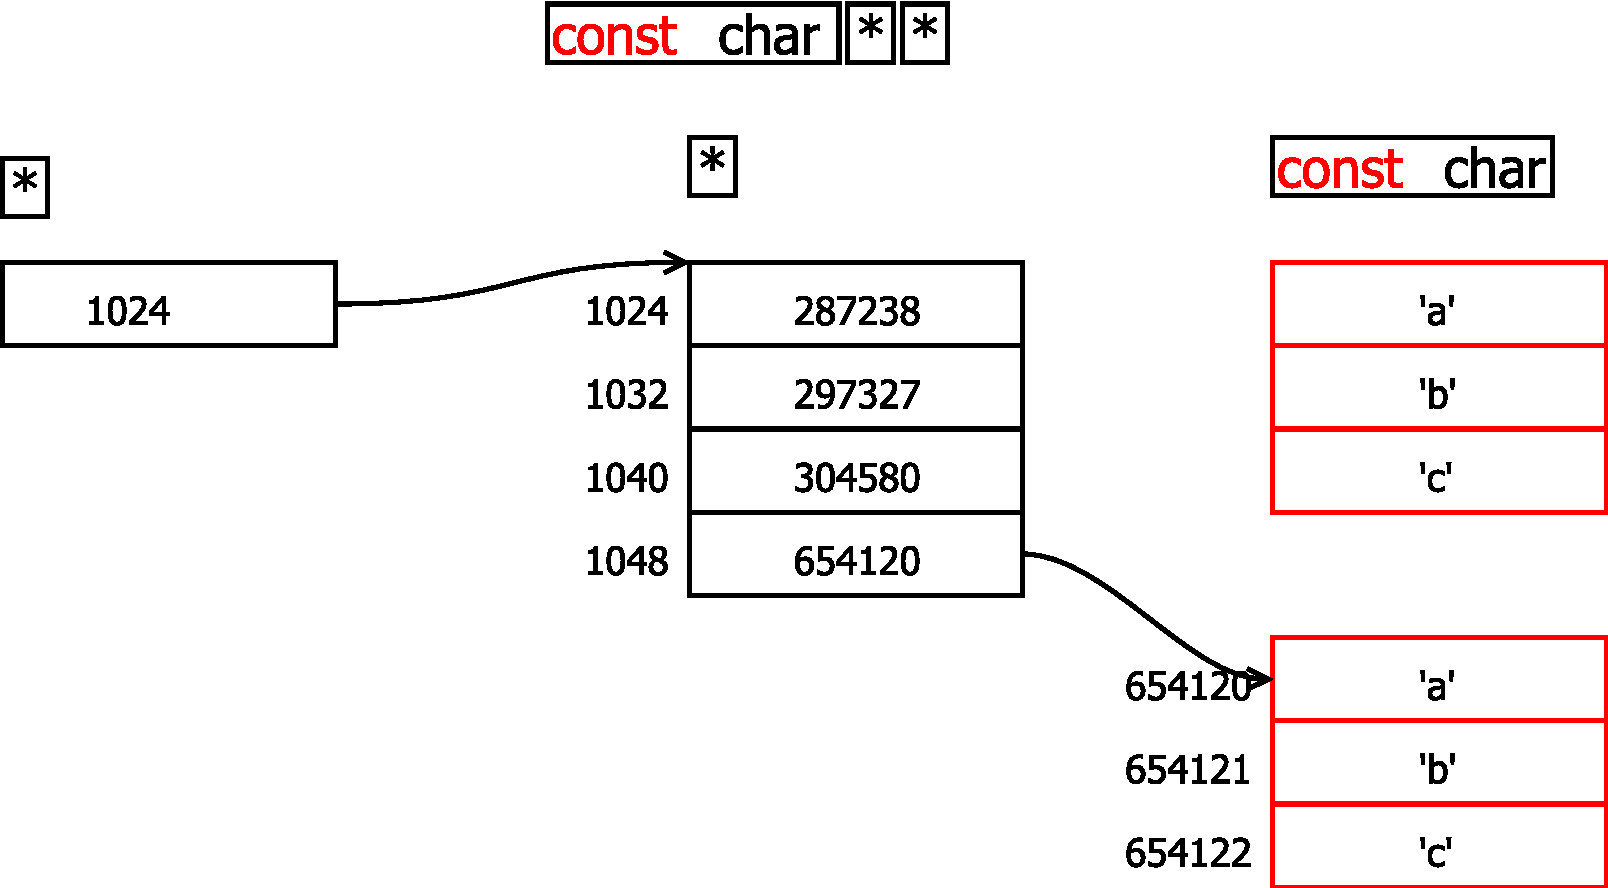
\includegraphics[width=\linewidth]{const_char_pointer_pointer}
    \caption{Pointer to pointer to constant \texttt{char}}
    \label{img:constcharpointerpointer}
\end{figure}

\begin{figure}[H]
    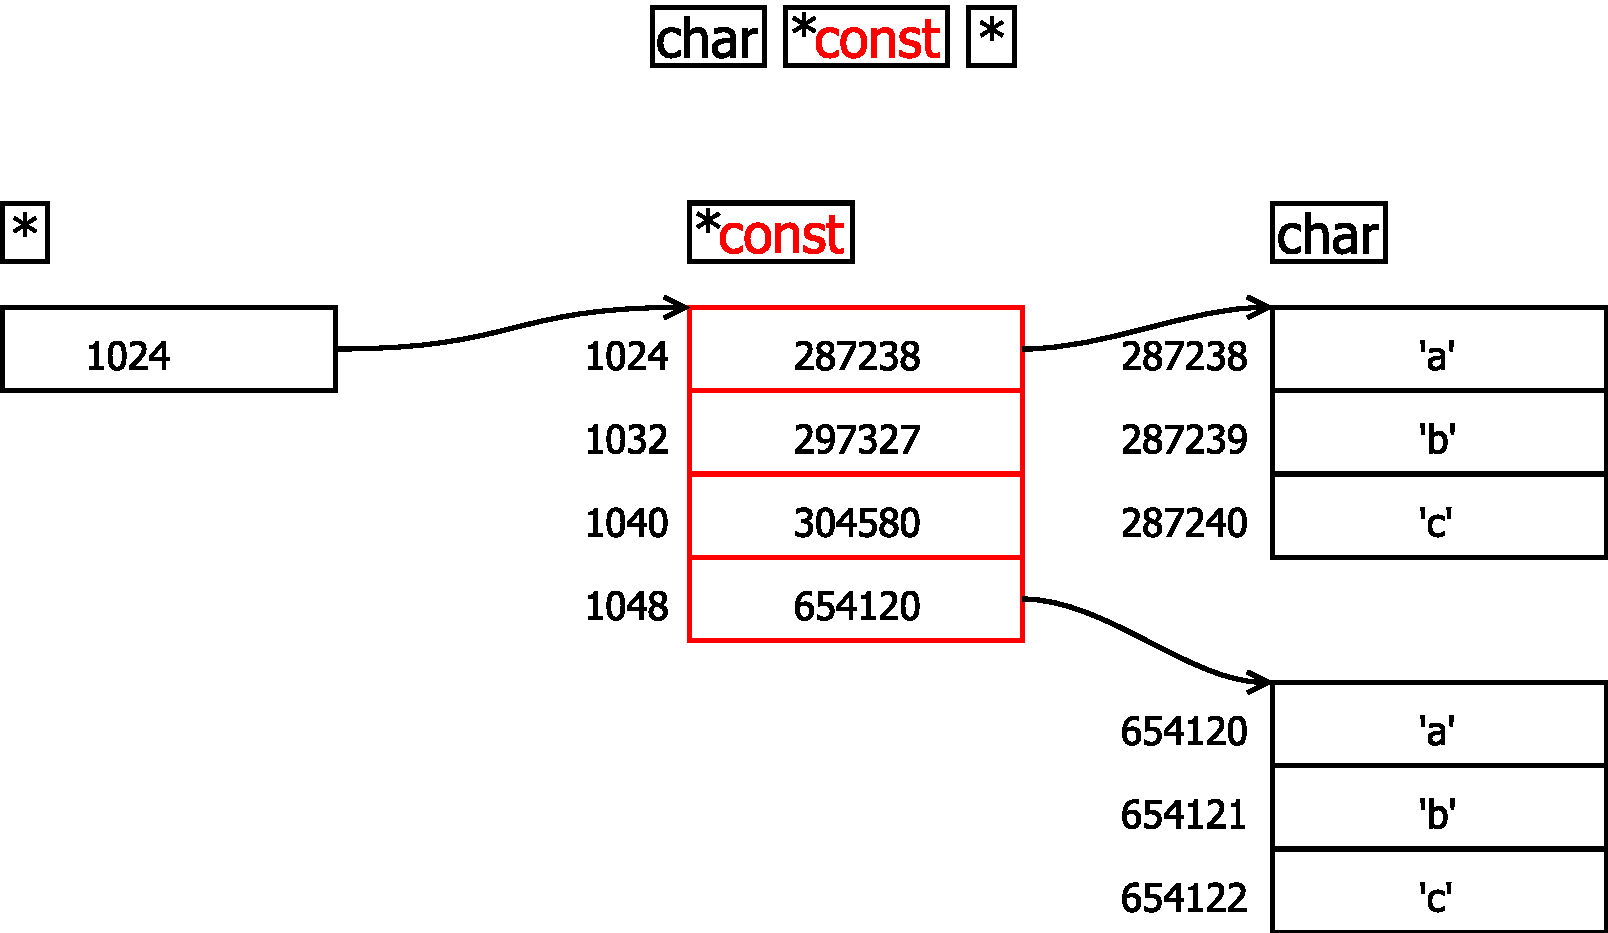
\includegraphics[width=\linewidth]{char_pointer_const_pointer}
    \caption{Pointer to constant pointer to \texttt{char}}
    \label{img:charconstpointerpointer}
\end{figure}

Let's explain it slowly, if you look at the first picture, it is ``what we are
used to'', each asterisk is a new pointer level, so you can read the declaration
from left to right and will build the types. Let's start: we find \verb"const",
what comes first is constant, after that, we know it is a \verb!char!, now it
comes an asterisk, the asterisk starts a new pointer level, so this pointer will
not be constant, because there is not \verb!const! to its right and, finally,
another pointer level, which isn't constant either. Now we have the three
groups, you invert them, which would be: non constant pointer to non constant
pointer to constant \verb!char!.

The next case we have is a \verb!char!, after it an asterisk, that is, a pointer
level, is has a \verb"const" on the right, so it is constant, and later another
pointer, without \verb"const". That is, inverting it: non constant pointer to
constant pointer to non constant \verb"char". In both cases, in the picture, I
have drawn in red the values you cannot change, as you can see, in the first one
we cannot change the strings, but we can change the intermediate pointers. In
the second case, on the contrary, we can modify the characters, but not the
pointers of the intermediate array.

One of the implications of the generic functions is, as I said before, a
decrease in the performance of the algorithms. I already mentioned the two
reasons that make this so. The first one is that using void pointers, some
calculations that could be done in an implicit way (like copying numbers from
one place to another, either integers or decimals) are done explicitly and byte
by byte. I am not going to dive into details of computer architecture, but
computers know how to copy packs of four of eight bytes fast, because they know
that's the size of integers and doubles (being able to do so with up to eight
bytes is one od the advantages of 64 bit computers). When we copy byte by byte,
we avoid this optimization and, also, we need to loop several times for copying
loops, which would be operators in other way. The other reason is that the
compiler has more information about the code when the functions are called
``as they are'', if they're in variables and passed ar arguments, it has less
information which makes the prgram slower. To make this visible, we are going to
perform a comparison between the specific version and the generic one, sorting
and array of 65.536 and 131.072 integers.

\begin{table}[H]
\begin{tabularx}{\linewidth}{|c|R|R|}
\hline
\textbf{Function}&\textbf{N=35.536}&\textbf{N=131.072}\\\hline
Specific&16.21&64.61\\\hline
Generic&41.20&164.44\\\hline
\textbf{Ratio}&0.39&0.39\\\hline
\end{tabularx}
\caption{Tiempos de ejecución de los distintos algoritmos}
\label{tab:sortingTimes}
\end{table}

As you can see, the generic version takes more time, but I have calculated the
ratio between the specific version and the generic one and you can see that
\textbf{it remains constant}. This means that, independently of the size of
the vector, it makes the generic algorithm scalable, which is a word used in
computing to say that the problem can be enlarged without the performance
declining. The conclusion is that, if you can take the performance hit in
general terms, you can implementing the generic version without the fear that
big problems are solved very slowly.

% Un ejercicio muy interesante sería que programaras la versión genérica de
% \textit{Quick Sort} y que, además, hicieras estas mismas mediciones. Para
% medir el tiempo puedes utilizar este código:

An interesting exercise would be that you wrote the generic version of Quick
Sort and that you also perform these measurements. To measure times you can use
this code:

\noindent
\begin{minipage}[H]{\linewidth}
\mbox{}
\begin{lstlisting}[style=C,
caption={How to measure time},
label={lst:measure_times}]
#include <stdio.h>
#include <time.h>

double timespec_to_double(const struct timespec* tm)
{
    return tm->tv_sec + tm->tv_nsec / 1000000000.0;
}

int main(int argc, char** argv)
{
    double start, stop;
    struct timespec start_ts, stop_ts;

    clock_gettime(CLOCK_REALTIME, &start_ts);
    start = timespec_to_double(&start_ts);
    // The code you can to measure here
    clock_gettime(CLOCK_REALTIME, &stop_ts);
    stop = timespec_to_double(&stop_ts);
    printf("Hemos tardado: %lf\n", stop - start);
}
\end{lstlisting}
\end{minipage}

The function \verb!clock_gettime! is a function to measure time in peculiar
mode, in Linux systems time is measured from January first 1970. Therefore,
the struct \verb!timespec! indicates the time elapsed since then as a number
of seconds plus the corresponding nanoseconds in the respective members. Since
this is not practical I have created a little function to translate that struct
to decimal number so you can substract it comfortably. After that, you can
measure the time before and after and later I substract the strart time from the
end time and I print it, as you can see.

\section{Complete example of program}
This section it at the end because we have seen each part of the language in
detail and by itself, in this one we're going to assemble all the pieces in a
big picture. To do so we're going to use and refine an aexample that has been
recurrent in the manual: the management of a struct that stores the data of a
person, but we're going to achieve to separate the user of the functions from
the internal functionality of the code.

What we will do is to create a file in source code called \verb!person.c! and
its corresponding header file, \verb!person.h!, in this file we will include
functionality to create a person struct, change its attributes, read them and
serialize them. Also, we're going to see and interesting artifact of the
language to avoid the user to change the internal fields of our structs. For
example: we assign pointers to memory zone that we do not control from this
functions that we're going to provide to manipulate the struct.


The first thing I am going to do is to create the header file because we have
already defined in a very concrete way the functionality of this source code.
Here is a very interesting thing, let's see the file.

\noindent
\begin{minipage}[H]{\linewidth}
\mbox{}
\begin{lstlisting}[style=C,
caption={Final example of program -- \texttt{person.h}},
label={lst:finalExPerson_h}]
#ifndef PERSON_H
#define PERSON_H

typedef struct person_s person_t;

person_t *create_person(const char *name, const char *last_name,
                        unsigned int age);

void destroy_person(person_t *p);

void person_set_name(person_t *p, const char *name);

void person_set_last_name(person_t *p, const char *last_name);

void person_set_age(person_t *p, unsigned int age);

const char *person_get_name(const person_t *person);

const char *person_get_last_name(const person_t *person);

unsigned int person_get_age(const person_t *person);

char *person_to_string(const person_t *p);

#endif
\end{lstlisting}
\end{minipage}

Here you can see one of the interesting things of this final example: we are
declaring the type \verb!person_t! but not the \verb!struct! it gives a name to,
this meand that any source code file that includes this header \textbf{wouldn't}
know the definition of the struct. This implies that the user of the header
will not be able to declare variable of this type, but he will be able to
declare pointers, because all pointers have the same size. If we tried to
declare a variable of this type, the compiler will throw an error like this one:

\noindent
\begin{minipage}[H]{\linewidth}
\mbox{}
\begin{lstlisting}[style=terminalStyle]
main.c: In function 'main':
main.c:5:14: error: storage size of 'francis' isn't known
    5 |     person_t francis;
      |              ^~~~~~~
\end{lstlisting}
\end{minipage}

This is the mechanism that allows us to avoid the user to change the content of
the struct outside of our control (as we commented in program
\ref{lst:structConstMain}) because, in the same we the user doesn't know the
size of the type, it doesn't know the members of this struct, so he can't
access them. Notice, also, since we haven't included any header in
\verb!person.h!. If we needed them, for example the header \verb!stdint.h!
contains definitions of useful types like those of standard size: \verb!int8_t!,
\verb!int16_t!, etc.; if we wanted to define some function with an argument of
these types or a function with a return type of these, it'd be needed to
include the header. If we needed them in the implementation (in the declaration
of struct, in the function definitions...), we will include those headers in the
source code (in the \verb!.c! file).

The next file is, precidely, this source code file: \verb!person.c!. This is
long, so I will include it in three sections: type declaration (which will
contain just one), the struct manipulation functions and, finally, the ones
to retrieve the information from the struct.

\noindent
\begin{minipage}[H]{\linewidth}
\mbox{}
\begin{lstlisting}[style=C, label={lst:finalExDefinition},
caption={Final example of program -- \texttt{person.c} definitions}]
#include <string.h> //strdup, memset
#include <stdlib.h> //malloc
#include <stdio.h>  //snprintf
#include "person.h"

struct person_s
{
    char *name;
    char *last_name;
    unsigned int age;
};

person_t *create_person(const char *name,
                        const char *last_name,
                        unsigned int age)
{
    person_t *res = malloc(sizeof(*res));
    memset(res, 0, sizeof(*res));

    res->age = age;
    res->name = strdup(name);
    res->last_name = strdup(last_name);

    return res;
}

void destroy_person(person_t *p)
{
    free(p->name);
    free(p->last_name);
    free(p);
}
\end{lstlisting}
\end{minipage}

Here we can see the definition of the type that in the header we renamed with
\verb!typedef!, this style of declaration of a type is called a forwarding
declaration. Here, apart from the proper type definition, we hace the functions
that create is and destroy it. Since this struct contains elements allocated
dynamically, we must provide the use a way to liberate the resources of the
struct. As you can see, in creation functions we allocate space
\textbf{for the very struct} and for its fields.

We must allocate ourselves dynamically the memory for the struct in addition
to the members because, remember, outside this file the source code file can't
declare anything but pointers, and that pointer will not have space for anything
if we do not allocate it. After that, we allocate memory for the content the
members of the struct point to. In the destruction function, simmetrically,
we free the the contents of the members and later the struct itself. Notice,
also how we have declared we could as constants, because in this way the user
will not doubt if we're going to modify the data he provides us with.

Las siguientes funciones son las que nos permiten sobreescribir los datos:

\noindent
\begin{minipage}[H]{\linewidth}
\mbox{}
\begin{lstlisting}[style=C, label={lst:finalExSetter},
caption={Final example of program -- \texttt{person.c} manipulation}]
void person_set_name(person_t *p, const char *name)
{
    free(p->name);
    p->name = strdup(name);
}

void person_set_last_name(person_t *p, const char *last_name)
{
    free(p->last_name);
    p->last_name = strdup(last_name);
}

void person_set_age(person_t *p, unsigned int age)
{
    p->age = age;
}
\end{lstlisting}
\end{minipage}

As you can see, the functions are simple, we free the memory of the members and
then we assign to them the duplication of the argument we have received. Again,
look at how we have defined as constant the arguments in the same way we did in
the creation. Functions do not return anything (\verb!void!) because it won't
have any sense. Although we could return an integer to act as an error code,
for example if the memory reserve failed, you could return a number less than
zero.

\noindent
\begin{minipage}[H]{\linewidth}
\mbox{}
\begin{lstlisting}[style=C, label={lst:finalExGetter},
caption={Final example of program -- \texttt{person.c} retrieval}]
const char *person_get_name(const person_t *p)
{
    return p->name;
}

const char *person_get_last_name(const person_t *person)
{
    return person->last_name;
}

unsigned int person_get_age(const person_t *person)
{
    return person->age;
}

char *person_to_string(const person_t *p)
{
#define MAX_STRING_SIZE ((unsigned int)1024)

    char res[MAX_STRING_SIZE + 1];
    snprintf(res, MAX_STRING_SIZE, "{\"name\":\"%s\","
                                   "\"last_name\":\"%s\","
                                   "\"age\":%u}",
             p->name, p->last_name, p->age);
    return strdup(res);
#undef MAX_STRING_SIZE
}
\end{lstlisting}
\end{minipage}

Here you must notice that we return constant pointer to \verb!char!, precisely
to avoid the user to free, manipulate or change the content of the fields of
the struct. Nevetherless; in the serialization function (which I have written in
the most simple way) I return a non constant pointer because the responsibility
of freeing the pointer is the user's, not of this library. Also, in this last
function you can see we can delete a macro with the directibe \verb!#undef!.
This is useful when you need to initialice an array, like here, but you do not
want to pollute the source code with symbols. Hence, if another function used
strings with other sizes, we could use the same name, like these macros being
a different variable. Again: be careful, macros work at a preprocessor level,
so you're not defining any new variable in the function, just a region in the
code where a symbol will be substituted by another.

Finally, in the main file we can use this functionality:

\noindent
\begin{minipage}[H]{\linewidth}
\mbox{}
\begin{lstlisting}[style=C, label={lst:finalExMain},
caption={Final example of program  -- \texttt{main.c}}]
#include "person.h"
#include <stdlib.h>
#include <stdio.h>

int main(void)
{
    person_t* person = create_person("John", "Smith", 18);

    char* serialization = person_to_string(person);

    printf("%s\n", serialization);
    free(serialization);

    person_set_name(person, "Michael");
    person_set_last_name(person, "Johnson");
    person_set_age(person, 33);

    serialization = person_to_string(person);
    printf("%s\n", serialization);
    free(serialization);
}
\end{lstlisting}
\end{minipage}

Here you can see how these struct with this design patter are used. First you
reserve them, later you use them, you can manipulate them, and, finally, you
liberate it, all of it done with the functions provided by the same library
that provided the struct. With this pattern, the user is less capable of
committing some errors.

Now, let's see quickly how this could be compiled, to remember it. Firstly we
will do it using object files and, later, we will create a dynamic library and
link it to the executable. To compile using the object files we will use these
steps.

\noindent
\begin{minipage}[H]{\linewidth}
\begin{enumerate}
\item Create the object code for \verb!person.c!.

\noindent
\begin{minipage}[H]{\linewidth}
\mbox{}
\begin{lstlisting}[style=terminalStyle]
\$ gcc -c person.c
\end{lstlisting}
\end{minipage}
\item Create the object code for \verb!main.c!.

\noindent
\begin{minipage}[H]{\linewidth}
\mbox{}
\begin{lstlisting}[style=terminalStyle]
\$ gcc -c main.c
\end{lstlisting}
\end{minipage}
\item Create the executable with both object codes.

\noindent
\begin{minipage}[H]{\linewidth}
\mbox{}
\begin{lstlisting}[style=terminalStyle]
\$ gcc -o main.exe main.o person.o -g -Wall -Wextra
\end{lstlisting}
\end{minipage}
\end{enumerate}
\end{minipage}

For the library, we will use these steps:

\noindent
\begin{minipage}[H]{\linewidth}
\begin{enumerate}
\item Create the object file of \verb!person.c!

\noindent
\begin{minipage}[H]{\linewidth}
\mbox{}
\begin{lstlisting}[style=terminalStyle]
\$ gcc -c person.c
\end{lstlisting}
\end{minipage}
\item Create a library with that object file:

\noindent
\begin{minipage}[H]{\linewidth}
\mbox{}
\begin{lstlisting}[style=terminalStyle]
\$ gcc -shared -o libperson.so person.o
\end{lstlisting}
\end{minipage}
\item Create the object code of \verb!main.c!

\noindent
\begin{minipage}[H]{\linewidth}
\mbox{}
\begin{lstlisting}[style=terminalStyle]
\$ gcc -c main.c
\end{lstlisting}
\end{minipage}
\item Create the executable using the library:

\noindent
\begin{minipage}[H]{\linewidth}
\mbox{}
\begin{lstlisting}[style=terminalStyle]
\$ gcc -L. -Wl,-rpath=. -o main.exe main.o -lperson
\end{lstlisting}
\end{minipage}
\end{enumerate}
\end{minipage}

In this final example we have seen examples of most of the concepts that have
been explained in the manual: variables, pointers, memory, dynamic allocation,
structs, macros, linking, compilation, constance and signedness. It is much
information in a few pages, but allows ut to have a global image of all that
has been explained before in detail.


\section{Annex A: exercises solutions}
\begin{exercises}
\item Escribe un programa y declara en él una estructura que defina un círculo
en dos dimensiones (su centro y su radio). Y haz que el programa declare una
variable de ese tipo y calcule su área.


\noindent
\begin{minipage}[H]{\linewidth}
\mbox{}
\begin{lstlisting}[style=C,
caption={Solución al ejercicio 1},
label={lst:solution1}]
#include <stdio.h>

struct circle_s {
    double x;
    double y;
    double r;
};

int main(void)
{
    struct circle_s circle = { 1 , 1 , 3.4 };
    double area = 3.141592 * circle.r * circle.r;
    printf("El área del círculo en el punto [%f, %f] con un radio de % f es: %f\n", circle.x, circle.y, circle.r, area);
}
\end{lstlisting}
\end{minipage}

\item Haz un programa que, basándose en el struct punto presentado en el
ejemplo, declare e inicialice un array de ellos y vaya diciendo las direcciones
que hay que seguir para ir de uno a otro.


\noindent
\begin{minipage}[H]{\linewidth}
\mbox{}
\begin{lstlisting}[style=C,
caption={Solución al ejercicio 2},
label={lst:solution2}]
#include <stdio.h>
struct point_s {
    double x;
    double y;
};

int main(void)
{
    struct point_s points[10] = { {-1.056171, 3.401877},
                                  {2.984400, 2.830992},
                                  {-3.024486, 4.116474},
                                  {2.682296, -1.647772},
                                  {0.539700, -2.222253},
                                  {1.288709, -0.226029},
                                  {0.134009, -1.352155},
                                  {4.161951, 4.522297},
                                  {2.172969, 1.357117},
                                  {1.069689, -3.583974} };

    for(int ii = 1; ii < 10; ++ii){
        if (points[ii - 1].x < points[ii].x) {
            printf("Derecha");
        }else if(points[ii - 1].x == points[ii].x){
            printf("Quieto");
        }else if(points[ii - 1].x > points[ii].x){
            printf("Izquierda");
        }
        printf(", ");
        if (points[ii - 1].y < points[ii].y) {
            printf("Arriba");
        }else if(points[ii - 1].y == points[ii].y){
            printf("Quieto");
        }else if(points[ii - 1].y > points[ii].y){
            printf("Abajo");
        }
        printf("\n");
    }
}
\end{lstlisting}
\end{minipage}

\item Haz un programa que declare un array bidimensional y calcule la suma de
sus filas y sus columnas.


\noindent
\begin{minipage}[H]{\linewidth}
\mbox{}
\begin{lstlisting}[style=C,
caption={Solución al ejercicio 3},
label={lst:solution3}]
#include <stdio.h>

int main(void)
{
    int array[3][3] = { {1,3,6},{7,3,6},{1,2,4} };

    for (int ii = 0; ii < 3; ++ii) {
        for (int jj = 0; jj < 3; ++jj) {
            printf("%d ", array[ii][jj]);
        }
        int suma = 0;
        for(int jj = 0; jj < 3; ++jj){
            suma += array[ii][jj];
        }
        printf("= %d\n", suma);
    }
    for(int ii = 0; ii < 3*2; ++ii){
        printf("-");
    }
    printf("\n");
    for(int ii = 0; ii < 3; ++ii){
        int suma = 0;
        for(int jj = 0; jj < 3; ++jj){
            suma+=array[jj][ii];
        }
        printf("%d ", suma);
    }
    printf("\n");
}

\end{lstlisting}
\end{minipage}


\item Haz un programa que haga lo siguiente para los números del 1 al 100 ambos
incluidos: si el número es divisible entre 2, debe imprimirse por pantalla
<<fizz>>, si es divisible entre 5, <<buzz>>, y si es divisible entre los dos,
<<fizzbuzz>>, no imprimir nada en otro caso.


\noindent
\begin{minipage}[H]{\linewidth}
\mbox{}
\begin{lstlisting}[style=C,
caption={Solución al ejercicio 4},
label={lst:solution4}]
#include <stdio.h>

int main(void)
{
    for (int ii = 1; ii <= 100; ++ii){
        int end_of_line = 0;
        if (ii % 2 == 0){
            printf("fizz");
            end_of_line = 1;
        }

        if(ii % 5 == 0){
            printf("buzz");
            end_of_line = 1;
        }
        if(end_of_line){
            printf("\n");
        }
    }
}
\end{lstlisting}
\end{minipage}

\item Escribe una función que calcule si un número es primo o no.


\noindent
\begin{minipage}[H]{\linewidth}
\mbox{}
\begin{lstlisting}[style=C,
caption={Solución al ejercicio 5},
label={lst:solution5}]
#include <stdio.h>

int is_prime(int number) {
    int prime = 1;
    for (int ii = 2; ii < number / 2 && prime; ++ii) {
        if (0 == number % ii) {
            prime = 0;
        }
    }
    return prime;
}

int main(void)
{
    for(int ii = 2; ii < 100; ii++){
        printf("El número %d ", ii);
        if(is_prime(ii)){
            printf("es primo.");
        }else{
            printf("no es primo");
        }
        printf("\n");
    }
}
\end{lstlisting}
\end{minipage}

\item Escribe una función que calcule la distancia entre dos estructuras punto
de las usadas en la sección anterior.


\noindent
\begin{minipage}[H]{\linewidth}
\mbox{}
\begin{lstlisting}[style=C,
caption={Solución al ejercicio 6},
label={lst:solution6}]
#include <stdio.h>
#include <math.h>
struct point_s {
    double x;
    double y;
};

double distance(struct point_s a, struct point_s b) {
    double res = 0.0;
    double diff_x = a.x - b.x;
    double diff_y = a.y - b.y;
    res = sqrt(diff_x * diff_x + diff_y * diff_y);
    return res;
}

int main(void)
{
    struct point_s a = {1.2, 4.3};
    struct point_s b = {3.4, 5.5};
    printf("La distancia entre [%f, %f] y [%f, %f] es: %f\n", a.x, a.y, b.x, b.y, distance(a,b));
}
\end{lstlisting}
\end{minipage}

\item Escribe una función que reciba un array de enteros y un caracter separador
que imprima los elementos del array separados por ese caracter.


\noindent
\begin{minipage}[H]{\linewidth}
\mbox{}
\begin{lstlisting}[style=C,
caption={Solución al ejercicio 7},
label={lst:solution7}]
#include <stdio.h>
void print_separated(int array[], int array_size, char separator){
    for(int ii = 0; ii < array_size; ++ii){
        printf("%d%c", array[ii], separator);
    }
}

int main(void)
{
    int my_array[] = {1,2,3,4,5,6,7,8,9,0};
    print_separated(my_array, 10, '|');
    printf("\n");
}
\end{lstlisting}
\end{minipage}

\item Escribe una función que encapsule el programa
\ref{lst:linealSystemFinal}: \nameref{lst:linealSystemFinal}.
La función debe recibir los coeficientes de las ecuaciones
($a$, $b$, $c$, $d$, $e$ y $f$). Puede recibirlos por separado o en un array.
Para devolver el resultado puedes crear una estructura que simplemente tenga
dos \verb!double!.



\begin{lstlisting}[style=C,
caption={Solución al ejercicio 8},
label={lst:solution8}]
#include <stdio.h>

struct solution_s {
    double x;
    double y;
    int solved;
};

struct solution_s linear_system(int a, int b, int c, int d, int e, int f) {

    double divisor;
    struct solution_s res;
    res.solved = 1;
    if (a != 0 && d != 0) {
        divisor = (a * e - d * b);
        if (divisor == 0)
        {
            printf("El sistema es irresoluble .\n");
            res.solved = 0;
        }
        else
        {
            res.y = (a * f - d * c) / divisor;
            res.x = (f - e * res.y) / (d);
        }
    }
    else if (b != 0 && e != 0) {
        divisor = (b * d - e * a);
        if (divisor == 0) {
            printf("El sistema es irresoluble .\n");
            res.solved = 0;
        }
        else {
            res.x = (b * f - e * c) / divisor;
            res.y = (c - a * res.x) / b;
        }
    }
    else if ((a == 0 && b == 0) || (d == 0 && e == 0)) {
        printf(" Esto no es un sistema \n");
        res.solved = 0;
    }
    else {
        if (a != 0) {
            res.x = (double)c / a;
            res.y = (double)f / e;
        }
        else {
            res.x = (double)f / d;
            res.y = (double)c / b;
        }
    }
    return res;
}


int main(void)
{
    struct solution_s sol = linear_system(1, 1, 1, 2, 2, 2);
    printf(" %dx+ %dy= %d\n", 1, 2, 3);
    printf(" %dx+ %dy= %d\n", 4, 5, 6);
    if (sol.solved) {
        printf("x = %f; y = %f\n", sol.x, sol.y);
    }
    else {
        printf("El sistema no tiene solucion.\n");
    }
}
\end{lstlisting}


\item Escribe una función que normalice los elementos de un array de
\verb!double!.

\noindent
\begin{minipage}[H]{\linewidth}
\mbox{}
\begin{lstlisting}[style=C,
caption={Solución al ejercicio 9},
label={lst:solution9}]
#include <stdio.h>

void normalize(double array[], int array_size) {
    double biggest = array[0];
    for (int ii = 1; ii < array_size; ++ii) {
        if (array[ii] > biggest) {
            biggest = array[ii];
        }
    }
    for (int ii = 0; ii < array_size; ++ii) {
        array[ii] /= biggest;
    }
}

int main(void)
{
    double array[] = { 1,2,3,4,5,6,7,8,9,10 };
    normalize(array, 10);
    for(int ii = 0; ii < 10; ++ii){
        printf("%f\n", array[ii]);
    }
    printf("\n");
}
\end{lstlisting}
\end{minipage}

\item Completa esta tabla de números en diferentes bases numéricas:
\begin{table}[H]
\begin{tabularx}{\linewidth}{|R|R|R|}
\hline
\multicolumn{1}{|Y|}{\textbf{Decimal}}& \multicolumn{1}{Y|}{\textbf{Binario}} & \multicolumn{1}{Y|}{\textbf{Hexadecimal}} \\\hline
73& 0100~1001 & 0x049 \\\hline
 38&0010~0110&0x026 \\\hline
303&0001~0010~1111&0x12F       \\\hline
128&1000~0000&0x080 \\\hline
\end{tabularx}
\end{table}
\item Vuelve al ejercicio noveno y reproduce los contenidos de la pila en cada
bloque de código del programa. Utiliza de referencia la solución que propongo
yo.

\begin{stack}
    \item Función main
    \begin{stack}
        \item Array (10 elementos)
        \item Entramos en la función normalize
        \begin{stack}
            \item Array (puntero a)
            \item \verb!array_size!
            \item \verb!biggest!
            \item Primer bucle for
            \begin{stack}
                \item \verb!ii!
            \end{stack}
            \item Segundo bucle for
            \begin{stack}
                \item \verb!ii!
            \end{stack}
        \end{stack}
        \item Bucle for
        \begin{stack}
            \item \verb!ii!
        \end{stack}
    \end{stack}
\end{stack}

\item Haz un programa que cree un puntero de tres niveles de tipo \verb!int!,
lo reserve correctamente, lo rellene con el valores correlativos
\textbf{empezando en uno} y después lo imprima de una manera comprensible.
Finalmente, libéralo también de tal modo que no quede memoria sin liberar al
final del programa.

\noindent
\begin{minipage}[H]{\linewidth}
\mbox{}
\begin{lstlisting}[style=C,label=lst:solution12, caption={Solución al ejercicio 12}]
#include <stdio.h>
#include <stdlib.h>

#define DEPTH (10)
#define WIDTH (5)
#define HEIGHT (12)

int main(int argc, char const *argv[]) {
    int ***cube = malloc(sizeof(*cube) * DEPTH);

    for (int ii = 0; ii < DEPTH; ++ii) {
        cube[ii] = malloc(sizeof(**cube) * HEIGHT);
        for (int jj = 0; jj < HEIGHT; ++jj) {
            cube[ii][jj] = malloc(sizeof(***cube) * WIDTH);
            for (int kk = 0; kk < WIDTH; ++kk) {
                cube[ii][jj][kk] =
                    kk + jj * WIDTH + ii * HEIGHT * WIDTH + 1;
            }
        }
    }

    for (int ii = 0; ii < DEPTH; ++ii) {
        for (int jj = 0; jj < HEIGHT; ++jj) {
            for (int kk = 0; kk < WIDTH; ++kk) {
                printf("%3d ", cube[ii][jj][kk]);
            }
            printf("\n");
        }
        printf("\n");
    }

    for (int ii = 0; ii < DEPTH; ++ii) {
        for (int jj = 0; jj < HEIGHT; ++jj) {
            free(cube[ii][jj]);
        }
        free(cube[ii]);
    }
    free(cube);

    return 0;
}
\end{lstlisting}
\end{minipage}


\item Basándote en el programa anterior, crea dos funciones, una para crear
una matriz tridimensional con memoria dinámica dadas sus tres dimensiones y
otra para liberarla.

\noindent
\begin{minipage}[H]{\linewidth}
\mbox{}
\begin{lstlisting}[ style=C,
                    label=lst:solution12,
                    caption={Solución al ejercicio 13 -- reserva}]
int ***malloc_cube(size_t depth, size_t height, size_t width) {
    int ***cube = malloc(sizeof(*cube) * depth);

    for (int ii = 0; ii < depth; ++ii) {
        cube[ii] = malloc(sizeof(**cube) * height);
        for (int jj = 0; jj < height; ++jj) {
            cube[ii][jj] = malloc(sizeof(***cube) * width);
            for (int kk = 0; kk < width; ++kk) {
                cube[ii][jj][kk] =
                    kk + jj * width + ii * height * width + 1;
            }
        }
    }
    return cube;
}
\end{lstlisting}
\end{minipage}

\noindent
\begin{minipage}[H]{\linewidth}
\mbox{}
\begin{lstlisting}[ style=C,
                    label=lst:solution12,
                    caption={Solución al ejercicio 13 -- impresión}]
void print_cube(int ***cube, size_t depth, size_t height,
                size_t width) {
    for (int ii = 0; ii < depth; ++ii) {
        for (int jj = 0; jj < height; ++jj) {
            for (int kk = 0; kk < width; ++kk) {
                printf("%3d ", cube[ii][jj][kk]);
            }
            printf("\n");
        }
        printf("\n");
    }
}
\end{lstlisting}
\end{minipage}

\noindent
\begin{minipage}[H]{\linewidth}
\mbox{}
\begin{lstlisting}[ style=C,
                    label=lst:solution12,
                    caption={Solución al ejercicio 13 -- liberación}]
void free_cube(int ***cube, size_t depth, size_t height,
               size_t width) {
    for (int ii = 0; ii < depth; ++ii) {
        for (int jj = 0; jj < height; ++jj) {
            free(cube[ii][jj]);
        }
        free(cube[ii]);
    }
    free(cube);
}
\end{lstlisting}
\end{minipage}

\noindent
\begin{minipage}[H]{\linewidth}
\mbox{}
\begin{lstlisting}[ style=C,
                    label=lst:solution12,
                    caption={Solución al ejercicio 13 -- función \texttt{main}}]
int main(int argc, char const *argv[]) {
    int ***cube = malloc_cube(DEPTH, HEIGHT, WIDTH);
    print_cube(cube, DEPTH, HEIGHT, WIDTH);
    free_cube(cube, DEPTH, HEIGHT, WIDTH);
}
\end{lstlisting}
\end{minipage}

\item Escribe un programa que reciba un número variable de números como
argumentos e imprima la descomposición en factores primos de todo ellos.
Se recomienda hacer control de errores comprobando que los argumentos son
números antes de utilizarlos, etc.

\noindent
\begin{minipage}[H]{\linewidth}
\mbox{}
\begin{lstlisting}[ style=C,
                    label=lst:solution12,
                    caption={Solución al ejercicio 13 -- función \texttt{main}}]
int main(int argc, char const *argv[]) {
    int ***cube = malloc_cube(DEPTH, HEIGHT, WIDTH);
    print_cube(cube, DEPTH, HEIGHT, WIDTH);
    free_cube(cube, DEPTH, HEIGHT, WIDTH);
}
\end{lstlisting}
\end{minipage}

\item Escribe un programa que lea \textbf{por consola} una serie de palabras
y que sólo deje de leer cuando se introduzca <<!!>> como palabra. Después, debe
imprimir dichas palabras en orden aleatorio. La función \verb!rand! devuelve
un número aleatorio entre cero y el máximo entero positivo. Si quieres que
devuelva números aleatorios \textbf{distintos} cada vez debes ejecutar
\verb!srand(time(NULL));! al inicio de la función \verb!main!. Debes incluir la
cabecera \verb!time.h!.

\noindent
\begin{minipage}[H]{\linewidth}
\mbox{}
\begin{lstlisting}[ style=C,
                    label=lst:solution12,
                    caption={Solución al ejercicio 15}]
#include <stdio.h>
#include <stdlib.h>
#include <string.h>
#include <time.h>

#define STRING_SIZE (1024)
#define MAX_WORDS (1024)

int main(int argc, char const *argv[]) {
    char *word_set[1024];
    int word_length = 0;
    do {
        word_set[word_length] = malloc(STRING_SIZE);
        scanf("%s", word_set[word_length]);
        word_length++;
    } while (strcmp(word_set[word_length - 1], "!!"));

    srand(time(NULL));
    for (int ii = 0; ii < word_length - 1; ++ii) {
        char *aux            = word_set[ii];
        int rand_index       = rand() % (word_length - 1);
        word_set[ii]         = word_set[rand_index];
        word_set[rand_index] = aux;
    }
    for (int ii = 0; ii < word_length - 1; ++ii) {
        printf("%s\n", word_set[ii]);
        free(word_set[ii]);
    }
    free(word_set[word_length-1]);
}
\end{lstlisting}
\end{minipage}

Como nota, para <<barajar>> el vector de palabras lo que hago el recorrerlo
intercambiando cada palabra con una posición aleatoria. Hay otros métodos
que quizás hayas usado como generar una posición aleatoria del vector y copiarlo
a otro, el problema de esto es que si lo que haces es generar un índice nuevo
cuando encuentras que ya has copiado ese, el número de veces que ejecutas
el aleatorio es, lógicamente, impredecible. Tal y como lo he escrito yo el
algoritmo siempre tardará lo mismo generando resultados moderadamente
aleatorios.

\item Haz una función que lea dos archivos e \textbf{intercambie} su contenido,
escribe dicho programa de tal modo que no sea necesario alojar ninguno de los
dos archivos en memoria completamente.

\newpage
\begin{lstlisting}[ style=C,
                    label=lst:solution16,
                    caption={Solución al ejercicio 16}]
#include <stdio.h>
#include <stdlib.h>

int main(int argc, char const *argv[]) {
    FILE *file_1 = NULL, *file_2 = NULL, *file_aux = NULL;
    const int BLOCK_SIZE = 1024;
    int read             = 0;
    char buffer[BLOCK_SIZE], aux_file_path[] = "/tmp/auxFile.txt";
    if (argc < 3) {
        printf("Uso: main.exe <archivo1> <archivo2>\n");
        return EXIT_FAILURE;
    }

    file_1 = fopen(argv[1], "r+");
    if (NULL == file_1) {
        printf("ERROR: El primer archivo no existe.\n");
        return EXIT_FAILURE;
    }

    file_2 = fopen(argv[2], "r+");
    if (NULL == file_2) {
        printf("ERROR: El segundo archivo no existe.\n");
        fclose(file_1);
        return EXIT_FAILURE;
    }

    file_aux = fopen(aux_file_path, "w+");
    if (NULL == file_aux) {
        fclose(file_1);
        fclose(file_2);
        return EXIT_FAILURE;
    }

    // copy file 1 to aux
    while (read = fread(buffer, sizeof(char), BLOCK_SIZE, file_1)) {
        fwrite(buffer, sizeof(char), read, file_aux);
    }
    fclose(file_1);
    file_1 = fopen(argv[1], "w+");
    if (NULL == file_1) {
        printf("Error, el primer archivo no se ha podido reabrir\n");
    }

    // copy file 2 to 1
    while (read = fread(buffer, sizeof(char), BLOCK_SIZE, file_2)) {
        fwrite(buffer, sizeof(char), read, file_1);
    }

    fclose(file_2);
    file_2 = fopen(argv[2], "w+");
    if (NULL == file_2) {
        printf("Error, el segundo archivo no se ha podido reabrir\n");
    }

    // copy aux file to file 2, we need to go back to begin of file aux
    fseek(file_aux, 0, SEEK_SET);
    while (read = fread(buffer, sizeof(char), BLOCK_SIZE, file_aux)) {
        fwrite(buffer, sizeof(char), read, file_2);
    }

    fclose(file_1);
    fclose(file_2);
    fclose(file_aux);
    remove(aux_file_path);
}
\end{lstlisting}

\item Escribe una función que reciba una palabra como argumento e indique
en qué posición (en bytes) dentro del archivo se encuentra la palabra. Sólo
tienes que dar la primera ocurrencia, si la palabra no se encuentra, devuelve
un número negativo. Haz un programa que, con esa función, reciba una ruta a un
archivo y una palabra e imprima el resultado de buscar la palabra en el archivo.

\noindent
\begin{minipage}[H]{\linewidth}
\mbox{}
\begin{lstlisting}[style=C,
caption={Solución al ejercicio 17},
label={lst:solution17}]
#include <stdio.h>
#include <stdlib.h>
#include <string.h>

int find_in_file(const char *path, const char *word) {
    FILE *file = NULL;
    char *buffer;
    int word_length = 0, read = 0, pos = -1;

    file = fopen(path, "r+");
    if (NULL == file) {
        printf("ERROR: El archivo no existe.\n");
        return -1;
    }
    word_length = strlen(word);
    buffer      = malloc(sizeof(char) * word_length * 2);

    while (read = fread(buffer, sizeof(char), word_length * 2, file)) {
        fseek(file, word_length - read, SEEK_CUR);
        for (int ii = 0; ii < word_length; ++ii) {
            char local_word[word_length + 1];
            memcpy(local_word, buffer + ii, word_length);
            local_word[word_length] = 0;
            if (!strcmp(local_word, word)) {
                pos = ftell(file) + ii - word_length;
                goto end;
            }
        }
    }
end:
    free(buffer);
    fclose(file);
    return pos;
}

int main(int argc, char const *argv[]) {

    int pos = find_in_file(argv[1], argv[2]);
    printf("La palabra %s está en la posición %d en el archivo %s\n",
           argv[2], pos, argv[1]);
}
\end{lstlisting}
\end{minipage}

Aquí puedes ver un uso típico de la instrucción \verb!goto!, como necesitamos
hacer lo mismo encontremos la palabra o no, lo que hacemos es establecer
una etiqueta y saltar allí para liberar recursos y devolver el resultado.

\item Reescribe el ejercicio 15 prescindiendo del array estático de punteros
a \verb!char!. (Usa \verb!realloc! y \verb!strdup!.

\noindent
\begin{minipage}[H]{\linewidth}
\mbox{}
\begin{lstlisting}[style=C,
caption={Solución al ejercicio 18},
label={lst:solution18}]
#include <stdio.h>
#include <stdlib.h>
#include <string.h>
#include <time.h>

int main(int argc, char const *argv[]) {
    char word[1024];
    char **word_set = NULL;
    int word_length = 0;
    do {
        word_set = realloc(word_set, ++word_length * sizeof(char *));
        scanf("%s", word);
        word_set[word_length - 1] = strdup(word);
    } while (strcmp(word, "!!"));

    srand(time(NULL));
    for (int ii = 0; ii < word_length - 1; ++ii) {
        char *aux            = word_set[ii];
        int rand_index       = rand() % (word_length - 1);
        word_set[ii]         = word_set[rand_index];
        word_set[rand_index] = aux;
    }
    for (int ii = 0; ii < word_length - 1; ++ii) {
        printf("%s\n", word_set[ii]);
    }
    for (int ii = 0; ii < word_length; ++ii) {
        free(word_set[ii]);
    }
    free(word_set);
}
\end{lstlisting}
\end{minipage}


\item Escribe un programa que reciba un número indeterminado de palabras como
argumentos y los ordene alfabéticamente y que, después, los imprima.


\noindent
\begin{minipage}[H]{\linewidth}
\mbox{}
\begin{lstlisting}[style=C,
caption={Solución al ejercicio 19},
label={lst:solution19}]
void generic_swap(void *one, void *other, size_t type_size) {
//...

void generic_bubble_sort(void *array, size_t array_size,
//...

int compare_strings(const void *one, const void *two) {
//...

int compare_strings(const void* one, const void* two) {
//...

int main(int argc, char const *argv[]) {

    generic_bubble_sort(argv + 1, argc - 1, sizeof(char *),
                        compare_strings);

    for (int ii = 1; ii < argc; ++ii) {
        printf("%s\n", argv[ii]);
    }
}
\end{lstlisting}
\end{minipage}

He usado las funciones de ejemplo para ordenar, así que omito su contenido,
simplemente tenemos que utilizar el comparador adecuado y tener en cuenta que
el primer argumento es el nombre de programa, que no queremos ordenar. Además,
puedes ver que podemos modificar el orden de los argumentos, pero no su
contenido, al haber declarado \texttt{argv} como \verb!char const*argv[]! que
quiere decir un array (puntero) no constante a \verb!char! constante. Es decir,
como ya vimos en la figura \ref{img:constcharpointerpointer}.


\item Haz un programa que reciba como argumento una palabra y un número. Si el
número es cero, debe convertir la palabra a minúscula, si el número es distinto
de cero, debe convertirla a mayúscula.

\noindent
\begin{minipage}[H]{\linewidth}
\mbox{}
\begin{lstlisting}[style=C,
caption={Solución al ejercicio 20},
label={lst:solution20}]
#include <stdio.h>
#include <stdlib.h>

char char_to_upper_case(char c) {
    if (c < 123 && c > 96) {
        return c - 32;
    }
    return c;
}

char char_to_lower_case(char c) {
    if (c < 91 && c > 64) {
        return c + 32;
    }
    return c;
}

char string_to_upper_case(char *message) {
    int length = strlen(message);
    for (int ii = 0; ii < length; ++ii) {
        message[ii] = char_to_upper_case(message[ii]);
    }
}

char string_to_lower_case(char *message) {
    int length = strlen(message);
    for (int ii = 0; ii < length; ++ii) {
        message[ii] = char_to_lower_case(message[ii]);
    }
}

int main(int argc, char const *argv[]) {

    char *message = strdup(argv[1]);
    int code = atoi(argv[2]);
    if(code){
        string_to_upper_case(message);
    }else{
        string_to_lower_case(message);
    }
    printf("%s\n", message);
    free(message);
}
\end{lstlisting}
\end{minipage}

Aquí hemos utilizado dos funciones diferentes para poner a mayúscula y
minúscula, otra opción sería utilizar un parámetro lógico (o incluso un
enumerado) para indicar qué tipo de letras se quiere y llamar a una función
que reciba ese parámetro y actúe en consecuencia. Puedes implementarlo así
como ejercicio extra.

\item Crea un programa que dado un número como argumento imprima una pirámide
como esta de tantos pisos como el número indicado.

\noindent
\begin{minipage}[H]{\linewidth}
\mbox{}
\begin{lstlisting}[style=C,
caption={Solución al ejercicio 21},
label={lst:solution21}]
#include <stdio.h>
#include <stdlib.h>
#include <string.h>

char **make_pyramid(int steps) {
    char **result = malloc(sizeof(*result) * steps);
    for (int ii = 0; ii < steps; ++ii) {
        result[ii] = malloc(sizeof(**result) * (steps * 2));
        memset(result[ii], ' ', steps * 2 - 1);
        memset(result[ii] + ii, '%', (steps * 2 - 1) - 2 * ii);
        result[ii][(steps - 1) * 2 + 1] = 0;
    }
    return result;
}

void free_pyramid(char **pyramid, int steps) {
    for (int ii = 0; ii < steps; ++ii) {
        free(pyramid[ii]);
    }
    free(pyramid);
}

int main(int argc, char const *argv[]) {
    int steps      = atoi(argv[1]);
    char **pyramid = make_pyramid(steps);
    for (int ii = 0; ii < steps; ++ii) {
        printf("%s\n", pyramid[ii]);
    }
    free_pyramid(pyramid, steps);
}
\end{lstlisting}
\end{minipage}




\item Escribe un programa que reciba una serie de puntos y de nombres para
cada uno y después los imprima en orden de su distancia al origen de menor a
mayor.

\noindent
\begin{minipage}[H]{\linewidth}
\mbox{}
\begin{lstlisting}[style=C,
caption={Solución al ejercicio 23 -- \texttt{tagged\_point.h}},
label={lst:solution23}]
#ifndef TAGGED_POINT_H
#define TAGGED_POINT_H
typedef struct tagged_point_s tagged_point_t;

tagged_point_t *tagged_point_create(const char *tag, double x,
                                    double y);

void tagged_point_set_tag(const char *tag, tagged_point_t *tp);

void tagged_point_set_x(double x, tagged_point_t *tp);

void tagged_point_set_y(double y, tagged_point_t *tp);

const char *tagged_point_get_tag(const tagged_point_t *tp);

double tagged_point_get_x(const tagged_point_t *tp);

double tagged_point_get_y(const tagged_point_t *tp);

void tagged_point_destroy(tagged_point_t *tp);

double tagged_point_distance(const tagged_point_t *a,
                             const tagged_point_t *b);
#endif
\end{lstlisting}
\end{minipage}

\noindent
\begin{minipage}[H]{\linewidth}
\mbox{}
\begin{lstlisting}[style=C,
caption={Solución al ejercicio 22 -- \texttt{tagged\_point.c}},
label={lst:solution22}]
#include "tagged_point.h"
#include <math.h>
#include <stdlib.h>
#include <string.h>

struct tagged_point_s {
    char *tag;
    double x, y;
};

tagged_point_t *tagged_point_create(const char *tag, double x,
                                    double y) {
    tagged_point_t *res = malloc(sizeof(tagged_point_t));
    res->x              = x;
    res->y              = y;
    res->tag            = strdup(tag);
}

void tagged_point_set_tag(const char *tag, tagged_point_t *tp) {
    free(tp->tag);
    tp->tag = strdup(tag);
}

void tagged_point_set_x(double x, tagged_point_t *tp) { tp->x = x; }

void tagged_point_set_y(double y, tagged_point_t *tp) { tp->y = y; }

const char *tagged_point_get_tag(const tagged_point_t *tp) {
    return tp->tag;
}

double tagged_point_get_x(const tagged_point_t *tp) { return tp->x; }

double tagged_point_get_y(const tagged_point_t *tp) { return tp->y; }

void tagged_point_destroy(tagged_point_t *tp) {
    free(tp->tag);
    free(tp);
}

double tagged_point_distance(const tagged_point_t *a,
                             const tagged_point_t *b) {
    tagged_point_t origin = {"origin", 0.0, 0.0};
    if (NULL == a) {
        a = &origin;
    }
    if (NULL == b) {
        b = &origin;
    }
    return sqrt((a->x - b->x) * (a->x - b->x) +
                (a->y - b->y) * (a->y - b->y));
}
\end{lstlisting}
\end{minipage}

\noindent
\begin{minipage}[H]{\linewidth}
\mbox{}
\begin{lstlisting}[style=C,
caption={Solución al ejercicio 22 -- \texttt{main.c}},
label={lst:solution22}]
#include "tagged_point.h"
#include <stdio.h>
#include <stdlib.h>
#include <string.h>

typedef int(comparator_t)(const void *, const void *);

void generic_swap(void *one, void *other, size_t type_size) {
// ...

void generic_bubble_sort(void *array, size_t array_size,
// ...

int compare_distance(const void *a, const void *b) {
    tagged_point_t *p1 = *(tagged_point_t **)a;
    tagged_point_t *p2 = *(tagged_point_t **)b;
    return tagged_point_distance(NULL, p1) <
           tagged_point_distance(NULL, p2);
}

int main(int argc, char const *argv[]) {

    int point_lenght = 0;
    if ((argc - 1) % 3 != 0) {
        printf("Algo parece estar mal.");
        return EXIT_FAILURE;
    }
    point_lenght = (argc - 1) / 3;
    tagged_point_t *points[point_lenght];
    for (int ii = 0; ii < point_lenght; ++ii) {
        double x        = atof(argv[1 + ii * 3 + 0]);
        double y        = atof(argv[1 + ii * 3 + 1]);
        const char *tag = argv[1 + ii * 3 + 2];
        points[ii]      = tagged_point_create(tag, x, y);
    }

    generic_bubble_sort(points, point_lenght, sizeof(tagged_point_t *),
                        compare_distance);

    for (int ii = 0; ii < point_lenght; ++ii) {
        printf("%f %f %s\n", tagged_point_get_x(points[ii]),
               tagged_point_get_y(points[ii]),
               tagged_point_get_tag(points[ii]));
        tagged_point_destroy(points[ii]);
    }
}
\end{lstlisting}
\end{minipage}










\end{exercises}

\end{document}




